\documentclass[twoside]{book}

% Packages required by doxygen
\usepackage{fixltx2e}
\usepackage{calc}
\usepackage{doxygen}
\usepackage{graphicx}
\usepackage[utf8]{inputenc}
\usepackage{makeidx}
\usepackage{multicol}
\usepackage{multirow}
\PassOptionsToPackage{warn}{textcomp}
\usepackage{textcomp}
\usepackage[nointegrals]{wasysym}
\usepackage[table]{xcolor}

% Font selection
\usepackage[T1]{fontenc}
\usepackage{mathptmx}
\usepackage[scaled=.90]{helvet}
\usepackage{courier}
\usepackage{amssymb}
\usepackage{sectsty}
\renewcommand{\familydefault}{\sfdefault}
\allsectionsfont{%
  \fontseries{bc}\selectfont%
  \color{darkgray}%
}
\renewcommand{\DoxyLabelFont}{%
  \fontseries{bc}\selectfont%
  \color{darkgray}%
}
\newcommand{\+}{\discretionary{\mbox{\scriptsize$\hookleftarrow$}}{}{}}

% Page & text layout
\usepackage{geometry}
\geometry{%
  a4paper,%
  top=2.5cm,%
  bottom=2.5cm,%
  left=2.5cm,%
  right=2.5cm%
}
\tolerance=750
\hfuzz=15pt
\hbadness=750
\setlength{\emergencystretch}{15pt}
\setlength{\parindent}{0cm}
\setlength{\parskip}{0.2cm}
\makeatletter
\renewcommand{\paragraph}{%
  \@startsection{paragraph}{4}{0ex}{-1.0ex}{1.0ex}{%
    \normalfont\normalsize\bfseries\SS@parafont%
  }%
}
\renewcommand{\subparagraph}{%
  \@startsection{subparagraph}{5}{0ex}{-1.0ex}{1.0ex}{%
    \normalfont\normalsize\bfseries\SS@subparafont%
  }%
}
\makeatother

% Headers & footers
\usepackage{fancyhdr}
\pagestyle{fancyplain}
\fancyhead[LE]{\fancyplain{}{\bfseries\thepage}}
\fancyhead[CE]{\fancyplain{}{}}
\fancyhead[RE]{\fancyplain{}{\bfseries\leftmark}}
\fancyhead[LO]{\fancyplain{}{\bfseries\rightmark}}
\fancyhead[CO]{\fancyplain{}{}}
\fancyhead[RO]{\fancyplain{}{\bfseries\thepage}}
\fancyfoot[LE]{\fancyplain{}{}}
\fancyfoot[CE]{\fancyplain{}{}}
\fancyfoot[RE]{\fancyplain{}{\bfseries\scriptsize Generated on Thu Jan 29 2015 21\+:36\+:00 for My Project by Doxygen }}
\fancyfoot[LO]{\fancyplain{}{\bfseries\scriptsize Generated on Thu Jan 29 2015 21\+:36\+:00 for My Project by Doxygen }}
\fancyfoot[CO]{\fancyplain{}{}}
\fancyfoot[RO]{\fancyplain{}{}}
\renewcommand{\footrulewidth}{0.4pt}
\renewcommand{\chaptermark}[1]{%
  \markboth{#1}{}%
}
\renewcommand{\sectionmark}[1]{%
  \markright{\thesection\ #1}%
}

% Indices & bibliography
\usepackage{natbib}
\usepackage[titles]{tocloft}
\setcounter{tocdepth}{3}
\setcounter{secnumdepth}{5}
\makeindex

% Hyperlinks (required, but should be loaded last)
\usepackage{ifpdf}
\ifpdf
  \usepackage[pdftex,pagebackref=true]{hyperref}
\else
  \usepackage[ps2pdf,pagebackref=true]{hyperref}
\fi
\hypersetup{%
  colorlinks=true,%
  linkcolor=blue,%
  citecolor=blue,%
  unicode%
}

% Custom commands
\newcommand{\clearemptydoublepage}{%
  \newpage{\pagestyle{empty}\cleardoublepage}%
}


%===== C O N T E N T S =====

\begin{document}

% Titlepage & ToC
\hypersetup{pageanchor=false,
             bookmarks=true,
             bookmarksnumbered=true,
             pdfencoding=unicode
            }
\pagenumbering{roman}
\begin{titlepage}
\vspace*{7cm}
\begin{center}%
{\Large My Project }\\
\vspace*{1cm}
{\large Generated by Doxygen 1.8.8}\\
\vspace*{0.5cm}
{\small Thu Jan 29 2015 21:36:00}\\
\end{center}
\end{titlepage}
\clearemptydoublepage
\tableofcontents
\clearemptydoublepage
\pagenumbering{arabic}
\hypersetup{pageanchor=true}

%--- Begin generated contents ---
\chapter{Hierarchical Index}
\section{Class Hierarchy}
This inheritance list is sorted roughly, but not completely, alphabetically\+:\begin{DoxyCompactList}
\item \contentsline{section}{Act\+Conf}{\pageref{class_act_conf}}{}
\item \contentsline{section}{Game\+Actor}{\pageref{class_game_actor}}{}
\begin{DoxyCompactList}
\item \contentsline{section}{Asteroid}{\pageref{class_asteroid}}{}
\item \contentsline{section}{Planet}{\pageref{class_planet}}{}
\item \contentsline{section}{Power\+Up}{\pageref{class_power_up}}{}
\item \contentsline{section}{Projectile}{\pageref{class_projectile}}{}
\begin{DoxyCompactList}
\item \contentsline{section}{Laser}{\pageref{class_laser}}{}
\item \contentsline{section}{Missile}{\pageref{class_missile}}{}
\begin{DoxyCompactList}
\item \contentsline{section}{Aim\+Missile}{\pageref{class_aim_missile}}{}
\end{DoxyCompactList}
\end{DoxyCompactList}
\item \contentsline{section}{Scrap}{\pageref{class_scrap}}{}
\item \contentsline{section}{Spacecraft}{\pageref{class_spacecraft}}{}
\item \contentsline{section}{Sun}{\pageref{class_sun}}{}
\end{DoxyCompactList}
\item \contentsline{section}{Game\+Actor\+View}{\pageref{class_game_actor_view}}{}
\item \contentsline{section}{Game\+Field}{\pageref{class_game_field}}{}
\item \contentsline{section}{Physics}{\pageref{class_physics}}{}
\item \contentsline{section}{Plane}{\pageref{class_plane}}{}
\item Q\+Object\begin{DoxyCompactList}
\item \contentsline{section}{Game}{\pageref{class_game}}{}
\item \contentsline{section}{Game\+Generator}{\pageref{class_game_generator}}{}
\item \contentsline{section}{Gravitron\+Difficulties}{\pageref{class_gravitron_difficulties}}{}
\item \contentsline{section}{Gravitron\+Settings}{\pageref{class_gravitron_settings}}{}
\item \contentsline{section}{Input\+Handler}{\pageref{class_input_handler}}{}
\item \contentsline{section}{Locater}{\pageref{class_locater}}{}
\item \contentsline{section}{Menu\+Listener}{\pageref{class_menu_listener}}{}
\item \contentsline{section}{Network\+Input\+Handler}{\pageref{class_network_input_handler}}{}
\item \contentsline{section}{Physics\+\_\+tests}{\pageref{class_physics__tests}}{}
\item \contentsline{section}{Player}{\pageref{class_player}}{}
\begin{DoxyCompactList}
\item \contentsline{section}{Human\+Player}{\pageref{class_human_player}}{}
\begin{DoxyCompactList}
\item \contentsline{section}{Human\+Network\+Player}{\pageref{class_human_network_player}}{}
\end{DoxyCompactList}
\item \contentsline{section}{Ki\+Player}{\pageref{class_ki_player}}{}
\begin{DoxyCompactList}
\item \contentsline{section}{Ki\+Network\+Player}{\pageref{class_ki_network_player}}{}
\end{DoxyCompactList}
\end{DoxyCompactList}
\item \contentsline{section}{Q\+M\+L\+File\+Reader}{\pageref{class_q_m_l_file_reader}}{}
\item \contentsline{section}{Tcp\+Client}{\pageref{class_tcp_client}}{}
\item \contentsline{section}{Tcp\+Server}{\pageref{class_tcp_server}}{}
\item \contentsline{section}{Vec3\+F\+\_\+\+Tests}{\pageref{class_vec3_f___tests}}{}
\end{DoxyCompactList}
\item Q\+Thread\begin{DoxyCompactList}
\item \contentsline{section}{Game\+Loop}{\pageref{class_game_loop}}{}
\end{DoxyCompactList}
\item \contentsline{section}{Vec3f}{\pageref{class_vec3f}}{}
\end{DoxyCompactList}

\chapter{Class Index}
\section{Class List}
Here are the classes, structs, unions and interfaces with brief descriptions\+:\begin{DoxyCompactList}
\item\contentsline{section}{\hyperlink{class_act_conf}{Act\+Conf} }{\pageref{class_act_conf}}{}
\item\contentsline{section}{\hyperlink{class_aim_missile}{Aim\+Missile} }{\pageref{class_aim_missile}}{}
\item\contentsline{section}{\hyperlink{class_a_i_player}{A\+I\+Player} }{\pageref{class_a_i_player}}{}
\item\contentsline{section}{\hyperlink{class_asteroid}{Asteroid} }{\pageref{class_asteroid}}{}
\item\contentsline{section}{\hyperlink{class_game}{Game} }{\pageref{class_game}}{}
\item\contentsline{section}{\hyperlink{class_game_actor}{Game\+Actor} }{\pageref{class_game_actor}}{}
\item\contentsline{section}{\hyperlink{class_game_actor_view}{Game\+Actor\+View} }{\pageref{class_game_actor_view}}{}
\item\contentsline{section}{\hyperlink{class_game_field}{Game\+Field} }{\pageref{class_game_field}}{}
\item\contentsline{section}{\hyperlink{class_game_generator}{Game\+Generator} }{\pageref{class_game_generator}}{}
\item\contentsline{section}{\hyperlink{class_game_loop}{Game\+Loop} }{\pageref{class_game_loop}}{}
\item\contentsline{section}{\hyperlink{class_gravitron_difficulties}{Gravitron\+Difficulties} }{\pageref{class_gravitron_difficulties}}{}
\item\contentsline{section}{\hyperlink{class_gravitron_settings}{Gravitron\+Settings} }{\pageref{class_gravitron_settings}}{}
\item\contentsline{section}{\hyperlink{class_human_network_player}{Human\+Network\+Player} }{\pageref{class_human_network_player}}{}
\item\contentsline{section}{\hyperlink{class_human_player}{Human\+Player} }{\pageref{class_human_player}}{}
\item\contentsline{section}{\hyperlink{class_input_handler}{Input\+Handler} }{\pageref{class_input_handler}}{}
\item\contentsline{section}{\hyperlink{class_laser}{Laser} }{\pageref{class_laser}}{}
\item\contentsline{section}{\hyperlink{class_locater}{Locater} }{\pageref{class_locater}}{}
\item\contentsline{section}{\hyperlink{class_menu_listener}{Menu\+Listener} }{\pageref{class_menu_listener}}{}
\item\contentsline{section}{\hyperlink{class_missile}{Missile} }{\pageref{class_missile}}{}
\item\contentsline{section}{\hyperlink{class_network_input_handler}{Network\+Input\+Handler} }{\pageref{class_network_input_handler}}{}
\item\contentsline{section}{\hyperlink{class_physics}{Physics} }{\pageref{class_physics}}{}
\item\contentsline{section}{\hyperlink{class_physics__tests}{Physics\+\_\+tests} }{\pageref{class_physics__tests}}{}
\item\contentsline{section}{\hyperlink{class_plane}{Plane} }{\pageref{class_plane}}{}
\item\contentsline{section}{\hyperlink{class_planet}{Planet} }{\pageref{class_planet}}{}
\item\contentsline{section}{\hyperlink{class_player}{Player} }{\pageref{class_player}}{}
\item\contentsline{section}{\hyperlink{class_power_up}{Power\+Up} }{\pageref{class_power_up}}{}
\item\contentsline{section}{\hyperlink{class_projectile}{Projectile} }{\pageref{class_projectile}}{}
\item\contentsline{section}{\hyperlink{class_q_m_l_file_reader}{Q\+M\+L\+File\+Reader} }{\pageref{class_q_m_l_file_reader}}{}
\item\contentsline{section}{\hyperlink{class_scrap}{Scrap} }{\pageref{class_scrap}}{}
\item\contentsline{section}{\hyperlink{class_spacecraft}{Spacecraft} }{\pageref{class_spacecraft}}{}
\item\contentsline{section}{\hyperlink{class_sun}{Sun} }{\pageref{class_sun}}{}
\item\contentsline{section}{\hyperlink{class_tcp_client}{Tcp\+Client} }{\pageref{class_tcp_client}}{}
\item\contentsline{section}{\hyperlink{class_tcp_server}{Tcp\+Server} }{\pageref{class_tcp_server}}{}
\item\contentsline{section}{\hyperlink{class_vec3f}{Vec3f} }{\pageref{class_vec3f}}{}
\item\contentsline{section}{\hyperlink{class_vec3_f___tests}{Vec3\+F\+\_\+\+Tests} }{\pageref{class_vec3_f___tests}}{}
\end{DoxyCompactList}

\chapter{File Index}
\section{File List}
Here is a list of all files with brief descriptions\+:\begin{DoxyCompactList}
\item\contentsline{section}{src/\hyperlink{_aim_missile_8cpp}{Aim\+Missile.\+cpp} }{\pageref{_aim_missile_8cpp}}{}
\item\contentsline{section}{src/\hyperlink{_asteroid_8cpp}{Asteroid.\+cpp} }{\pageref{_asteroid_8cpp}}{}
\item\contentsline{section}{src/\hyperlink{_game_8cpp}{Game.\+cpp} }{\pageref{_game_8cpp}}{}
\item\contentsline{section}{src/\hyperlink{_game_actor_8cpp}{Game\+Actor.\+cpp} }{\pageref{_game_actor_8cpp}}{}
\item\contentsline{section}{src/\hyperlink{_game_actor_view_8cpp}{Game\+Actor\+View.\+cpp} }{\pageref{_game_actor_view_8cpp}}{}
\item\contentsline{section}{src/\hyperlink{_game_field_8cpp}{Game\+Field.\+cpp} }{\pageref{_game_field_8cpp}}{}
\item\contentsline{section}{src/\hyperlink{_game_generator_8cpp}{Game\+Generator.\+cpp} }{\pageref{_game_generator_8cpp}}{}
\item\contentsline{section}{src/\hyperlink{_game_loop_8cpp}{Game\+Loop.\+cpp} }{\pageref{_game_loop_8cpp}}{}
\item\contentsline{section}{src/\hyperlink{_gravitron_settings_8cpp}{Gravitron\+Settings.\+cpp} }{\pageref{_gravitron_settings_8cpp}}{}
\item\contentsline{section}{src/\hyperlink{_human_network_player_8cpp}{Human\+Network\+Player.\+cpp} }{\pageref{_human_network_player_8cpp}}{}
\item\contentsline{section}{src/\hyperlink{_human_player_8cpp}{Human\+Player.\+cpp} }{\pageref{_human_player_8cpp}}{}
\item\contentsline{section}{src/\hyperlink{_input_handler_8cpp}{Input\+Handler.\+cpp} }{\pageref{_input_handler_8cpp}}{}
\item\contentsline{section}{src/\hyperlink{_ki_network_player_8cpp}{Ki\+Network\+Player.\+cpp} }{\pageref{_ki_network_player_8cpp}}{}
\item\contentsline{section}{src/\hyperlink{_ki_player_8cpp}{Ki\+Player.\+cpp} }{\pageref{_ki_player_8cpp}}{}
\item\contentsline{section}{src/\hyperlink{_laser_8cpp}{Laser.\+cpp} }{\pageref{_laser_8cpp}}{}
\item\contentsline{section}{src/\hyperlink{_locator_8cpp}{Locator.\+cpp} }{\pageref{_locator_8cpp}}{}
\item\contentsline{section}{src/\hyperlink{main_8cpp}{main.\+cpp} }{\pageref{main_8cpp}}{}
\item\contentsline{section}{src/\hyperlink{_menu_listener_8cpp}{Menu\+Listener.\+cpp} }{\pageref{_menu_listener_8cpp}}{}
\item\contentsline{section}{src/\hyperlink{_missile_8cpp}{Missile.\+cpp} }{\pageref{_missile_8cpp}}{}
\item\contentsline{section}{src/\hyperlink{_network_input_handler_8cpp}{Network\+Input\+Handler.\+cpp} }{\pageref{_network_input_handler_8cpp}}{}
\item\contentsline{section}{src/\hyperlink{_physics_8cpp}{Physics.\+cpp} }{\pageref{_physics_8cpp}}{}
\item\contentsline{section}{src/\hyperlink{physics__tests_8cpp}{physics\+\_\+tests.\+cpp} }{\pageref{physics__tests_8cpp}}{}
\item\contentsline{section}{src/\hyperlink{_plane_8cpp}{Plane.\+cpp} }{\pageref{_plane_8cpp}}{}
\item\contentsline{section}{src/\hyperlink{_planet_8cpp}{Planet.\+cpp} }{\pageref{_planet_8cpp}}{}
\item\contentsline{section}{src/\hyperlink{_player_8cpp}{Player.\+cpp} }{\pageref{_player_8cpp}}{}
\item\contentsline{section}{src/\hyperlink{_power_up_8cpp}{Power\+Up.\+cpp} }{\pageref{_power_up_8cpp}}{}
\item\contentsline{section}{src/\hyperlink{_projectile_8cpp}{Projectile.\+cpp} }{\pageref{_projectile_8cpp}}{}
\item\contentsline{section}{src/\hyperlink{_qml_file_reader_8cpp}{Qml\+File\+Reader.\+cpp} }{\pageref{_qml_file_reader_8cpp}}{}
\item\contentsline{section}{src/\hyperlink{_scrap_8cpp}{Scrap.\+cpp} }{\pageref{_scrap_8cpp}}{}
\item\contentsline{section}{src/\hyperlink{_spacecraft_8cpp}{Spacecraft.\+cpp} }{\pageref{_spacecraft_8cpp}}{}
\item\contentsline{section}{src/\hyperlink{_sun_8cpp}{Sun.\+cpp} }{\pageref{_sun_8cpp}}{}
\item\contentsline{section}{src/\hyperlink{_tcp_client_8cpp}{Tcp\+Client.\+cpp} }{\pageref{_tcp_client_8cpp}}{}
\item\contentsline{section}{src/\hyperlink{_tcp_server_8cpp}{Tcp\+Server.\+cpp} }{\pageref{_tcp_server_8cpp}}{}
\item\contentsline{section}{src/\hyperlink{_vec3f_8cpp}{Vec3f.\+cpp} }{\pageref{_vec3f_8cpp}}{}
\item\contentsline{section}{src/\hyperlink{vec3f__tests_8cpp}{vec3f\+\_\+tests.\+cpp} }{\pageref{vec3f__tests_8cpp}}{}
\item\contentsline{section}{src/headers/\hyperlink{_actors_adjustments_8h}{Actors\+Adjustments.\+h} }{\pageref{_actors_adjustments_8h}}{}
\item\contentsline{section}{src/headers/\hyperlink{_aim_missile_8h}{Aim\+Missile.\+h} }{\pageref{_aim_missile_8h}}{}
\item\contentsline{section}{src/headers/\hyperlink{_asteroid_8h}{Asteroid.\+h} }{\pageref{_asteroid_8h}}{}
\item\contentsline{section}{src/headers/\hyperlink{_game_8h}{Game.\+h} }{\pageref{_game_8h}}{}
\item\contentsline{section}{src/headers/\hyperlink{_game_actor_8h}{Game\+Actor.\+h} }{\pageref{_game_actor_8h}}{}
\item\contentsline{section}{src/headers/\hyperlink{_game_actor_view_8h}{Game\+Actor\+View.\+h} }{\pageref{_game_actor_view_8h}}{}
\item\contentsline{section}{src/headers/\hyperlink{_game_field_8h}{Game\+Field.\+h} }{\pageref{_game_field_8h}}{}
\item\contentsline{section}{src/headers/\hyperlink{_game_generator_8h}{Game\+Generator.\+h} }{\pageref{_game_generator_8h}}{}
\item\contentsline{section}{src/headers/\hyperlink{_game_loop_8h}{Game\+Loop.\+h} }{\pageref{_game_loop_8h}}{}
\item\contentsline{section}{src/headers/\hyperlink{_gravitron_difficulties_8h}{Gravitron\+Difficulties.\+h} }{\pageref{_gravitron_difficulties_8h}}{}
\item\contentsline{section}{src/headers/\hyperlink{_gravitron_settings_8h}{Gravitron\+Settings.\+h} }{\pageref{_gravitron_settings_8h}}{}
\item\contentsline{section}{src/headers/\hyperlink{_human_network_player_8h}{Human\+Network\+Player.\+h} }{\pageref{_human_network_player_8h}}{}
\item\contentsline{section}{src/headers/\hyperlink{_human_player_8h}{Human\+Player.\+h} }{\pageref{_human_player_8h}}{}
\item\contentsline{section}{src/headers/\hyperlink{_input_handler_8h}{Input\+Handler.\+h} }{\pageref{_input_handler_8h}}{}
\item\contentsline{section}{src/headers/\hyperlink{_ki_network_player_8h}{Ki\+Network\+Player.\+h} }{\pageref{_ki_network_player_8h}}{}
\item\contentsline{section}{src/headers/\hyperlink{_ki_player_8h}{Ki\+Player.\+h} }{\pageref{_ki_player_8h}}{}
\item\contentsline{section}{src/headers/\hyperlink{_laser_8h}{Laser.\+h} }{\pageref{_laser_8h}}{}
\item\contentsline{section}{src/headers/\hyperlink{_locater_8h}{Locater.\+h} }{\pageref{_locater_8h}}{}
\item\contentsline{section}{src/headers/\hyperlink{_menu_listener_8h}{Menu\+Listener.\+h} }{\pageref{_menu_listener_8h}}{}
\item\contentsline{section}{src/headers/\hyperlink{_missile_8h}{Missile.\+h} }{\pageref{_missile_8h}}{}
\item\contentsline{section}{src/headers/\hyperlink{_network_input_handler_8h}{Network\+Input\+Handler.\+h} }{\pageref{_network_input_handler_8h}}{}
\item\contentsline{section}{src/headers/\hyperlink{_physics_8h}{Physics.\+h} }{\pageref{_physics_8h}}{}
\item\contentsline{section}{src/headers/\hyperlink{physics__tests_8h}{physics\+\_\+tests.\+h} }{\pageref{physics__tests_8h}}{}
\item\contentsline{section}{src/headers/\hyperlink{_plane_8h}{Plane.\+h} }{\pageref{_plane_8h}}{}
\item\contentsline{section}{src/headers/\hyperlink{_planet_8h}{Planet.\+h} }{\pageref{_planet_8h}}{}
\item\contentsline{section}{src/headers/\hyperlink{_player_8h}{Player.\+h} }{\pageref{_player_8h}}{}
\item\contentsline{section}{src/headers/\hyperlink{_power_up_8h}{Power\+Up.\+h} }{\pageref{_power_up_8h}}{}
\item\contentsline{section}{src/headers/\hyperlink{_projectile_8h}{Projectile.\+h} }{\pageref{_projectile_8h}}{}
\item\contentsline{section}{src/headers/\hyperlink{_qml_file_reader_8h}{Qml\+File\+Reader.\+h} }{\pageref{_qml_file_reader_8h}}{}
\item\contentsline{section}{src/headers/\hyperlink{_scrap_8h}{Scrap.\+h} }{\pageref{_scrap_8h}}{}
\item\contentsline{section}{src/headers/\hyperlink{_spacecraft_8h}{Spacecraft.\+h} }{\pageref{_spacecraft_8h}}{}
\item\contentsline{section}{src/headers/\hyperlink{_sun_8h}{Sun.\+h} }{\pageref{_sun_8h}}{}
\item\contentsline{section}{src/headers/\hyperlink{_tcp_client_8h}{Tcp\+Client.\+h} }{\pageref{_tcp_client_8h}}{}
\item\contentsline{section}{src/headers/\hyperlink{_tcp_server_8h}{Tcp\+Server.\+h} }{\pageref{_tcp_server_8h}}{}
\item\contentsline{section}{src/headers/\hyperlink{_vec3f_8h}{Vec3f.\+h} }{\pageref{_vec3f_8h}}{}
\item\contentsline{section}{src/headers/\hyperlink{vec3f__tests_8h}{vec3f\+\_\+tests.\+h} }{\pageref{vec3f__tests_8h}}{}
\end{DoxyCompactList}

\chapter{Class Documentation}
\hypertarget{class_act_conf}{\section{Act\+Conf Class Reference}
\label{class_act_conf}\index{Act\+Conf@{Act\+Conf}}
}


{\ttfamily \#include $<$Actors\+Adjustments.\+h$>$}

\subsection*{Static Public Attributes}
\begin{DoxyCompactItemize}
\item 
static constexpr float \hyperlink{class_act_conf_a464a997ad2cffe00af6b7df7ea204540}{S\+U\+N\+\_\+\+M\+A\+X\+\_\+\+M\+A\+S\+S} = 6
\item 
static constexpr float \hyperlink{class_act_conf_a14ed8e2d2f55acb19e13db7ae2c62ede}{S\+U\+N\+\_\+\+M\+I\+N\+\_\+\+M\+A\+S\+S} = 6
\item 
static constexpr float \hyperlink{class_act_conf_a6fc1372506c0175a34f9bfb8ed45d4f1}{S\+U\+N\+\_\+\+M\+A\+X\+\_\+\+G} = 10
\item 
static constexpr float \hyperlink{class_act_conf_aa7b9294d254231d2b475d082e7f95805}{S\+U\+N\+\_\+\+M\+I\+N\+\_\+\+G} = 10
\item 
static constexpr float \hyperlink{class_act_conf_acba0bf155001449bb4b5c0d0b0095c1c}{S\+U\+N\+\_\+\+M\+A\+X\+\_\+\+G\+R\+A\+V\+I\+T\+A\+T\+I\+O\+N\+\_\+\+R\+A\+N\+G\+E} = 1500
\item 
static constexpr float \hyperlink{class_act_conf_afce1a66b5b354b7063200d2e558a3d1a}{S\+U\+N\+\_\+\+M\+I\+N\+\_\+\+G\+R\+A\+V\+I\+T\+A\+T\+I\+O\+N\+\_\+\+R\+A\+N\+G\+E} = 1500
\item 
static constexpr float \hyperlink{class_act_conf_a06d2d70436d034d145a06e08bcde1328}{S\+U\+N\+\_\+\+M\+A\+X\+\_\+\+M\+A\+X\+S\+P\+E\+E\+D} = 0
\item 
static constexpr float \hyperlink{class_act_conf_a63ce743840a61cd89de691b5f4b54f51}{S\+U\+N\+\_\+\+M\+I\+N\+\_\+\+M\+A\+X\+S\+P\+E\+E\+D} = 0
\item 
static constexpr float \hyperlink{class_act_conf_aefebfa3bc4082736650e3aa9b73d7645}{S\+U\+N\+\_\+\+M\+A\+X\+\_\+\+R\+A\+D\+I\+U\+S} = 100
\item 
static constexpr float \hyperlink{class_act_conf_aaca11dfebfee923c701bd24349cf4804}{S\+U\+N\+\_\+\+M\+I\+N\+\_\+\+R\+A\+D\+I\+U\+S} = 100
\item 
static constexpr float \hyperlink{class_act_conf_a6d94247c2ef1780da147e5c93cd0706d}{S\+U\+N\+\_\+\+D\+A\+M\+A\+G\+E} = 10
\item 
static constexpr float \hyperlink{class_act_conf_aabc7f917d25710ff024f8a27f8b8cfc4}{S\+U\+N\+\_\+\+M\+A\+X\+\_\+\+H\+E\+A\+L\+T\+H} = -\/1
\item 
static constexpr float \hyperlink{class_act_conf_a17e84a7884b3369290ae770caf77f233}{S\+U\+N\+\_\+\+M\+I\+N\+\_\+\+H\+E\+A\+L\+T\+H} = -\/1
\item 
static constexpr float \hyperlink{class_act_conf_adf1cdfeab238b57f7224bf2f827b7651}{P\+L\+A\+N\+E\+T\+\_\+\+M\+A\+X\+\_\+\+M\+A\+S\+S} = 3
\item 
static constexpr float \hyperlink{class_act_conf_a5e921f67d1eba22a36ca1b3826a5e286}{P\+L\+A\+N\+E\+T\+\_\+\+M\+I\+N\+\_\+\+M\+A\+S\+S} = 3
\item 
static constexpr float \hyperlink{class_act_conf_adf2d15ca261853672134fb1c38e76429}{P\+L\+A\+N\+E\+T\+\_\+\+M\+A\+X\+\_\+\+G} = 3
\item 
static constexpr float \hyperlink{class_act_conf_afe5b19b63ca93634e7250e877a44af1d}{P\+L\+A\+N\+E\+T\+\_\+\+M\+I\+N\+\_\+\+G} = 3
\item 
static constexpr float \hyperlink{class_act_conf_af000df3a2df946110e196430284d049a}{P\+L\+A\+N\+E\+T\+\_\+\+M\+A\+X\+\_\+\+G\+R\+A\+V\+I\+T\+A\+T\+I\+O\+N\+\_\+\+R\+A\+N\+G\+E} = 500
\item 
static constexpr float \hyperlink{class_act_conf_a67db624789a5664ffc60d227ccdd7cb3}{P\+L\+A\+N\+E\+T\+\_\+\+M\+I\+N\+\_\+\+G\+R\+A\+V\+I\+T\+A\+T\+I\+O\+N\+\_\+\+R\+A\+N\+G\+E} = 500
\item 
static constexpr float \hyperlink{class_act_conf_ab0d1b4f8156e71e7af01b245545f3df0}{P\+L\+A\+N\+E\+T\+\_\+\+M\+A\+X\+\_\+\+M\+A\+X\+S\+P\+E\+E\+D} = 0
\item 
static constexpr float \hyperlink{class_act_conf_a7eaa1d669a20480db880b9e12f8d1f1f}{P\+L\+A\+N\+E\+T\+\_\+\+M\+I\+N\+\_\+\+M\+A\+X\+S\+P\+E\+E\+D} = 0
\item 
static constexpr float \hyperlink{class_act_conf_aa8d0843f0060dfc7e845b3c68d236796}{P\+L\+A\+N\+E\+T\+\_\+\+M\+A\+X\+\_\+\+R\+A\+D\+I\+U\+S} = 50
\item 
static constexpr float \hyperlink{class_act_conf_a1ea01a15c11eb92d06575f05eeb2943e}{P\+L\+A\+N\+E\+T\+\_\+\+M\+I\+N\+\_\+\+R\+A\+D\+I\+U\+S} = 50
\item 
static constexpr float \hyperlink{class_act_conf_a2e862878034cfd5edf2531bc807a0328}{P\+L\+A\+N\+E\+T\+\_\+\+D\+A\+M\+A\+G\+E} = 5
\item 
static constexpr float \hyperlink{class_act_conf_a4a215bad506ce8e86dc852dcbf86f9d5}{P\+L\+A\+N\+E\+T\+\_\+\+M\+A\+X\+\_\+\+H\+E\+A\+L\+T\+H} = 3000
\item 
static constexpr float \hyperlink{class_act_conf_a504a597b45e34295411ab02fa8dd1f7c}{P\+L\+A\+N\+E\+T\+\_\+\+M\+I\+N\+\_\+\+H\+E\+A\+L\+T\+H} = 2000
\item 
static constexpr float \hyperlink{class_act_conf_ad1c3d70b0a1bdd675a92b760d2c77052}{A\+S\+T\+E\+R\+O\+I\+D\+\_\+\+M\+A\+X\+\_\+\+M\+A\+S\+S} = 2
\item 
static constexpr float \hyperlink{class_act_conf_abc1ef87db73f476117b031d6fdb26bb1}{A\+S\+T\+E\+R\+O\+I\+D\+\_\+\+M\+I\+N\+\_\+\+M\+A\+S\+S} = 0.\+5
\item 
static constexpr float \hyperlink{class_act_conf_a2acb0a20eeff6fe949534d563d1ee4a0}{A\+S\+T\+E\+R\+O\+I\+D\+\_\+\+M\+A\+X\+\_\+\+G} = 0.\+7
\item 
static constexpr float \hyperlink{class_act_conf_a8a3df593428f7bfe4275f363f7803b22}{A\+S\+T\+E\+R\+O\+I\+D\+\_\+\+M\+I\+N\+\_\+\+G} = 0.\+7
\item 
static constexpr float \hyperlink{class_act_conf_a0cb633bae699f92e7a623528effd4518}{A\+S\+T\+E\+R\+O\+I\+D\+\_\+\+M\+A\+X\+\_\+\+G\+R\+A\+V\+I\+T\+A\+T\+I\+O\+N\+\_\+\+R\+A\+N\+G\+E} = 0.\+5
\item 
static constexpr float \hyperlink{class_act_conf_a520a6ef7f9859a8b7a4e7b91caf92f44}{A\+S\+T\+E\+R\+O\+I\+D\+\_\+\+M\+I\+N\+\_\+\+G\+R\+A\+V\+I\+T\+A\+T\+I\+O\+N\+\_\+\+R\+A\+N\+G\+E} = 0.\+5
\item 
static constexpr float \hyperlink{class_act_conf_a26178ed0d762ea78107b70e65478f4d8}{A\+S\+T\+E\+R\+O\+I\+D\+\_\+\+M\+A\+X\+\_\+\+M\+A\+X\+S\+P\+E\+E\+D} = 10
\item 
static constexpr float \hyperlink{class_act_conf_a13378c380b6c2e80528cc2be8886141f}{A\+S\+T\+E\+R\+O\+I\+D\+\_\+\+M\+I\+N\+\_\+\+M\+A\+X\+S\+P\+E\+E\+D} = 10
\item 
static constexpr float \hyperlink{class_act_conf_ad9366b1023af723b5d1a0c81c754bf67}{A\+S\+T\+E\+R\+O\+I\+D\+\_\+\+M\+A\+X\+\_\+\+R\+A\+D\+I\+U\+S} = 25
\item 
static constexpr float \hyperlink{class_act_conf_aec665c9f3c68ea5ecdf65c20f1e760d6}{A\+S\+T\+E\+R\+O\+I\+D\+\_\+\+M\+I\+N\+\_\+\+R\+A\+D\+I\+U\+S} = 40
\item 
static constexpr float \hyperlink{class_act_conf_a78ea393209b908b4c7fd59f8bcd9a276}{A\+S\+T\+E\+R\+O\+I\+D\+\_\+\+D\+A\+M\+A\+G\+E} = 2
\item 
static constexpr float \hyperlink{class_act_conf_a170217526941bb625a01f12edb8874d9}{A\+S\+T\+E\+R\+O\+I\+D\+\_\+\+M\+A\+X\+\_\+\+H\+E\+A\+L\+T\+H} = 150
\item 
static constexpr float \hyperlink{class_act_conf_aced9507730ae6294fc4c5f62071a55bc}{A\+S\+T\+E\+R\+O\+I\+D\+\_\+\+M\+I\+N\+\_\+\+H\+E\+A\+L\+T\+H} = 20
\item 
static constexpr float \hyperlink{class_act_conf_ae0b107a0811e1f4d4572ae632665ce1f}{S\+P\+A\+C\+E\+C\+R\+A\+F\+T\+\_\+\+M\+A\+X\+\_\+\+M\+A\+S\+S} = 0.\+5
\item 
static constexpr float \hyperlink{class_act_conf_a77e8767d906b9ea45ca0b2d5ed4c8f09}{S\+P\+A\+C\+E\+C\+R\+A\+F\+T\+\_\+\+M\+I\+N\+\_\+\+M\+A\+S\+S} = 0.\+5
\item 
static constexpr float \hyperlink{class_act_conf_a8f3fbf0b7b3a24956d4d15a8624407ac}{S\+P\+A\+C\+E\+C\+R\+A\+F\+T\+\_\+\+M\+A\+X\+\_\+\+G} = 0
\item 
static constexpr float \hyperlink{class_act_conf_ac6c2f4e41a3b6428018008245052c051}{S\+P\+A\+C\+E\+C\+R\+A\+F\+T\+\_\+\+M\+I\+N\+\_\+\+G} = 0
\item 
static constexpr float \hyperlink{class_act_conf_a1fd237bf2f15c4677ad43f28835fc615}{S\+P\+A\+C\+E\+C\+R\+A\+F\+T\+\_\+\+M\+A\+X\+\_\+\+G\+R\+A\+V\+I\+T\+A\+T\+I\+O\+N\+\_\+\+R\+A\+N\+G\+E} = 0
\item 
static constexpr float \hyperlink{class_act_conf_a3fce837a9f6a00b8f6c62de1521af1f2}{S\+P\+A\+C\+E\+C\+R\+A\+F\+T\+\_\+\+M\+I\+N\+\_\+\+G\+R\+A\+V\+I\+T\+A\+T\+I\+O\+N\+\_\+\+R\+A\+N\+G\+E} = 0
\item 
static constexpr float \hyperlink{class_act_conf_a344c01162d9dc7a6dee644632a8b5e7d}{S\+P\+A\+C\+E\+C\+R\+A\+F\+T\+\_\+\+M\+A\+X\+\_\+\+M\+A\+X\+S\+P\+E\+E\+D} = 12
\item 
static constexpr float \hyperlink{class_act_conf_adc638c73661b29919fe38e8eefaa7672}{S\+P\+A\+C\+E\+C\+R\+A\+F\+T\+\_\+\+M\+I\+N\+\_\+\+M\+A\+X\+S\+P\+E\+E\+D} = 12
\item 
static constexpr float \hyperlink{class_act_conf_a5a4e012b5cb0b7cbd398127d1ffd323d}{S\+P\+A\+C\+E\+C\+R\+A\+F\+T\+\_\+\+M\+A\+X\+\_\+\+R\+A\+D\+I\+U\+S} = 25
\item 
static constexpr float \hyperlink{class_act_conf_ae9b2cc567269955c8b2e54394d23f013}{S\+P\+A\+C\+E\+C\+R\+A\+F\+T\+\_\+\+M\+I\+N\+\_\+\+R\+A\+D\+I\+U\+S} = 25
\item 
static constexpr float \hyperlink{class_act_conf_a4623d00aa2c1dc6b2292d73adf5e7a11}{S\+P\+A\+C\+E\+C\+R\+A\+F\+T\+\_\+\+M\+A\+X\+\_\+\+H\+E\+A\+L\+T\+H} = 300
\item 
static constexpr float \hyperlink{class_act_conf_a4297e9d1af0a2ee362d5c2d013373042}{S\+P\+A\+C\+E\+C\+R\+A\+F\+T\+\_\+\+M\+I\+N\+\_\+\+H\+E\+A\+L\+T\+H} = 300
\item 
static constexpr float \hyperlink{class_act_conf_a3a85e4db474dcb1a3703edc1c895f0df}{S\+P\+A\+C\+E\+C\+R\+A\+F\+T\+\_\+\+C\+O\+L\+L\+I\+S\+I\+O\+N\+\_\+\+D\+A\+M\+A\+G\+E} = 10
\item 
static constexpr float \hyperlink{class_act_conf_a176080af6ddff6edabb71d31d781bfcd}{M\+I\+S\+S\+I\+L\+E\+\_\+\+M\+A\+X\+\_\+\+M\+A\+S\+S} = 0.\+5
\item 
static constexpr float \hyperlink{class_act_conf_a330af93fea9fd4895071b4bd988db584}{M\+I\+S\+S\+I\+L\+E\+\_\+\+M\+I\+N\+\_\+\+M\+A\+S\+S} = 0.\+5
\item 
static constexpr float \hyperlink{class_act_conf_a1f55dc7f2e844f783030e447610bb6a0}{M\+I\+S\+S\+I\+L\+E\+\_\+\+M\+A\+X\+\_\+\+G} = 0
\item 
static constexpr float \hyperlink{class_act_conf_a559fd3b961a1b22341da5d061fffd93e}{M\+I\+S\+S\+I\+L\+E\+\_\+\+M\+I\+N\+\_\+\+G} = 0
\item 
static constexpr float \hyperlink{class_act_conf_a7d2106da27b339503f3731cad23c061e}{M\+I\+S\+S\+I\+L\+E\+\_\+\+M\+A\+X\+\_\+\+G\+R\+A\+V\+I\+T\+A\+T\+I\+O\+N\+\_\+\+R\+A\+N\+G\+E} = 0
\item 
static constexpr float \hyperlink{class_act_conf_a1a85328ef8b086850d2c0fc3ebfa5351}{M\+I\+S\+S\+I\+L\+E\+\_\+\+M\+I\+N\+\_\+\+G\+R\+A\+V\+I\+T\+A\+T\+I\+O\+N\+\_\+\+R\+A\+N\+G\+E} = 0
\item 
static constexpr float \hyperlink{class_act_conf_ac5ea6500b704b79e8412ee66e904de16}{M\+I\+S\+S\+I\+L\+E\+\_\+\+M\+A\+X\+\_\+\+M\+A\+X\+S\+P\+E\+E\+D} = 15
\item 
static constexpr float \hyperlink{class_act_conf_a7b507c74576f18778abcab3afdadf843}{M\+I\+S\+S\+I\+L\+E\+\_\+\+M\+I\+N\+\_\+\+M\+A\+X\+S\+P\+E\+E\+D} = 15
\item 
static constexpr float \hyperlink{class_act_conf_a6a67afb7a81f414351f52f14557bf05c}{M\+I\+S\+S\+I\+L\+E\+\_\+\+M\+A\+X\+\_\+\+R\+A\+D\+I\+U\+S} = 10
\item 
static constexpr float \hyperlink{class_act_conf_a2c7a233c31e1681105adb42915e8080c}{M\+I\+S\+S\+I\+L\+E\+\_\+\+M\+I\+N\+\_\+\+R\+A\+D\+I\+U\+S} = 10
\item 
static constexpr float \hyperlink{class_act_conf_a1c3c601f0a945dd039e63dfc9c70aba7}{M\+I\+S\+S\+I\+L\+E\+\_\+\+M\+A\+X\+\_\+\+H\+E\+A\+L\+T\+H} = 40
\item 
static constexpr float \hyperlink{class_act_conf_a4c14bb097288d1509092e81ab5d048e0}{M\+I\+S\+S\+I\+L\+E\+\_\+\+M\+I\+N\+\_\+\+H\+E\+A\+L\+T\+H} = 40
\item 
static constexpr float \hyperlink{class_act_conf_a85495f7273ceb736d46b96ca77eed8e3}{M\+I\+S\+S\+I\+L\+E\+\_\+\+M\+A\+X\+\_\+\+P\+O\+W\+E\+R} = 70
\item 
static constexpr float \hyperlink{class_act_conf_afc166d491dfc39c8163f02aec00e5890}{M\+I\+S\+S\+I\+L\+E\+\_\+\+M\+I\+N\+\_\+\+P\+O\+W\+E\+R} = 70
\item 
static constexpr float \hyperlink{class_act_conf_a900ebd46115481058e6d19e330566889}{M\+I\+S\+S\+I\+L\+E\+\_\+\+D\+A\+M\+A\+G\+E} = 50
\item 
static constexpr float \hyperlink{class_act_conf_aa684b4626b1f4fcd220ed04d3c6ce0b0}{A\+I\+M\+\_\+\+M\+I\+S\+S\+I\+L\+E\+\_\+\+M\+A\+X\+\_\+\+M\+A\+S\+S} = 0.\+5
\item 
static constexpr float \hyperlink{class_act_conf_ae896de277b11c901951c0353e5ad8a56}{A\+I\+M\+\_\+\+M\+I\+S\+S\+I\+L\+E\+\_\+\+M\+I\+N\+\_\+\+M\+A\+S\+S} = 0.\+5
\item 
static constexpr float \hyperlink{class_act_conf_a5fc2b902e93d5fa994576d61c1da7d4b}{A\+I\+M\+\_\+\+M\+I\+S\+S\+I\+L\+E\+\_\+\+M\+A\+X\+\_\+\+G} = 0
\item 
static constexpr float \hyperlink{class_act_conf_a14cc53d07a2b882af1e85615a268ce9a}{A\+I\+M\+\_\+\+M\+I\+S\+S\+I\+L\+E\+\_\+\+M\+I\+N\+\_\+\+G} = 0
\item 
static constexpr float \hyperlink{class_act_conf_a7cfde462f70f9ccadfb3f8de92f3892e}{A\+I\+M\+\_\+\+M\+I\+S\+S\+I\+L\+E\+\_\+\+M\+A\+X\+\_\+\+G\+R\+A\+V\+I\+T\+A\+T\+I\+O\+N\+\_\+\+R\+A\+N\+G\+E} = 0
\item 
static constexpr float \hyperlink{class_act_conf_a756341ee3c9e00ebd3d24d186f2d3384}{A\+I\+M\+\_\+\+M\+I\+S\+S\+I\+L\+E\+\_\+\+M\+I\+N\+\_\+\+G\+R\+A\+V\+I\+T\+A\+T\+I\+O\+N\+\_\+\+R\+A\+N\+G\+E} = 0
\item 
static constexpr float \hyperlink{class_act_conf_a6a667ef2cb278b95249897e977438086}{A\+I\+M\+\_\+\+M\+I\+S\+S\+I\+L\+E\+\_\+\+M\+A\+X\+\_\+\+M\+A\+X\+S\+P\+E\+E\+D} = 13
\item 
static constexpr float \hyperlink{class_act_conf_aa2b499409c5c84f28210aabc2883ec77}{A\+I\+M\+\_\+\+M\+I\+S\+S\+I\+L\+E\+\_\+\+M\+I\+N\+\_\+\+M\+A\+X\+S\+P\+E\+E\+D} = 13
\item 
static constexpr float \hyperlink{class_act_conf_ad333fc03f69258202837acc5b58d9dfa}{A\+I\+M\+\_\+\+M\+I\+S\+S\+I\+L\+E\+\_\+\+M\+A\+X\+\_\+\+R\+A\+D\+I\+U\+S} = 10
\item 
static constexpr float \hyperlink{class_act_conf_a449ba6616f4daa21eac25801f7093c0c}{A\+I\+M\+\_\+\+M\+I\+S\+S\+I\+L\+E\+\_\+\+M\+I\+N\+\_\+\+R\+A\+D\+I\+U\+S} = 10
\item 
static constexpr float \hyperlink{class_act_conf_a9494c0ec322512e98bc9f5342c2ede69}{A\+I\+M\+\_\+\+M\+I\+S\+S\+I\+L\+E\+\_\+\+M\+A\+X\+\_\+\+H\+E\+A\+L\+T\+H} = 40
\item 
static constexpr float \hyperlink{class_act_conf_a6d5b2b58fdfe561f358d8621116bb8da}{A\+I\+M\+\_\+\+M\+I\+S\+S\+I\+L\+E\+\_\+\+M\+I\+N\+\_\+\+H\+E\+A\+L\+T\+H} = 40
\item 
static constexpr float \hyperlink{class_act_conf_a58408beb17f88eaa7bb0c325be55d93d}{A\+I\+M\+\_\+\+M\+I\+S\+S\+I\+L\+E\+\_\+\+M\+A\+X\+\_\+\+P\+O\+W\+E\+R} = 50
\item 
static constexpr float \hyperlink{class_act_conf_a966fde5475ede8298c78d4f7479689f2}{A\+I\+M\+\_\+\+M\+I\+S\+S\+I\+L\+E\+\_\+\+M\+I\+N\+\_\+\+P\+O\+W\+E\+R} = 50
\item 
static constexpr float \hyperlink{class_act_conf_ab5b9504a164684a3184baa14ca2ff23f}{A\+I\+M\+\_\+\+M\+I\+S\+S\+I\+L\+E\+\_\+\+D\+A\+M\+A\+G\+E} = 40
\item 
static constexpr float \hyperlink{class_act_conf_a7ca908964208c27ea40962fda8eb951e}{S\+C\+R\+A\+P\+\_\+\+M\+A\+X\+\_\+\+M\+A\+S\+S} = 0.\+2
\item 
static constexpr float \hyperlink{class_act_conf_a29e1e2d930866f1f2e8ed704fef9f9fa}{S\+C\+R\+A\+P\+\_\+\+M\+I\+N\+\_\+\+M\+A\+S\+S} = 0.\+05
\item 
static constexpr float \hyperlink{class_act_conf_a1b9bf891b49592f6021e7b960c8b5a42}{S\+C\+R\+A\+P\+\_\+\+M\+A\+X\+\_\+\+G} = 0
\item 
static constexpr float \hyperlink{class_act_conf_aecb30bfc7bb1532ca26587a0d5b444dd}{S\+C\+R\+A\+P\+\_\+\+M\+I\+N\+\_\+\+G} = 0
\item 
static constexpr float \hyperlink{class_act_conf_af5662a75e1870b58983d804a10a9785d}{S\+C\+R\+A\+P\+\_\+\+M\+A\+X\+\_\+\+G\+R\+A\+V\+I\+T\+A\+T\+I\+O\+N\+\_\+\+R\+A\+N\+G\+E} = 0
\item 
static constexpr float \hyperlink{class_act_conf_a48a1ab9d0a01057a576a75c0ef9bffe1}{S\+C\+R\+A\+P\+\_\+\+M\+I\+N\+\_\+\+G\+R\+A\+V\+I\+T\+A\+T\+I\+O\+N\+\_\+\+R\+A\+N\+G\+E} = 0
\item 
static constexpr float \hyperlink{class_act_conf_abd5b4bb7fc133a5d7958ffdec5665530}{S\+C\+R\+A\+P\+\_\+\+M\+A\+X\+\_\+\+M\+A\+X\+S\+P\+E\+E\+D} = 0
\item 
static constexpr float \hyperlink{class_act_conf_a010191bef8eca8eea3ed78cc5841fed6}{S\+C\+R\+A\+P\+\_\+\+M\+I\+N\+\_\+\+M\+A\+X\+S\+P\+E\+E\+D} = 2
\item 
static constexpr float \hyperlink{class_act_conf_a06e5824b72a7d1b80da8545e389234f2}{S\+C\+R\+A\+P\+\_\+\+M\+A\+X\+\_\+\+R\+A\+D\+I\+U\+S} = 2
\item 
static constexpr float \hyperlink{class_act_conf_afe61b0f80b163325f965ad9c7835e2a4}{S\+C\+R\+A\+P\+\_\+\+M\+I\+N\+\_\+\+R\+A\+D\+I\+U\+S} = 2
\item 
static constexpr float \hyperlink{class_act_conf_a940e6fbaa1f93fe8f39c303eee646466}{S\+C\+R\+A\+P\+\_\+\+D\+A\+M\+A\+G\+E} = 0.\+5
\item 
static constexpr float \hyperlink{class_act_conf_ab74a900ac35ead3064251ec3b2a3044d}{S\+C\+R\+A\+P\+\_\+\+M\+A\+X\+\_\+\+H\+E\+A\+L\+T\+H} = 5
\item 
static constexpr float \hyperlink{class_act_conf_ad1832e09b6b2b9bde0b2b354e998a39b}{S\+C\+R\+A\+P\+\_\+\+M\+I\+N\+\_\+\+H\+E\+A\+L\+T\+H} = 1
\item 
static constexpr float \hyperlink{class_act_conf_ab40d08f0b16d79f814df80dce3d68f0b}{L\+A\+S\+E\+R\+\_\+\+M\+A\+X\+\_\+\+M\+A\+S\+S} = 0
\item 
static constexpr float \hyperlink{class_act_conf_aa91df73e67c99df1c57f086903e2ef0f}{L\+A\+S\+E\+R\+\_\+\+M\+I\+N\+\_\+\+M\+A\+S\+S} = 0
\item 
static constexpr float \hyperlink{class_act_conf_a6beb7023724c462dde4759b1d9b71523}{L\+A\+S\+E\+R\+\_\+\+M\+A\+X\+\_\+\+G} = 0
\item 
static constexpr float \hyperlink{class_act_conf_a544a1db0e9d6f7460b9e830454bb7c6e}{L\+A\+S\+E\+R\+\_\+\+M\+I\+N\+\_\+\+G} = 0
\item 
static constexpr float \hyperlink{class_act_conf_a43c5e26c88265b38ad7d511aaee09943}{L\+A\+S\+E\+R\+\_\+\+M\+A\+X\+\_\+\+G\+R\+A\+V\+I\+T\+A\+T\+I\+O\+N\+\_\+\+R\+A\+N\+G\+E} = 0
\item 
static constexpr float \hyperlink{class_act_conf_a69be0267b8fee7cc2402284ef993c088}{L\+A\+S\+E\+R\+\_\+\+M\+I\+N\+\_\+\+G\+R\+A\+V\+I\+T\+A\+T\+I\+O\+N\+\_\+\+R\+A\+N\+G\+E} = 0
\item 
static constexpr float \hyperlink{class_act_conf_a9ffd4194046774f1aab2f478dabbd71d}{L\+A\+S\+E\+R\+\_\+\+M\+A\+X\+\_\+\+M\+A\+X\+S\+P\+E\+E\+D} = 25
\item 
static constexpr float \hyperlink{class_act_conf_abb2a1192a6fda9c96c16958a4be49380}{L\+A\+S\+E\+R\+\_\+\+M\+I\+N\+\_\+\+M\+A\+X\+S\+P\+E\+E\+D} = 25
\item 
static constexpr float \hyperlink{class_act_conf_a1390b199da20ff11340cf353c75214d9}{L\+A\+S\+E\+R\+\_\+\+M\+A\+X\+\_\+\+R\+A\+D\+I\+U\+S} = 10
\item 
static constexpr float \hyperlink{class_act_conf_a82640220f6656034ee26ad49a2b73b9a}{L\+A\+S\+E\+R\+\_\+\+M\+I\+N\+\_\+\+R\+A\+D\+I\+U\+S} = 10
\item 
static constexpr float \hyperlink{class_act_conf_a536a950abcd330987f54791a57ccccb1}{L\+A\+S\+E\+R\+\_\+\+M\+A\+X\+\_\+\+H\+E\+A\+L\+T\+H} = 80
\item 
static constexpr float \hyperlink{class_act_conf_ae02d18076a07bf6059bf6df5dffe4fd1}{L\+A\+S\+E\+R\+\_\+\+M\+I\+N\+\_\+\+H\+E\+A\+L\+T\+H} = 80
\item 
static constexpr float \hyperlink{class_act_conf_a1f29a01198277a3c0cfeb8226b9c0ab2}{L\+A\+S\+E\+R\+\_\+\+D\+A\+M\+A\+G\+E} = 20
\item 
static constexpr float \hyperlink{class_act_conf_ae478e5bb4115c0a92915029f3a601ec8}{P\+O\+W\+E\+R\+U\+P\+\_\+\+M\+A\+X\+\_\+\+M\+A\+S\+S} = 0
\item 
static constexpr float \hyperlink{class_act_conf_a158916d4ae5c59ead3bc818deccc270c}{P\+O\+W\+E\+R\+U\+P\+\_\+\+M\+I\+N\+\_\+\+M\+A\+S\+S} = 0
\item 
static constexpr float \hyperlink{class_act_conf_a8fbd08c18f70df5af43e85ef4920cdba}{P\+O\+W\+E\+R\+U\+P\+\_\+\+M\+A\+X\+\_\+\+G} = 0
\item 
static constexpr float \hyperlink{class_act_conf_a3977a3808f719611b96014842d20435e}{P\+O\+W\+E\+R\+U\+P\+\_\+\+M\+I\+N\+\_\+\+G} = 0
\item 
static constexpr float \hyperlink{class_act_conf_ada24ed05884db1e2cdc365aa0d095cf3}{P\+O\+W\+E\+R\+U\+P\+\_\+\+M\+A\+X\+\_\+\+G\+R\+A\+V\+I\+T\+A\+T\+I\+O\+N\+\_\+\+R\+A\+N\+G\+E} = 0
\item 
static constexpr float \hyperlink{class_act_conf_afd6eeae83a436cd4d2f481c6fe58e8f4}{P\+O\+W\+E\+R\+U\+P\+\_\+\+M\+I\+N\+\_\+\+G\+R\+A\+V\+I\+T\+A\+T\+I\+O\+N\+\_\+\+R\+A\+N\+G\+E} = 0
\item 
static constexpr float \hyperlink{class_act_conf_a9390d897e9e49f32f4580e8720972d97}{P\+O\+W\+E\+R\+U\+P\+\_\+\+M\+A\+X\+\_\+\+M\+A\+X\+S\+P\+E\+E\+D} = 0
\item 
static constexpr float \hyperlink{class_act_conf_acb19e08ce7a643cb3759fd1fb973b7dc}{P\+O\+W\+E\+R\+U\+P\+\_\+\+M\+I\+N\+\_\+\+M\+A\+X\+S\+P\+E\+E\+D} = 0
\item 
static constexpr float \hyperlink{class_act_conf_a90dc6d4b99d41b4793639c2dc6bf28b1}{P\+O\+W\+E\+R\+U\+P\+\_\+\+M\+A\+X\+\_\+\+R\+A\+D\+I\+U\+S} = 10
\item 
static constexpr float \hyperlink{class_act_conf_a4bb7dd3592fa1dfdd2a39beb748fb929}{P\+O\+W\+E\+R\+U\+P\+\_\+\+M\+I\+N\+\_\+\+R\+A\+D\+I\+U\+S} = 10
\item 
static constexpr float \hyperlink{class_act_conf_acabfbbc2f54a2a6c249cfb5cc1afb2dc}{P\+O\+W\+E\+R\+U\+P\+\_\+\+M\+A\+X\+\_\+\+H\+E\+A\+L\+T\+H} = -\/1
\item 
static constexpr float \hyperlink{class_act_conf_a7faa696e27ff6cce008476fd6dcd6210}{P\+O\+W\+E\+R\+U\+P\+\_\+\+M\+I\+N\+\_\+\+H\+E\+A\+L\+T\+H} = -\/1
\end{DoxyCompactItemize}


\subsection{Member Data Documentation}
\hypertarget{class_act_conf_ab5b9504a164684a3184baa14ca2ff23f}{\index{Act\+Conf@{Act\+Conf}!A\+I\+M\+\_\+\+M\+I\+S\+S\+I\+L\+E\+\_\+\+D\+A\+M\+A\+G\+E@{A\+I\+M\+\_\+\+M\+I\+S\+S\+I\+L\+E\+\_\+\+D\+A\+M\+A\+G\+E}}
\index{A\+I\+M\+\_\+\+M\+I\+S\+S\+I\+L\+E\+\_\+\+D\+A\+M\+A\+G\+E@{A\+I\+M\+\_\+\+M\+I\+S\+S\+I\+L\+E\+\_\+\+D\+A\+M\+A\+G\+E}!Act\+Conf@{Act\+Conf}}
\subsubsection[{A\+I\+M\+\_\+\+M\+I\+S\+S\+I\+L\+E\+\_\+\+D\+A\+M\+A\+G\+E}]{\setlength{\rightskip}{0pt plus 5cm}constexpr float Act\+Conf\+::\+A\+I\+M\+\_\+\+M\+I\+S\+S\+I\+L\+E\+\_\+\+D\+A\+M\+A\+G\+E = 40\hspace{0.3cm}{\ttfamily [static]}}}\label{class_act_conf_ab5b9504a164684a3184baa14ca2ff23f}
\hypertarget{class_act_conf_a5fc2b902e93d5fa994576d61c1da7d4b}{\index{Act\+Conf@{Act\+Conf}!A\+I\+M\+\_\+\+M\+I\+S\+S\+I\+L\+E\+\_\+\+M\+A\+X\+\_\+\+G@{A\+I\+M\+\_\+\+M\+I\+S\+S\+I\+L\+E\+\_\+\+M\+A\+X\+\_\+\+G}}
\index{A\+I\+M\+\_\+\+M\+I\+S\+S\+I\+L\+E\+\_\+\+M\+A\+X\+\_\+\+G@{A\+I\+M\+\_\+\+M\+I\+S\+S\+I\+L\+E\+\_\+\+M\+A\+X\+\_\+\+G}!Act\+Conf@{Act\+Conf}}
\subsubsection[{A\+I\+M\+\_\+\+M\+I\+S\+S\+I\+L\+E\+\_\+\+M\+A\+X\+\_\+\+G}]{\setlength{\rightskip}{0pt plus 5cm}constexpr float Act\+Conf\+::\+A\+I\+M\+\_\+\+M\+I\+S\+S\+I\+L\+E\+\_\+\+M\+A\+X\+\_\+\+G = 0\hspace{0.3cm}{\ttfamily [static]}}}\label{class_act_conf_a5fc2b902e93d5fa994576d61c1da7d4b}
\hypertarget{class_act_conf_a7cfde462f70f9ccadfb3f8de92f3892e}{\index{Act\+Conf@{Act\+Conf}!A\+I\+M\+\_\+\+M\+I\+S\+S\+I\+L\+E\+\_\+\+M\+A\+X\+\_\+\+G\+R\+A\+V\+I\+T\+A\+T\+I\+O\+N\+\_\+\+R\+A\+N\+G\+E@{A\+I\+M\+\_\+\+M\+I\+S\+S\+I\+L\+E\+\_\+\+M\+A\+X\+\_\+\+G\+R\+A\+V\+I\+T\+A\+T\+I\+O\+N\+\_\+\+R\+A\+N\+G\+E}}
\index{A\+I\+M\+\_\+\+M\+I\+S\+S\+I\+L\+E\+\_\+\+M\+A\+X\+\_\+\+G\+R\+A\+V\+I\+T\+A\+T\+I\+O\+N\+\_\+\+R\+A\+N\+G\+E@{A\+I\+M\+\_\+\+M\+I\+S\+S\+I\+L\+E\+\_\+\+M\+A\+X\+\_\+\+G\+R\+A\+V\+I\+T\+A\+T\+I\+O\+N\+\_\+\+R\+A\+N\+G\+E}!Act\+Conf@{Act\+Conf}}
\subsubsection[{A\+I\+M\+\_\+\+M\+I\+S\+S\+I\+L\+E\+\_\+\+M\+A\+X\+\_\+\+G\+R\+A\+V\+I\+T\+A\+T\+I\+O\+N\+\_\+\+R\+A\+N\+G\+E}]{\setlength{\rightskip}{0pt plus 5cm}constexpr float Act\+Conf\+::\+A\+I\+M\+\_\+\+M\+I\+S\+S\+I\+L\+E\+\_\+\+M\+A\+X\+\_\+\+G\+R\+A\+V\+I\+T\+A\+T\+I\+O\+N\+\_\+\+R\+A\+N\+G\+E = 0\hspace{0.3cm}{\ttfamily [static]}}}\label{class_act_conf_a7cfde462f70f9ccadfb3f8de92f3892e}
\hypertarget{class_act_conf_a9494c0ec322512e98bc9f5342c2ede69}{\index{Act\+Conf@{Act\+Conf}!A\+I\+M\+\_\+\+M\+I\+S\+S\+I\+L\+E\+\_\+\+M\+A\+X\+\_\+\+H\+E\+A\+L\+T\+H@{A\+I\+M\+\_\+\+M\+I\+S\+S\+I\+L\+E\+\_\+\+M\+A\+X\+\_\+\+H\+E\+A\+L\+T\+H}}
\index{A\+I\+M\+\_\+\+M\+I\+S\+S\+I\+L\+E\+\_\+\+M\+A\+X\+\_\+\+H\+E\+A\+L\+T\+H@{A\+I\+M\+\_\+\+M\+I\+S\+S\+I\+L\+E\+\_\+\+M\+A\+X\+\_\+\+H\+E\+A\+L\+T\+H}!Act\+Conf@{Act\+Conf}}
\subsubsection[{A\+I\+M\+\_\+\+M\+I\+S\+S\+I\+L\+E\+\_\+\+M\+A\+X\+\_\+\+H\+E\+A\+L\+T\+H}]{\setlength{\rightskip}{0pt plus 5cm}constexpr float Act\+Conf\+::\+A\+I\+M\+\_\+\+M\+I\+S\+S\+I\+L\+E\+\_\+\+M\+A\+X\+\_\+\+H\+E\+A\+L\+T\+H = 40\hspace{0.3cm}{\ttfamily [static]}}}\label{class_act_conf_a9494c0ec322512e98bc9f5342c2ede69}
\hypertarget{class_act_conf_aa684b4626b1f4fcd220ed04d3c6ce0b0}{\index{Act\+Conf@{Act\+Conf}!A\+I\+M\+\_\+\+M\+I\+S\+S\+I\+L\+E\+\_\+\+M\+A\+X\+\_\+\+M\+A\+S\+S@{A\+I\+M\+\_\+\+M\+I\+S\+S\+I\+L\+E\+\_\+\+M\+A\+X\+\_\+\+M\+A\+S\+S}}
\index{A\+I\+M\+\_\+\+M\+I\+S\+S\+I\+L\+E\+\_\+\+M\+A\+X\+\_\+\+M\+A\+S\+S@{A\+I\+M\+\_\+\+M\+I\+S\+S\+I\+L\+E\+\_\+\+M\+A\+X\+\_\+\+M\+A\+S\+S}!Act\+Conf@{Act\+Conf}}
\subsubsection[{A\+I\+M\+\_\+\+M\+I\+S\+S\+I\+L\+E\+\_\+\+M\+A\+X\+\_\+\+M\+A\+S\+S}]{\setlength{\rightskip}{0pt plus 5cm}constexpr float Act\+Conf\+::\+A\+I\+M\+\_\+\+M\+I\+S\+S\+I\+L\+E\+\_\+\+M\+A\+X\+\_\+\+M\+A\+S\+S = 0.\+5\hspace{0.3cm}{\ttfamily [static]}}}\label{class_act_conf_aa684b4626b1f4fcd220ed04d3c6ce0b0}
\hypertarget{class_act_conf_a6a667ef2cb278b95249897e977438086}{\index{Act\+Conf@{Act\+Conf}!A\+I\+M\+\_\+\+M\+I\+S\+S\+I\+L\+E\+\_\+\+M\+A\+X\+\_\+\+M\+A\+X\+S\+P\+E\+E\+D@{A\+I\+M\+\_\+\+M\+I\+S\+S\+I\+L\+E\+\_\+\+M\+A\+X\+\_\+\+M\+A\+X\+S\+P\+E\+E\+D}}
\index{A\+I\+M\+\_\+\+M\+I\+S\+S\+I\+L\+E\+\_\+\+M\+A\+X\+\_\+\+M\+A\+X\+S\+P\+E\+E\+D@{A\+I\+M\+\_\+\+M\+I\+S\+S\+I\+L\+E\+\_\+\+M\+A\+X\+\_\+\+M\+A\+X\+S\+P\+E\+E\+D}!Act\+Conf@{Act\+Conf}}
\subsubsection[{A\+I\+M\+\_\+\+M\+I\+S\+S\+I\+L\+E\+\_\+\+M\+A\+X\+\_\+\+M\+A\+X\+S\+P\+E\+E\+D}]{\setlength{\rightskip}{0pt plus 5cm}constexpr float Act\+Conf\+::\+A\+I\+M\+\_\+\+M\+I\+S\+S\+I\+L\+E\+\_\+\+M\+A\+X\+\_\+\+M\+A\+X\+S\+P\+E\+E\+D = 13\hspace{0.3cm}{\ttfamily [static]}}}\label{class_act_conf_a6a667ef2cb278b95249897e977438086}
\hypertarget{class_act_conf_a58408beb17f88eaa7bb0c325be55d93d}{\index{Act\+Conf@{Act\+Conf}!A\+I\+M\+\_\+\+M\+I\+S\+S\+I\+L\+E\+\_\+\+M\+A\+X\+\_\+\+P\+O\+W\+E\+R@{A\+I\+M\+\_\+\+M\+I\+S\+S\+I\+L\+E\+\_\+\+M\+A\+X\+\_\+\+P\+O\+W\+E\+R}}
\index{A\+I\+M\+\_\+\+M\+I\+S\+S\+I\+L\+E\+\_\+\+M\+A\+X\+\_\+\+P\+O\+W\+E\+R@{A\+I\+M\+\_\+\+M\+I\+S\+S\+I\+L\+E\+\_\+\+M\+A\+X\+\_\+\+P\+O\+W\+E\+R}!Act\+Conf@{Act\+Conf}}
\subsubsection[{A\+I\+M\+\_\+\+M\+I\+S\+S\+I\+L\+E\+\_\+\+M\+A\+X\+\_\+\+P\+O\+W\+E\+R}]{\setlength{\rightskip}{0pt plus 5cm}constexpr float Act\+Conf\+::\+A\+I\+M\+\_\+\+M\+I\+S\+S\+I\+L\+E\+\_\+\+M\+A\+X\+\_\+\+P\+O\+W\+E\+R = 50\hspace{0.3cm}{\ttfamily [static]}}}\label{class_act_conf_a58408beb17f88eaa7bb0c325be55d93d}
\hypertarget{class_act_conf_ad333fc03f69258202837acc5b58d9dfa}{\index{Act\+Conf@{Act\+Conf}!A\+I\+M\+\_\+\+M\+I\+S\+S\+I\+L\+E\+\_\+\+M\+A\+X\+\_\+\+R\+A\+D\+I\+U\+S@{A\+I\+M\+\_\+\+M\+I\+S\+S\+I\+L\+E\+\_\+\+M\+A\+X\+\_\+\+R\+A\+D\+I\+U\+S}}
\index{A\+I\+M\+\_\+\+M\+I\+S\+S\+I\+L\+E\+\_\+\+M\+A\+X\+\_\+\+R\+A\+D\+I\+U\+S@{A\+I\+M\+\_\+\+M\+I\+S\+S\+I\+L\+E\+\_\+\+M\+A\+X\+\_\+\+R\+A\+D\+I\+U\+S}!Act\+Conf@{Act\+Conf}}
\subsubsection[{A\+I\+M\+\_\+\+M\+I\+S\+S\+I\+L\+E\+\_\+\+M\+A\+X\+\_\+\+R\+A\+D\+I\+U\+S}]{\setlength{\rightskip}{0pt plus 5cm}constexpr float Act\+Conf\+::\+A\+I\+M\+\_\+\+M\+I\+S\+S\+I\+L\+E\+\_\+\+M\+A\+X\+\_\+\+R\+A\+D\+I\+U\+S = 10\hspace{0.3cm}{\ttfamily [static]}}}\label{class_act_conf_ad333fc03f69258202837acc5b58d9dfa}
\hypertarget{class_act_conf_a14cc53d07a2b882af1e85615a268ce9a}{\index{Act\+Conf@{Act\+Conf}!A\+I\+M\+\_\+\+M\+I\+S\+S\+I\+L\+E\+\_\+\+M\+I\+N\+\_\+\+G@{A\+I\+M\+\_\+\+M\+I\+S\+S\+I\+L\+E\+\_\+\+M\+I\+N\+\_\+\+G}}
\index{A\+I\+M\+\_\+\+M\+I\+S\+S\+I\+L\+E\+\_\+\+M\+I\+N\+\_\+\+G@{A\+I\+M\+\_\+\+M\+I\+S\+S\+I\+L\+E\+\_\+\+M\+I\+N\+\_\+\+G}!Act\+Conf@{Act\+Conf}}
\subsubsection[{A\+I\+M\+\_\+\+M\+I\+S\+S\+I\+L\+E\+\_\+\+M\+I\+N\+\_\+\+G}]{\setlength{\rightskip}{0pt plus 5cm}constexpr float Act\+Conf\+::\+A\+I\+M\+\_\+\+M\+I\+S\+S\+I\+L\+E\+\_\+\+M\+I\+N\+\_\+\+G = 0\hspace{0.3cm}{\ttfamily [static]}}}\label{class_act_conf_a14cc53d07a2b882af1e85615a268ce9a}
\hypertarget{class_act_conf_a756341ee3c9e00ebd3d24d186f2d3384}{\index{Act\+Conf@{Act\+Conf}!A\+I\+M\+\_\+\+M\+I\+S\+S\+I\+L\+E\+\_\+\+M\+I\+N\+\_\+\+G\+R\+A\+V\+I\+T\+A\+T\+I\+O\+N\+\_\+\+R\+A\+N\+G\+E@{A\+I\+M\+\_\+\+M\+I\+S\+S\+I\+L\+E\+\_\+\+M\+I\+N\+\_\+\+G\+R\+A\+V\+I\+T\+A\+T\+I\+O\+N\+\_\+\+R\+A\+N\+G\+E}}
\index{A\+I\+M\+\_\+\+M\+I\+S\+S\+I\+L\+E\+\_\+\+M\+I\+N\+\_\+\+G\+R\+A\+V\+I\+T\+A\+T\+I\+O\+N\+\_\+\+R\+A\+N\+G\+E@{A\+I\+M\+\_\+\+M\+I\+S\+S\+I\+L\+E\+\_\+\+M\+I\+N\+\_\+\+G\+R\+A\+V\+I\+T\+A\+T\+I\+O\+N\+\_\+\+R\+A\+N\+G\+E}!Act\+Conf@{Act\+Conf}}
\subsubsection[{A\+I\+M\+\_\+\+M\+I\+S\+S\+I\+L\+E\+\_\+\+M\+I\+N\+\_\+\+G\+R\+A\+V\+I\+T\+A\+T\+I\+O\+N\+\_\+\+R\+A\+N\+G\+E}]{\setlength{\rightskip}{0pt plus 5cm}constexpr float Act\+Conf\+::\+A\+I\+M\+\_\+\+M\+I\+S\+S\+I\+L\+E\+\_\+\+M\+I\+N\+\_\+\+G\+R\+A\+V\+I\+T\+A\+T\+I\+O\+N\+\_\+\+R\+A\+N\+G\+E = 0\hspace{0.3cm}{\ttfamily [static]}}}\label{class_act_conf_a756341ee3c9e00ebd3d24d186f2d3384}
\hypertarget{class_act_conf_a6d5b2b58fdfe561f358d8621116bb8da}{\index{Act\+Conf@{Act\+Conf}!A\+I\+M\+\_\+\+M\+I\+S\+S\+I\+L\+E\+\_\+\+M\+I\+N\+\_\+\+H\+E\+A\+L\+T\+H@{A\+I\+M\+\_\+\+M\+I\+S\+S\+I\+L\+E\+\_\+\+M\+I\+N\+\_\+\+H\+E\+A\+L\+T\+H}}
\index{A\+I\+M\+\_\+\+M\+I\+S\+S\+I\+L\+E\+\_\+\+M\+I\+N\+\_\+\+H\+E\+A\+L\+T\+H@{A\+I\+M\+\_\+\+M\+I\+S\+S\+I\+L\+E\+\_\+\+M\+I\+N\+\_\+\+H\+E\+A\+L\+T\+H}!Act\+Conf@{Act\+Conf}}
\subsubsection[{A\+I\+M\+\_\+\+M\+I\+S\+S\+I\+L\+E\+\_\+\+M\+I\+N\+\_\+\+H\+E\+A\+L\+T\+H}]{\setlength{\rightskip}{0pt plus 5cm}constexpr float Act\+Conf\+::\+A\+I\+M\+\_\+\+M\+I\+S\+S\+I\+L\+E\+\_\+\+M\+I\+N\+\_\+\+H\+E\+A\+L\+T\+H = 40\hspace{0.3cm}{\ttfamily [static]}}}\label{class_act_conf_a6d5b2b58fdfe561f358d8621116bb8da}
\hypertarget{class_act_conf_ae896de277b11c901951c0353e5ad8a56}{\index{Act\+Conf@{Act\+Conf}!A\+I\+M\+\_\+\+M\+I\+S\+S\+I\+L\+E\+\_\+\+M\+I\+N\+\_\+\+M\+A\+S\+S@{A\+I\+M\+\_\+\+M\+I\+S\+S\+I\+L\+E\+\_\+\+M\+I\+N\+\_\+\+M\+A\+S\+S}}
\index{A\+I\+M\+\_\+\+M\+I\+S\+S\+I\+L\+E\+\_\+\+M\+I\+N\+\_\+\+M\+A\+S\+S@{A\+I\+M\+\_\+\+M\+I\+S\+S\+I\+L\+E\+\_\+\+M\+I\+N\+\_\+\+M\+A\+S\+S}!Act\+Conf@{Act\+Conf}}
\subsubsection[{A\+I\+M\+\_\+\+M\+I\+S\+S\+I\+L\+E\+\_\+\+M\+I\+N\+\_\+\+M\+A\+S\+S}]{\setlength{\rightskip}{0pt plus 5cm}constexpr float Act\+Conf\+::\+A\+I\+M\+\_\+\+M\+I\+S\+S\+I\+L\+E\+\_\+\+M\+I\+N\+\_\+\+M\+A\+S\+S = 0.\+5\hspace{0.3cm}{\ttfamily [static]}}}\label{class_act_conf_ae896de277b11c901951c0353e5ad8a56}
\hypertarget{class_act_conf_aa2b499409c5c84f28210aabc2883ec77}{\index{Act\+Conf@{Act\+Conf}!A\+I\+M\+\_\+\+M\+I\+S\+S\+I\+L\+E\+\_\+\+M\+I\+N\+\_\+\+M\+A\+X\+S\+P\+E\+E\+D@{A\+I\+M\+\_\+\+M\+I\+S\+S\+I\+L\+E\+\_\+\+M\+I\+N\+\_\+\+M\+A\+X\+S\+P\+E\+E\+D}}
\index{A\+I\+M\+\_\+\+M\+I\+S\+S\+I\+L\+E\+\_\+\+M\+I\+N\+\_\+\+M\+A\+X\+S\+P\+E\+E\+D@{A\+I\+M\+\_\+\+M\+I\+S\+S\+I\+L\+E\+\_\+\+M\+I\+N\+\_\+\+M\+A\+X\+S\+P\+E\+E\+D}!Act\+Conf@{Act\+Conf}}
\subsubsection[{A\+I\+M\+\_\+\+M\+I\+S\+S\+I\+L\+E\+\_\+\+M\+I\+N\+\_\+\+M\+A\+X\+S\+P\+E\+E\+D}]{\setlength{\rightskip}{0pt plus 5cm}constexpr float Act\+Conf\+::\+A\+I\+M\+\_\+\+M\+I\+S\+S\+I\+L\+E\+\_\+\+M\+I\+N\+\_\+\+M\+A\+X\+S\+P\+E\+E\+D = 13\hspace{0.3cm}{\ttfamily [static]}}}\label{class_act_conf_aa2b499409c5c84f28210aabc2883ec77}
\hypertarget{class_act_conf_a966fde5475ede8298c78d4f7479689f2}{\index{Act\+Conf@{Act\+Conf}!A\+I\+M\+\_\+\+M\+I\+S\+S\+I\+L\+E\+\_\+\+M\+I\+N\+\_\+\+P\+O\+W\+E\+R@{A\+I\+M\+\_\+\+M\+I\+S\+S\+I\+L\+E\+\_\+\+M\+I\+N\+\_\+\+P\+O\+W\+E\+R}}
\index{A\+I\+M\+\_\+\+M\+I\+S\+S\+I\+L\+E\+\_\+\+M\+I\+N\+\_\+\+P\+O\+W\+E\+R@{A\+I\+M\+\_\+\+M\+I\+S\+S\+I\+L\+E\+\_\+\+M\+I\+N\+\_\+\+P\+O\+W\+E\+R}!Act\+Conf@{Act\+Conf}}
\subsubsection[{A\+I\+M\+\_\+\+M\+I\+S\+S\+I\+L\+E\+\_\+\+M\+I\+N\+\_\+\+P\+O\+W\+E\+R}]{\setlength{\rightskip}{0pt plus 5cm}constexpr float Act\+Conf\+::\+A\+I\+M\+\_\+\+M\+I\+S\+S\+I\+L\+E\+\_\+\+M\+I\+N\+\_\+\+P\+O\+W\+E\+R = 50\hspace{0.3cm}{\ttfamily [static]}}}\label{class_act_conf_a966fde5475ede8298c78d4f7479689f2}
\hypertarget{class_act_conf_a449ba6616f4daa21eac25801f7093c0c}{\index{Act\+Conf@{Act\+Conf}!A\+I\+M\+\_\+\+M\+I\+S\+S\+I\+L\+E\+\_\+\+M\+I\+N\+\_\+\+R\+A\+D\+I\+U\+S@{A\+I\+M\+\_\+\+M\+I\+S\+S\+I\+L\+E\+\_\+\+M\+I\+N\+\_\+\+R\+A\+D\+I\+U\+S}}
\index{A\+I\+M\+\_\+\+M\+I\+S\+S\+I\+L\+E\+\_\+\+M\+I\+N\+\_\+\+R\+A\+D\+I\+U\+S@{A\+I\+M\+\_\+\+M\+I\+S\+S\+I\+L\+E\+\_\+\+M\+I\+N\+\_\+\+R\+A\+D\+I\+U\+S}!Act\+Conf@{Act\+Conf}}
\subsubsection[{A\+I\+M\+\_\+\+M\+I\+S\+S\+I\+L\+E\+\_\+\+M\+I\+N\+\_\+\+R\+A\+D\+I\+U\+S}]{\setlength{\rightskip}{0pt plus 5cm}constexpr float Act\+Conf\+::\+A\+I\+M\+\_\+\+M\+I\+S\+S\+I\+L\+E\+\_\+\+M\+I\+N\+\_\+\+R\+A\+D\+I\+U\+S = 10\hspace{0.3cm}{\ttfamily [static]}}}\label{class_act_conf_a449ba6616f4daa21eac25801f7093c0c}
\hypertarget{class_act_conf_a78ea393209b908b4c7fd59f8bcd9a276}{\index{Act\+Conf@{Act\+Conf}!A\+S\+T\+E\+R\+O\+I\+D\+\_\+\+D\+A\+M\+A\+G\+E@{A\+S\+T\+E\+R\+O\+I\+D\+\_\+\+D\+A\+M\+A\+G\+E}}
\index{A\+S\+T\+E\+R\+O\+I\+D\+\_\+\+D\+A\+M\+A\+G\+E@{A\+S\+T\+E\+R\+O\+I\+D\+\_\+\+D\+A\+M\+A\+G\+E}!Act\+Conf@{Act\+Conf}}
\subsubsection[{A\+S\+T\+E\+R\+O\+I\+D\+\_\+\+D\+A\+M\+A\+G\+E}]{\setlength{\rightskip}{0pt plus 5cm}constexpr float Act\+Conf\+::\+A\+S\+T\+E\+R\+O\+I\+D\+\_\+\+D\+A\+M\+A\+G\+E = 2\hspace{0.3cm}{\ttfamily [static]}}}\label{class_act_conf_a78ea393209b908b4c7fd59f8bcd9a276}
\hypertarget{class_act_conf_a2acb0a20eeff6fe949534d563d1ee4a0}{\index{Act\+Conf@{Act\+Conf}!A\+S\+T\+E\+R\+O\+I\+D\+\_\+\+M\+A\+X\+\_\+\+G@{A\+S\+T\+E\+R\+O\+I\+D\+\_\+\+M\+A\+X\+\_\+\+G}}
\index{A\+S\+T\+E\+R\+O\+I\+D\+\_\+\+M\+A\+X\+\_\+\+G@{A\+S\+T\+E\+R\+O\+I\+D\+\_\+\+M\+A\+X\+\_\+\+G}!Act\+Conf@{Act\+Conf}}
\subsubsection[{A\+S\+T\+E\+R\+O\+I\+D\+\_\+\+M\+A\+X\+\_\+\+G}]{\setlength{\rightskip}{0pt plus 5cm}constexpr float Act\+Conf\+::\+A\+S\+T\+E\+R\+O\+I\+D\+\_\+\+M\+A\+X\+\_\+\+G = 0.\+7\hspace{0.3cm}{\ttfamily [static]}}}\label{class_act_conf_a2acb0a20eeff6fe949534d563d1ee4a0}
\hypertarget{class_act_conf_a0cb633bae699f92e7a623528effd4518}{\index{Act\+Conf@{Act\+Conf}!A\+S\+T\+E\+R\+O\+I\+D\+\_\+\+M\+A\+X\+\_\+\+G\+R\+A\+V\+I\+T\+A\+T\+I\+O\+N\+\_\+\+R\+A\+N\+G\+E@{A\+S\+T\+E\+R\+O\+I\+D\+\_\+\+M\+A\+X\+\_\+\+G\+R\+A\+V\+I\+T\+A\+T\+I\+O\+N\+\_\+\+R\+A\+N\+G\+E}}
\index{A\+S\+T\+E\+R\+O\+I\+D\+\_\+\+M\+A\+X\+\_\+\+G\+R\+A\+V\+I\+T\+A\+T\+I\+O\+N\+\_\+\+R\+A\+N\+G\+E@{A\+S\+T\+E\+R\+O\+I\+D\+\_\+\+M\+A\+X\+\_\+\+G\+R\+A\+V\+I\+T\+A\+T\+I\+O\+N\+\_\+\+R\+A\+N\+G\+E}!Act\+Conf@{Act\+Conf}}
\subsubsection[{A\+S\+T\+E\+R\+O\+I\+D\+\_\+\+M\+A\+X\+\_\+\+G\+R\+A\+V\+I\+T\+A\+T\+I\+O\+N\+\_\+\+R\+A\+N\+G\+E}]{\setlength{\rightskip}{0pt plus 5cm}constexpr float Act\+Conf\+::\+A\+S\+T\+E\+R\+O\+I\+D\+\_\+\+M\+A\+X\+\_\+\+G\+R\+A\+V\+I\+T\+A\+T\+I\+O\+N\+\_\+\+R\+A\+N\+G\+E = 0.\+5\hspace{0.3cm}{\ttfamily [static]}}}\label{class_act_conf_a0cb633bae699f92e7a623528effd4518}
\hypertarget{class_act_conf_a170217526941bb625a01f12edb8874d9}{\index{Act\+Conf@{Act\+Conf}!A\+S\+T\+E\+R\+O\+I\+D\+\_\+\+M\+A\+X\+\_\+\+H\+E\+A\+L\+T\+H@{A\+S\+T\+E\+R\+O\+I\+D\+\_\+\+M\+A\+X\+\_\+\+H\+E\+A\+L\+T\+H}}
\index{A\+S\+T\+E\+R\+O\+I\+D\+\_\+\+M\+A\+X\+\_\+\+H\+E\+A\+L\+T\+H@{A\+S\+T\+E\+R\+O\+I\+D\+\_\+\+M\+A\+X\+\_\+\+H\+E\+A\+L\+T\+H}!Act\+Conf@{Act\+Conf}}
\subsubsection[{A\+S\+T\+E\+R\+O\+I\+D\+\_\+\+M\+A\+X\+\_\+\+H\+E\+A\+L\+T\+H}]{\setlength{\rightskip}{0pt plus 5cm}constexpr float Act\+Conf\+::\+A\+S\+T\+E\+R\+O\+I\+D\+\_\+\+M\+A\+X\+\_\+\+H\+E\+A\+L\+T\+H = 150\hspace{0.3cm}{\ttfamily [static]}}}\label{class_act_conf_a170217526941bb625a01f12edb8874d9}
\hypertarget{class_act_conf_ad1c3d70b0a1bdd675a92b760d2c77052}{\index{Act\+Conf@{Act\+Conf}!A\+S\+T\+E\+R\+O\+I\+D\+\_\+\+M\+A\+X\+\_\+\+M\+A\+S\+S@{A\+S\+T\+E\+R\+O\+I\+D\+\_\+\+M\+A\+X\+\_\+\+M\+A\+S\+S}}
\index{A\+S\+T\+E\+R\+O\+I\+D\+\_\+\+M\+A\+X\+\_\+\+M\+A\+S\+S@{A\+S\+T\+E\+R\+O\+I\+D\+\_\+\+M\+A\+X\+\_\+\+M\+A\+S\+S}!Act\+Conf@{Act\+Conf}}
\subsubsection[{A\+S\+T\+E\+R\+O\+I\+D\+\_\+\+M\+A\+X\+\_\+\+M\+A\+S\+S}]{\setlength{\rightskip}{0pt plus 5cm}constexpr float Act\+Conf\+::\+A\+S\+T\+E\+R\+O\+I\+D\+\_\+\+M\+A\+X\+\_\+\+M\+A\+S\+S = 2\hspace{0.3cm}{\ttfamily [static]}}}\label{class_act_conf_ad1c3d70b0a1bdd675a92b760d2c77052}
\hypertarget{class_act_conf_a26178ed0d762ea78107b70e65478f4d8}{\index{Act\+Conf@{Act\+Conf}!A\+S\+T\+E\+R\+O\+I\+D\+\_\+\+M\+A\+X\+\_\+\+M\+A\+X\+S\+P\+E\+E\+D@{A\+S\+T\+E\+R\+O\+I\+D\+\_\+\+M\+A\+X\+\_\+\+M\+A\+X\+S\+P\+E\+E\+D}}
\index{A\+S\+T\+E\+R\+O\+I\+D\+\_\+\+M\+A\+X\+\_\+\+M\+A\+X\+S\+P\+E\+E\+D@{A\+S\+T\+E\+R\+O\+I\+D\+\_\+\+M\+A\+X\+\_\+\+M\+A\+X\+S\+P\+E\+E\+D}!Act\+Conf@{Act\+Conf}}
\subsubsection[{A\+S\+T\+E\+R\+O\+I\+D\+\_\+\+M\+A\+X\+\_\+\+M\+A\+X\+S\+P\+E\+E\+D}]{\setlength{\rightskip}{0pt plus 5cm}constexpr float Act\+Conf\+::\+A\+S\+T\+E\+R\+O\+I\+D\+\_\+\+M\+A\+X\+\_\+\+M\+A\+X\+S\+P\+E\+E\+D = 10\hspace{0.3cm}{\ttfamily [static]}}}\label{class_act_conf_a26178ed0d762ea78107b70e65478f4d8}
\hypertarget{class_act_conf_ad9366b1023af723b5d1a0c81c754bf67}{\index{Act\+Conf@{Act\+Conf}!A\+S\+T\+E\+R\+O\+I\+D\+\_\+\+M\+A\+X\+\_\+\+R\+A\+D\+I\+U\+S@{A\+S\+T\+E\+R\+O\+I\+D\+\_\+\+M\+A\+X\+\_\+\+R\+A\+D\+I\+U\+S}}
\index{A\+S\+T\+E\+R\+O\+I\+D\+\_\+\+M\+A\+X\+\_\+\+R\+A\+D\+I\+U\+S@{A\+S\+T\+E\+R\+O\+I\+D\+\_\+\+M\+A\+X\+\_\+\+R\+A\+D\+I\+U\+S}!Act\+Conf@{Act\+Conf}}
\subsubsection[{A\+S\+T\+E\+R\+O\+I\+D\+\_\+\+M\+A\+X\+\_\+\+R\+A\+D\+I\+U\+S}]{\setlength{\rightskip}{0pt plus 5cm}constexpr float Act\+Conf\+::\+A\+S\+T\+E\+R\+O\+I\+D\+\_\+\+M\+A\+X\+\_\+\+R\+A\+D\+I\+U\+S = 25\hspace{0.3cm}{\ttfamily [static]}}}\label{class_act_conf_ad9366b1023af723b5d1a0c81c754bf67}
\hypertarget{class_act_conf_a8a3df593428f7bfe4275f363f7803b22}{\index{Act\+Conf@{Act\+Conf}!A\+S\+T\+E\+R\+O\+I\+D\+\_\+\+M\+I\+N\+\_\+\+G@{A\+S\+T\+E\+R\+O\+I\+D\+\_\+\+M\+I\+N\+\_\+\+G}}
\index{A\+S\+T\+E\+R\+O\+I\+D\+\_\+\+M\+I\+N\+\_\+\+G@{A\+S\+T\+E\+R\+O\+I\+D\+\_\+\+M\+I\+N\+\_\+\+G}!Act\+Conf@{Act\+Conf}}
\subsubsection[{A\+S\+T\+E\+R\+O\+I\+D\+\_\+\+M\+I\+N\+\_\+\+G}]{\setlength{\rightskip}{0pt plus 5cm}constexpr float Act\+Conf\+::\+A\+S\+T\+E\+R\+O\+I\+D\+\_\+\+M\+I\+N\+\_\+\+G = 0.\+7\hspace{0.3cm}{\ttfamily [static]}}}\label{class_act_conf_a8a3df593428f7bfe4275f363f7803b22}
\hypertarget{class_act_conf_a520a6ef7f9859a8b7a4e7b91caf92f44}{\index{Act\+Conf@{Act\+Conf}!A\+S\+T\+E\+R\+O\+I\+D\+\_\+\+M\+I\+N\+\_\+\+G\+R\+A\+V\+I\+T\+A\+T\+I\+O\+N\+\_\+\+R\+A\+N\+G\+E@{A\+S\+T\+E\+R\+O\+I\+D\+\_\+\+M\+I\+N\+\_\+\+G\+R\+A\+V\+I\+T\+A\+T\+I\+O\+N\+\_\+\+R\+A\+N\+G\+E}}
\index{A\+S\+T\+E\+R\+O\+I\+D\+\_\+\+M\+I\+N\+\_\+\+G\+R\+A\+V\+I\+T\+A\+T\+I\+O\+N\+\_\+\+R\+A\+N\+G\+E@{A\+S\+T\+E\+R\+O\+I\+D\+\_\+\+M\+I\+N\+\_\+\+G\+R\+A\+V\+I\+T\+A\+T\+I\+O\+N\+\_\+\+R\+A\+N\+G\+E}!Act\+Conf@{Act\+Conf}}
\subsubsection[{A\+S\+T\+E\+R\+O\+I\+D\+\_\+\+M\+I\+N\+\_\+\+G\+R\+A\+V\+I\+T\+A\+T\+I\+O\+N\+\_\+\+R\+A\+N\+G\+E}]{\setlength{\rightskip}{0pt plus 5cm}constexpr float Act\+Conf\+::\+A\+S\+T\+E\+R\+O\+I\+D\+\_\+\+M\+I\+N\+\_\+\+G\+R\+A\+V\+I\+T\+A\+T\+I\+O\+N\+\_\+\+R\+A\+N\+G\+E = 0.\+5\hspace{0.3cm}{\ttfamily [static]}}}\label{class_act_conf_a520a6ef7f9859a8b7a4e7b91caf92f44}
\hypertarget{class_act_conf_aced9507730ae6294fc4c5f62071a55bc}{\index{Act\+Conf@{Act\+Conf}!A\+S\+T\+E\+R\+O\+I\+D\+\_\+\+M\+I\+N\+\_\+\+H\+E\+A\+L\+T\+H@{A\+S\+T\+E\+R\+O\+I\+D\+\_\+\+M\+I\+N\+\_\+\+H\+E\+A\+L\+T\+H}}
\index{A\+S\+T\+E\+R\+O\+I\+D\+\_\+\+M\+I\+N\+\_\+\+H\+E\+A\+L\+T\+H@{A\+S\+T\+E\+R\+O\+I\+D\+\_\+\+M\+I\+N\+\_\+\+H\+E\+A\+L\+T\+H}!Act\+Conf@{Act\+Conf}}
\subsubsection[{A\+S\+T\+E\+R\+O\+I\+D\+\_\+\+M\+I\+N\+\_\+\+H\+E\+A\+L\+T\+H}]{\setlength{\rightskip}{0pt plus 5cm}constexpr float Act\+Conf\+::\+A\+S\+T\+E\+R\+O\+I\+D\+\_\+\+M\+I\+N\+\_\+\+H\+E\+A\+L\+T\+H = 20\hspace{0.3cm}{\ttfamily [static]}}}\label{class_act_conf_aced9507730ae6294fc4c5f62071a55bc}
\hypertarget{class_act_conf_abc1ef87db73f476117b031d6fdb26bb1}{\index{Act\+Conf@{Act\+Conf}!A\+S\+T\+E\+R\+O\+I\+D\+\_\+\+M\+I\+N\+\_\+\+M\+A\+S\+S@{A\+S\+T\+E\+R\+O\+I\+D\+\_\+\+M\+I\+N\+\_\+\+M\+A\+S\+S}}
\index{A\+S\+T\+E\+R\+O\+I\+D\+\_\+\+M\+I\+N\+\_\+\+M\+A\+S\+S@{A\+S\+T\+E\+R\+O\+I\+D\+\_\+\+M\+I\+N\+\_\+\+M\+A\+S\+S}!Act\+Conf@{Act\+Conf}}
\subsubsection[{A\+S\+T\+E\+R\+O\+I\+D\+\_\+\+M\+I\+N\+\_\+\+M\+A\+S\+S}]{\setlength{\rightskip}{0pt plus 5cm}constexpr float Act\+Conf\+::\+A\+S\+T\+E\+R\+O\+I\+D\+\_\+\+M\+I\+N\+\_\+\+M\+A\+S\+S = 0.\+5\hspace{0.3cm}{\ttfamily [static]}}}\label{class_act_conf_abc1ef87db73f476117b031d6fdb26bb1}
\hypertarget{class_act_conf_a13378c380b6c2e80528cc2be8886141f}{\index{Act\+Conf@{Act\+Conf}!A\+S\+T\+E\+R\+O\+I\+D\+\_\+\+M\+I\+N\+\_\+\+M\+A\+X\+S\+P\+E\+E\+D@{A\+S\+T\+E\+R\+O\+I\+D\+\_\+\+M\+I\+N\+\_\+\+M\+A\+X\+S\+P\+E\+E\+D}}
\index{A\+S\+T\+E\+R\+O\+I\+D\+\_\+\+M\+I\+N\+\_\+\+M\+A\+X\+S\+P\+E\+E\+D@{A\+S\+T\+E\+R\+O\+I\+D\+\_\+\+M\+I\+N\+\_\+\+M\+A\+X\+S\+P\+E\+E\+D}!Act\+Conf@{Act\+Conf}}
\subsubsection[{A\+S\+T\+E\+R\+O\+I\+D\+\_\+\+M\+I\+N\+\_\+\+M\+A\+X\+S\+P\+E\+E\+D}]{\setlength{\rightskip}{0pt plus 5cm}constexpr float Act\+Conf\+::\+A\+S\+T\+E\+R\+O\+I\+D\+\_\+\+M\+I\+N\+\_\+\+M\+A\+X\+S\+P\+E\+E\+D = 10\hspace{0.3cm}{\ttfamily [static]}}}\label{class_act_conf_a13378c380b6c2e80528cc2be8886141f}
\hypertarget{class_act_conf_aec665c9f3c68ea5ecdf65c20f1e760d6}{\index{Act\+Conf@{Act\+Conf}!A\+S\+T\+E\+R\+O\+I\+D\+\_\+\+M\+I\+N\+\_\+\+R\+A\+D\+I\+U\+S@{A\+S\+T\+E\+R\+O\+I\+D\+\_\+\+M\+I\+N\+\_\+\+R\+A\+D\+I\+U\+S}}
\index{A\+S\+T\+E\+R\+O\+I\+D\+\_\+\+M\+I\+N\+\_\+\+R\+A\+D\+I\+U\+S@{A\+S\+T\+E\+R\+O\+I\+D\+\_\+\+M\+I\+N\+\_\+\+R\+A\+D\+I\+U\+S}!Act\+Conf@{Act\+Conf}}
\subsubsection[{A\+S\+T\+E\+R\+O\+I\+D\+\_\+\+M\+I\+N\+\_\+\+R\+A\+D\+I\+U\+S}]{\setlength{\rightskip}{0pt plus 5cm}constexpr float Act\+Conf\+::\+A\+S\+T\+E\+R\+O\+I\+D\+\_\+\+M\+I\+N\+\_\+\+R\+A\+D\+I\+U\+S = 40\hspace{0.3cm}{\ttfamily [static]}}}\label{class_act_conf_aec665c9f3c68ea5ecdf65c20f1e760d6}
\hypertarget{class_act_conf_a1f29a01198277a3c0cfeb8226b9c0ab2}{\index{Act\+Conf@{Act\+Conf}!L\+A\+S\+E\+R\+\_\+\+D\+A\+M\+A\+G\+E@{L\+A\+S\+E\+R\+\_\+\+D\+A\+M\+A\+G\+E}}
\index{L\+A\+S\+E\+R\+\_\+\+D\+A\+M\+A\+G\+E@{L\+A\+S\+E\+R\+\_\+\+D\+A\+M\+A\+G\+E}!Act\+Conf@{Act\+Conf}}
\subsubsection[{L\+A\+S\+E\+R\+\_\+\+D\+A\+M\+A\+G\+E}]{\setlength{\rightskip}{0pt plus 5cm}constexpr float Act\+Conf\+::\+L\+A\+S\+E\+R\+\_\+\+D\+A\+M\+A\+G\+E = 20\hspace{0.3cm}{\ttfamily [static]}}}\label{class_act_conf_a1f29a01198277a3c0cfeb8226b9c0ab2}
\hypertarget{class_act_conf_a6beb7023724c462dde4759b1d9b71523}{\index{Act\+Conf@{Act\+Conf}!L\+A\+S\+E\+R\+\_\+\+M\+A\+X\+\_\+\+G@{L\+A\+S\+E\+R\+\_\+\+M\+A\+X\+\_\+\+G}}
\index{L\+A\+S\+E\+R\+\_\+\+M\+A\+X\+\_\+\+G@{L\+A\+S\+E\+R\+\_\+\+M\+A\+X\+\_\+\+G}!Act\+Conf@{Act\+Conf}}
\subsubsection[{L\+A\+S\+E\+R\+\_\+\+M\+A\+X\+\_\+\+G}]{\setlength{\rightskip}{0pt plus 5cm}constexpr float Act\+Conf\+::\+L\+A\+S\+E\+R\+\_\+\+M\+A\+X\+\_\+\+G = 0\hspace{0.3cm}{\ttfamily [static]}}}\label{class_act_conf_a6beb7023724c462dde4759b1d9b71523}
\hypertarget{class_act_conf_a43c5e26c88265b38ad7d511aaee09943}{\index{Act\+Conf@{Act\+Conf}!L\+A\+S\+E\+R\+\_\+\+M\+A\+X\+\_\+\+G\+R\+A\+V\+I\+T\+A\+T\+I\+O\+N\+\_\+\+R\+A\+N\+G\+E@{L\+A\+S\+E\+R\+\_\+\+M\+A\+X\+\_\+\+G\+R\+A\+V\+I\+T\+A\+T\+I\+O\+N\+\_\+\+R\+A\+N\+G\+E}}
\index{L\+A\+S\+E\+R\+\_\+\+M\+A\+X\+\_\+\+G\+R\+A\+V\+I\+T\+A\+T\+I\+O\+N\+\_\+\+R\+A\+N\+G\+E@{L\+A\+S\+E\+R\+\_\+\+M\+A\+X\+\_\+\+G\+R\+A\+V\+I\+T\+A\+T\+I\+O\+N\+\_\+\+R\+A\+N\+G\+E}!Act\+Conf@{Act\+Conf}}
\subsubsection[{L\+A\+S\+E\+R\+\_\+\+M\+A\+X\+\_\+\+G\+R\+A\+V\+I\+T\+A\+T\+I\+O\+N\+\_\+\+R\+A\+N\+G\+E}]{\setlength{\rightskip}{0pt plus 5cm}constexpr float Act\+Conf\+::\+L\+A\+S\+E\+R\+\_\+\+M\+A\+X\+\_\+\+G\+R\+A\+V\+I\+T\+A\+T\+I\+O\+N\+\_\+\+R\+A\+N\+G\+E = 0\hspace{0.3cm}{\ttfamily [static]}}}\label{class_act_conf_a43c5e26c88265b38ad7d511aaee09943}
\hypertarget{class_act_conf_a536a950abcd330987f54791a57ccccb1}{\index{Act\+Conf@{Act\+Conf}!L\+A\+S\+E\+R\+\_\+\+M\+A\+X\+\_\+\+H\+E\+A\+L\+T\+H@{L\+A\+S\+E\+R\+\_\+\+M\+A\+X\+\_\+\+H\+E\+A\+L\+T\+H}}
\index{L\+A\+S\+E\+R\+\_\+\+M\+A\+X\+\_\+\+H\+E\+A\+L\+T\+H@{L\+A\+S\+E\+R\+\_\+\+M\+A\+X\+\_\+\+H\+E\+A\+L\+T\+H}!Act\+Conf@{Act\+Conf}}
\subsubsection[{L\+A\+S\+E\+R\+\_\+\+M\+A\+X\+\_\+\+H\+E\+A\+L\+T\+H}]{\setlength{\rightskip}{0pt plus 5cm}constexpr float Act\+Conf\+::\+L\+A\+S\+E\+R\+\_\+\+M\+A\+X\+\_\+\+H\+E\+A\+L\+T\+H = 80\hspace{0.3cm}{\ttfamily [static]}}}\label{class_act_conf_a536a950abcd330987f54791a57ccccb1}
\hypertarget{class_act_conf_ab40d08f0b16d79f814df80dce3d68f0b}{\index{Act\+Conf@{Act\+Conf}!L\+A\+S\+E\+R\+\_\+\+M\+A\+X\+\_\+\+M\+A\+S\+S@{L\+A\+S\+E\+R\+\_\+\+M\+A\+X\+\_\+\+M\+A\+S\+S}}
\index{L\+A\+S\+E\+R\+\_\+\+M\+A\+X\+\_\+\+M\+A\+S\+S@{L\+A\+S\+E\+R\+\_\+\+M\+A\+X\+\_\+\+M\+A\+S\+S}!Act\+Conf@{Act\+Conf}}
\subsubsection[{L\+A\+S\+E\+R\+\_\+\+M\+A\+X\+\_\+\+M\+A\+S\+S}]{\setlength{\rightskip}{0pt plus 5cm}constexpr float Act\+Conf\+::\+L\+A\+S\+E\+R\+\_\+\+M\+A\+X\+\_\+\+M\+A\+S\+S = 0\hspace{0.3cm}{\ttfamily [static]}}}\label{class_act_conf_ab40d08f0b16d79f814df80dce3d68f0b}
\hypertarget{class_act_conf_a9ffd4194046774f1aab2f478dabbd71d}{\index{Act\+Conf@{Act\+Conf}!L\+A\+S\+E\+R\+\_\+\+M\+A\+X\+\_\+\+M\+A\+X\+S\+P\+E\+E\+D@{L\+A\+S\+E\+R\+\_\+\+M\+A\+X\+\_\+\+M\+A\+X\+S\+P\+E\+E\+D}}
\index{L\+A\+S\+E\+R\+\_\+\+M\+A\+X\+\_\+\+M\+A\+X\+S\+P\+E\+E\+D@{L\+A\+S\+E\+R\+\_\+\+M\+A\+X\+\_\+\+M\+A\+X\+S\+P\+E\+E\+D}!Act\+Conf@{Act\+Conf}}
\subsubsection[{L\+A\+S\+E\+R\+\_\+\+M\+A\+X\+\_\+\+M\+A\+X\+S\+P\+E\+E\+D}]{\setlength{\rightskip}{0pt plus 5cm}constexpr float Act\+Conf\+::\+L\+A\+S\+E\+R\+\_\+\+M\+A\+X\+\_\+\+M\+A\+X\+S\+P\+E\+E\+D = 25\hspace{0.3cm}{\ttfamily [static]}}}\label{class_act_conf_a9ffd4194046774f1aab2f478dabbd71d}
\hypertarget{class_act_conf_a1390b199da20ff11340cf353c75214d9}{\index{Act\+Conf@{Act\+Conf}!L\+A\+S\+E\+R\+\_\+\+M\+A\+X\+\_\+\+R\+A\+D\+I\+U\+S@{L\+A\+S\+E\+R\+\_\+\+M\+A\+X\+\_\+\+R\+A\+D\+I\+U\+S}}
\index{L\+A\+S\+E\+R\+\_\+\+M\+A\+X\+\_\+\+R\+A\+D\+I\+U\+S@{L\+A\+S\+E\+R\+\_\+\+M\+A\+X\+\_\+\+R\+A\+D\+I\+U\+S}!Act\+Conf@{Act\+Conf}}
\subsubsection[{L\+A\+S\+E\+R\+\_\+\+M\+A\+X\+\_\+\+R\+A\+D\+I\+U\+S}]{\setlength{\rightskip}{0pt plus 5cm}constexpr float Act\+Conf\+::\+L\+A\+S\+E\+R\+\_\+\+M\+A\+X\+\_\+\+R\+A\+D\+I\+U\+S = 10\hspace{0.3cm}{\ttfamily [static]}}}\label{class_act_conf_a1390b199da20ff11340cf353c75214d9}
\hypertarget{class_act_conf_a544a1db0e9d6f7460b9e830454bb7c6e}{\index{Act\+Conf@{Act\+Conf}!L\+A\+S\+E\+R\+\_\+\+M\+I\+N\+\_\+\+G@{L\+A\+S\+E\+R\+\_\+\+M\+I\+N\+\_\+\+G}}
\index{L\+A\+S\+E\+R\+\_\+\+M\+I\+N\+\_\+\+G@{L\+A\+S\+E\+R\+\_\+\+M\+I\+N\+\_\+\+G}!Act\+Conf@{Act\+Conf}}
\subsubsection[{L\+A\+S\+E\+R\+\_\+\+M\+I\+N\+\_\+\+G}]{\setlength{\rightskip}{0pt plus 5cm}constexpr float Act\+Conf\+::\+L\+A\+S\+E\+R\+\_\+\+M\+I\+N\+\_\+\+G = 0\hspace{0.3cm}{\ttfamily [static]}}}\label{class_act_conf_a544a1db0e9d6f7460b9e830454bb7c6e}
\hypertarget{class_act_conf_a69be0267b8fee7cc2402284ef993c088}{\index{Act\+Conf@{Act\+Conf}!L\+A\+S\+E\+R\+\_\+\+M\+I\+N\+\_\+\+G\+R\+A\+V\+I\+T\+A\+T\+I\+O\+N\+\_\+\+R\+A\+N\+G\+E@{L\+A\+S\+E\+R\+\_\+\+M\+I\+N\+\_\+\+G\+R\+A\+V\+I\+T\+A\+T\+I\+O\+N\+\_\+\+R\+A\+N\+G\+E}}
\index{L\+A\+S\+E\+R\+\_\+\+M\+I\+N\+\_\+\+G\+R\+A\+V\+I\+T\+A\+T\+I\+O\+N\+\_\+\+R\+A\+N\+G\+E@{L\+A\+S\+E\+R\+\_\+\+M\+I\+N\+\_\+\+G\+R\+A\+V\+I\+T\+A\+T\+I\+O\+N\+\_\+\+R\+A\+N\+G\+E}!Act\+Conf@{Act\+Conf}}
\subsubsection[{L\+A\+S\+E\+R\+\_\+\+M\+I\+N\+\_\+\+G\+R\+A\+V\+I\+T\+A\+T\+I\+O\+N\+\_\+\+R\+A\+N\+G\+E}]{\setlength{\rightskip}{0pt plus 5cm}constexpr float Act\+Conf\+::\+L\+A\+S\+E\+R\+\_\+\+M\+I\+N\+\_\+\+G\+R\+A\+V\+I\+T\+A\+T\+I\+O\+N\+\_\+\+R\+A\+N\+G\+E = 0\hspace{0.3cm}{\ttfamily [static]}}}\label{class_act_conf_a69be0267b8fee7cc2402284ef993c088}
\hypertarget{class_act_conf_ae02d18076a07bf6059bf6df5dffe4fd1}{\index{Act\+Conf@{Act\+Conf}!L\+A\+S\+E\+R\+\_\+\+M\+I\+N\+\_\+\+H\+E\+A\+L\+T\+H@{L\+A\+S\+E\+R\+\_\+\+M\+I\+N\+\_\+\+H\+E\+A\+L\+T\+H}}
\index{L\+A\+S\+E\+R\+\_\+\+M\+I\+N\+\_\+\+H\+E\+A\+L\+T\+H@{L\+A\+S\+E\+R\+\_\+\+M\+I\+N\+\_\+\+H\+E\+A\+L\+T\+H}!Act\+Conf@{Act\+Conf}}
\subsubsection[{L\+A\+S\+E\+R\+\_\+\+M\+I\+N\+\_\+\+H\+E\+A\+L\+T\+H}]{\setlength{\rightskip}{0pt plus 5cm}constexpr float Act\+Conf\+::\+L\+A\+S\+E\+R\+\_\+\+M\+I\+N\+\_\+\+H\+E\+A\+L\+T\+H = 80\hspace{0.3cm}{\ttfamily [static]}}}\label{class_act_conf_ae02d18076a07bf6059bf6df5dffe4fd1}
\hypertarget{class_act_conf_aa91df73e67c99df1c57f086903e2ef0f}{\index{Act\+Conf@{Act\+Conf}!L\+A\+S\+E\+R\+\_\+\+M\+I\+N\+\_\+\+M\+A\+S\+S@{L\+A\+S\+E\+R\+\_\+\+M\+I\+N\+\_\+\+M\+A\+S\+S}}
\index{L\+A\+S\+E\+R\+\_\+\+M\+I\+N\+\_\+\+M\+A\+S\+S@{L\+A\+S\+E\+R\+\_\+\+M\+I\+N\+\_\+\+M\+A\+S\+S}!Act\+Conf@{Act\+Conf}}
\subsubsection[{L\+A\+S\+E\+R\+\_\+\+M\+I\+N\+\_\+\+M\+A\+S\+S}]{\setlength{\rightskip}{0pt plus 5cm}constexpr float Act\+Conf\+::\+L\+A\+S\+E\+R\+\_\+\+M\+I\+N\+\_\+\+M\+A\+S\+S = 0\hspace{0.3cm}{\ttfamily [static]}}}\label{class_act_conf_aa91df73e67c99df1c57f086903e2ef0f}
\hypertarget{class_act_conf_abb2a1192a6fda9c96c16958a4be49380}{\index{Act\+Conf@{Act\+Conf}!L\+A\+S\+E\+R\+\_\+\+M\+I\+N\+\_\+\+M\+A\+X\+S\+P\+E\+E\+D@{L\+A\+S\+E\+R\+\_\+\+M\+I\+N\+\_\+\+M\+A\+X\+S\+P\+E\+E\+D}}
\index{L\+A\+S\+E\+R\+\_\+\+M\+I\+N\+\_\+\+M\+A\+X\+S\+P\+E\+E\+D@{L\+A\+S\+E\+R\+\_\+\+M\+I\+N\+\_\+\+M\+A\+X\+S\+P\+E\+E\+D}!Act\+Conf@{Act\+Conf}}
\subsubsection[{L\+A\+S\+E\+R\+\_\+\+M\+I\+N\+\_\+\+M\+A\+X\+S\+P\+E\+E\+D}]{\setlength{\rightskip}{0pt plus 5cm}constexpr float Act\+Conf\+::\+L\+A\+S\+E\+R\+\_\+\+M\+I\+N\+\_\+\+M\+A\+X\+S\+P\+E\+E\+D = 25\hspace{0.3cm}{\ttfamily [static]}}}\label{class_act_conf_abb2a1192a6fda9c96c16958a4be49380}
\hypertarget{class_act_conf_a82640220f6656034ee26ad49a2b73b9a}{\index{Act\+Conf@{Act\+Conf}!L\+A\+S\+E\+R\+\_\+\+M\+I\+N\+\_\+\+R\+A\+D\+I\+U\+S@{L\+A\+S\+E\+R\+\_\+\+M\+I\+N\+\_\+\+R\+A\+D\+I\+U\+S}}
\index{L\+A\+S\+E\+R\+\_\+\+M\+I\+N\+\_\+\+R\+A\+D\+I\+U\+S@{L\+A\+S\+E\+R\+\_\+\+M\+I\+N\+\_\+\+R\+A\+D\+I\+U\+S}!Act\+Conf@{Act\+Conf}}
\subsubsection[{L\+A\+S\+E\+R\+\_\+\+M\+I\+N\+\_\+\+R\+A\+D\+I\+U\+S}]{\setlength{\rightskip}{0pt plus 5cm}constexpr float Act\+Conf\+::\+L\+A\+S\+E\+R\+\_\+\+M\+I\+N\+\_\+\+R\+A\+D\+I\+U\+S = 10\hspace{0.3cm}{\ttfamily [static]}}}\label{class_act_conf_a82640220f6656034ee26ad49a2b73b9a}
\hypertarget{class_act_conf_a900ebd46115481058e6d19e330566889}{\index{Act\+Conf@{Act\+Conf}!M\+I\+S\+S\+I\+L\+E\+\_\+\+D\+A\+M\+A\+G\+E@{M\+I\+S\+S\+I\+L\+E\+\_\+\+D\+A\+M\+A\+G\+E}}
\index{M\+I\+S\+S\+I\+L\+E\+\_\+\+D\+A\+M\+A\+G\+E@{M\+I\+S\+S\+I\+L\+E\+\_\+\+D\+A\+M\+A\+G\+E}!Act\+Conf@{Act\+Conf}}
\subsubsection[{M\+I\+S\+S\+I\+L\+E\+\_\+\+D\+A\+M\+A\+G\+E}]{\setlength{\rightskip}{0pt plus 5cm}constexpr float Act\+Conf\+::\+M\+I\+S\+S\+I\+L\+E\+\_\+\+D\+A\+M\+A\+G\+E = 50\hspace{0.3cm}{\ttfamily [static]}}}\label{class_act_conf_a900ebd46115481058e6d19e330566889}
\hypertarget{class_act_conf_a1f55dc7f2e844f783030e447610bb6a0}{\index{Act\+Conf@{Act\+Conf}!M\+I\+S\+S\+I\+L\+E\+\_\+\+M\+A\+X\+\_\+\+G@{M\+I\+S\+S\+I\+L\+E\+\_\+\+M\+A\+X\+\_\+\+G}}
\index{M\+I\+S\+S\+I\+L\+E\+\_\+\+M\+A\+X\+\_\+\+G@{M\+I\+S\+S\+I\+L\+E\+\_\+\+M\+A\+X\+\_\+\+G}!Act\+Conf@{Act\+Conf}}
\subsubsection[{M\+I\+S\+S\+I\+L\+E\+\_\+\+M\+A\+X\+\_\+\+G}]{\setlength{\rightskip}{0pt plus 5cm}constexpr float Act\+Conf\+::\+M\+I\+S\+S\+I\+L\+E\+\_\+\+M\+A\+X\+\_\+\+G = 0\hspace{0.3cm}{\ttfamily [static]}}}\label{class_act_conf_a1f55dc7f2e844f783030e447610bb6a0}
\hypertarget{class_act_conf_a7d2106da27b339503f3731cad23c061e}{\index{Act\+Conf@{Act\+Conf}!M\+I\+S\+S\+I\+L\+E\+\_\+\+M\+A\+X\+\_\+\+G\+R\+A\+V\+I\+T\+A\+T\+I\+O\+N\+\_\+\+R\+A\+N\+G\+E@{M\+I\+S\+S\+I\+L\+E\+\_\+\+M\+A\+X\+\_\+\+G\+R\+A\+V\+I\+T\+A\+T\+I\+O\+N\+\_\+\+R\+A\+N\+G\+E}}
\index{M\+I\+S\+S\+I\+L\+E\+\_\+\+M\+A\+X\+\_\+\+G\+R\+A\+V\+I\+T\+A\+T\+I\+O\+N\+\_\+\+R\+A\+N\+G\+E@{M\+I\+S\+S\+I\+L\+E\+\_\+\+M\+A\+X\+\_\+\+G\+R\+A\+V\+I\+T\+A\+T\+I\+O\+N\+\_\+\+R\+A\+N\+G\+E}!Act\+Conf@{Act\+Conf}}
\subsubsection[{M\+I\+S\+S\+I\+L\+E\+\_\+\+M\+A\+X\+\_\+\+G\+R\+A\+V\+I\+T\+A\+T\+I\+O\+N\+\_\+\+R\+A\+N\+G\+E}]{\setlength{\rightskip}{0pt plus 5cm}constexpr float Act\+Conf\+::\+M\+I\+S\+S\+I\+L\+E\+\_\+\+M\+A\+X\+\_\+\+G\+R\+A\+V\+I\+T\+A\+T\+I\+O\+N\+\_\+\+R\+A\+N\+G\+E = 0\hspace{0.3cm}{\ttfamily [static]}}}\label{class_act_conf_a7d2106da27b339503f3731cad23c061e}
\hypertarget{class_act_conf_a1c3c601f0a945dd039e63dfc9c70aba7}{\index{Act\+Conf@{Act\+Conf}!M\+I\+S\+S\+I\+L\+E\+\_\+\+M\+A\+X\+\_\+\+H\+E\+A\+L\+T\+H@{M\+I\+S\+S\+I\+L\+E\+\_\+\+M\+A\+X\+\_\+\+H\+E\+A\+L\+T\+H}}
\index{M\+I\+S\+S\+I\+L\+E\+\_\+\+M\+A\+X\+\_\+\+H\+E\+A\+L\+T\+H@{M\+I\+S\+S\+I\+L\+E\+\_\+\+M\+A\+X\+\_\+\+H\+E\+A\+L\+T\+H}!Act\+Conf@{Act\+Conf}}
\subsubsection[{M\+I\+S\+S\+I\+L\+E\+\_\+\+M\+A\+X\+\_\+\+H\+E\+A\+L\+T\+H}]{\setlength{\rightskip}{0pt plus 5cm}constexpr float Act\+Conf\+::\+M\+I\+S\+S\+I\+L\+E\+\_\+\+M\+A\+X\+\_\+\+H\+E\+A\+L\+T\+H = 40\hspace{0.3cm}{\ttfamily [static]}}}\label{class_act_conf_a1c3c601f0a945dd039e63dfc9c70aba7}
\hypertarget{class_act_conf_a176080af6ddff6edabb71d31d781bfcd}{\index{Act\+Conf@{Act\+Conf}!M\+I\+S\+S\+I\+L\+E\+\_\+\+M\+A\+X\+\_\+\+M\+A\+S\+S@{M\+I\+S\+S\+I\+L\+E\+\_\+\+M\+A\+X\+\_\+\+M\+A\+S\+S}}
\index{M\+I\+S\+S\+I\+L\+E\+\_\+\+M\+A\+X\+\_\+\+M\+A\+S\+S@{M\+I\+S\+S\+I\+L\+E\+\_\+\+M\+A\+X\+\_\+\+M\+A\+S\+S}!Act\+Conf@{Act\+Conf}}
\subsubsection[{M\+I\+S\+S\+I\+L\+E\+\_\+\+M\+A\+X\+\_\+\+M\+A\+S\+S}]{\setlength{\rightskip}{0pt plus 5cm}constexpr float Act\+Conf\+::\+M\+I\+S\+S\+I\+L\+E\+\_\+\+M\+A\+X\+\_\+\+M\+A\+S\+S = 0.\+5\hspace{0.3cm}{\ttfamily [static]}}}\label{class_act_conf_a176080af6ddff6edabb71d31d781bfcd}
\hypertarget{class_act_conf_ac5ea6500b704b79e8412ee66e904de16}{\index{Act\+Conf@{Act\+Conf}!M\+I\+S\+S\+I\+L\+E\+\_\+\+M\+A\+X\+\_\+\+M\+A\+X\+S\+P\+E\+E\+D@{M\+I\+S\+S\+I\+L\+E\+\_\+\+M\+A\+X\+\_\+\+M\+A\+X\+S\+P\+E\+E\+D}}
\index{M\+I\+S\+S\+I\+L\+E\+\_\+\+M\+A\+X\+\_\+\+M\+A\+X\+S\+P\+E\+E\+D@{M\+I\+S\+S\+I\+L\+E\+\_\+\+M\+A\+X\+\_\+\+M\+A\+X\+S\+P\+E\+E\+D}!Act\+Conf@{Act\+Conf}}
\subsubsection[{M\+I\+S\+S\+I\+L\+E\+\_\+\+M\+A\+X\+\_\+\+M\+A\+X\+S\+P\+E\+E\+D}]{\setlength{\rightskip}{0pt plus 5cm}constexpr float Act\+Conf\+::\+M\+I\+S\+S\+I\+L\+E\+\_\+\+M\+A\+X\+\_\+\+M\+A\+X\+S\+P\+E\+E\+D = 15\hspace{0.3cm}{\ttfamily [static]}}}\label{class_act_conf_ac5ea6500b704b79e8412ee66e904de16}
\hypertarget{class_act_conf_a85495f7273ceb736d46b96ca77eed8e3}{\index{Act\+Conf@{Act\+Conf}!M\+I\+S\+S\+I\+L\+E\+\_\+\+M\+A\+X\+\_\+\+P\+O\+W\+E\+R@{M\+I\+S\+S\+I\+L\+E\+\_\+\+M\+A\+X\+\_\+\+P\+O\+W\+E\+R}}
\index{M\+I\+S\+S\+I\+L\+E\+\_\+\+M\+A\+X\+\_\+\+P\+O\+W\+E\+R@{M\+I\+S\+S\+I\+L\+E\+\_\+\+M\+A\+X\+\_\+\+P\+O\+W\+E\+R}!Act\+Conf@{Act\+Conf}}
\subsubsection[{M\+I\+S\+S\+I\+L\+E\+\_\+\+M\+A\+X\+\_\+\+P\+O\+W\+E\+R}]{\setlength{\rightskip}{0pt plus 5cm}constexpr float Act\+Conf\+::\+M\+I\+S\+S\+I\+L\+E\+\_\+\+M\+A\+X\+\_\+\+P\+O\+W\+E\+R = 70\hspace{0.3cm}{\ttfamily [static]}}}\label{class_act_conf_a85495f7273ceb736d46b96ca77eed8e3}
\hypertarget{class_act_conf_a6a67afb7a81f414351f52f14557bf05c}{\index{Act\+Conf@{Act\+Conf}!M\+I\+S\+S\+I\+L\+E\+\_\+\+M\+A\+X\+\_\+\+R\+A\+D\+I\+U\+S@{M\+I\+S\+S\+I\+L\+E\+\_\+\+M\+A\+X\+\_\+\+R\+A\+D\+I\+U\+S}}
\index{M\+I\+S\+S\+I\+L\+E\+\_\+\+M\+A\+X\+\_\+\+R\+A\+D\+I\+U\+S@{M\+I\+S\+S\+I\+L\+E\+\_\+\+M\+A\+X\+\_\+\+R\+A\+D\+I\+U\+S}!Act\+Conf@{Act\+Conf}}
\subsubsection[{M\+I\+S\+S\+I\+L\+E\+\_\+\+M\+A\+X\+\_\+\+R\+A\+D\+I\+U\+S}]{\setlength{\rightskip}{0pt plus 5cm}constexpr float Act\+Conf\+::\+M\+I\+S\+S\+I\+L\+E\+\_\+\+M\+A\+X\+\_\+\+R\+A\+D\+I\+U\+S = 10\hspace{0.3cm}{\ttfamily [static]}}}\label{class_act_conf_a6a67afb7a81f414351f52f14557bf05c}
\hypertarget{class_act_conf_a559fd3b961a1b22341da5d061fffd93e}{\index{Act\+Conf@{Act\+Conf}!M\+I\+S\+S\+I\+L\+E\+\_\+\+M\+I\+N\+\_\+\+G@{M\+I\+S\+S\+I\+L\+E\+\_\+\+M\+I\+N\+\_\+\+G}}
\index{M\+I\+S\+S\+I\+L\+E\+\_\+\+M\+I\+N\+\_\+\+G@{M\+I\+S\+S\+I\+L\+E\+\_\+\+M\+I\+N\+\_\+\+G}!Act\+Conf@{Act\+Conf}}
\subsubsection[{M\+I\+S\+S\+I\+L\+E\+\_\+\+M\+I\+N\+\_\+\+G}]{\setlength{\rightskip}{0pt plus 5cm}constexpr float Act\+Conf\+::\+M\+I\+S\+S\+I\+L\+E\+\_\+\+M\+I\+N\+\_\+\+G = 0\hspace{0.3cm}{\ttfamily [static]}}}\label{class_act_conf_a559fd3b961a1b22341da5d061fffd93e}
\hypertarget{class_act_conf_a1a85328ef8b086850d2c0fc3ebfa5351}{\index{Act\+Conf@{Act\+Conf}!M\+I\+S\+S\+I\+L\+E\+\_\+\+M\+I\+N\+\_\+\+G\+R\+A\+V\+I\+T\+A\+T\+I\+O\+N\+\_\+\+R\+A\+N\+G\+E@{M\+I\+S\+S\+I\+L\+E\+\_\+\+M\+I\+N\+\_\+\+G\+R\+A\+V\+I\+T\+A\+T\+I\+O\+N\+\_\+\+R\+A\+N\+G\+E}}
\index{M\+I\+S\+S\+I\+L\+E\+\_\+\+M\+I\+N\+\_\+\+G\+R\+A\+V\+I\+T\+A\+T\+I\+O\+N\+\_\+\+R\+A\+N\+G\+E@{M\+I\+S\+S\+I\+L\+E\+\_\+\+M\+I\+N\+\_\+\+G\+R\+A\+V\+I\+T\+A\+T\+I\+O\+N\+\_\+\+R\+A\+N\+G\+E}!Act\+Conf@{Act\+Conf}}
\subsubsection[{M\+I\+S\+S\+I\+L\+E\+\_\+\+M\+I\+N\+\_\+\+G\+R\+A\+V\+I\+T\+A\+T\+I\+O\+N\+\_\+\+R\+A\+N\+G\+E}]{\setlength{\rightskip}{0pt plus 5cm}constexpr float Act\+Conf\+::\+M\+I\+S\+S\+I\+L\+E\+\_\+\+M\+I\+N\+\_\+\+G\+R\+A\+V\+I\+T\+A\+T\+I\+O\+N\+\_\+\+R\+A\+N\+G\+E = 0\hspace{0.3cm}{\ttfamily [static]}}}\label{class_act_conf_a1a85328ef8b086850d2c0fc3ebfa5351}
\hypertarget{class_act_conf_a4c14bb097288d1509092e81ab5d048e0}{\index{Act\+Conf@{Act\+Conf}!M\+I\+S\+S\+I\+L\+E\+\_\+\+M\+I\+N\+\_\+\+H\+E\+A\+L\+T\+H@{M\+I\+S\+S\+I\+L\+E\+\_\+\+M\+I\+N\+\_\+\+H\+E\+A\+L\+T\+H}}
\index{M\+I\+S\+S\+I\+L\+E\+\_\+\+M\+I\+N\+\_\+\+H\+E\+A\+L\+T\+H@{M\+I\+S\+S\+I\+L\+E\+\_\+\+M\+I\+N\+\_\+\+H\+E\+A\+L\+T\+H}!Act\+Conf@{Act\+Conf}}
\subsubsection[{M\+I\+S\+S\+I\+L\+E\+\_\+\+M\+I\+N\+\_\+\+H\+E\+A\+L\+T\+H}]{\setlength{\rightskip}{0pt plus 5cm}constexpr float Act\+Conf\+::\+M\+I\+S\+S\+I\+L\+E\+\_\+\+M\+I\+N\+\_\+\+H\+E\+A\+L\+T\+H = 40\hspace{0.3cm}{\ttfamily [static]}}}\label{class_act_conf_a4c14bb097288d1509092e81ab5d048e0}
\hypertarget{class_act_conf_a330af93fea9fd4895071b4bd988db584}{\index{Act\+Conf@{Act\+Conf}!M\+I\+S\+S\+I\+L\+E\+\_\+\+M\+I\+N\+\_\+\+M\+A\+S\+S@{M\+I\+S\+S\+I\+L\+E\+\_\+\+M\+I\+N\+\_\+\+M\+A\+S\+S}}
\index{M\+I\+S\+S\+I\+L\+E\+\_\+\+M\+I\+N\+\_\+\+M\+A\+S\+S@{M\+I\+S\+S\+I\+L\+E\+\_\+\+M\+I\+N\+\_\+\+M\+A\+S\+S}!Act\+Conf@{Act\+Conf}}
\subsubsection[{M\+I\+S\+S\+I\+L\+E\+\_\+\+M\+I\+N\+\_\+\+M\+A\+S\+S}]{\setlength{\rightskip}{0pt plus 5cm}constexpr float Act\+Conf\+::\+M\+I\+S\+S\+I\+L\+E\+\_\+\+M\+I\+N\+\_\+\+M\+A\+S\+S = 0.\+5\hspace{0.3cm}{\ttfamily [static]}}}\label{class_act_conf_a330af93fea9fd4895071b4bd988db584}
\hypertarget{class_act_conf_a7b507c74576f18778abcab3afdadf843}{\index{Act\+Conf@{Act\+Conf}!M\+I\+S\+S\+I\+L\+E\+\_\+\+M\+I\+N\+\_\+\+M\+A\+X\+S\+P\+E\+E\+D@{M\+I\+S\+S\+I\+L\+E\+\_\+\+M\+I\+N\+\_\+\+M\+A\+X\+S\+P\+E\+E\+D}}
\index{M\+I\+S\+S\+I\+L\+E\+\_\+\+M\+I\+N\+\_\+\+M\+A\+X\+S\+P\+E\+E\+D@{M\+I\+S\+S\+I\+L\+E\+\_\+\+M\+I\+N\+\_\+\+M\+A\+X\+S\+P\+E\+E\+D}!Act\+Conf@{Act\+Conf}}
\subsubsection[{M\+I\+S\+S\+I\+L\+E\+\_\+\+M\+I\+N\+\_\+\+M\+A\+X\+S\+P\+E\+E\+D}]{\setlength{\rightskip}{0pt plus 5cm}constexpr float Act\+Conf\+::\+M\+I\+S\+S\+I\+L\+E\+\_\+\+M\+I\+N\+\_\+\+M\+A\+X\+S\+P\+E\+E\+D = 15\hspace{0.3cm}{\ttfamily [static]}}}\label{class_act_conf_a7b507c74576f18778abcab3afdadf843}
\hypertarget{class_act_conf_afc166d491dfc39c8163f02aec00e5890}{\index{Act\+Conf@{Act\+Conf}!M\+I\+S\+S\+I\+L\+E\+\_\+\+M\+I\+N\+\_\+\+P\+O\+W\+E\+R@{M\+I\+S\+S\+I\+L\+E\+\_\+\+M\+I\+N\+\_\+\+P\+O\+W\+E\+R}}
\index{M\+I\+S\+S\+I\+L\+E\+\_\+\+M\+I\+N\+\_\+\+P\+O\+W\+E\+R@{M\+I\+S\+S\+I\+L\+E\+\_\+\+M\+I\+N\+\_\+\+P\+O\+W\+E\+R}!Act\+Conf@{Act\+Conf}}
\subsubsection[{M\+I\+S\+S\+I\+L\+E\+\_\+\+M\+I\+N\+\_\+\+P\+O\+W\+E\+R}]{\setlength{\rightskip}{0pt plus 5cm}constexpr float Act\+Conf\+::\+M\+I\+S\+S\+I\+L\+E\+\_\+\+M\+I\+N\+\_\+\+P\+O\+W\+E\+R = 70\hspace{0.3cm}{\ttfamily [static]}}}\label{class_act_conf_afc166d491dfc39c8163f02aec00e5890}
\hypertarget{class_act_conf_a2c7a233c31e1681105adb42915e8080c}{\index{Act\+Conf@{Act\+Conf}!M\+I\+S\+S\+I\+L\+E\+\_\+\+M\+I\+N\+\_\+\+R\+A\+D\+I\+U\+S@{M\+I\+S\+S\+I\+L\+E\+\_\+\+M\+I\+N\+\_\+\+R\+A\+D\+I\+U\+S}}
\index{M\+I\+S\+S\+I\+L\+E\+\_\+\+M\+I\+N\+\_\+\+R\+A\+D\+I\+U\+S@{M\+I\+S\+S\+I\+L\+E\+\_\+\+M\+I\+N\+\_\+\+R\+A\+D\+I\+U\+S}!Act\+Conf@{Act\+Conf}}
\subsubsection[{M\+I\+S\+S\+I\+L\+E\+\_\+\+M\+I\+N\+\_\+\+R\+A\+D\+I\+U\+S}]{\setlength{\rightskip}{0pt plus 5cm}constexpr float Act\+Conf\+::\+M\+I\+S\+S\+I\+L\+E\+\_\+\+M\+I\+N\+\_\+\+R\+A\+D\+I\+U\+S = 10\hspace{0.3cm}{\ttfamily [static]}}}\label{class_act_conf_a2c7a233c31e1681105adb42915e8080c}
\hypertarget{class_act_conf_a2e862878034cfd5edf2531bc807a0328}{\index{Act\+Conf@{Act\+Conf}!P\+L\+A\+N\+E\+T\+\_\+\+D\+A\+M\+A\+G\+E@{P\+L\+A\+N\+E\+T\+\_\+\+D\+A\+M\+A\+G\+E}}
\index{P\+L\+A\+N\+E\+T\+\_\+\+D\+A\+M\+A\+G\+E@{P\+L\+A\+N\+E\+T\+\_\+\+D\+A\+M\+A\+G\+E}!Act\+Conf@{Act\+Conf}}
\subsubsection[{P\+L\+A\+N\+E\+T\+\_\+\+D\+A\+M\+A\+G\+E}]{\setlength{\rightskip}{0pt plus 5cm}constexpr float Act\+Conf\+::\+P\+L\+A\+N\+E\+T\+\_\+\+D\+A\+M\+A\+G\+E = 5\hspace{0.3cm}{\ttfamily [static]}}}\label{class_act_conf_a2e862878034cfd5edf2531bc807a0328}
\hypertarget{class_act_conf_adf2d15ca261853672134fb1c38e76429}{\index{Act\+Conf@{Act\+Conf}!P\+L\+A\+N\+E\+T\+\_\+\+M\+A\+X\+\_\+\+G@{P\+L\+A\+N\+E\+T\+\_\+\+M\+A\+X\+\_\+\+G}}
\index{P\+L\+A\+N\+E\+T\+\_\+\+M\+A\+X\+\_\+\+G@{P\+L\+A\+N\+E\+T\+\_\+\+M\+A\+X\+\_\+\+G}!Act\+Conf@{Act\+Conf}}
\subsubsection[{P\+L\+A\+N\+E\+T\+\_\+\+M\+A\+X\+\_\+\+G}]{\setlength{\rightskip}{0pt plus 5cm}constexpr float Act\+Conf\+::\+P\+L\+A\+N\+E\+T\+\_\+\+M\+A\+X\+\_\+\+G = 3\hspace{0.3cm}{\ttfamily [static]}}}\label{class_act_conf_adf2d15ca261853672134fb1c38e76429}
\hypertarget{class_act_conf_af000df3a2df946110e196430284d049a}{\index{Act\+Conf@{Act\+Conf}!P\+L\+A\+N\+E\+T\+\_\+\+M\+A\+X\+\_\+\+G\+R\+A\+V\+I\+T\+A\+T\+I\+O\+N\+\_\+\+R\+A\+N\+G\+E@{P\+L\+A\+N\+E\+T\+\_\+\+M\+A\+X\+\_\+\+G\+R\+A\+V\+I\+T\+A\+T\+I\+O\+N\+\_\+\+R\+A\+N\+G\+E}}
\index{P\+L\+A\+N\+E\+T\+\_\+\+M\+A\+X\+\_\+\+G\+R\+A\+V\+I\+T\+A\+T\+I\+O\+N\+\_\+\+R\+A\+N\+G\+E@{P\+L\+A\+N\+E\+T\+\_\+\+M\+A\+X\+\_\+\+G\+R\+A\+V\+I\+T\+A\+T\+I\+O\+N\+\_\+\+R\+A\+N\+G\+E}!Act\+Conf@{Act\+Conf}}
\subsubsection[{P\+L\+A\+N\+E\+T\+\_\+\+M\+A\+X\+\_\+\+G\+R\+A\+V\+I\+T\+A\+T\+I\+O\+N\+\_\+\+R\+A\+N\+G\+E}]{\setlength{\rightskip}{0pt plus 5cm}constexpr float Act\+Conf\+::\+P\+L\+A\+N\+E\+T\+\_\+\+M\+A\+X\+\_\+\+G\+R\+A\+V\+I\+T\+A\+T\+I\+O\+N\+\_\+\+R\+A\+N\+G\+E = 500\hspace{0.3cm}{\ttfamily [static]}}}\label{class_act_conf_af000df3a2df946110e196430284d049a}
\hypertarget{class_act_conf_a4a215bad506ce8e86dc852dcbf86f9d5}{\index{Act\+Conf@{Act\+Conf}!P\+L\+A\+N\+E\+T\+\_\+\+M\+A\+X\+\_\+\+H\+E\+A\+L\+T\+H@{P\+L\+A\+N\+E\+T\+\_\+\+M\+A\+X\+\_\+\+H\+E\+A\+L\+T\+H}}
\index{P\+L\+A\+N\+E\+T\+\_\+\+M\+A\+X\+\_\+\+H\+E\+A\+L\+T\+H@{P\+L\+A\+N\+E\+T\+\_\+\+M\+A\+X\+\_\+\+H\+E\+A\+L\+T\+H}!Act\+Conf@{Act\+Conf}}
\subsubsection[{P\+L\+A\+N\+E\+T\+\_\+\+M\+A\+X\+\_\+\+H\+E\+A\+L\+T\+H}]{\setlength{\rightskip}{0pt plus 5cm}constexpr float Act\+Conf\+::\+P\+L\+A\+N\+E\+T\+\_\+\+M\+A\+X\+\_\+\+H\+E\+A\+L\+T\+H = 3000\hspace{0.3cm}{\ttfamily [static]}}}\label{class_act_conf_a4a215bad506ce8e86dc852dcbf86f9d5}
\hypertarget{class_act_conf_adf1cdfeab238b57f7224bf2f827b7651}{\index{Act\+Conf@{Act\+Conf}!P\+L\+A\+N\+E\+T\+\_\+\+M\+A\+X\+\_\+\+M\+A\+S\+S@{P\+L\+A\+N\+E\+T\+\_\+\+M\+A\+X\+\_\+\+M\+A\+S\+S}}
\index{P\+L\+A\+N\+E\+T\+\_\+\+M\+A\+X\+\_\+\+M\+A\+S\+S@{P\+L\+A\+N\+E\+T\+\_\+\+M\+A\+X\+\_\+\+M\+A\+S\+S}!Act\+Conf@{Act\+Conf}}
\subsubsection[{P\+L\+A\+N\+E\+T\+\_\+\+M\+A\+X\+\_\+\+M\+A\+S\+S}]{\setlength{\rightskip}{0pt plus 5cm}constexpr float Act\+Conf\+::\+P\+L\+A\+N\+E\+T\+\_\+\+M\+A\+X\+\_\+\+M\+A\+S\+S = 3\hspace{0.3cm}{\ttfamily [static]}}}\label{class_act_conf_adf1cdfeab238b57f7224bf2f827b7651}
\hypertarget{class_act_conf_ab0d1b4f8156e71e7af01b245545f3df0}{\index{Act\+Conf@{Act\+Conf}!P\+L\+A\+N\+E\+T\+\_\+\+M\+A\+X\+\_\+\+M\+A\+X\+S\+P\+E\+E\+D@{P\+L\+A\+N\+E\+T\+\_\+\+M\+A\+X\+\_\+\+M\+A\+X\+S\+P\+E\+E\+D}}
\index{P\+L\+A\+N\+E\+T\+\_\+\+M\+A\+X\+\_\+\+M\+A\+X\+S\+P\+E\+E\+D@{P\+L\+A\+N\+E\+T\+\_\+\+M\+A\+X\+\_\+\+M\+A\+X\+S\+P\+E\+E\+D}!Act\+Conf@{Act\+Conf}}
\subsubsection[{P\+L\+A\+N\+E\+T\+\_\+\+M\+A\+X\+\_\+\+M\+A\+X\+S\+P\+E\+E\+D}]{\setlength{\rightskip}{0pt plus 5cm}constexpr float Act\+Conf\+::\+P\+L\+A\+N\+E\+T\+\_\+\+M\+A\+X\+\_\+\+M\+A\+X\+S\+P\+E\+E\+D = 0\hspace{0.3cm}{\ttfamily [static]}}}\label{class_act_conf_ab0d1b4f8156e71e7af01b245545f3df0}
\hypertarget{class_act_conf_aa8d0843f0060dfc7e845b3c68d236796}{\index{Act\+Conf@{Act\+Conf}!P\+L\+A\+N\+E\+T\+\_\+\+M\+A\+X\+\_\+\+R\+A\+D\+I\+U\+S@{P\+L\+A\+N\+E\+T\+\_\+\+M\+A\+X\+\_\+\+R\+A\+D\+I\+U\+S}}
\index{P\+L\+A\+N\+E\+T\+\_\+\+M\+A\+X\+\_\+\+R\+A\+D\+I\+U\+S@{P\+L\+A\+N\+E\+T\+\_\+\+M\+A\+X\+\_\+\+R\+A\+D\+I\+U\+S}!Act\+Conf@{Act\+Conf}}
\subsubsection[{P\+L\+A\+N\+E\+T\+\_\+\+M\+A\+X\+\_\+\+R\+A\+D\+I\+U\+S}]{\setlength{\rightskip}{0pt plus 5cm}constexpr float Act\+Conf\+::\+P\+L\+A\+N\+E\+T\+\_\+\+M\+A\+X\+\_\+\+R\+A\+D\+I\+U\+S = 50\hspace{0.3cm}{\ttfamily [static]}}}\label{class_act_conf_aa8d0843f0060dfc7e845b3c68d236796}
\hypertarget{class_act_conf_afe5b19b63ca93634e7250e877a44af1d}{\index{Act\+Conf@{Act\+Conf}!P\+L\+A\+N\+E\+T\+\_\+\+M\+I\+N\+\_\+\+G@{P\+L\+A\+N\+E\+T\+\_\+\+M\+I\+N\+\_\+\+G}}
\index{P\+L\+A\+N\+E\+T\+\_\+\+M\+I\+N\+\_\+\+G@{P\+L\+A\+N\+E\+T\+\_\+\+M\+I\+N\+\_\+\+G}!Act\+Conf@{Act\+Conf}}
\subsubsection[{P\+L\+A\+N\+E\+T\+\_\+\+M\+I\+N\+\_\+\+G}]{\setlength{\rightskip}{0pt plus 5cm}constexpr float Act\+Conf\+::\+P\+L\+A\+N\+E\+T\+\_\+\+M\+I\+N\+\_\+\+G = 3\hspace{0.3cm}{\ttfamily [static]}}}\label{class_act_conf_afe5b19b63ca93634e7250e877a44af1d}
\hypertarget{class_act_conf_a67db624789a5664ffc60d227ccdd7cb3}{\index{Act\+Conf@{Act\+Conf}!P\+L\+A\+N\+E\+T\+\_\+\+M\+I\+N\+\_\+\+G\+R\+A\+V\+I\+T\+A\+T\+I\+O\+N\+\_\+\+R\+A\+N\+G\+E@{P\+L\+A\+N\+E\+T\+\_\+\+M\+I\+N\+\_\+\+G\+R\+A\+V\+I\+T\+A\+T\+I\+O\+N\+\_\+\+R\+A\+N\+G\+E}}
\index{P\+L\+A\+N\+E\+T\+\_\+\+M\+I\+N\+\_\+\+G\+R\+A\+V\+I\+T\+A\+T\+I\+O\+N\+\_\+\+R\+A\+N\+G\+E@{P\+L\+A\+N\+E\+T\+\_\+\+M\+I\+N\+\_\+\+G\+R\+A\+V\+I\+T\+A\+T\+I\+O\+N\+\_\+\+R\+A\+N\+G\+E}!Act\+Conf@{Act\+Conf}}
\subsubsection[{P\+L\+A\+N\+E\+T\+\_\+\+M\+I\+N\+\_\+\+G\+R\+A\+V\+I\+T\+A\+T\+I\+O\+N\+\_\+\+R\+A\+N\+G\+E}]{\setlength{\rightskip}{0pt plus 5cm}constexpr float Act\+Conf\+::\+P\+L\+A\+N\+E\+T\+\_\+\+M\+I\+N\+\_\+\+G\+R\+A\+V\+I\+T\+A\+T\+I\+O\+N\+\_\+\+R\+A\+N\+G\+E = 500\hspace{0.3cm}{\ttfamily [static]}}}\label{class_act_conf_a67db624789a5664ffc60d227ccdd7cb3}
\hypertarget{class_act_conf_a504a597b45e34295411ab02fa8dd1f7c}{\index{Act\+Conf@{Act\+Conf}!P\+L\+A\+N\+E\+T\+\_\+\+M\+I\+N\+\_\+\+H\+E\+A\+L\+T\+H@{P\+L\+A\+N\+E\+T\+\_\+\+M\+I\+N\+\_\+\+H\+E\+A\+L\+T\+H}}
\index{P\+L\+A\+N\+E\+T\+\_\+\+M\+I\+N\+\_\+\+H\+E\+A\+L\+T\+H@{P\+L\+A\+N\+E\+T\+\_\+\+M\+I\+N\+\_\+\+H\+E\+A\+L\+T\+H}!Act\+Conf@{Act\+Conf}}
\subsubsection[{P\+L\+A\+N\+E\+T\+\_\+\+M\+I\+N\+\_\+\+H\+E\+A\+L\+T\+H}]{\setlength{\rightskip}{0pt plus 5cm}constexpr float Act\+Conf\+::\+P\+L\+A\+N\+E\+T\+\_\+\+M\+I\+N\+\_\+\+H\+E\+A\+L\+T\+H = 2000\hspace{0.3cm}{\ttfamily [static]}}}\label{class_act_conf_a504a597b45e34295411ab02fa8dd1f7c}
\hypertarget{class_act_conf_a5e921f67d1eba22a36ca1b3826a5e286}{\index{Act\+Conf@{Act\+Conf}!P\+L\+A\+N\+E\+T\+\_\+\+M\+I\+N\+\_\+\+M\+A\+S\+S@{P\+L\+A\+N\+E\+T\+\_\+\+M\+I\+N\+\_\+\+M\+A\+S\+S}}
\index{P\+L\+A\+N\+E\+T\+\_\+\+M\+I\+N\+\_\+\+M\+A\+S\+S@{P\+L\+A\+N\+E\+T\+\_\+\+M\+I\+N\+\_\+\+M\+A\+S\+S}!Act\+Conf@{Act\+Conf}}
\subsubsection[{P\+L\+A\+N\+E\+T\+\_\+\+M\+I\+N\+\_\+\+M\+A\+S\+S}]{\setlength{\rightskip}{0pt plus 5cm}constexpr float Act\+Conf\+::\+P\+L\+A\+N\+E\+T\+\_\+\+M\+I\+N\+\_\+\+M\+A\+S\+S = 3\hspace{0.3cm}{\ttfamily [static]}}}\label{class_act_conf_a5e921f67d1eba22a36ca1b3826a5e286}
\hypertarget{class_act_conf_a7eaa1d669a20480db880b9e12f8d1f1f}{\index{Act\+Conf@{Act\+Conf}!P\+L\+A\+N\+E\+T\+\_\+\+M\+I\+N\+\_\+\+M\+A\+X\+S\+P\+E\+E\+D@{P\+L\+A\+N\+E\+T\+\_\+\+M\+I\+N\+\_\+\+M\+A\+X\+S\+P\+E\+E\+D}}
\index{P\+L\+A\+N\+E\+T\+\_\+\+M\+I\+N\+\_\+\+M\+A\+X\+S\+P\+E\+E\+D@{P\+L\+A\+N\+E\+T\+\_\+\+M\+I\+N\+\_\+\+M\+A\+X\+S\+P\+E\+E\+D}!Act\+Conf@{Act\+Conf}}
\subsubsection[{P\+L\+A\+N\+E\+T\+\_\+\+M\+I\+N\+\_\+\+M\+A\+X\+S\+P\+E\+E\+D}]{\setlength{\rightskip}{0pt plus 5cm}constexpr float Act\+Conf\+::\+P\+L\+A\+N\+E\+T\+\_\+\+M\+I\+N\+\_\+\+M\+A\+X\+S\+P\+E\+E\+D = 0\hspace{0.3cm}{\ttfamily [static]}}}\label{class_act_conf_a7eaa1d669a20480db880b9e12f8d1f1f}
\hypertarget{class_act_conf_a1ea01a15c11eb92d06575f05eeb2943e}{\index{Act\+Conf@{Act\+Conf}!P\+L\+A\+N\+E\+T\+\_\+\+M\+I\+N\+\_\+\+R\+A\+D\+I\+U\+S@{P\+L\+A\+N\+E\+T\+\_\+\+M\+I\+N\+\_\+\+R\+A\+D\+I\+U\+S}}
\index{P\+L\+A\+N\+E\+T\+\_\+\+M\+I\+N\+\_\+\+R\+A\+D\+I\+U\+S@{P\+L\+A\+N\+E\+T\+\_\+\+M\+I\+N\+\_\+\+R\+A\+D\+I\+U\+S}!Act\+Conf@{Act\+Conf}}
\subsubsection[{P\+L\+A\+N\+E\+T\+\_\+\+M\+I\+N\+\_\+\+R\+A\+D\+I\+U\+S}]{\setlength{\rightskip}{0pt plus 5cm}constexpr float Act\+Conf\+::\+P\+L\+A\+N\+E\+T\+\_\+\+M\+I\+N\+\_\+\+R\+A\+D\+I\+U\+S = 50\hspace{0.3cm}{\ttfamily [static]}}}\label{class_act_conf_a1ea01a15c11eb92d06575f05eeb2943e}
\hypertarget{class_act_conf_a8fbd08c18f70df5af43e85ef4920cdba}{\index{Act\+Conf@{Act\+Conf}!P\+O\+W\+E\+R\+U\+P\+\_\+\+M\+A\+X\+\_\+\+G@{P\+O\+W\+E\+R\+U\+P\+\_\+\+M\+A\+X\+\_\+\+G}}
\index{P\+O\+W\+E\+R\+U\+P\+\_\+\+M\+A\+X\+\_\+\+G@{P\+O\+W\+E\+R\+U\+P\+\_\+\+M\+A\+X\+\_\+\+G}!Act\+Conf@{Act\+Conf}}
\subsubsection[{P\+O\+W\+E\+R\+U\+P\+\_\+\+M\+A\+X\+\_\+\+G}]{\setlength{\rightskip}{0pt plus 5cm}constexpr float Act\+Conf\+::\+P\+O\+W\+E\+R\+U\+P\+\_\+\+M\+A\+X\+\_\+\+G = 0\hspace{0.3cm}{\ttfamily [static]}}}\label{class_act_conf_a8fbd08c18f70df5af43e85ef4920cdba}
\hypertarget{class_act_conf_ada24ed05884db1e2cdc365aa0d095cf3}{\index{Act\+Conf@{Act\+Conf}!P\+O\+W\+E\+R\+U\+P\+\_\+\+M\+A\+X\+\_\+\+G\+R\+A\+V\+I\+T\+A\+T\+I\+O\+N\+\_\+\+R\+A\+N\+G\+E@{P\+O\+W\+E\+R\+U\+P\+\_\+\+M\+A\+X\+\_\+\+G\+R\+A\+V\+I\+T\+A\+T\+I\+O\+N\+\_\+\+R\+A\+N\+G\+E}}
\index{P\+O\+W\+E\+R\+U\+P\+\_\+\+M\+A\+X\+\_\+\+G\+R\+A\+V\+I\+T\+A\+T\+I\+O\+N\+\_\+\+R\+A\+N\+G\+E@{P\+O\+W\+E\+R\+U\+P\+\_\+\+M\+A\+X\+\_\+\+G\+R\+A\+V\+I\+T\+A\+T\+I\+O\+N\+\_\+\+R\+A\+N\+G\+E}!Act\+Conf@{Act\+Conf}}
\subsubsection[{P\+O\+W\+E\+R\+U\+P\+\_\+\+M\+A\+X\+\_\+\+G\+R\+A\+V\+I\+T\+A\+T\+I\+O\+N\+\_\+\+R\+A\+N\+G\+E}]{\setlength{\rightskip}{0pt plus 5cm}constexpr float Act\+Conf\+::\+P\+O\+W\+E\+R\+U\+P\+\_\+\+M\+A\+X\+\_\+\+G\+R\+A\+V\+I\+T\+A\+T\+I\+O\+N\+\_\+\+R\+A\+N\+G\+E = 0\hspace{0.3cm}{\ttfamily [static]}}}\label{class_act_conf_ada24ed05884db1e2cdc365aa0d095cf3}
\hypertarget{class_act_conf_acabfbbc2f54a2a6c249cfb5cc1afb2dc}{\index{Act\+Conf@{Act\+Conf}!P\+O\+W\+E\+R\+U\+P\+\_\+\+M\+A\+X\+\_\+\+H\+E\+A\+L\+T\+H@{P\+O\+W\+E\+R\+U\+P\+\_\+\+M\+A\+X\+\_\+\+H\+E\+A\+L\+T\+H}}
\index{P\+O\+W\+E\+R\+U\+P\+\_\+\+M\+A\+X\+\_\+\+H\+E\+A\+L\+T\+H@{P\+O\+W\+E\+R\+U\+P\+\_\+\+M\+A\+X\+\_\+\+H\+E\+A\+L\+T\+H}!Act\+Conf@{Act\+Conf}}
\subsubsection[{P\+O\+W\+E\+R\+U\+P\+\_\+\+M\+A\+X\+\_\+\+H\+E\+A\+L\+T\+H}]{\setlength{\rightskip}{0pt plus 5cm}constexpr float Act\+Conf\+::\+P\+O\+W\+E\+R\+U\+P\+\_\+\+M\+A\+X\+\_\+\+H\+E\+A\+L\+T\+H = -\/1\hspace{0.3cm}{\ttfamily [static]}}}\label{class_act_conf_acabfbbc2f54a2a6c249cfb5cc1afb2dc}
\hypertarget{class_act_conf_ae478e5bb4115c0a92915029f3a601ec8}{\index{Act\+Conf@{Act\+Conf}!P\+O\+W\+E\+R\+U\+P\+\_\+\+M\+A\+X\+\_\+\+M\+A\+S\+S@{P\+O\+W\+E\+R\+U\+P\+\_\+\+M\+A\+X\+\_\+\+M\+A\+S\+S}}
\index{P\+O\+W\+E\+R\+U\+P\+\_\+\+M\+A\+X\+\_\+\+M\+A\+S\+S@{P\+O\+W\+E\+R\+U\+P\+\_\+\+M\+A\+X\+\_\+\+M\+A\+S\+S}!Act\+Conf@{Act\+Conf}}
\subsubsection[{P\+O\+W\+E\+R\+U\+P\+\_\+\+M\+A\+X\+\_\+\+M\+A\+S\+S}]{\setlength{\rightskip}{0pt plus 5cm}constexpr float Act\+Conf\+::\+P\+O\+W\+E\+R\+U\+P\+\_\+\+M\+A\+X\+\_\+\+M\+A\+S\+S = 0\hspace{0.3cm}{\ttfamily [static]}}}\label{class_act_conf_ae478e5bb4115c0a92915029f3a601ec8}
\hypertarget{class_act_conf_a9390d897e9e49f32f4580e8720972d97}{\index{Act\+Conf@{Act\+Conf}!P\+O\+W\+E\+R\+U\+P\+\_\+\+M\+A\+X\+\_\+\+M\+A\+X\+S\+P\+E\+E\+D@{P\+O\+W\+E\+R\+U\+P\+\_\+\+M\+A\+X\+\_\+\+M\+A\+X\+S\+P\+E\+E\+D}}
\index{P\+O\+W\+E\+R\+U\+P\+\_\+\+M\+A\+X\+\_\+\+M\+A\+X\+S\+P\+E\+E\+D@{P\+O\+W\+E\+R\+U\+P\+\_\+\+M\+A\+X\+\_\+\+M\+A\+X\+S\+P\+E\+E\+D}!Act\+Conf@{Act\+Conf}}
\subsubsection[{P\+O\+W\+E\+R\+U\+P\+\_\+\+M\+A\+X\+\_\+\+M\+A\+X\+S\+P\+E\+E\+D}]{\setlength{\rightskip}{0pt plus 5cm}constexpr float Act\+Conf\+::\+P\+O\+W\+E\+R\+U\+P\+\_\+\+M\+A\+X\+\_\+\+M\+A\+X\+S\+P\+E\+E\+D = 0\hspace{0.3cm}{\ttfamily [static]}}}\label{class_act_conf_a9390d897e9e49f32f4580e8720972d97}
\hypertarget{class_act_conf_a90dc6d4b99d41b4793639c2dc6bf28b1}{\index{Act\+Conf@{Act\+Conf}!P\+O\+W\+E\+R\+U\+P\+\_\+\+M\+A\+X\+\_\+\+R\+A\+D\+I\+U\+S@{P\+O\+W\+E\+R\+U\+P\+\_\+\+M\+A\+X\+\_\+\+R\+A\+D\+I\+U\+S}}
\index{P\+O\+W\+E\+R\+U\+P\+\_\+\+M\+A\+X\+\_\+\+R\+A\+D\+I\+U\+S@{P\+O\+W\+E\+R\+U\+P\+\_\+\+M\+A\+X\+\_\+\+R\+A\+D\+I\+U\+S}!Act\+Conf@{Act\+Conf}}
\subsubsection[{P\+O\+W\+E\+R\+U\+P\+\_\+\+M\+A\+X\+\_\+\+R\+A\+D\+I\+U\+S}]{\setlength{\rightskip}{0pt plus 5cm}constexpr float Act\+Conf\+::\+P\+O\+W\+E\+R\+U\+P\+\_\+\+M\+A\+X\+\_\+\+R\+A\+D\+I\+U\+S = 10\hspace{0.3cm}{\ttfamily [static]}}}\label{class_act_conf_a90dc6d4b99d41b4793639c2dc6bf28b1}
\hypertarget{class_act_conf_a3977a3808f719611b96014842d20435e}{\index{Act\+Conf@{Act\+Conf}!P\+O\+W\+E\+R\+U\+P\+\_\+\+M\+I\+N\+\_\+\+G@{P\+O\+W\+E\+R\+U\+P\+\_\+\+M\+I\+N\+\_\+\+G}}
\index{P\+O\+W\+E\+R\+U\+P\+\_\+\+M\+I\+N\+\_\+\+G@{P\+O\+W\+E\+R\+U\+P\+\_\+\+M\+I\+N\+\_\+\+G}!Act\+Conf@{Act\+Conf}}
\subsubsection[{P\+O\+W\+E\+R\+U\+P\+\_\+\+M\+I\+N\+\_\+\+G}]{\setlength{\rightskip}{0pt plus 5cm}constexpr float Act\+Conf\+::\+P\+O\+W\+E\+R\+U\+P\+\_\+\+M\+I\+N\+\_\+\+G = 0\hspace{0.3cm}{\ttfamily [static]}}}\label{class_act_conf_a3977a3808f719611b96014842d20435e}
\hypertarget{class_act_conf_afd6eeae83a436cd4d2f481c6fe58e8f4}{\index{Act\+Conf@{Act\+Conf}!P\+O\+W\+E\+R\+U\+P\+\_\+\+M\+I\+N\+\_\+\+G\+R\+A\+V\+I\+T\+A\+T\+I\+O\+N\+\_\+\+R\+A\+N\+G\+E@{P\+O\+W\+E\+R\+U\+P\+\_\+\+M\+I\+N\+\_\+\+G\+R\+A\+V\+I\+T\+A\+T\+I\+O\+N\+\_\+\+R\+A\+N\+G\+E}}
\index{P\+O\+W\+E\+R\+U\+P\+\_\+\+M\+I\+N\+\_\+\+G\+R\+A\+V\+I\+T\+A\+T\+I\+O\+N\+\_\+\+R\+A\+N\+G\+E@{P\+O\+W\+E\+R\+U\+P\+\_\+\+M\+I\+N\+\_\+\+G\+R\+A\+V\+I\+T\+A\+T\+I\+O\+N\+\_\+\+R\+A\+N\+G\+E}!Act\+Conf@{Act\+Conf}}
\subsubsection[{P\+O\+W\+E\+R\+U\+P\+\_\+\+M\+I\+N\+\_\+\+G\+R\+A\+V\+I\+T\+A\+T\+I\+O\+N\+\_\+\+R\+A\+N\+G\+E}]{\setlength{\rightskip}{0pt plus 5cm}constexpr float Act\+Conf\+::\+P\+O\+W\+E\+R\+U\+P\+\_\+\+M\+I\+N\+\_\+\+G\+R\+A\+V\+I\+T\+A\+T\+I\+O\+N\+\_\+\+R\+A\+N\+G\+E = 0\hspace{0.3cm}{\ttfamily [static]}}}\label{class_act_conf_afd6eeae83a436cd4d2f481c6fe58e8f4}
\hypertarget{class_act_conf_a7faa696e27ff6cce008476fd6dcd6210}{\index{Act\+Conf@{Act\+Conf}!P\+O\+W\+E\+R\+U\+P\+\_\+\+M\+I\+N\+\_\+\+H\+E\+A\+L\+T\+H@{P\+O\+W\+E\+R\+U\+P\+\_\+\+M\+I\+N\+\_\+\+H\+E\+A\+L\+T\+H}}
\index{P\+O\+W\+E\+R\+U\+P\+\_\+\+M\+I\+N\+\_\+\+H\+E\+A\+L\+T\+H@{P\+O\+W\+E\+R\+U\+P\+\_\+\+M\+I\+N\+\_\+\+H\+E\+A\+L\+T\+H}!Act\+Conf@{Act\+Conf}}
\subsubsection[{P\+O\+W\+E\+R\+U\+P\+\_\+\+M\+I\+N\+\_\+\+H\+E\+A\+L\+T\+H}]{\setlength{\rightskip}{0pt plus 5cm}constexpr float Act\+Conf\+::\+P\+O\+W\+E\+R\+U\+P\+\_\+\+M\+I\+N\+\_\+\+H\+E\+A\+L\+T\+H = -\/1\hspace{0.3cm}{\ttfamily [static]}}}\label{class_act_conf_a7faa696e27ff6cce008476fd6dcd6210}
\hypertarget{class_act_conf_a158916d4ae5c59ead3bc818deccc270c}{\index{Act\+Conf@{Act\+Conf}!P\+O\+W\+E\+R\+U\+P\+\_\+\+M\+I\+N\+\_\+\+M\+A\+S\+S@{P\+O\+W\+E\+R\+U\+P\+\_\+\+M\+I\+N\+\_\+\+M\+A\+S\+S}}
\index{P\+O\+W\+E\+R\+U\+P\+\_\+\+M\+I\+N\+\_\+\+M\+A\+S\+S@{P\+O\+W\+E\+R\+U\+P\+\_\+\+M\+I\+N\+\_\+\+M\+A\+S\+S}!Act\+Conf@{Act\+Conf}}
\subsubsection[{P\+O\+W\+E\+R\+U\+P\+\_\+\+M\+I\+N\+\_\+\+M\+A\+S\+S}]{\setlength{\rightskip}{0pt plus 5cm}constexpr float Act\+Conf\+::\+P\+O\+W\+E\+R\+U\+P\+\_\+\+M\+I\+N\+\_\+\+M\+A\+S\+S = 0\hspace{0.3cm}{\ttfamily [static]}}}\label{class_act_conf_a158916d4ae5c59ead3bc818deccc270c}
\hypertarget{class_act_conf_acb19e08ce7a643cb3759fd1fb973b7dc}{\index{Act\+Conf@{Act\+Conf}!P\+O\+W\+E\+R\+U\+P\+\_\+\+M\+I\+N\+\_\+\+M\+A\+X\+S\+P\+E\+E\+D@{P\+O\+W\+E\+R\+U\+P\+\_\+\+M\+I\+N\+\_\+\+M\+A\+X\+S\+P\+E\+E\+D}}
\index{P\+O\+W\+E\+R\+U\+P\+\_\+\+M\+I\+N\+\_\+\+M\+A\+X\+S\+P\+E\+E\+D@{P\+O\+W\+E\+R\+U\+P\+\_\+\+M\+I\+N\+\_\+\+M\+A\+X\+S\+P\+E\+E\+D}!Act\+Conf@{Act\+Conf}}
\subsubsection[{P\+O\+W\+E\+R\+U\+P\+\_\+\+M\+I\+N\+\_\+\+M\+A\+X\+S\+P\+E\+E\+D}]{\setlength{\rightskip}{0pt plus 5cm}constexpr float Act\+Conf\+::\+P\+O\+W\+E\+R\+U\+P\+\_\+\+M\+I\+N\+\_\+\+M\+A\+X\+S\+P\+E\+E\+D = 0\hspace{0.3cm}{\ttfamily [static]}}}\label{class_act_conf_acb19e08ce7a643cb3759fd1fb973b7dc}
\hypertarget{class_act_conf_a4bb7dd3592fa1dfdd2a39beb748fb929}{\index{Act\+Conf@{Act\+Conf}!P\+O\+W\+E\+R\+U\+P\+\_\+\+M\+I\+N\+\_\+\+R\+A\+D\+I\+U\+S@{P\+O\+W\+E\+R\+U\+P\+\_\+\+M\+I\+N\+\_\+\+R\+A\+D\+I\+U\+S}}
\index{P\+O\+W\+E\+R\+U\+P\+\_\+\+M\+I\+N\+\_\+\+R\+A\+D\+I\+U\+S@{P\+O\+W\+E\+R\+U\+P\+\_\+\+M\+I\+N\+\_\+\+R\+A\+D\+I\+U\+S}!Act\+Conf@{Act\+Conf}}
\subsubsection[{P\+O\+W\+E\+R\+U\+P\+\_\+\+M\+I\+N\+\_\+\+R\+A\+D\+I\+U\+S}]{\setlength{\rightskip}{0pt plus 5cm}constexpr float Act\+Conf\+::\+P\+O\+W\+E\+R\+U\+P\+\_\+\+M\+I\+N\+\_\+\+R\+A\+D\+I\+U\+S = 10\hspace{0.3cm}{\ttfamily [static]}}}\label{class_act_conf_a4bb7dd3592fa1dfdd2a39beb748fb929}
\hypertarget{class_act_conf_a940e6fbaa1f93fe8f39c303eee646466}{\index{Act\+Conf@{Act\+Conf}!S\+C\+R\+A\+P\+\_\+\+D\+A\+M\+A\+G\+E@{S\+C\+R\+A\+P\+\_\+\+D\+A\+M\+A\+G\+E}}
\index{S\+C\+R\+A\+P\+\_\+\+D\+A\+M\+A\+G\+E@{S\+C\+R\+A\+P\+\_\+\+D\+A\+M\+A\+G\+E}!Act\+Conf@{Act\+Conf}}
\subsubsection[{S\+C\+R\+A\+P\+\_\+\+D\+A\+M\+A\+G\+E}]{\setlength{\rightskip}{0pt plus 5cm}constexpr float Act\+Conf\+::\+S\+C\+R\+A\+P\+\_\+\+D\+A\+M\+A\+G\+E = 0.\+5\hspace{0.3cm}{\ttfamily [static]}}}\label{class_act_conf_a940e6fbaa1f93fe8f39c303eee646466}
\hypertarget{class_act_conf_a1b9bf891b49592f6021e7b960c8b5a42}{\index{Act\+Conf@{Act\+Conf}!S\+C\+R\+A\+P\+\_\+\+M\+A\+X\+\_\+\+G@{S\+C\+R\+A\+P\+\_\+\+M\+A\+X\+\_\+\+G}}
\index{S\+C\+R\+A\+P\+\_\+\+M\+A\+X\+\_\+\+G@{S\+C\+R\+A\+P\+\_\+\+M\+A\+X\+\_\+\+G}!Act\+Conf@{Act\+Conf}}
\subsubsection[{S\+C\+R\+A\+P\+\_\+\+M\+A\+X\+\_\+\+G}]{\setlength{\rightskip}{0pt plus 5cm}constexpr float Act\+Conf\+::\+S\+C\+R\+A\+P\+\_\+\+M\+A\+X\+\_\+\+G = 0\hspace{0.3cm}{\ttfamily [static]}}}\label{class_act_conf_a1b9bf891b49592f6021e7b960c8b5a42}
\hypertarget{class_act_conf_af5662a75e1870b58983d804a10a9785d}{\index{Act\+Conf@{Act\+Conf}!S\+C\+R\+A\+P\+\_\+\+M\+A\+X\+\_\+\+G\+R\+A\+V\+I\+T\+A\+T\+I\+O\+N\+\_\+\+R\+A\+N\+G\+E@{S\+C\+R\+A\+P\+\_\+\+M\+A\+X\+\_\+\+G\+R\+A\+V\+I\+T\+A\+T\+I\+O\+N\+\_\+\+R\+A\+N\+G\+E}}
\index{S\+C\+R\+A\+P\+\_\+\+M\+A\+X\+\_\+\+G\+R\+A\+V\+I\+T\+A\+T\+I\+O\+N\+\_\+\+R\+A\+N\+G\+E@{S\+C\+R\+A\+P\+\_\+\+M\+A\+X\+\_\+\+G\+R\+A\+V\+I\+T\+A\+T\+I\+O\+N\+\_\+\+R\+A\+N\+G\+E}!Act\+Conf@{Act\+Conf}}
\subsubsection[{S\+C\+R\+A\+P\+\_\+\+M\+A\+X\+\_\+\+G\+R\+A\+V\+I\+T\+A\+T\+I\+O\+N\+\_\+\+R\+A\+N\+G\+E}]{\setlength{\rightskip}{0pt plus 5cm}constexpr float Act\+Conf\+::\+S\+C\+R\+A\+P\+\_\+\+M\+A\+X\+\_\+\+G\+R\+A\+V\+I\+T\+A\+T\+I\+O\+N\+\_\+\+R\+A\+N\+G\+E = 0\hspace{0.3cm}{\ttfamily [static]}}}\label{class_act_conf_af5662a75e1870b58983d804a10a9785d}
\hypertarget{class_act_conf_ab74a900ac35ead3064251ec3b2a3044d}{\index{Act\+Conf@{Act\+Conf}!S\+C\+R\+A\+P\+\_\+\+M\+A\+X\+\_\+\+H\+E\+A\+L\+T\+H@{S\+C\+R\+A\+P\+\_\+\+M\+A\+X\+\_\+\+H\+E\+A\+L\+T\+H}}
\index{S\+C\+R\+A\+P\+\_\+\+M\+A\+X\+\_\+\+H\+E\+A\+L\+T\+H@{S\+C\+R\+A\+P\+\_\+\+M\+A\+X\+\_\+\+H\+E\+A\+L\+T\+H}!Act\+Conf@{Act\+Conf}}
\subsubsection[{S\+C\+R\+A\+P\+\_\+\+M\+A\+X\+\_\+\+H\+E\+A\+L\+T\+H}]{\setlength{\rightskip}{0pt plus 5cm}constexpr float Act\+Conf\+::\+S\+C\+R\+A\+P\+\_\+\+M\+A\+X\+\_\+\+H\+E\+A\+L\+T\+H = 5\hspace{0.3cm}{\ttfamily [static]}}}\label{class_act_conf_ab74a900ac35ead3064251ec3b2a3044d}
\hypertarget{class_act_conf_a7ca908964208c27ea40962fda8eb951e}{\index{Act\+Conf@{Act\+Conf}!S\+C\+R\+A\+P\+\_\+\+M\+A\+X\+\_\+\+M\+A\+S\+S@{S\+C\+R\+A\+P\+\_\+\+M\+A\+X\+\_\+\+M\+A\+S\+S}}
\index{S\+C\+R\+A\+P\+\_\+\+M\+A\+X\+\_\+\+M\+A\+S\+S@{S\+C\+R\+A\+P\+\_\+\+M\+A\+X\+\_\+\+M\+A\+S\+S}!Act\+Conf@{Act\+Conf}}
\subsubsection[{S\+C\+R\+A\+P\+\_\+\+M\+A\+X\+\_\+\+M\+A\+S\+S}]{\setlength{\rightskip}{0pt plus 5cm}constexpr float Act\+Conf\+::\+S\+C\+R\+A\+P\+\_\+\+M\+A\+X\+\_\+\+M\+A\+S\+S = 0.\+2\hspace{0.3cm}{\ttfamily [static]}}}\label{class_act_conf_a7ca908964208c27ea40962fda8eb951e}
\hypertarget{class_act_conf_abd5b4bb7fc133a5d7958ffdec5665530}{\index{Act\+Conf@{Act\+Conf}!S\+C\+R\+A\+P\+\_\+\+M\+A\+X\+\_\+\+M\+A\+X\+S\+P\+E\+E\+D@{S\+C\+R\+A\+P\+\_\+\+M\+A\+X\+\_\+\+M\+A\+X\+S\+P\+E\+E\+D}}
\index{S\+C\+R\+A\+P\+\_\+\+M\+A\+X\+\_\+\+M\+A\+X\+S\+P\+E\+E\+D@{S\+C\+R\+A\+P\+\_\+\+M\+A\+X\+\_\+\+M\+A\+X\+S\+P\+E\+E\+D}!Act\+Conf@{Act\+Conf}}
\subsubsection[{S\+C\+R\+A\+P\+\_\+\+M\+A\+X\+\_\+\+M\+A\+X\+S\+P\+E\+E\+D}]{\setlength{\rightskip}{0pt plus 5cm}constexpr float Act\+Conf\+::\+S\+C\+R\+A\+P\+\_\+\+M\+A\+X\+\_\+\+M\+A\+X\+S\+P\+E\+E\+D = 0\hspace{0.3cm}{\ttfamily [static]}}}\label{class_act_conf_abd5b4bb7fc133a5d7958ffdec5665530}
\hypertarget{class_act_conf_a06e5824b72a7d1b80da8545e389234f2}{\index{Act\+Conf@{Act\+Conf}!S\+C\+R\+A\+P\+\_\+\+M\+A\+X\+\_\+\+R\+A\+D\+I\+U\+S@{S\+C\+R\+A\+P\+\_\+\+M\+A\+X\+\_\+\+R\+A\+D\+I\+U\+S}}
\index{S\+C\+R\+A\+P\+\_\+\+M\+A\+X\+\_\+\+R\+A\+D\+I\+U\+S@{S\+C\+R\+A\+P\+\_\+\+M\+A\+X\+\_\+\+R\+A\+D\+I\+U\+S}!Act\+Conf@{Act\+Conf}}
\subsubsection[{S\+C\+R\+A\+P\+\_\+\+M\+A\+X\+\_\+\+R\+A\+D\+I\+U\+S}]{\setlength{\rightskip}{0pt plus 5cm}constexpr float Act\+Conf\+::\+S\+C\+R\+A\+P\+\_\+\+M\+A\+X\+\_\+\+R\+A\+D\+I\+U\+S = 2\hspace{0.3cm}{\ttfamily [static]}}}\label{class_act_conf_a06e5824b72a7d1b80da8545e389234f2}
\hypertarget{class_act_conf_aecb30bfc7bb1532ca26587a0d5b444dd}{\index{Act\+Conf@{Act\+Conf}!S\+C\+R\+A\+P\+\_\+\+M\+I\+N\+\_\+\+G@{S\+C\+R\+A\+P\+\_\+\+M\+I\+N\+\_\+\+G}}
\index{S\+C\+R\+A\+P\+\_\+\+M\+I\+N\+\_\+\+G@{S\+C\+R\+A\+P\+\_\+\+M\+I\+N\+\_\+\+G}!Act\+Conf@{Act\+Conf}}
\subsubsection[{S\+C\+R\+A\+P\+\_\+\+M\+I\+N\+\_\+\+G}]{\setlength{\rightskip}{0pt plus 5cm}constexpr float Act\+Conf\+::\+S\+C\+R\+A\+P\+\_\+\+M\+I\+N\+\_\+\+G = 0\hspace{0.3cm}{\ttfamily [static]}}}\label{class_act_conf_aecb30bfc7bb1532ca26587a0d5b444dd}
\hypertarget{class_act_conf_a48a1ab9d0a01057a576a75c0ef9bffe1}{\index{Act\+Conf@{Act\+Conf}!S\+C\+R\+A\+P\+\_\+\+M\+I\+N\+\_\+\+G\+R\+A\+V\+I\+T\+A\+T\+I\+O\+N\+\_\+\+R\+A\+N\+G\+E@{S\+C\+R\+A\+P\+\_\+\+M\+I\+N\+\_\+\+G\+R\+A\+V\+I\+T\+A\+T\+I\+O\+N\+\_\+\+R\+A\+N\+G\+E}}
\index{S\+C\+R\+A\+P\+\_\+\+M\+I\+N\+\_\+\+G\+R\+A\+V\+I\+T\+A\+T\+I\+O\+N\+\_\+\+R\+A\+N\+G\+E@{S\+C\+R\+A\+P\+\_\+\+M\+I\+N\+\_\+\+G\+R\+A\+V\+I\+T\+A\+T\+I\+O\+N\+\_\+\+R\+A\+N\+G\+E}!Act\+Conf@{Act\+Conf}}
\subsubsection[{S\+C\+R\+A\+P\+\_\+\+M\+I\+N\+\_\+\+G\+R\+A\+V\+I\+T\+A\+T\+I\+O\+N\+\_\+\+R\+A\+N\+G\+E}]{\setlength{\rightskip}{0pt plus 5cm}constexpr float Act\+Conf\+::\+S\+C\+R\+A\+P\+\_\+\+M\+I\+N\+\_\+\+G\+R\+A\+V\+I\+T\+A\+T\+I\+O\+N\+\_\+\+R\+A\+N\+G\+E = 0\hspace{0.3cm}{\ttfamily [static]}}}\label{class_act_conf_a48a1ab9d0a01057a576a75c0ef9bffe1}
\hypertarget{class_act_conf_ad1832e09b6b2b9bde0b2b354e998a39b}{\index{Act\+Conf@{Act\+Conf}!S\+C\+R\+A\+P\+\_\+\+M\+I\+N\+\_\+\+H\+E\+A\+L\+T\+H@{S\+C\+R\+A\+P\+\_\+\+M\+I\+N\+\_\+\+H\+E\+A\+L\+T\+H}}
\index{S\+C\+R\+A\+P\+\_\+\+M\+I\+N\+\_\+\+H\+E\+A\+L\+T\+H@{S\+C\+R\+A\+P\+\_\+\+M\+I\+N\+\_\+\+H\+E\+A\+L\+T\+H}!Act\+Conf@{Act\+Conf}}
\subsubsection[{S\+C\+R\+A\+P\+\_\+\+M\+I\+N\+\_\+\+H\+E\+A\+L\+T\+H}]{\setlength{\rightskip}{0pt plus 5cm}constexpr float Act\+Conf\+::\+S\+C\+R\+A\+P\+\_\+\+M\+I\+N\+\_\+\+H\+E\+A\+L\+T\+H = 1\hspace{0.3cm}{\ttfamily [static]}}}\label{class_act_conf_ad1832e09b6b2b9bde0b2b354e998a39b}
\hypertarget{class_act_conf_a29e1e2d930866f1f2e8ed704fef9f9fa}{\index{Act\+Conf@{Act\+Conf}!S\+C\+R\+A\+P\+\_\+\+M\+I\+N\+\_\+\+M\+A\+S\+S@{S\+C\+R\+A\+P\+\_\+\+M\+I\+N\+\_\+\+M\+A\+S\+S}}
\index{S\+C\+R\+A\+P\+\_\+\+M\+I\+N\+\_\+\+M\+A\+S\+S@{S\+C\+R\+A\+P\+\_\+\+M\+I\+N\+\_\+\+M\+A\+S\+S}!Act\+Conf@{Act\+Conf}}
\subsubsection[{S\+C\+R\+A\+P\+\_\+\+M\+I\+N\+\_\+\+M\+A\+S\+S}]{\setlength{\rightskip}{0pt plus 5cm}constexpr float Act\+Conf\+::\+S\+C\+R\+A\+P\+\_\+\+M\+I\+N\+\_\+\+M\+A\+S\+S = 0.\+05\hspace{0.3cm}{\ttfamily [static]}}}\label{class_act_conf_a29e1e2d930866f1f2e8ed704fef9f9fa}
\hypertarget{class_act_conf_a010191bef8eca8eea3ed78cc5841fed6}{\index{Act\+Conf@{Act\+Conf}!S\+C\+R\+A\+P\+\_\+\+M\+I\+N\+\_\+\+M\+A\+X\+S\+P\+E\+E\+D@{S\+C\+R\+A\+P\+\_\+\+M\+I\+N\+\_\+\+M\+A\+X\+S\+P\+E\+E\+D}}
\index{S\+C\+R\+A\+P\+\_\+\+M\+I\+N\+\_\+\+M\+A\+X\+S\+P\+E\+E\+D@{S\+C\+R\+A\+P\+\_\+\+M\+I\+N\+\_\+\+M\+A\+X\+S\+P\+E\+E\+D}!Act\+Conf@{Act\+Conf}}
\subsubsection[{S\+C\+R\+A\+P\+\_\+\+M\+I\+N\+\_\+\+M\+A\+X\+S\+P\+E\+E\+D}]{\setlength{\rightskip}{0pt plus 5cm}constexpr float Act\+Conf\+::\+S\+C\+R\+A\+P\+\_\+\+M\+I\+N\+\_\+\+M\+A\+X\+S\+P\+E\+E\+D = 2\hspace{0.3cm}{\ttfamily [static]}}}\label{class_act_conf_a010191bef8eca8eea3ed78cc5841fed6}
\hypertarget{class_act_conf_afe61b0f80b163325f965ad9c7835e2a4}{\index{Act\+Conf@{Act\+Conf}!S\+C\+R\+A\+P\+\_\+\+M\+I\+N\+\_\+\+R\+A\+D\+I\+U\+S@{S\+C\+R\+A\+P\+\_\+\+M\+I\+N\+\_\+\+R\+A\+D\+I\+U\+S}}
\index{S\+C\+R\+A\+P\+\_\+\+M\+I\+N\+\_\+\+R\+A\+D\+I\+U\+S@{S\+C\+R\+A\+P\+\_\+\+M\+I\+N\+\_\+\+R\+A\+D\+I\+U\+S}!Act\+Conf@{Act\+Conf}}
\subsubsection[{S\+C\+R\+A\+P\+\_\+\+M\+I\+N\+\_\+\+R\+A\+D\+I\+U\+S}]{\setlength{\rightskip}{0pt plus 5cm}constexpr float Act\+Conf\+::\+S\+C\+R\+A\+P\+\_\+\+M\+I\+N\+\_\+\+R\+A\+D\+I\+U\+S = 2\hspace{0.3cm}{\ttfamily [static]}}}\label{class_act_conf_afe61b0f80b163325f965ad9c7835e2a4}
\hypertarget{class_act_conf_a3a85e4db474dcb1a3703edc1c895f0df}{\index{Act\+Conf@{Act\+Conf}!S\+P\+A\+C\+E\+C\+R\+A\+F\+T\+\_\+\+C\+O\+L\+L\+I\+S\+I\+O\+N\+\_\+\+D\+A\+M\+A\+G\+E@{S\+P\+A\+C\+E\+C\+R\+A\+F\+T\+\_\+\+C\+O\+L\+L\+I\+S\+I\+O\+N\+\_\+\+D\+A\+M\+A\+G\+E}}
\index{S\+P\+A\+C\+E\+C\+R\+A\+F\+T\+\_\+\+C\+O\+L\+L\+I\+S\+I\+O\+N\+\_\+\+D\+A\+M\+A\+G\+E@{S\+P\+A\+C\+E\+C\+R\+A\+F\+T\+\_\+\+C\+O\+L\+L\+I\+S\+I\+O\+N\+\_\+\+D\+A\+M\+A\+G\+E}!Act\+Conf@{Act\+Conf}}
\subsubsection[{S\+P\+A\+C\+E\+C\+R\+A\+F\+T\+\_\+\+C\+O\+L\+L\+I\+S\+I\+O\+N\+\_\+\+D\+A\+M\+A\+G\+E}]{\setlength{\rightskip}{0pt plus 5cm}constexpr float Act\+Conf\+::\+S\+P\+A\+C\+E\+C\+R\+A\+F\+T\+\_\+\+C\+O\+L\+L\+I\+S\+I\+O\+N\+\_\+\+D\+A\+M\+A\+G\+E = 10\hspace{0.3cm}{\ttfamily [static]}}}\label{class_act_conf_a3a85e4db474dcb1a3703edc1c895f0df}
\hypertarget{class_act_conf_a8f3fbf0b7b3a24956d4d15a8624407ac}{\index{Act\+Conf@{Act\+Conf}!S\+P\+A\+C\+E\+C\+R\+A\+F\+T\+\_\+\+M\+A\+X\+\_\+\+G@{S\+P\+A\+C\+E\+C\+R\+A\+F\+T\+\_\+\+M\+A\+X\+\_\+\+G}}
\index{S\+P\+A\+C\+E\+C\+R\+A\+F\+T\+\_\+\+M\+A\+X\+\_\+\+G@{S\+P\+A\+C\+E\+C\+R\+A\+F\+T\+\_\+\+M\+A\+X\+\_\+\+G}!Act\+Conf@{Act\+Conf}}
\subsubsection[{S\+P\+A\+C\+E\+C\+R\+A\+F\+T\+\_\+\+M\+A\+X\+\_\+\+G}]{\setlength{\rightskip}{0pt plus 5cm}constexpr float Act\+Conf\+::\+S\+P\+A\+C\+E\+C\+R\+A\+F\+T\+\_\+\+M\+A\+X\+\_\+\+G = 0\hspace{0.3cm}{\ttfamily [static]}}}\label{class_act_conf_a8f3fbf0b7b3a24956d4d15a8624407ac}
\hypertarget{class_act_conf_a1fd237bf2f15c4677ad43f28835fc615}{\index{Act\+Conf@{Act\+Conf}!S\+P\+A\+C\+E\+C\+R\+A\+F\+T\+\_\+\+M\+A\+X\+\_\+\+G\+R\+A\+V\+I\+T\+A\+T\+I\+O\+N\+\_\+\+R\+A\+N\+G\+E@{S\+P\+A\+C\+E\+C\+R\+A\+F\+T\+\_\+\+M\+A\+X\+\_\+\+G\+R\+A\+V\+I\+T\+A\+T\+I\+O\+N\+\_\+\+R\+A\+N\+G\+E}}
\index{S\+P\+A\+C\+E\+C\+R\+A\+F\+T\+\_\+\+M\+A\+X\+\_\+\+G\+R\+A\+V\+I\+T\+A\+T\+I\+O\+N\+\_\+\+R\+A\+N\+G\+E@{S\+P\+A\+C\+E\+C\+R\+A\+F\+T\+\_\+\+M\+A\+X\+\_\+\+G\+R\+A\+V\+I\+T\+A\+T\+I\+O\+N\+\_\+\+R\+A\+N\+G\+E}!Act\+Conf@{Act\+Conf}}
\subsubsection[{S\+P\+A\+C\+E\+C\+R\+A\+F\+T\+\_\+\+M\+A\+X\+\_\+\+G\+R\+A\+V\+I\+T\+A\+T\+I\+O\+N\+\_\+\+R\+A\+N\+G\+E}]{\setlength{\rightskip}{0pt plus 5cm}constexpr float Act\+Conf\+::\+S\+P\+A\+C\+E\+C\+R\+A\+F\+T\+\_\+\+M\+A\+X\+\_\+\+G\+R\+A\+V\+I\+T\+A\+T\+I\+O\+N\+\_\+\+R\+A\+N\+G\+E = 0\hspace{0.3cm}{\ttfamily [static]}}}\label{class_act_conf_a1fd237bf2f15c4677ad43f28835fc615}
\hypertarget{class_act_conf_a4623d00aa2c1dc6b2292d73adf5e7a11}{\index{Act\+Conf@{Act\+Conf}!S\+P\+A\+C\+E\+C\+R\+A\+F\+T\+\_\+\+M\+A\+X\+\_\+\+H\+E\+A\+L\+T\+H@{S\+P\+A\+C\+E\+C\+R\+A\+F\+T\+\_\+\+M\+A\+X\+\_\+\+H\+E\+A\+L\+T\+H}}
\index{S\+P\+A\+C\+E\+C\+R\+A\+F\+T\+\_\+\+M\+A\+X\+\_\+\+H\+E\+A\+L\+T\+H@{S\+P\+A\+C\+E\+C\+R\+A\+F\+T\+\_\+\+M\+A\+X\+\_\+\+H\+E\+A\+L\+T\+H}!Act\+Conf@{Act\+Conf}}
\subsubsection[{S\+P\+A\+C\+E\+C\+R\+A\+F\+T\+\_\+\+M\+A\+X\+\_\+\+H\+E\+A\+L\+T\+H}]{\setlength{\rightskip}{0pt plus 5cm}constexpr float Act\+Conf\+::\+S\+P\+A\+C\+E\+C\+R\+A\+F\+T\+\_\+\+M\+A\+X\+\_\+\+H\+E\+A\+L\+T\+H = 300\hspace{0.3cm}{\ttfamily [static]}}}\label{class_act_conf_a4623d00aa2c1dc6b2292d73adf5e7a11}
\hypertarget{class_act_conf_ae0b107a0811e1f4d4572ae632665ce1f}{\index{Act\+Conf@{Act\+Conf}!S\+P\+A\+C\+E\+C\+R\+A\+F\+T\+\_\+\+M\+A\+X\+\_\+\+M\+A\+S\+S@{S\+P\+A\+C\+E\+C\+R\+A\+F\+T\+\_\+\+M\+A\+X\+\_\+\+M\+A\+S\+S}}
\index{S\+P\+A\+C\+E\+C\+R\+A\+F\+T\+\_\+\+M\+A\+X\+\_\+\+M\+A\+S\+S@{S\+P\+A\+C\+E\+C\+R\+A\+F\+T\+\_\+\+M\+A\+X\+\_\+\+M\+A\+S\+S}!Act\+Conf@{Act\+Conf}}
\subsubsection[{S\+P\+A\+C\+E\+C\+R\+A\+F\+T\+\_\+\+M\+A\+X\+\_\+\+M\+A\+S\+S}]{\setlength{\rightskip}{0pt plus 5cm}constexpr float Act\+Conf\+::\+S\+P\+A\+C\+E\+C\+R\+A\+F\+T\+\_\+\+M\+A\+X\+\_\+\+M\+A\+S\+S = 0.\+5\hspace{0.3cm}{\ttfamily [static]}}}\label{class_act_conf_ae0b107a0811e1f4d4572ae632665ce1f}
\hypertarget{class_act_conf_a344c01162d9dc7a6dee644632a8b5e7d}{\index{Act\+Conf@{Act\+Conf}!S\+P\+A\+C\+E\+C\+R\+A\+F\+T\+\_\+\+M\+A\+X\+\_\+\+M\+A\+X\+S\+P\+E\+E\+D@{S\+P\+A\+C\+E\+C\+R\+A\+F\+T\+\_\+\+M\+A\+X\+\_\+\+M\+A\+X\+S\+P\+E\+E\+D}}
\index{S\+P\+A\+C\+E\+C\+R\+A\+F\+T\+\_\+\+M\+A\+X\+\_\+\+M\+A\+X\+S\+P\+E\+E\+D@{S\+P\+A\+C\+E\+C\+R\+A\+F\+T\+\_\+\+M\+A\+X\+\_\+\+M\+A\+X\+S\+P\+E\+E\+D}!Act\+Conf@{Act\+Conf}}
\subsubsection[{S\+P\+A\+C\+E\+C\+R\+A\+F\+T\+\_\+\+M\+A\+X\+\_\+\+M\+A\+X\+S\+P\+E\+E\+D}]{\setlength{\rightskip}{0pt plus 5cm}constexpr float Act\+Conf\+::\+S\+P\+A\+C\+E\+C\+R\+A\+F\+T\+\_\+\+M\+A\+X\+\_\+\+M\+A\+X\+S\+P\+E\+E\+D = 12\hspace{0.3cm}{\ttfamily [static]}}}\label{class_act_conf_a344c01162d9dc7a6dee644632a8b5e7d}
\hypertarget{class_act_conf_a5a4e012b5cb0b7cbd398127d1ffd323d}{\index{Act\+Conf@{Act\+Conf}!S\+P\+A\+C\+E\+C\+R\+A\+F\+T\+\_\+\+M\+A\+X\+\_\+\+R\+A\+D\+I\+U\+S@{S\+P\+A\+C\+E\+C\+R\+A\+F\+T\+\_\+\+M\+A\+X\+\_\+\+R\+A\+D\+I\+U\+S}}
\index{S\+P\+A\+C\+E\+C\+R\+A\+F\+T\+\_\+\+M\+A\+X\+\_\+\+R\+A\+D\+I\+U\+S@{S\+P\+A\+C\+E\+C\+R\+A\+F\+T\+\_\+\+M\+A\+X\+\_\+\+R\+A\+D\+I\+U\+S}!Act\+Conf@{Act\+Conf}}
\subsubsection[{S\+P\+A\+C\+E\+C\+R\+A\+F\+T\+\_\+\+M\+A\+X\+\_\+\+R\+A\+D\+I\+U\+S}]{\setlength{\rightskip}{0pt plus 5cm}constexpr float Act\+Conf\+::\+S\+P\+A\+C\+E\+C\+R\+A\+F\+T\+\_\+\+M\+A\+X\+\_\+\+R\+A\+D\+I\+U\+S = 25\hspace{0.3cm}{\ttfamily [static]}}}\label{class_act_conf_a5a4e012b5cb0b7cbd398127d1ffd323d}
\hypertarget{class_act_conf_ac6c2f4e41a3b6428018008245052c051}{\index{Act\+Conf@{Act\+Conf}!S\+P\+A\+C\+E\+C\+R\+A\+F\+T\+\_\+\+M\+I\+N\+\_\+\+G@{S\+P\+A\+C\+E\+C\+R\+A\+F\+T\+\_\+\+M\+I\+N\+\_\+\+G}}
\index{S\+P\+A\+C\+E\+C\+R\+A\+F\+T\+\_\+\+M\+I\+N\+\_\+\+G@{S\+P\+A\+C\+E\+C\+R\+A\+F\+T\+\_\+\+M\+I\+N\+\_\+\+G}!Act\+Conf@{Act\+Conf}}
\subsubsection[{S\+P\+A\+C\+E\+C\+R\+A\+F\+T\+\_\+\+M\+I\+N\+\_\+\+G}]{\setlength{\rightskip}{0pt plus 5cm}constexpr float Act\+Conf\+::\+S\+P\+A\+C\+E\+C\+R\+A\+F\+T\+\_\+\+M\+I\+N\+\_\+\+G = 0\hspace{0.3cm}{\ttfamily [static]}}}\label{class_act_conf_ac6c2f4e41a3b6428018008245052c051}
\hypertarget{class_act_conf_a3fce837a9f6a00b8f6c62de1521af1f2}{\index{Act\+Conf@{Act\+Conf}!S\+P\+A\+C\+E\+C\+R\+A\+F\+T\+\_\+\+M\+I\+N\+\_\+\+G\+R\+A\+V\+I\+T\+A\+T\+I\+O\+N\+\_\+\+R\+A\+N\+G\+E@{S\+P\+A\+C\+E\+C\+R\+A\+F\+T\+\_\+\+M\+I\+N\+\_\+\+G\+R\+A\+V\+I\+T\+A\+T\+I\+O\+N\+\_\+\+R\+A\+N\+G\+E}}
\index{S\+P\+A\+C\+E\+C\+R\+A\+F\+T\+\_\+\+M\+I\+N\+\_\+\+G\+R\+A\+V\+I\+T\+A\+T\+I\+O\+N\+\_\+\+R\+A\+N\+G\+E@{S\+P\+A\+C\+E\+C\+R\+A\+F\+T\+\_\+\+M\+I\+N\+\_\+\+G\+R\+A\+V\+I\+T\+A\+T\+I\+O\+N\+\_\+\+R\+A\+N\+G\+E}!Act\+Conf@{Act\+Conf}}
\subsubsection[{S\+P\+A\+C\+E\+C\+R\+A\+F\+T\+\_\+\+M\+I\+N\+\_\+\+G\+R\+A\+V\+I\+T\+A\+T\+I\+O\+N\+\_\+\+R\+A\+N\+G\+E}]{\setlength{\rightskip}{0pt plus 5cm}constexpr float Act\+Conf\+::\+S\+P\+A\+C\+E\+C\+R\+A\+F\+T\+\_\+\+M\+I\+N\+\_\+\+G\+R\+A\+V\+I\+T\+A\+T\+I\+O\+N\+\_\+\+R\+A\+N\+G\+E = 0\hspace{0.3cm}{\ttfamily [static]}}}\label{class_act_conf_a3fce837a9f6a00b8f6c62de1521af1f2}
\hypertarget{class_act_conf_a4297e9d1af0a2ee362d5c2d013373042}{\index{Act\+Conf@{Act\+Conf}!S\+P\+A\+C\+E\+C\+R\+A\+F\+T\+\_\+\+M\+I\+N\+\_\+\+H\+E\+A\+L\+T\+H@{S\+P\+A\+C\+E\+C\+R\+A\+F\+T\+\_\+\+M\+I\+N\+\_\+\+H\+E\+A\+L\+T\+H}}
\index{S\+P\+A\+C\+E\+C\+R\+A\+F\+T\+\_\+\+M\+I\+N\+\_\+\+H\+E\+A\+L\+T\+H@{S\+P\+A\+C\+E\+C\+R\+A\+F\+T\+\_\+\+M\+I\+N\+\_\+\+H\+E\+A\+L\+T\+H}!Act\+Conf@{Act\+Conf}}
\subsubsection[{S\+P\+A\+C\+E\+C\+R\+A\+F\+T\+\_\+\+M\+I\+N\+\_\+\+H\+E\+A\+L\+T\+H}]{\setlength{\rightskip}{0pt plus 5cm}constexpr float Act\+Conf\+::\+S\+P\+A\+C\+E\+C\+R\+A\+F\+T\+\_\+\+M\+I\+N\+\_\+\+H\+E\+A\+L\+T\+H = 300\hspace{0.3cm}{\ttfamily [static]}}}\label{class_act_conf_a4297e9d1af0a2ee362d5c2d013373042}
\hypertarget{class_act_conf_a77e8767d906b9ea45ca0b2d5ed4c8f09}{\index{Act\+Conf@{Act\+Conf}!S\+P\+A\+C\+E\+C\+R\+A\+F\+T\+\_\+\+M\+I\+N\+\_\+\+M\+A\+S\+S@{S\+P\+A\+C\+E\+C\+R\+A\+F\+T\+\_\+\+M\+I\+N\+\_\+\+M\+A\+S\+S}}
\index{S\+P\+A\+C\+E\+C\+R\+A\+F\+T\+\_\+\+M\+I\+N\+\_\+\+M\+A\+S\+S@{S\+P\+A\+C\+E\+C\+R\+A\+F\+T\+\_\+\+M\+I\+N\+\_\+\+M\+A\+S\+S}!Act\+Conf@{Act\+Conf}}
\subsubsection[{S\+P\+A\+C\+E\+C\+R\+A\+F\+T\+\_\+\+M\+I\+N\+\_\+\+M\+A\+S\+S}]{\setlength{\rightskip}{0pt plus 5cm}constexpr float Act\+Conf\+::\+S\+P\+A\+C\+E\+C\+R\+A\+F\+T\+\_\+\+M\+I\+N\+\_\+\+M\+A\+S\+S = 0.\+5\hspace{0.3cm}{\ttfamily [static]}}}\label{class_act_conf_a77e8767d906b9ea45ca0b2d5ed4c8f09}
\hypertarget{class_act_conf_adc638c73661b29919fe38e8eefaa7672}{\index{Act\+Conf@{Act\+Conf}!S\+P\+A\+C\+E\+C\+R\+A\+F\+T\+\_\+\+M\+I\+N\+\_\+\+M\+A\+X\+S\+P\+E\+E\+D@{S\+P\+A\+C\+E\+C\+R\+A\+F\+T\+\_\+\+M\+I\+N\+\_\+\+M\+A\+X\+S\+P\+E\+E\+D}}
\index{S\+P\+A\+C\+E\+C\+R\+A\+F\+T\+\_\+\+M\+I\+N\+\_\+\+M\+A\+X\+S\+P\+E\+E\+D@{S\+P\+A\+C\+E\+C\+R\+A\+F\+T\+\_\+\+M\+I\+N\+\_\+\+M\+A\+X\+S\+P\+E\+E\+D}!Act\+Conf@{Act\+Conf}}
\subsubsection[{S\+P\+A\+C\+E\+C\+R\+A\+F\+T\+\_\+\+M\+I\+N\+\_\+\+M\+A\+X\+S\+P\+E\+E\+D}]{\setlength{\rightskip}{0pt plus 5cm}constexpr float Act\+Conf\+::\+S\+P\+A\+C\+E\+C\+R\+A\+F\+T\+\_\+\+M\+I\+N\+\_\+\+M\+A\+X\+S\+P\+E\+E\+D = 12\hspace{0.3cm}{\ttfamily [static]}}}\label{class_act_conf_adc638c73661b29919fe38e8eefaa7672}
\hypertarget{class_act_conf_ae9b2cc567269955c8b2e54394d23f013}{\index{Act\+Conf@{Act\+Conf}!S\+P\+A\+C\+E\+C\+R\+A\+F\+T\+\_\+\+M\+I\+N\+\_\+\+R\+A\+D\+I\+U\+S@{S\+P\+A\+C\+E\+C\+R\+A\+F\+T\+\_\+\+M\+I\+N\+\_\+\+R\+A\+D\+I\+U\+S}}
\index{S\+P\+A\+C\+E\+C\+R\+A\+F\+T\+\_\+\+M\+I\+N\+\_\+\+R\+A\+D\+I\+U\+S@{S\+P\+A\+C\+E\+C\+R\+A\+F\+T\+\_\+\+M\+I\+N\+\_\+\+R\+A\+D\+I\+U\+S}!Act\+Conf@{Act\+Conf}}
\subsubsection[{S\+P\+A\+C\+E\+C\+R\+A\+F\+T\+\_\+\+M\+I\+N\+\_\+\+R\+A\+D\+I\+U\+S}]{\setlength{\rightskip}{0pt plus 5cm}constexpr float Act\+Conf\+::\+S\+P\+A\+C\+E\+C\+R\+A\+F\+T\+\_\+\+M\+I\+N\+\_\+\+R\+A\+D\+I\+U\+S = 25\hspace{0.3cm}{\ttfamily [static]}}}\label{class_act_conf_ae9b2cc567269955c8b2e54394d23f013}
\hypertarget{class_act_conf_a6d94247c2ef1780da147e5c93cd0706d}{\index{Act\+Conf@{Act\+Conf}!S\+U\+N\+\_\+\+D\+A\+M\+A\+G\+E@{S\+U\+N\+\_\+\+D\+A\+M\+A\+G\+E}}
\index{S\+U\+N\+\_\+\+D\+A\+M\+A\+G\+E@{S\+U\+N\+\_\+\+D\+A\+M\+A\+G\+E}!Act\+Conf@{Act\+Conf}}
\subsubsection[{S\+U\+N\+\_\+\+D\+A\+M\+A\+G\+E}]{\setlength{\rightskip}{0pt plus 5cm}constexpr float Act\+Conf\+::\+S\+U\+N\+\_\+\+D\+A\+M\+A\+G\+E = 10\hspace{0.3cm}{\ttfamily [static]}}}\label{class_act_conf_a6d94247c2ef1780da147e5c93cd0706d}
\hypertarget{class_act_conf_a6fc1372506c0175a34f9bfb8ed45d4f1}{\index{Act\+Conf@{Act\+Conf}!S\+U\+N\+\_\+\+M\+A\+X\+\_\+\+G@{S\+U\+N\+\_\+\+M\+A\+X\+\_\+\+G}}
\index{S\+U\+N\+\_\+\+M\+A\+X\+\_\+\+G@{S\+U\+N\+\_\+\+M\+A\+X\+\_\+\+G}!Act\+Conf@{Act\+Conf}}
\subsubsection[{S\+U\+N\+\_\+\+M\+A\+X\+\_\+\+G}]{\setlength{\rightskip}{0pt plus 5cm}constexpr float Act\+Conf\+::\+S\+U\+N\+\_\+\+M\+A\+X\+\_\+\+G = 10\hspace{0.3cm}{\ttfamily [static]}}}\label{class_act_conf_a6fc1372506c0175a34f9bfb8ed45d4f1}
\hypertarget{class_act_conf_acba0bf155001449bb4b5c0d0b0095c1c}{\index{Act\+Conf@{Act\+Conf}!S\+U\+N\+\_\+\+M\+A\+X\+\_\+\+G\+R\+A\+V\+I\+T\+A\+T\+I\+O\+N\+\_\+\+R\+A\+N\+G\+E@{S\+U\+N\+\_\+\+M\+A\+X\+\_\+\+G\+R\+A\+V\+I\+T\+A\+T\+I\+O\+N\+\_\+\+R\+A\+N\+G\+E}}
\index{S\+U\+N\+\_\+\+M\+A\+X\+\_\+\+G\+R\+A\+V\+I\+T\+A\+T\+I\+O\+N\+\_\+\+R\+A\+N\+G\+E@{S\+U\+N\+\_\+\+M\+A\+X\+\_\+\+G\+R\+A\+V\+I\+T\+A\+T\+I\+O\+N\+\_\+\+R\+A\+N\+G\+E}!Act\+Conf@{Act\+Conf}}
\subsubsection[{S\+U\+N\+\_\+\+M\+A\+X\+\_\+\+G\+R\+A\+V\+I\+T\+A\+T\+I\+O\+N\+\_\+\+R\+A\+N\+G\+E}]{\setlength{\rightskip}{0pt plus 5cm}constexpr float Act\+Conf\+::\+S\+U\+N\+\_\+\+M\+A\+X\+\_\+\+G\+R\+A\+V\+I\+T\+A\+T\+I\+O\+N\+\_\+\+R\+A\+N\+G\+E = 1500\hspace{0.3cm}{\ttfamily [static]}}}\label{class_act_conf_acba0bf155001449bb4b5c0d0b0095c1c}
\hypertarget{class_act_conf_aabc7f917d25710ff024f8a27f8b8cfc4}{\index{Act\+Conf@{Act\+Conf}!S\+U\+N\+\_\+\+M\+A\+X\+\_\+\+H\+E\+A\+L\+T\+H@{S\+U\+N\+\_\+\+M\+A\+X\+\_\+\+H\+E\+A\+L\+T\+H}}
\index{S\+U\+N\+\_\+\+M\+A\+X\+\_\+\+H\+E\+A\+L\+T\+H@{S\+U\+N\+\_\+\+M\+A\+X\+\_\+\+H\+E\+A\+L\+T\+H}!Act\+Conf@{Act\+Conf}}
\subsubsection[{S\+U\+N\+\_\+\+M\+A\+X\+\_\+\+H\+E\+A\+L\+T\+H}]{\setlength{\rightskip}{0pt plus 5cm}constexpr float Act\+Conf\+::\+S\+U\+N\+\_\+\+M\+A\+X\+\_\+\+H\+E\+A\+L\+T\+H = -\/1\hspace{0.3cm}{\ttfamily [static]}}}\label{class_act_conf_aabc7f917d25710ff024f8a27f8b8cfc4}
\hypertarget{class_act_conf_a464a997ad2cffe00af6b7df7ea204540}{\index{Act\+Conf@{Act\+Conf}!S\+U\+N\+\_\+\+M\+A\+X\+\_\+\+M\+A\+S\+S@{S\+U\+N\+\_\+\+M\+A\+X\+\_\+\+M\+A\+S\+S}}
\index{S\+U\+N\+\_\+\+M\+A\+X\+\_\+\+M\+A\+S\+S@{S\+U\+N\+\_\+\+M\+A\+X\+\_\+\+M\+A\+S\+S}!Act\+Conf@{Act\+Conf}}
\subsubsection[{S\+U\+N\+\_\+\+M\+A\+X\+\_\+\+M\+A\+S\+S}]{\setlength{\rightskip}{0pt plus 5cm}constexpr float Act\+Conf\+::\+S\+U\+N\+\_\+\+M\+A\+X\+\_\+\+M\+A\+S\+S = 6\hspace{0.3cm}{\ttfamily [static]}}}\label{class_act_conf_a464a997ad2cffe00af6b7df7ea204540}
\hypertarget{class_act_conf_a06d2d70436d034d145a06e08bcde1328}{\index{Act\+Conf@{Act\+Conf}!S\+U\+N\+\_\+\+M\+A\+X\+\_\+\+M\+A\+X\+S\+P\+E\+E\+D@{S\+U\+N\+\_\+\+M\+A\+X\+\_\+\+M\+A\+X\+S\+P\+E\+E\+D}}
\index{S\+U\+N\+\_\+\+M\+A\+X\+\_\+\+M\+A\+X\+S\+P\+E\+E\+D@{S\+U\+N\+\_\+\+M\+A\+X\+\_\+\+M\+A\+X\+S\+P\+E\+E\+D}!Act\+Conf@{Act\+Conf}}
\subsubsection[{S\+U\+N\+\_\+\+M\+A\+X\+\_\+\+M\+A\+X\+S\+P\+E\+E\+D}]{\setlength{\rightskip}{0pt plus 5cm}constexpr float Act\+Conf\+::\+S\+U\+N\+\_\+\+M\+A\+X\+\_\+\+M\+A\+X\+S\+P\+E\+E\+D = 0\hspace{0.3cm}{\ttfamily [static]}}}\label{class_act_conf_a06d2d70436d034d145a06e08bcde1328}
\hypertarget{class_act_conf_aefebfa3bc4082736650e3aa9b73d7645}{\index{Act\+Conf@{Act\+Conf}!S\+U\+N\+\_\+\+M\+A\+X\+\_\+\+R\+A\+D\+I\+U\+S@{S\+U\+N\+\_\+\+M\+A\+X\+\_\+\+R\+A\+D\+I\+U\+S}}
\index{S\+U\+N\+\_\+\+M\+A\+X\+\_\+\+R\+A\+D\+I\+U\+S@{S\+U\+N\+\_\+\+M\+A\+X\+\_\+\+R\+A\+D\+I\+U\+S}!Act\+Conf@{Act\+Conf}}
\subsubsection[{S\+U\+N\+\_\+\+M\+A\+X\+\_\+\+R\+A\+D\+I\+U\+S}]{\setlength{\rightskip}{0pt plus 5cm}constexpr float Act\+Conf\+::\+S\+U\+N\+\_\+\+M\+A\+X\+\_\+\+R\+A\+D\+I\+U\+S = 100\hspace{0.3cm}{\ttfamily [static]}}}\label{class_act_conf_aefebfa3bc4082736650e3aa9b73d7645}
\hypertarget{class_act_conf_aa7b9294d254231d2b475d082e7f95805}{\index{Act\+Conf@{Act\+Conf}!S\+U\+N\+\_\+\+M\+I\+N\+\_\+\+G@{S\+U\+N\+\_\+\+M\+I\+N\+\_\+\+G}}
\index{S\+U\+N\+\_\+\+M\+I\+N\+\_\+\+G@{S\+U\+N\+\_\+\+M\+I\+N\+\_\+\+G}!Act\+Conf@{Act\+Conf}}
\subsubsection[{S\+U\+N\+\_\+\+M\+I\+N\+\_\+\+G}]{\setlength{\rightskip}{0pt plus 5cm}constexpr float Act\+Conf\+::\+S\+U\+N\+\_\+\+M\+I\+N\+\_\+\+G = 10\hspace{0.3cm}{\ttfamily [static]}}}\label{class_act_conf_aa7b9294d254231d2b475d082e7f95805}
\hypertarget{class_act_conf_afce1a66b5b354b7063200d2e558a3d1a}{\index{Act\+Conf@{Act\+Conf}!S\+U\+N\+\_\+\+M\+I\+N\+\_\+\+G\+R\+A\+V\+I\+T\+A\+T\+I\+O\+N\+\_\+\+R\+A\+N\+G\+E@{S\+U\+N\+\_\+\+M\+I\+N\+\_\+\+G\+R\+A\+V\+I\+T\+A\+T\+I\+O\+N\+\_\+\+R\+A\+N\+G\+E}}
\index{S\+U\+N\+\_\+\+M\+I\+N\+\_\+\+G\+R\+A\+V\+I\+T\+A\+T\+I\+O\+N\+\_\+\+R\+A\+N\+G\+E@{S\+U\+N\+\_\+\+M\+I\+N\+\_\+\+G\+R\+A\+V\+I\+T\+A\+T\+I\+O\+N\+\_\+\+R\+A\+N\+G\+E}!Act\+Conf@{Act\+Conf}}
\subsubsection[{S\+U\+N\+\_\+\+M\+I\+N\+\_\+\+G\+R\+A\+V\+I\+T\+A\+T\+I\+O\+N\+\_\+\+R\+A\+N\+G\+E}]{\setlength{\rightskip}{0pt plus 5cm}constexpr float Act\+Conf\+::\+S\+U\+N\+\_\+\+M\+I\+N\+\_\+\+G\+R\+A\+V\+I\+T\+A\+T\+I\+O\+N\+\_\+\+R\+A\+N\+G\+E = 1500\hspace{0.3cm}{\ttfamily [static]}}}\label{class_act_conf_afce1a66b5b354b7063200d2e558a3d1a}
\hypertarget{class_act_conf_a17e84a7884b3369290ae770caf77f233}{\index{Act\+Conf@{Act\+Conf}!S\+U\+N\+\_\+\+M\+I\+N\+\_\+\+H\+E\+A\+L\+T\+H@{S\+U\+N\+\_\+\+M\+I\+N\+\_\+\+H\+E\+A\+L\+T\+H}}
\index{S\+U\+N\+\_\+\+M\+I\+N\+\_\+\+H\+E\+A\+L\+T\+H@{S\+U\+N\+\_\+\+M\+I\+N\+\_\+\+H\+E\+A\+L\+T\+H}!Act\+Conf@{Act\+Conf}}
\subsubsection[{S\+U\+N\+\_\+\+M\+I\+N\+\_\+\+H\+E\+A\+L\+T\+H}]{\setlength{\rightskip}{0pt plus 5cm}constexpr float Act\+Conf\+::\+S\+U\+N\+\_\+\+M\+I\+N\+\_\+\+H\+E\+A\+L\+T\+H = -\/1\hspace{0.3cm}{\ttfamily [static]}}}\label{class_act_conf_a17e84a7884b3369290ae770caf77f233}
\hypertarget{class_act_conf_a14ed8e2d2f55acb19e13db7ae2c62ede}{\index{Act\+Conf@{Act\+Conf}!S\+U\+N\+\_\+\+M\+I\+N\+\_\+\+M\+A\+S\+S@{S\+U\+N\+\_\+\+M\+I\+N\+\_\+\+M\+A\+S\+S}}
\index{S\+U\+N\+\_\+\+M\+I\+N\+\_\+\+M\+A\+S\+S@{S\+U\+N\+\_\+\+M\+I\+N\+\_\+\+M\+A\+S\+S}!Act\+Conf@{Act\+Conf}}
\subsubsection[{S\+U\+N\+\_\+\+M\+I\+N\+\_\+\+M\+A\+S\+S}]{\setlength{\rightskip}{0pt plus 5cm}constexpr float Act\+Conf\+::\+S\+U\+N\+\_\+\+M\+I\+N\+\_\+\+M\+A\+S\+S = 6\hspace{0.3cm}{\ttfamily [static]}}}\label{class_act_conf_a14ed8e2d2f55acb19e13db7ae2c62ede}
\hypertarget{class_act_conf_a63ce743840a61cd89de691b5f4b54f51}{\index{Act\+Conf@{Act\+Conf}!S\+U\+N\+\_\+\+M\+I\+N\+\_\+\+M\+A\+X\+S\+P\+E\+E\+D@{S\+U\+N\+\_\+\+M\+I\+N\+\_\+\+M\+A\+X\+S\+P\+E\+E\+D}}
\index{S\+U\+N\+\_\+\+M\+I\+N\+\_\+\+M\+A\+X\+S\+P\+E\+E\+D@{S\+U\+N\+\_\+\+M\+I\+N\+\_\+\+M\+A\+X\+S\+P\+E\+E\+D}!Act\+Conf@{Act\+Conf}}
\subsubsection[{S\+U\+N\+\_\+\+M\+I\+N\+\_\+\+M\+A\+X\+S\+P\+E\+E\+D}]{\setlength{\rightskip}{0pt plus 5cm}constexpr float Act\+Conf\+::\+S\+U\+N\+\_\+\+M\+I\+N\+\_\+\+M\+A\+X\+S\+P\+E\+E\+D = 0\hspace{0.3cm}{\ttfamily [static]}}}\label{class_act_conf_a63ce743840a61cd89de691b5f4b54f51}
\hypertarget{class_act_conf_aaca11dfebfee923c701bd24349cf4804}{\index{Act\+Conf@{Act\+Conf}!S\+U\+N\+\_\+\+M\+I\+N\+\_\+\+R\+A\+D\+I\+U\+S@{S\+U\+N\+\_\+\+M\+I\+N\+\_\+\+R\+A\+D\+I\+U\+S}}
\index{S\+U\+N\+\_\+\+M\+I\+N\+\_\+\+R\+A\+D\+I\+U\+S@{S\+U\+N\+\_\+\+M\+I\+N\+\_\+\+R\+A\+D\+I\+U\+S}!Act\+Conf@{Act\+Conf}}
\subsubsection[{S\+U\+N\+\_\+\+M\+I\+N\+\_\+\+R\+A\+D\+I\+U\+S}]{\setlength{\rightskip}{0pt plus 5cm}constexpr float Act\+Conf\+::\+S\+U\+N\+\_\+\+M\+I\+N\+\_\+\+R\+A\+D\+I\+U\+S = 100\hspace{0.3cm}{\ttfamily [static]}}}\label{class_act_conf_aaca11dfebfee923c701bd24349cf4804}


The documentation for this class was generated from the following file\+:\begin{DoxyCompactItemize}
\item 
src/headers/\hyperlink{_actors_adjustments_8h}{Actors\+Adjustments.\+h}\end{DoxyCompactItemize}

\hypertarget{class_aim_missile}{\section{Aim\+Missile Class Reference}
\label{class_aim_missile}\index{Aim\+Missile@{Aim\+Missile}}
}


{\ttfamily \#include $<$Aim\+Missile.\+h$>$}



Inheritance diagram for Aim\+Missile\+:\nopagebreak
\begin{figure}[H]
\begin{center}
\leavevmode
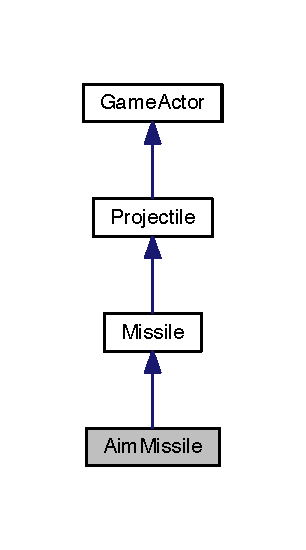
\includegraphics[width=147pt]{class_aim_missile__inherit__graph}
\end{center}
\end{figure}


Collaboration diagram for Aim\+Missile\+:\nopagebreak
\begin{figure}[H]
\begin{center}
\leavevmode
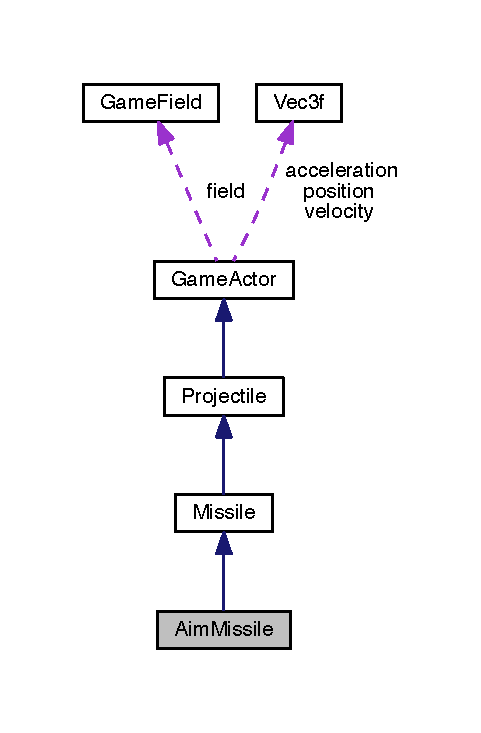
\includegraphics[width=231pt]{class_aim_missile__coll__graph}
\end{center}
\end{figure}
\subsection*{Public Member Functions}
\begin{DoxyCompactItemize}
\item 
\hyperlink{class_aim_missile_ae3683254e6ee78ac44da195df3ab0346}{Aim\+Missile} ()
\item 
\hyperlink{class_aim_missile_af069670ad6122b80380b346d16bb4dfe}{Aim\+Missile} (\hyperlink{class_vec3f}{Vec3f} \hyperlink{class_game_actor_aefed3c91bf32ad388d86657b3bb9ddfa}{position}, \hyperlink{class_vec3f}{Vec3f} \hyperlink{class_game_actor_a95518bf01411eafe983df8815e8682d1}{velocity}, \hyperlink{class_game_field}{Game\+Field} \&\hyperlink{class_game_actor_a0224fbc502abd6b7579787aa234332d5}{field}, \hyperlink{class_game_actor}{Game\+Actor} \&\hyperlink{class_projectile_a54dec73f149e6619fac8f5cf8910edcc}{friendly}, vector$<$ \hyperlink{class_game_actor}{Game\+Actor} $\ast$ $>$ $\ast$\hyperlink{class_game_actor_a2405618d895f5143b42ae9e94d20e693}{actors})
\item 
\hyperlink{class_aim_missile_a6bc3a28a6d9ffb836c546c500767c11b}{Aim\+Missile} (\hyperlink{class_game_actor}{Game\+Actor} \&actor, \hyperlink{class_vec3f}{Vec3f} \hyperlink{class_game_actor_a95518bf01411eafe983df8815e8682d1}{velocity}, \hyperlink{class_game_field}{Game\+Field} \&\hyperlink{class_game_actor_a0224fbc502abd6b7579787aa234332d5}{field}, \hyperlink{class_game_actor}{Game\+Actor} \&\hyperlink{class_projectile_a54dec73f149e6619fac8f5cf8910edcc}{friendly}, vector$<$ \hyperlink{class_game_actor}{Game\+Actor} $\ast$ $>$ $\ast$\hyperlink{class_game_actor_a2405618d895f5143b42ae9e94d20e693}{actors})
\item 
\hyperlink{class_aim_missile_a07cedd9349560318323865759eb7c052}{Aim\+Missile} (\hyperlink{class_game_actor}{Game\+Actor} \&actor, \hyperlink{class_game_field}{Game\+Field} \&\hyperlink{class_game_actor_a0224fbc502abd6b7579787aa234332d5}{field}, \hyperlink{class_game_actor}{Game\+Actor} \&\hyperlink{class_projectile_a54dec73f149e6619fac8f5cf8910edcc}{friendly}, vector$<$ \hyperlink{class_game_actor}{Game\+Actor} $\ast$ $>$ $\ast$\hyperlink{class_game_actor_a2405618d895f5143b42ae9e94d20e693}{actors})
\item 
\hyperlink{class_aim_missile_a26202e854690528be958c6415c652b3d}{Aim\+Missile} (const \hyperlink{class_missile}{Missile} \&projectile)
\item 
\hyperlink{class_aim_missile_af79533845bd96620371edc6b97c4963f}{$\sim$\+Aim\+Missile} ()
\item 
void \hyperlink{class_aim_missile_a2723e6b87d30aa722b795e955a04ddfd}{update} ()
\item 
void \hyperlink{class_aim_missile_aedbbc65c9b383913d3a401bfba40cd4e}{handle\+Collision} (\hyperlink{class_game_actor}{Game\+Actor} \&other)
\end{DoxyCompactItemize}
\subsection*{Additional Inherited Members}


\subsection{Constructor \& Destructor Documentation}
\hypertarget{class_aim_missile_ae3683254e6ee78ac44da195df3ab0346}{\index{Aim\+Missile@{Aim\+Missile}!Aim\+Missile@{Aim\+Missile}}
\index{Aim\+Missile@{Aim\+Missile}!Aim\+Missile@{Aim\+Missile}}
\subsubsection[{Aim\+Missile}]{\setlength{\rightskip}{0pt plus 5cm}Aim\+Missile\+::\+Aim\+Missile (
\begin{DoxyParamCaption}
{}
\end{DoxyParamCaption}
)}}\label{class_aim_missile_ae3683254e6ee78ac44da195df3ab0346}
\hypertarget{class_aim_missile_af069670ad6122b80380b346d16bb4dfe}{\index{Aim\+Missile@{Aim\+Missile}!Aim\+Missile@{Aim\+Missile}}
\index{Aim\+Missile@{Aim\+Missile}!Aim\+Missile@{Aim\+Missile}}
\subsubsection[{Aim\+Missile}]{\setlength{\rightskip}{0pt plus 5cm}Aim\+Missile\+::\+Aim\+Missile (
\begin{DoxyParamCaption}
\item[{{\bf Vec3f}}]{position, }
\item[{{\bf Vec3f}}]{velocity, }
\item[{{\bf Game\+Field} \&}]{field, }
\item[{{\bf Game\+Actor} \&}]{friendly, }
\item[{vector$<$ {\bf Game\+Actor} $\ast$ $>$ $\ast$}]{actors}
\end{DoxyParamCaption}
)}}\label{class_aim_missile_af069670ad6122b80380b346d16bb4dfe}
\hypertarget{class_aim_missile_a6bc3a28a6d9ffb836c546c500767c11b}{\index{Aim\+Missile@{Aim\+Missile}!Aim\+Missile@{Aim\+Missile}}
\index{Aim\+Missile@{Aim\+Missile}!Aim\+Missile@{Aim\+Missile}}
\subsubsection[{Aim\+Missile}]{\setlength{\rightskip}{0pt plus 5cm}Aim\+Missile\+::\+Aim\+Missile (
\begin{DoxyParamCaption}
\item[{{\bf Game\+Actor} \&}]{actor, }
\item[{{\bf Vec3f}}]{velocity, }
\item[{{\bf Game\+Field} \&}]{field, }
\item[{{\bf Game\+Actor} \&}]{friendly, }
\item[{vector$<$ {\bf Game\+Actor} $\ast$ $>$ $\ast$}]{actors}
\end{DoxyParamCaption}
)}}\label{class_aim_missile_a6bc3a28a6d9ffb836c546c500767c11b}
\hypertarget{class_aim_missile_a07cedd9349560318323865759eb7c052}{\index{Aim\+Missile@{Aim\+Missile}!Aim\+Missile@{Aim\+Missile}}
\index{Aim\+Missile@{Aim\+Missile}!Aim\+Missile@{Aim\+Missile}}
\subsubsection[{Aim\+Missile}]{\setlength{\rightskip}{0pt plus 5cm}Aim\+Missile\+::\+Aim\+Missile (
\begin{DoxyParamCaption}
\item[{{\bf Game\+Actor} \&}]{actor, }
\item[{{\bf Game\+Field} \&}]{field, }
\item[{{\bf Game\+Actor} \&}]{friendly, }
\item[{vector$<$ {\bf Game\+Actor} $\ast$ $>$ $\ast$}]{actors}
\end{DoxyParamCaption}
)}}\label{class_aim_missile_a07cedd9349560318323865759eb7c052}
\hypertarget{class_aim_missile_a26202e854690528be958c6415c652b3d}{\index{Aim\+Missile@{Aim\+Missile}!Aim\+Missile@{Aim\+Missile}}
\index{Aim\+Missile@{Aim\+Missile}!Aim\+Missile@{Aim\+Missile}}
\subsubsection[{Aim\+Missile}]{\setlength{\rightskip}{0pt plus 5cm}Aim\+Missile\+::\+Aim\+Missile (
\begin{DoxyParamCaption}
\item[{const {\bf Missile} \&}]{projectile}
\end{DoxyParamCaption}
)}}\label{class_aim_missile_a26202e854690528be958c6415c652b3d}
\hypertarget{class_aim_missile_af79533845bd96620371edc6b97c4963f}{\index{Aim\+Missile@{Aim\+Missile}!````~Aim\+Missile@{$\sim$\+Aim\+Missile}}
\index{````~Aim\+Missile@{$\sim$\+Aim\+Missile}!Aim\+Missile@{Aim\+Missile}}
\subsubsection[{$\sim$\+Aim\+Missile}]{\setlength{\rightskip}{0pt plus 5cm}Aim\+Missile\+::$\sim$\+Aim\+Missile (
\begin{DoxyParamCaption}
{}
\end{DoxyParamCaption}
)}}\label{class_aim_missile_af79533845bd96620371edc6b97c4963f}


\subsection{Member Function Documentation}
\hypertarget{class_aim_missile_aedbbc65c9b383913d3a401bfba40cd4e}{\index{Aim\+Missile@{Aim\+Missile}!handle\+Collision@{handle\+Collision}}
\index{handle\+Collision@{handle\+Collision}!Aim\+Missile@{Aim\+Missile}}
\subsubsection[{handle\+Collision}]{\setlength{\rightskip}{0pt plus 5cm}void Aim\+Missile\+::handle\+Collision (
\begin{DoxyParamCaption}
\item[{{\bf Game\+Actor} \&}]{other}
\end{DoxyParamCaption}
)\hspace{0.3cm}{\ttfamily [virtual]}}}\label{class_aim_missile_aedbbc65c9b383913d3a401bfba40cd4e}
Determines what will happen if this \hyperlink{class_game_actor}{Game\+Actor} collides with another instance of \hyperlink{class_game_actor}{Game\+Actor}. 
\begin{DoxyParams}{Parameters}
{\em other} & the \hyperlink{class_game_actor}{Game\+Actor} colliding with this one \\
\hline
\end{DoxyParams}


Reimplemented from \hyperlink{class_game_actor_aba8cfb1004bf6fc17681cd595b706ada}{Game\+Actor}.



Here is the call graph for this function\+:\nopagebreak
\begin{figure}[H]
\begin{center}
\leavevmode
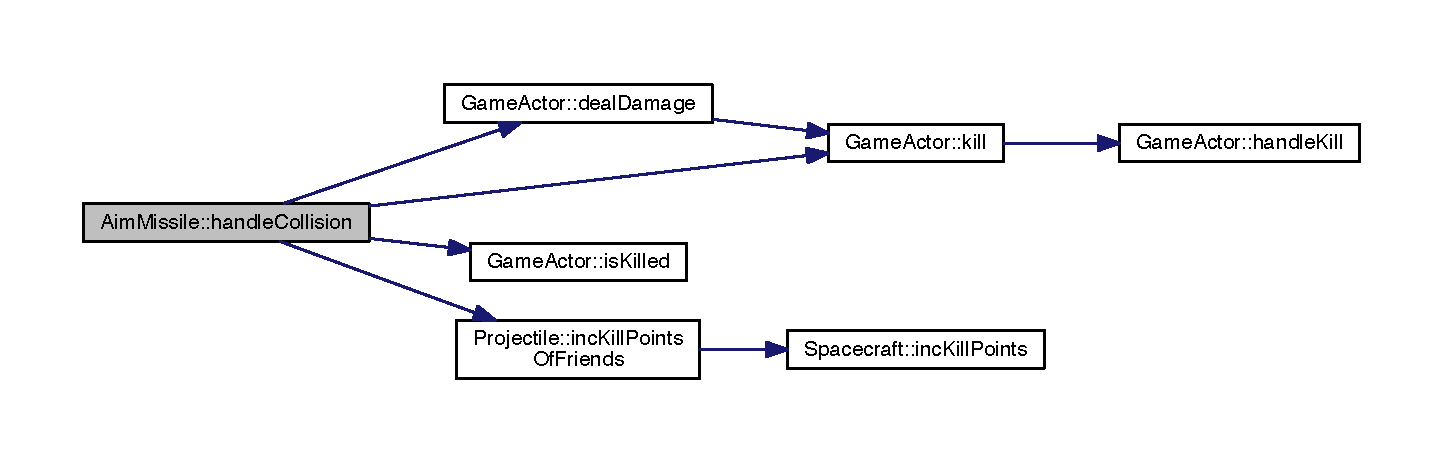
\includegraphics[width=350pt]{class_aim_missile_aedbbc65c9b383913d3a401bfba40cd4e_cgraph}
\end{center}
\end{figure}


\hypertarget{class_aim_missile_a2723e6b87d30aa722b795e955a04ddfd}{\index{Aim\+Missile@{Aim\+Missile}!update@{update}}
\index{update@{update}!Aim\+Missile@{Aim\+Missile}}
\subsubsection[{update}]{\setlength{\rightskip}{0pt plus 5cm}void Aim\+Missile\+::update (
\begin{DoxyParamCaption}
{}
\end{DoxyParamCaption}
)\hspace{0.3cm}{\ttfamily [virtual]}}}\label{class_aim_missile_a2723e6b87d30aa722b795e955a04ddfd}
Updates the position and velocity of this \hyperlink{class_game_actor}{Game\+Actor}. With this implementation Game\+Actors will be bounced off the game field borders. 

Reimplemented from \hyperlink{class_game_actor_ab70229c740251fb7c4222bf579c59393}{Game\+Actor}.



Here is the call graph for this function\+:\nopagebreak
\begin{figure}[H]
\begin{center}
\leavevmode
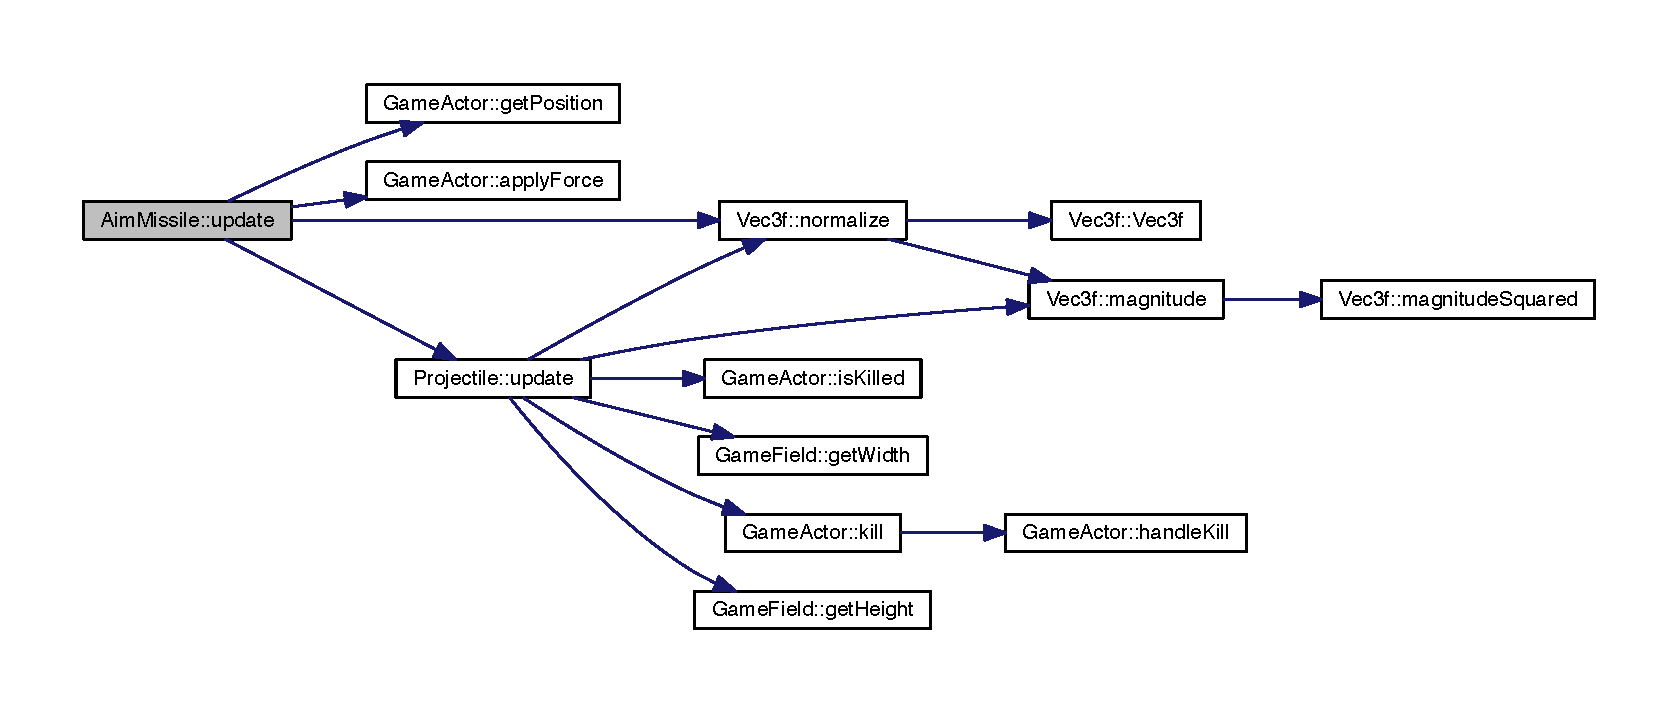
\includegraphics[width=350pt]{class_aim_missile_a2723e6b87d30aa722b795e955a04ddfd_cgraph}
\end{center}
\end{figure}




The documentation for this class was generated from the following files\+:\begin{DoxyCompactItemize}
\item 
src/headers/\hyperlink{_aim_missile_8h}{Aim\+Missile.\+h}\item 
src/\hyperlink{_aim_missile_8cpp}{Aim\+Missile.\+cpp}\end{DoxyCompactItemize}

\hypertarget{class_a_i_player}{\section{A\+I\+Player Class Reference}
\label{class_a_i_player}\index{A\+I\+Player@{A\+I\+Player}}
}


{\ttfamily \#include $<$A\+I\+Player.\+h$>$}



Inheritance diagram for A\+I\+Player\+:\nopagebreak
\begin{figure}[H]
\begin{center}
\leavevmode
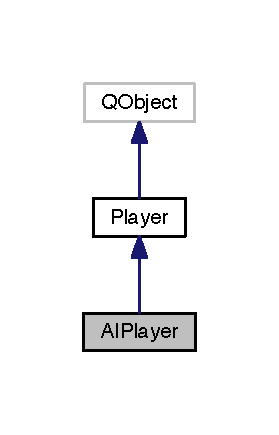
\includegraphics[width=134pt]{class_a_i_player__inherit__graph}
\end{center}
\end{figure}


Collaboration diagram for A\+I\+Player\+:\nopagebreak
\begin{figure}[H]
\begin{center}
\leavevmode
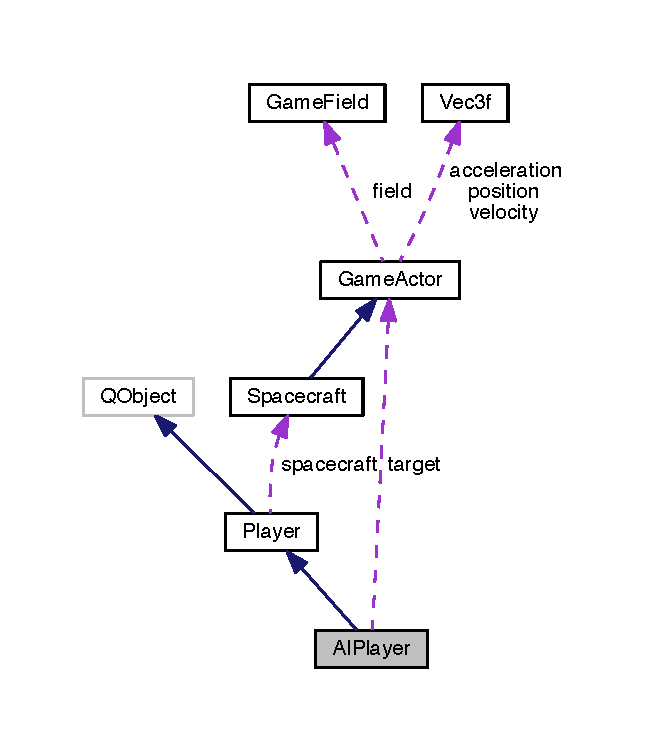
\includegraphics[width=310pt]{class_a_i_player__coll__graph}
\end{center}
\end{figure}
\subsection*{Public Member Functions}
\begin{DoxyCompactItemize}
\item 
\hyperlink{class_a_i_player_a80fe585fd3aa65aeeef5feb52fa76827}{A\+I\+Player} (\hyperlink{class_spacecraft}{Spacecraft} $\ast$\hyperlink{class_player_a7cc88a054d2329b1ca7472a86b2030ca}{spacecraft}, int \hyperlink{class_player_a9528a6db252f2fe947fd7d9189837aec}{frag}, int \hyperlink{class_a_i_player_ae4bc7d7fef8e20ac68867af09b365e21}{difficulty}, std\+::vector$<$ \hyperlink{class_game_actor}{Game\+Actor} $\ast$ $>$ $\ast$\hyperlink{class_a_i_player_a624129174d82f2462320badcd3bfa598}{actors}, Q\+String \hyperlink{class_player_ac41b72814d9c41222dac999bc874280b}{name})
\item 
virtual \hyperlink{class_a_i_player_a2d879575d692d246da3890b6234104b8}{$\sim$\+A\+I\+Player} ()
\item 
void \hyperlink{class_a_i_player_a37a689ed5d72b91e9e1ea2465c9d9b33}{update} ()
\item 
void \hyperlink{class_a_i_player_a21fcfe0e49e5d03ce3954c525aeb33c0}{set\+Actors} (vector$<$ \hyperlink{class_game_actor}{Game\+Actor} $\ast$ $>$ $\ast$\hyperlink{class_a_i_player_a624129174d82f2462320badcd3bfa598}{actors})
\end{DoxyCompactItemize}
\subsection*{Protected Attributes}
\begin{DoxyCompactItemize}
\item 
int \hyperlink{class_a_i_player_ae4bc7d7fef8e20ac68867af09b365e21}{difficulty}
\item 
\hyperlink{class_game_actor}{Game\+Actor} $\ast$ \hyperlink{class_a_i_player_a9380be8a90d97dc0419cb91dfd0e8918}{target}
\item 
vector$<$ \hyperlink{class_game_actor}{Game\+Actor} $\ast$ $>$ $\ast$ \hyperlink{class_a_i_player_a624129174d82f2462320badcd3bfa598}{actors}
\end{DoxyCompactItemize}


\subsection{Constructor \& Destructor Documentation}
\hypertarget{class_a_i_player_a80fe585fd3aa65aeeef5feb52fa76827}{\index{A\+I\+Player@{A\+I\+Player}!A\+I\+Player@{A\+I\+Player}}
\index{A\+I\+Player@{A\+I\+Player}!A\+I\+Player@{A\+I\+Player}}
\subsubsection[{A\+I\+Player}]{\setlength{\rightskip}{0pt plus 5cm}A\+I\+Player\+::\+A\+I\+Player (
\begin{DoxyParamCaption}
\item[{{\bf Spacecraft} $\ast$}]{spacecraft, }
\item[{int}]{frag, }
\item[{int}]{difficulty, }
\item[{std\+::vector$<$ {\bf Game\+Actor} $\ast$ $>$ $\ast$}]{actors, }
\item[{Q\+String}]{name}
\end{DoxyParamCaption}
)}}\label{class_a_i_player_a80fe585fd3aa65aeeef5feb52fa76827}
\hypertarget{class_a_i_player_a2d879575d692d246da3890b6234104b8}{\index{A\+I\+Player@{A\+I\+Player}!````~A\+I\+Player@{$\sim$\+A\+I\+Player}}
\index{````~A\+I\+Player@{$\sim$\+A\+I\+Player}!A\+I\+Player@{A\+I\+Player}}
\subsubsection[{$\sim$\+A\+I\+Player}]{\setlength{\rightskip}{0pt plus 5cm}A\+I\+Player\+::$\sim$\+A\+I\+Player (
\begin{DoxyParamCaption}
{}
\end{DoxyParamCaption}
)\hspace{0.3cm}{\ttfamily [virtual]}}}\label{class_a_i_player_a2d879575d692d246da3890b6234104b8}


\subsection{Member Function Documentation}
\hypertarget{class_a_i_player_a21fcfe0e49e5d03ce3954c525aeb33c0}{\index{A\+I\+Player@{A\+I\+Player}!set\+Actors@{set\+Actors}}
\index{set\+Actors@{set\+Actors}!A\+I\+Player@{A\+I\+Player}}
\subsubsection[{set\+Actors}]{\setlength{\rightskip}{0pt plus 5cm}void A\+I\+Player\+::set\+Actors (
\begin{DoxyParamCaption}
\item[{vector$<$ {\bf Game\+Actor} $\ast$ $>$ $\ast$}]{actors}
\end{DoxyParamCaption}
)}}\label{class_a_i_player_a21fcfe0e49e5d03ce3954c525aeb33c0}
\hypertarget{class_a_i_player_a37a689ed5d72b91e9e1ea2465c9d9b33}{\index{A\+I\+Player@{A\+I\+Player}!update@{update}}
\index{update@{update}!A\+I\+Player@{A\+I\+Player}}
\subsubsection[{update}]{\setlength{\rightskip}{0pt plus 5cm}void A\+I\+Player\+::update (
\begin{DoxyParamCaption}
{}
\end{DoxyParamCaption}
)}}\label{class_a_i_player_a37a689ed5d72b91e9e1ea2465c9d9b33}


Here is the call graph for this function\+:\nopagebreak
\begin{figure}[H]
\begin{center}
\leavevmode
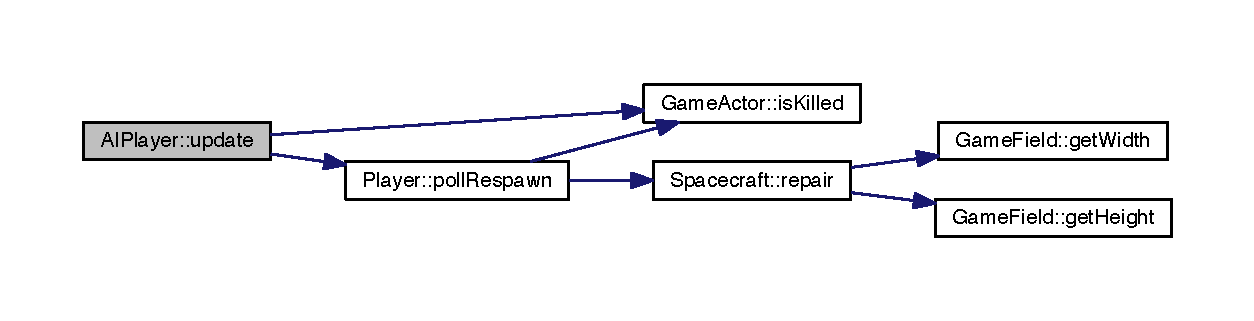
\includegraphics[width=350pt]{class_a_i_player_a37a689ed5d72b91e9e1ea2465c9d9b33_cgraph}
\end{center}
\end{figure}




\subsection{Member Data Documentation}
\hypertarget{class_a_i_player_a624129174d82f2462320badcd3bfa598}{\index{A\+I\+Player@{A\+I\+Player}!actors@{actors}}
\index{actors@{actors}!A\+I\+Player@{A\+I\+Player}}
\subsubsection[{actors}]{\setlength{\rightskip}{0pt plus 5cm}vector$<${\bf Game\+Actor}$\ast$$>$$\ast$ A\+I\+Player\+::actors\hspace{0.3cm}{\ttfamily [protected]}}}\label{class_a_i_player_a624129174d82f2462320badcd3bfa598}
\hypertarget{class_a_i_player_ae4bc7d7fef8e20ac68867af09b365e21}{\index{A\+I\+Player@{A\+I\+Player}!difficulty@{difficulty}}
\index{difficulty@{difficulty}!A\+I\+Player@{A\+I\+Player}}
\subsubsection[{difficulty}]{\setlength{\rightskip}{0pt plus 5cm}int A\+I\+Player\+::difficulty\hspace{0.3cm}{\ttfamily [protected]}}}\label{class_a_i_player_ae4bc7d7fef8e20ac68867af09b365e21}
\hypertarget{class_a_i_player_a9380be8a90d97dc0419cb91dfd0e8918}{\index{A\+I\+Player@{A\+I\+Player}!target@{target}}
\index{target@{target}!A\+I\+Player@{A\+I\+Player}}
\subsubsection[{target}]{\setlength{\rightskip}{0pt plus 5cm}{\bf Game\+Actor}$\ast$ A\+I\+Player\+::target\hspace{0.3cm}{\ttfamily [protected]}}}\label{class_a_i_player_a9380be8a90d97dc0419cb91dfd0e8918}


The documentation for this class was generated from the following files\+:\begin{DoxyCompactItemize}
\item 
src/headers/\hyperlink{_a_i_player_8h}{A\+I\+Player.\+h}\item 
src/\hyperlink{_a_i_player_8cpp}{A\+I\+Player.\+cpp}\end{DoxyCompactItemize}

\hypertarget{class_asteroid}{\section{Asteroid Class Reference}
\label{class_asteroid}\index{Asteroid@{Asteroid}}
}


{\ttfamily \#include $<$Asteroid.\+h$>$}



Inheritance diagram for Asteroid\+:\nopagebreak
\begin{figure}[H]
\begin{center}
\leavevmode
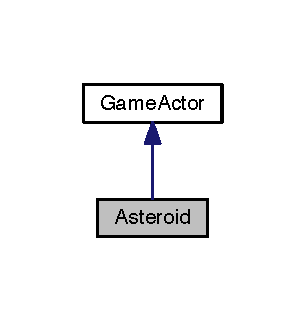
\includegraphics[width=147pt]{class_asteroid__inherit__graph}
\end{center}
\end{figure}


Collaboration diagram for Asteroid\+:\nopagebreak
\begin{figure}[H]
\begin{center}
\leavevmode
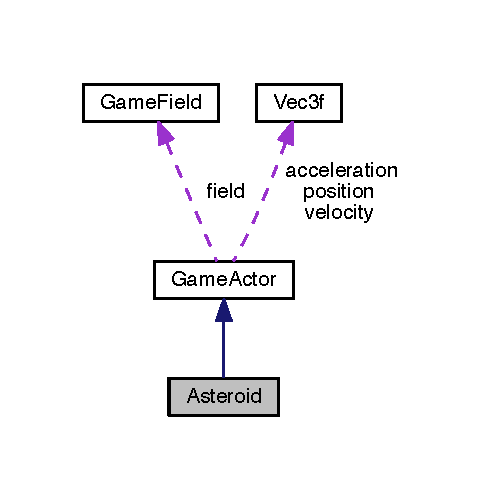
\includegraphics[width=231pt]{class_asteroid__coll__graph}
\end{center}
\end{figure}
\subsection*{Public Member Functions}
\begin{DoxyCompactItemize}
\item 
\hyperlink{class_asteroid_a603c2eb87a4ed26c5b3fb06e953d611c}{Asteroid} ()
\item 
\hyperlink{class_asteroid_a867c9432a4cff5133290762ef6948042}{Asteroid} (\hyperlink{class_vec3f}{Vec3f} \hyperlink{class_game_actor_aefed3c91bf32ad388d86657b3bb9ddfa}{position}, double \hyperlink{class_game_actor_a2111233f4f0216db4d172d5088ebeed4}{mass}, float \hyperlink{class_game_actor_a9c0ba51b08a3e617d9629c0ee8d309f2}{gravitation\+Range}, float \hyperlink{class_game_actor_a42ed4bef0d99cf053ff9a025c86d34d3}{g}, \hyperlink{class_game_field}{Game\+Field} \&\hyperlink{class_game_actor_a0224fbc502abd6b7579787aa234332d5}{field}, float \hyperlink{class_game_actor_a15b6abd006c52b21c569932f8b484eb0}{max\+Speed}, vector$<$ \hyperlink{class_game_actor}{Game\+Actor} $\ast$ $>$ $\ast$\hyperlink{class_game_actor_a2405618d895f5143b42ae9e94d20e693}{actors})
\item 
void \hyperlink{class_asteroid_ada68cafcbb9e41c90f3e372de1a4b0ba}{handle\+Collision} (\hyperlink{class_game_actor}{Game\+Actor} \&other)
\item 
\hyperlink{class_game_actor_view}{Game\+Actor\+View} $\ast$ \hyperlink{class_asteroid_a267c313e8759ca6091455616cc6c40f1}{get\+View} () const 
\end{DoxyCompactItemize}
\subsection*{Additional Inherited Members}


\subsection{Constructor \& Destructor Documentation}
\hypertarget{class_asteroid_a603c2eb87a4ed26c5b3fb06e953d611c}{\index{Asteroid@{Asteroid}!Asteroid@{Asteroid}}
\index{Asteroid@{Asteroid}!Asteroid@{Asteroid}}
\subsubsection[{Asteroid}]{\setlength{\rightskip}{0pt plus 5cm}Asteroid\+::\+Asteroid (
\begin{DoxyParamCaption}
{}
\end{DoxyParamCaption}
)}}\label{class_asteroid_a603c2eb87a4ed26c5b3fb06e953d611c}
\hypertarget{class_asteroid_a867c9432a4cff5133290762ef6948042}{\index{Asteroid@{Asteroid}!Asteroid@{Asteroid}}
\index{Asteroid@{Asteroid}!Asteroid@{Asteroid}}
\subsubsection[{Asteroid}]{\setlength{\rightskip}{0pt plus 5cm}Asteroid\+::\+Asteroid (
\begin{DoxyParamCaption}
\item[{{\bf Vec3f}}]{position, }
\item[{double}]{mass, }
\item[{float}]{gravitation\+Range, }
\item[{float}]{g, }
\item[{{\bf Game\+Field} \&}]{field, }
\item[{float}]{max\+Speed, }
\item[{vector$<$ {\bf Game\+Actor} $\ast$ $>$ $\ast$}]{actors}
\end{DoxyParamCaption}
)}}\label{class_asteroid_a867c9432a4cff5133290762ef6948042}


\subsection{Member Function Documentation}
\hypertarget{class_asteroid_a267c313e8759ca6091455616cc6c40f1}{\index{Asteroid@{Asteroid}!get\+View@{get\+View}}
\index{get\+View@{get\+View}!Asteroid@{Asteroid}}
\subsubsection[{get\+View}]{\setlength{\rightskip}{0pt plus 5cm}{\bf Game\+Actor\+View} $\ast$ Asteroid\+::get\+View (
\begin{DoxyParamCaption}
{}
\end{DoxyParamCaption}
) const\hspace{0.3cm}{\ttfamily [virtual]}}}\label{class_asteroid_a267c313e8759ca6091455616cc6c40f1}
Creates and returns a \hyperlink{class_game_actor_view}{Game\+Actor\+View} of this instance of \hyperlink{class_game_actor}{Game\+Actor}. \begin{DoxyReturn}{Returns}
the \hyperlink{class_game_actor_view}{Game\+Actor\+View} for this \hyperlink{class_game_actor}{Game\+Actor} 
\end{DoxyReturn}


Reimplemented from \hyperlink{class_game_actor_ae63b522db0d88f56e3c7a8cfb60d31a6}{Game\+Actor}.



Here is the call graph for this function\+:\nopagebreak
\begin{figure}[H]
\begin{center}
\leavevmode
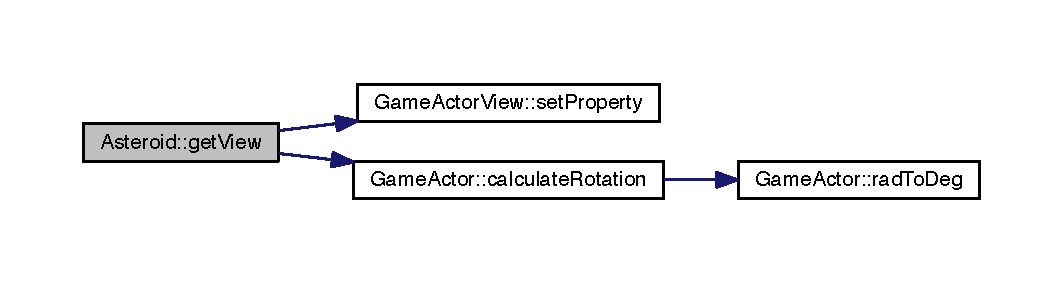
\includegraphics[width=350pt]{class_asteroid_a267c313e8759ca6091455616cc6c40f1_cgraph}
\end{center}
\end{figure}


\hypertarget{class_asteroid_ada68cafcbb9e41c90f3e372de1a4b0ba}{\index{Asteroid@{Asteroid}!handle\+Collision@{handle\+Collision}}
\index{handle\+Collision@{handle\+Collision}!Asteroid@{Asteroid}}
\subsubsection[{handle\+Collision}]{\setlength{\rightskip}{0pt plus 5cm}void Asteroid\+::handle\+Collision (
\begin{DoxyParamCaption}
\item[{{\bf Game\+Actor} \&}]{other}
\end{DoxyParamCaption}
)\hspace{0.3cm}{\ttfamily [virtual]}}}\label{class_asteroid_ada68cafcbb9e41c90f3e372de1a4b0ba}
Determines what will happen if this \hyperlink{class_game_actor}{Game\+Actor} collides with another instance of \hyperlink{class_game_actor}{Game\+Actor}. 
\begin{DoxyParams}{Parameters}
{\em other} & the \hyperlink{class_game_actor}{Game\+Actor} colliding with this one \\
\hline
\end{DoxyParams}


Reimplemented from \hyperlink{class_game_actor_aba8cfb1004bf6fc17681cd595b706ada}{Game\+Actor}.



Here is the call graph for this function\+:\nopagebreak
\begin{figure}[H]
\begin{center}
\leavevmode
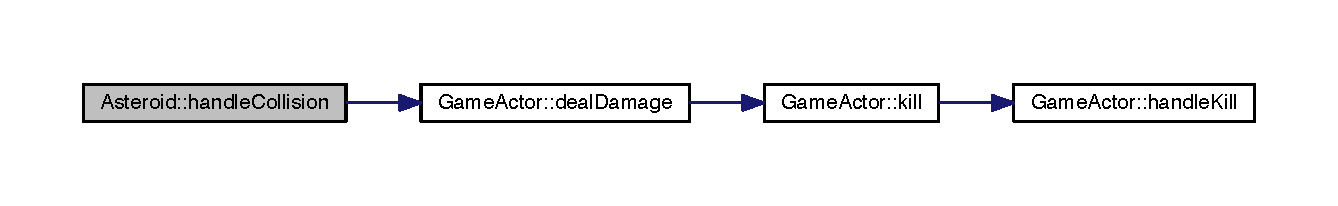
\includegraphics[width=350pt]{class_asteroid_ada68cafcbb9e41c90f3e372de1a4b0ba_cgraph}
\end{center}
\end{figure}




The documentation for this class was generated from the following files\+:\begin{DoxyCompactItemize}
\item 
src/headers/\hyperlink{_asteroid_8h}{Asteroid.\+h}\item 
src/\hyperlink{_asteroid_8cpp}{Asteroid.\+cpp}\end{DoxyCompactItemize}

\hypertarget{class_game}{\section{Game Class Reference}
\label{class_game}\index{Game@{Game}}
}


{\ttfamily \#include $<$Game.\+h$>$}



Inheritance diagram for Game\+:\nopagebreak
\begin{figure}[H]
\begin{center}
\leavevmode
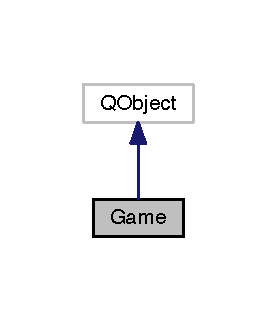
\includegraphics[width=133pt]{class_game__inherit__graph}
\end{center}
\end{figure}


Collaboration diagram for Game\+:\nopagebreak
\begin{figure}[H]
\begin{center}
\leavevmode
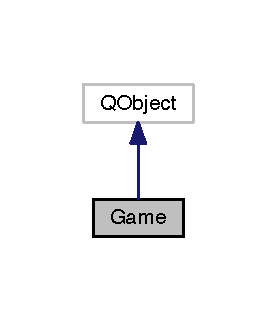
\includegraphics[width=133pt]{class_game__coll__graph}
\end{center}
\end{figure}
\subsection*{Public Slots}
\begin{DoxyCompactItemize}
\item 
void \hyperlink{class_game_a645389b61e4d2fb43691208651c5a4e2}{render} (vector$<$ \hyperlink{class_game_actor_view}{Game\+Actor\+View} $\ast$ $>$ $\ast$views)
\item 
void \hyperlink{class_game_aab513bbe5db45b1f9dba205d0ddec74e}{render\+Remote} (Q\+String views)
\item 
void \hyperlink{class_game_a226a897819cb653c61868cbf96b90ad5}{set\+Active\+Weapon} (int weapon\+Number)
\item 
void \hyperlink{class_game_a60ef32ef5040d639aaae74c74466e186}{set\+Lifepoints} (int lifepoints)
\item 
void \hyperlink{class_game_a9955838a261e9c1aee21bc6746f11f4f}{set\+Background\+Position} (float x, float y, float field\+Width, float field\+Height)
\item 
void \hyperlink{class_game_a59f88c64cc14f60ec2d7d3f94d1e00e7}{set\+Infobox\+Message} (Q\+String message)
\item 
void \hyperlink{class_game_a8cbceafcfbb9fe7d67827c428f8f0ee6}{set\+Frag} (int must, int have)
\end{DoxyCompactItemize}
\subsection*{Public Member Functions}
\begin{DoxyCompactItemize}
\item 
\hyperlink{class_game_a1875963fc898101a29d47084aebffa28}{Game} (Q\+Object $\ast$parent=0)
\item 
\hyperlink{class_game_afeda9924813b108f34ca94e1d5ead7c9}{Game} (Q\+Qml\+Application\+Engine $\ast$the\+Engine, \hyperlink{class_gravitron_settings}{Gravitron\+Settings} $\ast$the\+Settings, \hyperlink{class_tcp_client}{Tcp\+Client} $\ast$client, \hyperlink{class_tcp_server}{Tcp\+Server} $\ast$server)
\item 
\hyperlink{class_game_ae3d112ca6e0e55150d2fdbc704474530}{$\sim$\+Game} ()
\item 
Q\+\_\+\+I\+N\+V\+O\+K\+A\+B\+L\+E void \hyperlink{class_game_ac7edf2d1ecf3e7e450a5c2b5489945f0}{set\+Qml\+Parent} (Q\+Quick\+Item $\ast$the\+Qml\+Parent)
\item 
Q\+\_\+\+I\+N\+V\+O\+K\+A\+B\+L\+E void \hyperlink{class_game_a3d9b98f7c4a96ecf578f75b96c9f0e90}{start} ()
\item 
Q\+\_\+\+I\+N\+V\+O\+K\+A\+B\+L\+E void \hyperlink{class_game_a25c97b9eb158946f4b10993dfc3cf6f3}{start\+Client} ()
\item 
Q\+\_\+\+I\+N\+V\+O\+K\+A\+B\+L\+E void \hyperlink{class_game_aed51d3d3760d9c052cdf33144ead0fba}{start\+Server} ()
\item 
Q\+\_\+\+I\+N\+V\+O\+K\+A\+B\+L\+E void \hyperlink{class_game_a17fbb36fd4a2085f9ff4f1fa93d7d08b}{stop} ()
\end{DoxyCompactItemize}


\subsection{Constructor \& Destructor Documentation}
\hypertarget{class_game_a1875963fc898101a29d47084aebffa28}{\index{Game@{Game}!Game@{Game}}
\index{Game@{Game}!Game@{Game}}
\subsubsection[{Game}]{\setlength{\rightskip}{0pt plus 5cm}Game\+::\+Game (
\begin{DoxyParamCaption}
\item[{Q\+Object $\ast$}]{parent = {\ttfamily 0}}
\end{DoxyParamCaption}
)}}\label{class_game_a1875963fc898101a29d47084aebffa28}
\hypertarget{class_game_afeda9924813b108f34ca94e1d5ead7c9}{\index{Game@{Game}!Game@{Game}}
\index{Game@{Game}!Game@{Game}}
\subsubsection[{Game}]{\setlength{\rightskip}{0pt plus 5cm}Game\+::\+Game (
\begin{DoxyParamCaption}
\item[{Q\+Qml\+Application\+Engine $\ast$}]{the\+Engine, }
\item[{{\bf Gravitron\+Settings} $\ast$}]{the\+Settings, }
\item[{{\bf Tcp\+Client} $\ast$}]{client, }
\item[{{\bf Tcp\+Server} $\ast$}]{server}
\end{DoxyParamCaption}
)}}\label{class_game_afeda9924813b108f34ca94e1d5ead7c9}
\hypertarget{class_game_ae3d112ca6e0e55150d2fdbc704474530}{\index{Game@{Game}!````~Game@{$\sim$\+Game}}
\index{````~Game@{$\sim$\+Game}!Game@{Game}}
\subsubsection[{$\sim$\+Game}]{\setlength{\rightskip}{0pt plus 5cm}Game\+::$\sim$\+Game (
\begin{DoxyParamCaption}
{}
\end{DoxyParamCaption}
)}}\label{class_game_ae3d112ca6e0e55150d2fdbc704474530}


Here is the call graph for this function\+:\nopagebreak
\begin{figure}[H]
\begin{center}
\leavevmode
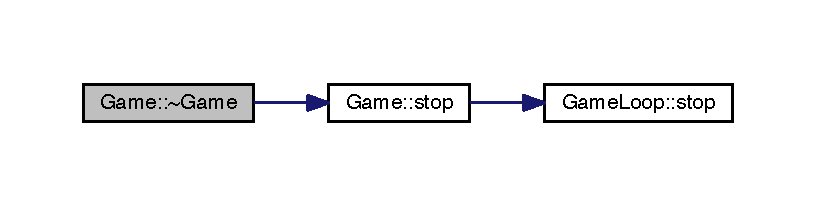
\includegraphics[width=350pt]{class_game_ae3d112ca6e0e55150d2fdbc704474530_cgraph}
\end{center}
\end{figure}




\subsection{Member Function Documentation}
\hypertarget{class_game_a645389b61e4d2fb43691208651c5a4e2}{\index{Game@{Game}!render@{render}}
\index{render@{render}!Game@{Game}}
\subsubsection[{render}]{\setlength{\rightskip}{0pt plus 5cm}void Game\+::render (
\begin{DoxyParamCaption}
\item[{vector$<$ {\bf Game\+Actor\+View} $\ast$ $>$ $\ast$}]{views}
\end{DoxyParamCaption}
)\hspace{0.3cm}{\ttfamily [slot]}}}\label{class_game_a645389b61e4d2fb43691208651c5a4e2}
Creates a Q\+Quick\+Item for each element in the views list and adds their special properties.

I\+M\+P\+O\+R\+T\+A\+N\+T! The list and its content gets deleted from the heap!


\begin{DoxyParams}{Parameters}
{\em views} & pointer to a vector of pointers to \hyperlink{class_game_actor_view}{Game\+Actor\+View}'s \\
\hline
\end{DoxyParams}


Here is the call graph for this function\+:\nopagebreak
\begin{figure}[H]
\begin{center}
\leavevmode
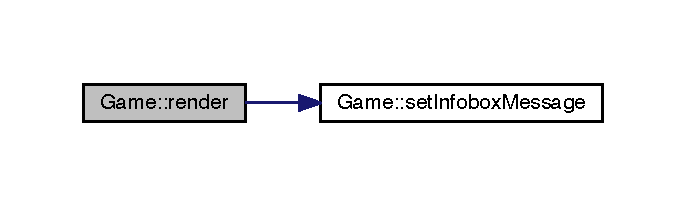
\includegraphics[width=329pt]{class_game_a645389b61e4d2fb43691208651c5a4e2_cgraph}
\end{center}
\end{figure}


\hypertarget{class_game_aab513bbe5db45b1f9dba205d0ddec74e}{\index{Game@{Game}!render\+Remote@{render\+Remote}}
\index{render\+Remote@{render\+Remote}!Game@{Game}}
\subsubsection[{render\+Remote}]{\setlength{\rightskip}{0pt plus 5cm}void Game\+::render\+Remote (
\begin{DoxyParamCaption}
\item[{Q\+String}]{serialized\+Viewlist}
\end{DoxyParamCaption}
)\hspace{0.3cm}{\ttfamily [slot]}}}\label{class_game_aab513bbe5db45b1f9dba205d0ddec74e}
Deserializes the serialized Views, generates a viewlist and sends them to the render method.


\begin{DoxyParams}{Parameters}
{\em serialized\+Viewlist} & Qstring of the serialized\+Viewlist over the network. \\
\hline
\end{DoxyParams}


Here is the call graph for this function\+:\nopagebreak
\begin{figure}[H]
\begin{center}
\leavevmode
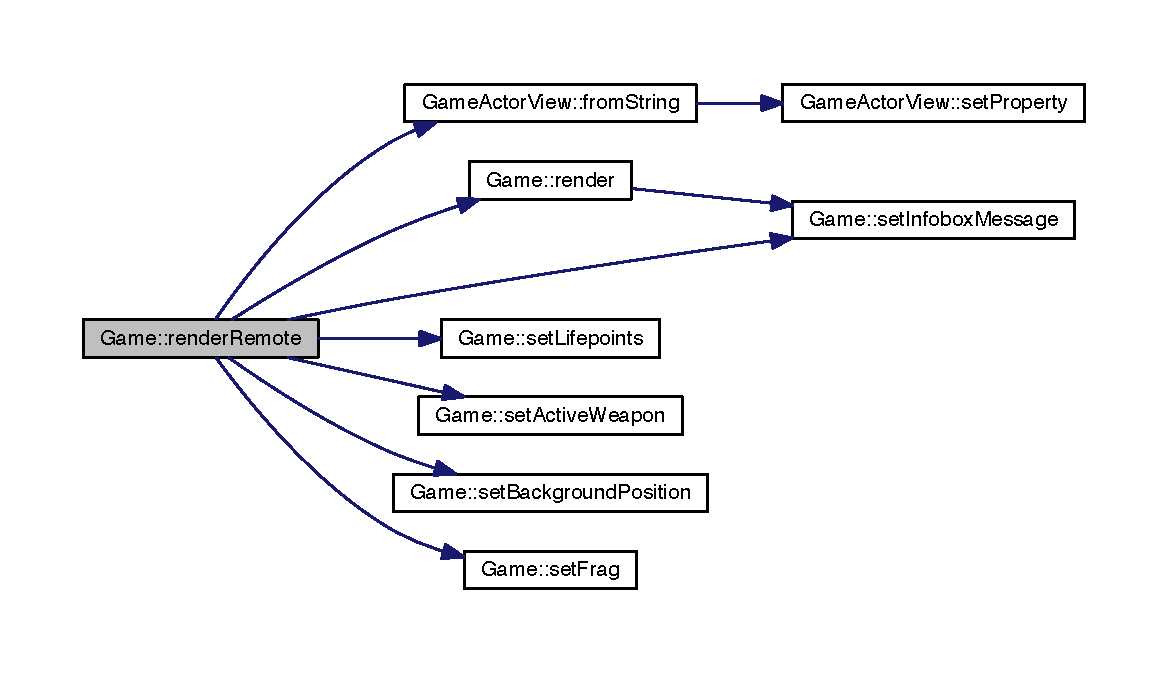
\includegraphics[width=350pt]{class_game_aab513bbe5db45b1f9dba205d0ddec74e_cgraph}
\end{center}
\end{figure}


\hypertarget{class_game_a226a897819cb653c61868cbf96b90ad5}{\index{Game@{Game}!set\+Active\+Weapon@{set\+Active\+Weapon}}
\index{set\+Active\+Weapon@{set\+Active\+Weapon}!Game@{Game}}
\subsubsection[{set\+Active\+Weapon}]{\setlength{\rightskip}{0pt plus 5cm}void Game\+::set\+Active\+Weapon (
\begin{DoxyParamCaption}
\item[{int}]{weapon\+Number}
\end{DoxyParamCaption}
)\hspace{0.3cm}{\ttfamily [slot]}}}\label{class_game_a226a897819cb653c61868cbf96b90ad5}
\hypertarget{class_game_a9955838a261e9c1aee21bc6746f11f4f}{\index{Game@{Game}!set\+Background\+Position@{set\+Background\+Position}}
\index{set\+Background\+Position@{set\+Background\+Position}!Game@{Game}}
\subsubsection[{set\+Background\+Position}]{\setlength{\rightskip}{0pt plus 5cm}void Game\+::set\+Background\+Position (
\begin{DoxyParamCaption}
\item[{float}]{x, }
\item[{float}]{y, }
\item[{float}]{field\+Width, }
\item[{float}]{field\+Height}
\end{DoxyParamCaption}
)\hspace{0.3cm}{\ttfamily [slot]}}}\label{class_game_a9955838a261e9c1aee21bc6746f11f4f}
\hypertarget{class_game_a8cbceafcfbb9fe7d67827c428f8f0ee6}{\index{Game@{Game}!set\+Frag@{set\+Frag}}
\index{set\+Frag@{set\+Frag}!Game@{Game}}
\subsubsection[{set\+Frag}]{\setlength{\rightskip}{0pt plus 5cm}void Game\+::set\+Frag (
\begin{DoxyParamCaption}
\item[{int}]{must, }
\item[{int}]{have}
\end{DoxyParamCaption}
)\hspace{0.3cm}{\ttfamily [slot]}}}\label{class_game_a8cbceafcfbb9fe7d67827c428f8f0ee6}
\hypertarget{class_game_a59f88c64cc14f60ec2d7d3f94d1e00e7}{\index{Game@{Game}!set\+Infobox\+Message@{set\+Infobox\+Message}}
\index{set\+Infobox\+Message@{set\+Infobox\+Message}!Game@{Game}}
\subsubsection[{set\+Infobox\+Message}]{\setlength{\rightskip}{0pt plus 5cm}void Game\+::set\+Infobox\+Message (
\begin{DoxyParamCaption}
\item[{Q\+String}]{message}
\end{DoxyParamCaption}
)\hspace{0.3cm}{\ttfamily [slot]}}}\label{class_game_a59f88c64cc14f60ec2d7d3f94d1e00e7}
\hypertarget{class_game_a60ef32ef5040d639aaae74c74466e186}{\index{Game@{Game}!set\+Lifepoints@{set\+Lifepoints}}
\index{set\+Lifepoints@{set\+Lifepoints}!Game@{Game}}
\subsubsection[{set\+Lifepoints}]{\setlength{\rightskip}{0pt plus 5cm}void Game\+::set\+Lifepoints (
\begin{DoxyParamCaption}
\item[{int}]{lifepoints}
\end{DoxyParamCaption}
)\hspace{0.3cm}{\ttfamily [slot]}}}\label{class_game_a60ef32ef5040d639aaae74c74466e186}
\hypertarget{class_game_ac7edf2d1ecf3e7e450a5c2b5489945f0}{\index{Game@{Game}!set\+Qml\+Parent@{set\+Qml\+Parent}}
\index{set\+Qml\+Parent@{set\+Qml\+Parent}!Game@{Game}}
\subsubsection[{set\+Qml\+Parent}]{\setlength{\rightskip}{0pt plus 5cm}void Game\+::set\+Qml\+Parent (
\begin{DoxyParamCaption}
\item[{Q\+Quick\+Item $\ast$}]{the\+Qml\+Parent}
\end{DoxyParamCaption}
)}}\label{class_game_ac7edf2d1ecf3e7e450a5c2b5489945f0}
Setter for the Q\+Quick\+Item which acts as the same scene.


\begin{DoxyParams}{Parameters}
{\em the\+Qml\+Parent} & \\
\hline
\end{DoxyParams}
\hypertarget{class_game_a3d9b98f7c4a96ecf578f75b96c9f0e90}{\index{Game@{Game}!start@{start}}
\index{start@{start}!Game@{Game}}
\subsubsection[{start}]{\setlength{\rightskip}{0pt plus 5cm}void Game\+::start (
\begin{DoxyParamCaption}
{}
\end{DoxyParamCaption}
)}}\label{class_game_a3d9b98f7c4a96ecf578f75b96c9f0e90}
Initializes the \hyperlink{class_game_loop}{Game\+Loop} in a own thread and connects the singnals/slots. 

Here is the call graph for this function\+:\nopagebreak
\begin{figure}[H]
\begin{center}
\leavevmode
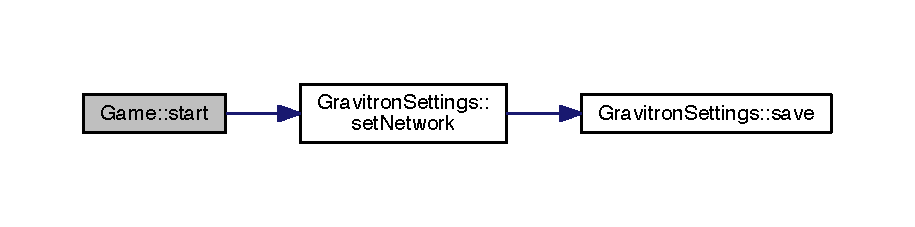
\includegraphics[width=350pt]{class_game_a3d9b98f7c4a96ecf578f75b96c9f0e90_cgraph}
\end{center}
\end{figure}


\hypertarget{class_game_a25c97b9eb158946f4b10993dfc3cf6f3}{\index{Game@{Game}!start\+Client@{start\+Client}}
\index{start\+Client@{start\+Client}!Game@{Game}}
\subsubsection[{start\+Client}]{\setlength{\rightskip}{0pt plus 5cm}void Game\+::start\+Client (
\begin{DoxyParamCaption}
{}
\end{DoxyParamCaption}
)}}\label{class_game_a25c97b9eb158946f4b10993dfc3cf6f3}


Here is the call graph for this function\+:\nopagebreak
\begin{figure}[H]
\begin{center}
\leavevmode
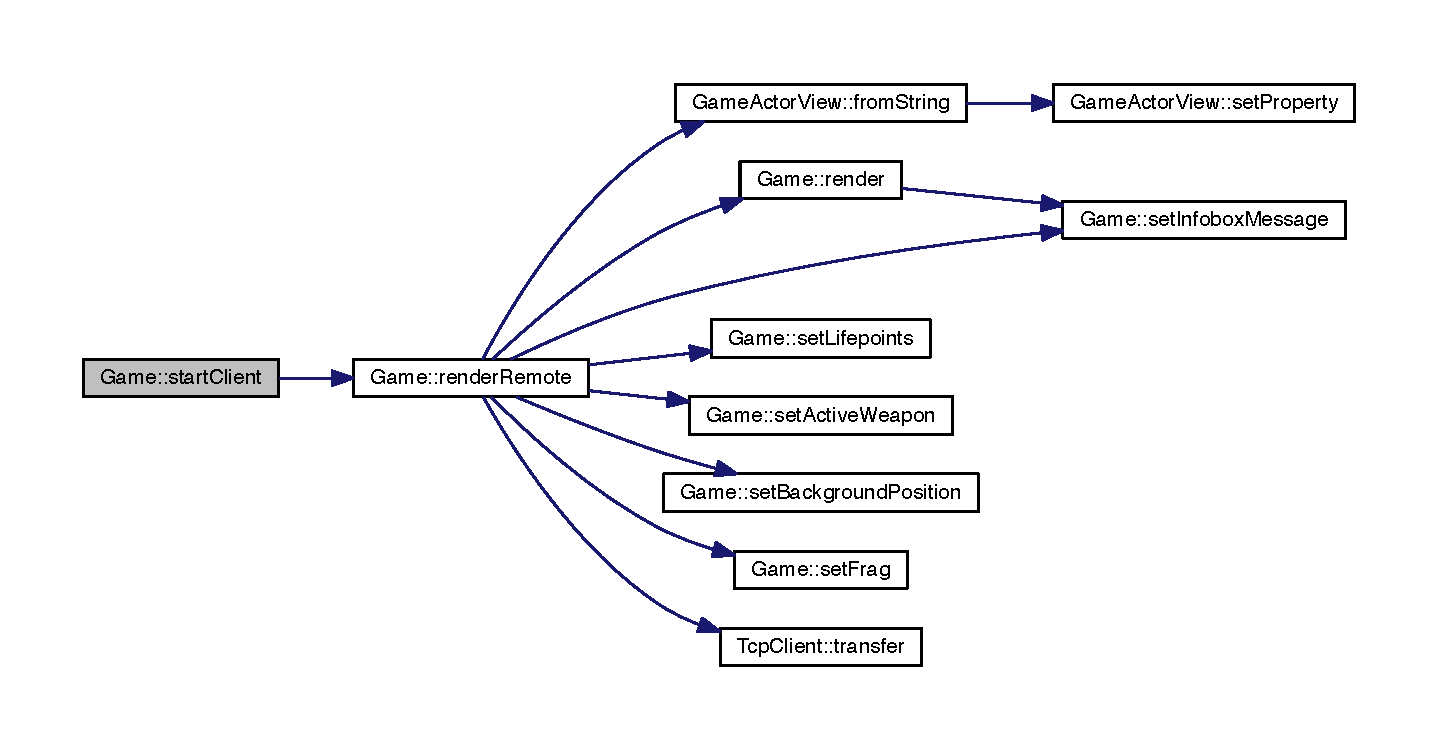
\includegraphics[width=350pt]{class_game_a25c97b9eb158946f4b10993dfc3cf6f3_cgraph}
\end{center}
\end{figure}


\hypertarget{class_game_aed51d3d3760d9c052cdf33144ead0fba}{\index{Game@{Game}!start\+Server@{start\+Server}}
\index{start\+Server@{start\+Server}!Game@{Game}}
\subsubsection[{start\+Server}]{\setlength{\rightskip}{0pt plus 5cm}void Game\+::start\+Server (
\begin{DoxyParamCaption}
{}
\end{DoxyParamCaption}
)}}\label{class_game_aed51d3d3760d9c052cdf33144ead0fba}


Here is the call graph for this function\+:\nopagebreak
\begin{figure}[H]
\begin{center}
\leavevmode
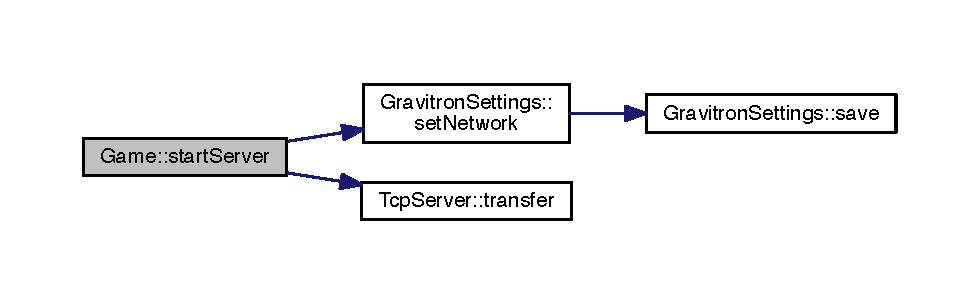
\includegraphics[width=350pt]{class_game_aed51d3d3760d9c052cdf33144ead0fba_cgraph}
\end{center}
\end{figure}


\hypertarget{class_game_a17fbb36fd4a2085f9ff4f1fa93d7d08b}{\index{Game@{Game}!stop@{stop}}
\index{stop@{stop}!Game@{Game}}
\subsubsection[{stop}]{\setlength{\rightskip}{0pt plus 5cm}void Game\+::stop (
\begin{DoxyParamCaption}
{}
\end{DoxyParamCaption}
)}}\label{class_game_a17fbb36fd4a2085f9ff4f1fa93d7d08b}


Here is the call graph for this function\+:\nopagebreak
\begin{figure}[H]
\begin{center}
\leavevmode
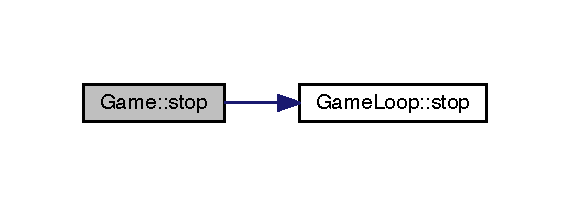
\includegraphics[width=274pt]{class_game_a17fbb36fd4a2085f9ff4f1fa93d7d08b_cgraph}
\end{center}
\end{figure}




The documentation for this class was generated from the following files\+:\begin{DoxyCompactItemize}
\item 
src/headers/\hyperlink{_game_8h}{Game.\+h}\item 
src/\hyperlink{_game_8cpp}{Game.\+cpp}\end{DoxyCompactItemize}

\hypertarget{class_game_actor}{\section{Game\+Actor Class Reference}
\label{class_game_actor}\index{Game\+Actor@{Game\+Actor}}
}


{\ttfamily \#include $<$Game\+Actor.\+h$>$}



Inheritance diagram for Game\+Actor\+:\nopagebreak
\begin{figure}[H]
\begin{center}
\leavevmode
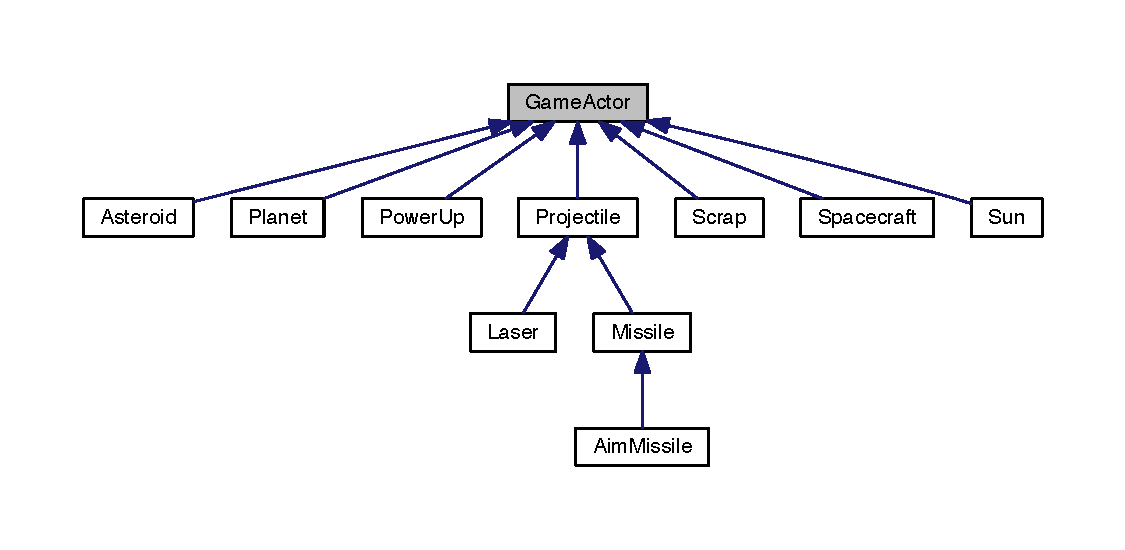
\includegraphics[width=350pt]{class_game_actor__inherit__graph}
\end{center}
\end{figure}


Collaboration diagram for Game\+Actor\+:\nopagebreak
\begin{figure}[H]
\begin{center}
\leavevmode
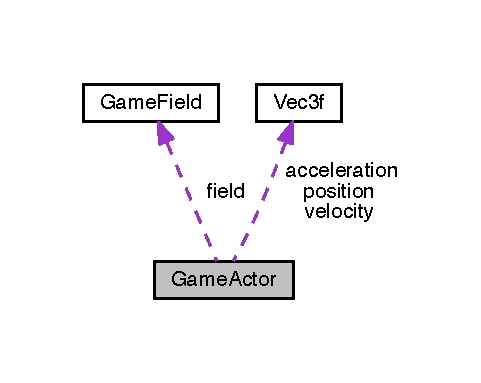
\includegraphics[width=231pt]{class_game_actor__coll__graph}
\end{center}
\end{figure}
\subsection*{Public Member Functions}
\begin{DoxyCompactItemize}
\item 
\hyperlink{class_game_actor_a15b04d8c6628c4d004573c3facfdb418}{Game\+Actor} ()
\item 
\hyperlink{class_game_actor_a8419e87ea13e15b82ed1564e477377ac}{Game\+Actor} (\hyperlink{class_vec3f}{Vec3f} \hyperlink{class_game_actor_aefed3c91bf32ad388d86657b3bb9ddfa}{position}, double \hyperlink{class_game_actor_a2111233f4f0216db4d172d5088ebeed4}{mass}, float \hyperlink{class_game_actor_a9c0ba51b08a3e617d9629c0ee8d309f2}{gravitation\+Range}, float \hyperlink{class_game_actor_a42ed4bef0d99cf053ff9a025c86d34d3}{g}, int \hyperlink{class_game_actor_a5d402a953140585fb7cc3f8a3a24a2a4}{health}, \hyperlink{class_game_field}{Game\+Field} \&\hyperlink{class_game_actor_a0224fbc502abd6b7579787aa234332d5}{field}, vector$<$ \hyperlink{class_game_actor}{Game\+Actor} $\ast$ $>$ $\ast$\hyperlink{class_game_actor_a2405618d895f5143b42ae9e94d20e693}{actors})
\item 
\hyperlink{class_game_actor_aad104099e725fa6224de80dbaf52f2b1}{Game\+Actor} (\hyperlink{class_vec3f}{Vec3f} \hyperlink{class_game_actor_aefed3c91bf32ad388d86657b3bb9ddfa}{position}, double \hyperlink{class_game_actor_a2111233f4f0216db4d172d5088ebeed4}{mass}, float \hyperlink{class_game_actor_a9c0ba51b08a3e617d9629c0ee8d309f2}{gravitation\+Range}, float \hyperlink{class_game_actor_a42ed4bef0d99cf053ff9a025c86d34d3}{g}, int \hyperlink{class_game_actor_a5d402a953140585fb7cc3f8a3a24a2a4}{health}, \hyperlink{class_game_field}{Game\+Field} \&\hyperlink{class_game_actor_a0224fbc502abd6b7579787aa234332d5}{field}, float \hyperlink{class_game_actor_a15b6abd006c52b21c569932f8b484eb0}{max\+Speed}, vector$<$ \hyperlink{class_game_actor}{Game\+Actor} $\ast$ $>$ $\ast$\hyperlink{class_game_actor_a2405618d895f5143b42ae9e94d20e693}{actors})
\item 
\hyperlink{class_game_actor_a305c6d8136305e8bfc72e2b64f44f549}{Game\+Actor} (const \hyperlink{class_game_actor}{Game\+Actor} \&actor)
\item 
bool \hyperlink{class_game_actor_a6052cc4a43b18dc72103a5a1abc521c2}{operator==} (\hyperlink{class_game_actor}{Game\+Actor} \&right)
\item 
\hyperlink{class_game_actor}{Game\+Actor} \& \hyperlink{class_game_actor_a806e4306d891e32c4e06b961cbf11702}{operator=} (const \hyperlink{class_game_actor}{Game\+Actor} \&right)
\item 
\hyperlink{class_vec3f}{Vec3f} \hyperlink{class_game_actor_a8a0ca1b6866225d66df2381649bdc601}{get\+Position} () const 
\item 
\hyperlink{class_vec3f}{Vec3f} \hyperlink{class_game_actor_aa50b1f399dc19a4dd62995641465cbd2}{get\+Acceleration} () const 
\item 
\hyperlink{class_vec3f}{Vec3f} \hyperlink{class_game_actor_a1f624837eac0fe9fe80bcb54cfe8b1cf}{get\+Velocity} () const 
\item 
float \hyperlink{class_game_actor_ac19034996d2c622f4f2fd5870d43c9cd}{get\+Mass} () const 
\item 
float \hyperlink{class_game_actor_adb2e41937471e0f7377a188f399684cf}{get\+Gravitation\+Range} () const 
\item 
float \hyperlink{class_game_actor_a7fafd913a7b0f93d66f7335c8e8417f9}{get\+G} () const 
\item 
void \hyperlink{class_game_actor_af3fbd8b984fdd0df93cc4c6f342caa5e}{set\+G} (float \hyperlink{class_game_actor_a42ed4bef0d99cf053ff9a025c86d34d3}{g})
\item 
float \hyperlink{class_game_actor_a13cec4e211c56989b4ef58ead7c31e17}{get\+Max\+Speed} () const 
\item 
void \hyperlink{class_game_actor_a33f79600c44e3372a23c3ca2ee880704}{set\+Max\+Speed} (float \hyperlink{class_game_actor_a15b6abd006c52b21c569932f8b484eb0}{max\+Speed})
\item 
int \hyperlink{class_game_actor_a0e29a446b3247da54893ef12faa9eaaa}{get\+Health} () const 
\item 
void \hyperlink{class_game_actor_ace7f2c9f95ac3c39acbb88a3c31240b4}{set\+Health} (int \hyperlink{class_game_actor_a5d402a953140585fb7cc3f8a3a24a2a4}{health})
\item 
void \hyperlink{class_game_actor_a168ddb4dda02a8dd734f35d61e325de9}{deal\+Damage} (int damage)
\item 
void \hyperlink{class_game_actor_a911133767a09fc1247b460b6431b7d3d}{add\+Health} (int \hyperlink{class_game_actor_a5d402a953140585fb7cc3f8a3a24a2a4}{health})
\item 
\hyperlink{class_game_field}{Game\+Field} $\ast$ \hyperlink{class_game_actor_a34e8fa1fcd5febba5f9c92817a24583d}{get\+Field} () const 
\item 
vector$<$ \hyperlink{class_game_actor}{Game\+Actor} $\ast$ $>$ $\ast$ \hyperlink{class_game_actor_ad5717fb691f64dbfd6d05d8ab62a0e44}{get\+Actors} () const 
\item 
void \hyperlink{class_game_actor_ab8d3dd08796d2459f7d377b143197bf0}{set\+Actors} (vector$<$ \hyperlink{class_game_actor}{Game\+Actor} $\ast$ $>$ $\ast$\hyperlink{class_game_actor_a2405618d895f5143b42ae9e94d20e693}{actors})
\item 
int \hyperlink{class_game_actor_a64691c7e8f9d2d528d06323284a1d40c}{get\+Identifier} () const 
\item 
float \hyperlink{class_game_actor_a46068d92a30316a1bc86b3812fd255ce}{get\+Distance} (\hyperlink{class_game_actor}{Game\+Actor} \&to) const 
\item 
void \hyperlink{class_game_actor_a633b34eb69ad05477fd1d5b5de3c17b8}{kill} ()
\item 
bool \hyperlink{class_game_actor_a3ac80ca433821d22e545285c04cf38a1}{is\+Killed} ()
\item 
virtual \hyperlink{class_game_actor_a7becf6889c14e7df17e31ba0a3329d32}{$\sim$\+Game\+Actor} ()
\item 
virtual void \hyperlink{class_game_actor_ab7452d9bf99b4e6509ee96a717c992dd}{apply\+Force} (\hyperlink{class_vec3f}{Vec3f} force)
\item 
virtual void \hyperlink{class_game_actor_ab70229c740251fb7c4222bf579c59393}{update} ()
\item 
virtual void \hyperlink{class_game_actor_a2d3b93df5edf86dea7d65ab7dac0e3f7}{update\+All} ()
\item 
virtual void \hyperlink{class_game_actor_aba8cfb1004bf6fc17681cd595b706ada}{handle\+Collision} (\hyperlink{class_game_actor}{Game\+Actor} \&other)
\item 
virtual void \hyperlink{class_game_actor_a00cdd692fae4de9fb4ce6b2748754744}{handle\+Kill} ()
\item 
virtual \hyperlink{class_game_actor_view}{Game\+Actor\+View} $\ast$ \hyperlink{class_game_actor_ae63b522db0d88f56e3c7a8cfb60d31a6}{get\+View} () const 
\item 
virtual std\+::string \hyperlink{class_game_actor_a10bb2f607937d5b376c4e0d9bc304d1c}{to\+String} () const 
\end{DoxyCompactItemize}
\subsection*{Protected Member Functions}
\begin{DoxyCompactItemize}
\item 
float \hyperlink{class_game_actor_a9f520d6799654aefd20c7a73d6c00f12}{calculate\+Rotation} () const 
\item 
float \hyperlink{class_game_actor_aee1a09ea167d0cb5d7c2e9c381611405}{rad\+To\+Deg} (float radians) const 
\end{DoxyCompactItemize}
\subsection*{Protected Attributes}
\begin{DoxyCompactItemize}
\item 
int \hyperlink{class_game_actor_af0f1723601974c63c9df8a60a6ce7da7}{identifier}
\item 
\hyperlink{class_vec3f}{Vec3f} \hyperlink{class_game_actor_a95518bf01411eafe983df8815e8682d1}{velocity}
\item 
\hyperlink{class_vec3f}{Vec3f} \hyperlink{class_game_actor_aa62fdbdad09045bcd6f3a150c3a0038b}{acceleration}
\item 
\hyperlink{class_vec3f}{Vec3f} \hyperlink{class_game_actor_aefed3c91bf32ad388d86657b3bb9ddfa}{position}
\item 
float \hyperlink{class_game_actor_a2111233f4f0216db4d172d5088ebeed4}{mass}
\item 
int \hyperlink{class_game_actor_a5d402a953140585fb7cc3f8a3a24a2a4}{health}
\item 
float \hyperlink{class_game_actor_a9c0ba51b08a3e617d9629c0ee8d309f2}{gravitation\+Range}
\item 
bool \hyperlink{class_game_actor_a7f8bd5ef8278fda5db77a372d8bb6bb9}{killed}
\item 
float \hyperlink{class_game_actor_a42ed4bef0d99cf053ff9a025c86d34d3}{g}
\item 
float \hyperlink{class_game_actor_a15b6abd006c52b21c569932f8b484eb0}{max\+Speed}
\item 
\hyperlink{class_game_field}{Game\+Field} $\ast$ \hyperlink{class_game_actor_a0224fbc502abd6b7579787aa234332d5}{field}
\item 
vector$<$ \hyperlink{class_game_actor}{Game\+Actor} $\ast$ $>$ $\ast$ \hyperlink{class_game_actor_a2405618d895f5143b42ae9e94d20e693}{actors}
\end{DoxyCompactItemize}
\subsection*{Static Protected Attributes}
\begin{DoxyCompactItemize}
\item 
static int \hyperlink{class_game_actor_a07be525e1e463a4f437dba30f0173b6c}{id} = 0
\end{DoxyCompactItemize}


\subsection{Detailed Description}
This represents all objects within the game area. An Array\+List of all Game\+Actors will be handled by the main loop; adding, deleting and updating all actors individually. Each \hyperlink{class_game_actor}{Game\+Actor} has a pointer to that list, enabling it, to add new Game\+Actors on its own. 

\subsection{Constructor \& Destructor Documentation}
\hypertarget{class_game_actor_a15b04d8c6628c4d004573c3facfdb418}{\index{Game\+Actor@{Game\+Actor}!Game\+Actor@{Game\+Actor}}
\index{Game\+Actor@{Game\+Actor}!Game\+Actor@{Game\+Actor}}
\subsubsection[{Game\+Actor}]{\setlength{\rightskip}{0pt plus 5cm}Game\+Actor\+::\+Game\+Actor (
\begin{DoxyParamCaption}
{}
\end{DoxyParamCaption}
)}}\label{class_game_actor_a15b04d8c6628c4d004573c3facfdb418}
The default constructor. \hypertarget{class_game_actor_a8419e87ea13e15b82ed1564e477377ac}{\index{Game\+Actor@{Game\+Actor}!Game\+Actor@{Game\+Actor}}
\index{Game\+Actor@{Game\+Actor}!Game\+Actor@{Game\+Actor}}
\subsubsection[{Game\+Actor}]{\setlength{\rightskip}{0pt plus 5cm}Game\+Actor\+::\+Game\+Actor (
\begin{DoxyParamCaption}
\item[{{\bf Vec3f}}]{position, }
\item[{double}]{mass, }
\item[{float}]{gravitation\+Range, }
\item[{float}]{g, }
\item[{int}]{health, }
\item[{{\bf Game\+Field} \&}]{field, }
\item[{vector$<$ {\bf Game\+Actor} $\ast$ $>$ $\ast$}]{actors}
\end{DoxyParamCaption}
)}}\label{class_game_actor_a8419e87ea13e15b82ed1564e477377ac}
The constructor for a \hyperlink{class_game_actor}{Game\+Actor} without speed limitation. 
\begin{DoxyParams}{Parameters}
{\em position} & the position \\
\hline
{\em mass} & the mass \\
\hline
{\em gravitation\+Range} & the gravitational pull range \\
\hline
{\em g} & the gravitational force \\
\hline
{\em health} & the health \\
\hline
{\em field} & the game area \\
\hline
{\em actors} & the the other actors \\
\hline
\end{DoxyParams}
\hypertarget{class_game_actor_aad104099e725fa6224de80dbaf52f2b1}{\index{Game\+Actor@{Game\+Actor}!Game\+Actor@{Game\+Actor}}
\index{Game\+Actor@{Game\+Actor}!Game\+Actor@{Game\+Actor}}
\subsubsection[{Game\+Actor}]{\setlength{\rightskip}{0pt plus 5cm}Game\+Actor\+::\+Game\+Actor (
\begin{DoxyParamCaption}
\item[{{\bf Vec3f}}]{position, }
\item[{double}]{mass, }
\item[{float}]{gravitation\+Range, }
\item[{float}]{g, }
\item[{int}]{health, }
\item[{{\bf Game\+Field} \&}]{field, }
\item[{float}]{max\+Speed, }
\item[{vector$<$ {\bf Game\+Actor} $\ast$ $>$ $\ast$}]{actors}
\end{DoxyParamCaption}
)}}\label{class_game_actor_aad104099e725fa6224de80dbaf52f2b1}
The constructor. 
\begin{DoxyParams}{Parameters}
{\em position} & the position \\
\hline
{\em mass} & the mass \\
\hline
{\em gravitation\+Range} & the gravitational pull range \\
\hline
{\em g} & the gravitational force \\
\hline
{\em health} & the health \\
\hline
{\em field} & the game area \\
\hline
{\em max\+Speed} & the the maximum speed \\
\hline
{\em actors} & the the other actors \\
\hline
\end{DoxyParams}
\hypertarget{class_game_actor_a305c6d8136305e8bfc72e2b64f44f549}{\index{Game\+Actor@{Game\+Actor}!Game\+Actor@{Game\+Actor}}
\index{Game\+Actor@{Game\+Actor}!Game\+Actor@{Game\+Actor}}
\subsubsection[{Game\+Actor}]{\setlength{\rightskip}{0pt plus 5cm}Game\+Actor\+::\+Game\+Actor (
\begin{DoxyParamCaption}
\item[{const {\bf Game\+Actor} \&}]{actor}
\end{DoxyParamCaption}
)}}\label{class_game_actor_a305c6d8136305e8bfc72e2b64f44f549}
\hypertarget{class_game_actor_a7becf6889c14e7df17e31ba0a3329d32}{\index{Game\+Actor@{Game\+Actor}!````~Game\+Actor@{$\sim$\+Game\+Actor}}
\index{````~Game\+Actor@{$\sim$\+Game\+Actor}!Game\+Actor@{Game\+Actor}}
\subsubsection[{$\sim$\+Game\+Actor}]{\setlength{\rightskip}{0pt plus 5cm}Game\+Actor\+::$\sim$\+Game\+Actor (
\begin{DoxyParamCaption}
{}
\end{DoxyParamCaption}
)\hspace{0.3cm}{\ttfamily [virtual]}}}\label{class_game_actor_a7becf6889c14e7df17e31ba0a3329d32}
The destructor. 

\subsection{Member Function Documentation}
\hypertarget{class_game_actor_a911133767a09fc1247b460b6431b7d3d}{\index{Game\+Actor@{Game\+Actor}!add\+Health@{add\+Health}}
\index{add\+Health@{add\+Health}!Game\+Actor@{Game\+Actor}}
\subsubsection[{add\+Health}]{\setlength{\rightskip}{0pt plus 5cm}void Game\+Actor\+::add\+Health (
\begin{DoxyParamCaption}
\item[{int}]{health}
\end{DoxyParamCaption}
)}}\label{class_game_actor_a911133767a09fc1247b460b6431b7d3d}
Adds the given value to the health of this \hyperlink{class_game_actor}{Game\+Actor}. 
\begin{DoxyParams}{Parameters}
{\em health} & the health to add \\
\hline
\end{DoxyParams}
\hypertarget{class_game_actor_ab7452d9bf99b4e6509ee96a717c992dd}{\index{Game\+Actor@{Game\+Actor}!apply\+Force@{apply\+Force}}
\index{apply\+Force@{apply\+Force}!Game\+Actor@{Game\+Actor}}
\subsubsection[{apply\+Force}]{\setlength{\rightskip}{0pt plus 5cm}void Game\+Actor\+::apply\+Force (
\begin{DoxyParamCaption}
\item[{{\bf Vec3f}}]{force}
\end{DoxyParamCaption}
)\hspace{0.3cm}{\ttfamily [virtual]}}}\label{class_game_actor_ab7452d9bf99b4e6509ee96a717c992dd}
This method will be used, to apply any kind of force to the \hyperlink{class_game_actor}{Game\+Actor}. Such would be gravitation, the trajectory analog to the user input, etc. After applying all forces for the current frame, update(radius) should be called. 
\begin{DoxyParams}{Parameters}
{\em force} & the force to apply to this \hyperlink{class_game_actor}{Game\+Actor} \\
\hline
\end{DoxyParams}
\hypertarget{class_game_actor_a9f520d6799654aefd20c7a73d6c00f12}{\index{Game\+Actor@{Game\+Actor}!calculate\+Rotation@{calculate\+Rotation}}
\index{calculate\+Rotation@{calculate\+Rotation}!Game\+Actor@{Game\+Actor}}
\subsubsection[{calculate\+Rotation}]{\setlength{\rightskip}{0pt plus 5cm}float Game\+Actor\+::calculate\+Rotation (
\begin{DoxyParamCaption}
{}
\end{DoxyParamCaption}
) const\hspace{0.3cm}{\ttfamily [protected]}}}\label{class_game_actor_a9f520d6799654aefd20c7a73d6c00f12}
Calculates the rotation of this game actor and returns the rotation angle in degrees in mathematical positive direction, ranging from 0 to 360. \begin{DoxyReturn}{Returns}
the rotation in degrees 
\end{DoxyReturn}


Here is the call graph for this function\+:\nopagebreak
\begin{figure}[H]
\begin{center}
\leavevmode
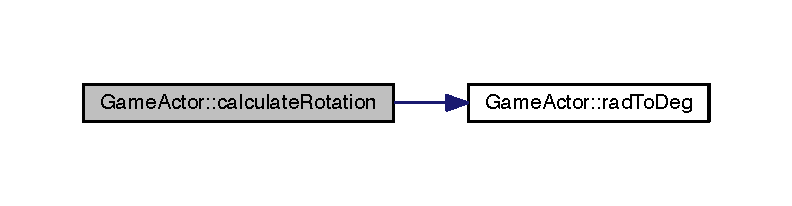
\includegraphics[width=350pt]{class_game_actor_a9f520d6799654aefd20c7a73d6c00f12_cgraph}
\end{center}
\end{figure}


\hypertarget{class_game_actor_a168ddb4dda02a8dd734f35d61e325de9}{\index{Game\+Actor@{Game\+Actor}!deal\+Damage@{deal\+Damage}}
\index{deal\+Damage@{deal\+Damage}!Game\+Actor@{Game\+Actor}}
\subsubsection[{deal\+Damage}]{\setlength{\rightskip}{0pt plus 5cm}void Game\+Actor\+::deal\+Damage (
\begin{DoxyParamCaption}
\item[{int}]{damage}
\end{DoxyParamCaption}
)}}\label{class_game_actor_a168ddb4dda02a8dd734f35d61e325de9}
Deals a given amount of damage to this \hyperlink{class_game_actor}{Game\+Actor} and determines whether this kills it. 
\begin{DoxyParams}{Parameters}
{\em damage} & the amount of damage to deal \\
\hline
\end{DoxyParams}


Here is the call graph for this function\+:\nopagebreak
\begin{figure}[H]
\begin{center}
\leavevmode
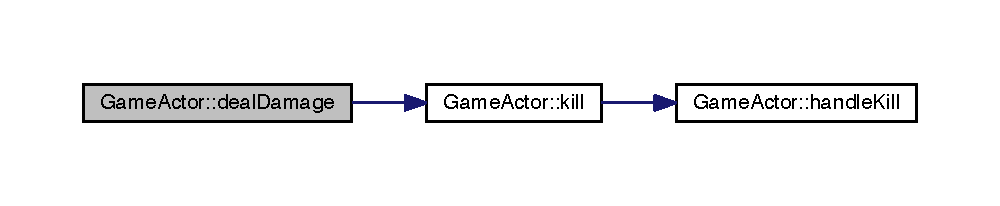
\includegraphics[width=350pt]{class_game_actor_a168ddb4dda02a8dd734f35d61e325de9_cgraph}
\end{center}
\end{figure}


\hypertarget{class_game_actor_aa50b1f399dc19a4dd62995641465cbd2}{\index{Game\+Actor@{Game\+Actor}!get\+Acceleration@{get\+Acceleration}}
\index{get\+Acceleration@{get\+Acceleration}!Game\+Actor@{Game\+Actor}}
\subsubsection[{get\+Acceleration}]{\setlength{\rightskip}{0pt plus 5cm}{\bf Vec3f} Game\+Actor\+::get\+Acceleration (
\begin{DoxyParamCaption}
{}
\end{DoxyParamCaption}
) const}}\label{class_game_actor_aa50b1f399dc19a4dd62995641465cbd2}
Determines the current acceleration. \begin{DoxyReturn}{Returns}
the current acceleration 
\end{DoxyReturn}
\hypertarget{class_game_actor_ad5717fb691f64dbfd6d05d8ab62a0e44}{\index{Game\+Actor@{Game\+Actor}!get\+Actors@{get\+Actors}}
\index{get\+Actors@{get\+Actors}!Game\+Actor@{Game\+Actor}}
\subsubsection[{get\+Actors}]{\setlength{\rightskip}{0pt plus 5cm}vector$<$ {\bf Game\+Actor} $\ast$ $>$ $\ast$ Game\+Actor\+::get\+Actors (
\begin{DoxyParamCaption}
{}
\end{DoxyParamCaption}
) const}}\label{class_game_actor_ad5717fb691f64dbfd6d05d8ab62a0e44}
Returns the \hyperlink{class_game_actor}{Game\+Actor} list of this \hyperlink{class_game_actor}{Game\+Actor}. \begin{DoxyReturn}{Returns}
the \hyperlink{class_game_actor}{Game\+Actor} list of this \hyperlink{class_game_actor}{Game\+Actor} 
\end{DoxyReturn}
\hypertarget{class_game_actor_a46068d92a30316a1bc86b3812fd255ce}{\index{Game\+Actor@{Game\+Actor}!get\+Distance@{get\+Distance}}
\index{get\+Distance@{get\+Distance}!Game\+Actor@{Game\+Actor}}
\subsubsection[{get\+Distance}]{\setlength{\rightskip}{0pt plus 5cm}float Game\+Actor\+::get\+Distance (
\begin{DoxyParamCaption}
\item[{{\bf Game\+Actor} \&}]{to}
\end{DoxyParamCaption}
) const}}\label{class_game_actor_a46068d92a30316a1bc86b3812fd255ce}
Determines the distance between this instance of \hyperlink{class_game_actor}{Game\+Actor} and a given one. 
\begin{DoxyParams}{Parameters}
{\em to} & the other \hyperlink{class_game_actor}{Game\+Actor} \\
\hline
\end{DoxyParams}
\begin{DoxyReturn}{Returns}
the distance to the given \hyperlink{class_game_actor}{Game\+Actor} 
\end{DoxyReturn}


Here is the call graph for this function\+:\nopagebreak
\begin{figure}[H]
\begin{center}
\leavevmode
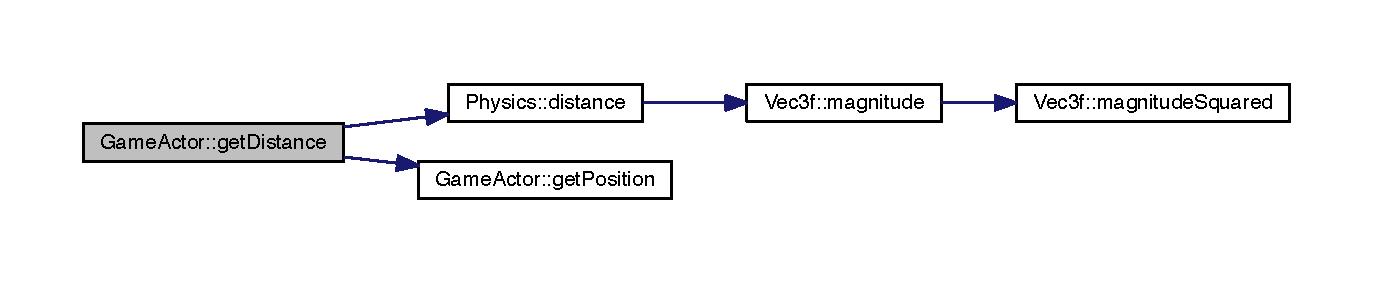
\includegraphics[width=350pt]{class_game_actor_a46068d92a30316a1bc86b3812fd255ce_cgraph}
\end{center}
\end{figure}


\hypertarget{class_game_actor_a34e8fa1fcd5febba5f9c92817a24583d}{\index{Game\+Actor@{Game\+Actor}!get\+Field@{get\+Field}}
\index{get\+Field@{get\+Field}!Game\+Actor@{Game\+Actor}}
\subsubsection[{get\+Field}]{\setlength{\rightskip}{0pt plus 5cm}{\bf Game\+Field} $\ast$ Game\+Actor\+::get\+Field (
\begin{DoxyParamCaption}
{}
\end{DoxyParamCaption}
) const}}\label{class_game_actor_a34e8fa1fcd5febba5f9c92817a24583d}
Returns the \hyperlink{class_game_field}{Game\+Field} of this \hyperlink{class_game_actor}{Game\+Actor}. \begin{DoxyReturn}{Returns}
the field 
\end{DoxyReturn}
\hypertarget{class_game_actor_a7fafd913a7b0f93d66f7335c8e8417f9}{\index{Game\+Actor@{Game\+Actor}!get\+G@{get\+G}}
\index{get\+G@{get\+G}!Game\+Actor@{Game\+Actor}}
\subsubsection[{get\+G}]{\setlength{\rightskip}{0pt plus 5cm}float Game\+Actor\+::get\+G (
\begin{DoxyParamCaption}
{}
\end{DoxyParamCaption}
) const}}\label{class_game_actor_a7fafd913a7b0f93d66f7335c8e8417f9}
Determines the current gravitational force \begin{DoxyReturn}{Returns}
the current gravitational force 
\end{DoxyReturn}
\hypertarget{class_game_actor_adb2e41937471e0f7377a188f399684cf}{\index{Game\+Actor@{Game\+Actor}!get\+Gravitation\+Range@{get\+Gravitation\+Range}}
\index{get\+Gravitation\+Range@{get\+Gravitation\+Range}!Game\+Actor@{Game\+Actor}}
\subsubsection[{get\+Gravitation\+Range}]{\setlength{\rightskip}{0pt plus 5cm}float Game\+Actor\+::get\+Gravitation\+Range (
\begin{DoxyParamCaption}
{}
\end{DoxyParamCaption}
) const}}\label{class_game_actor_adb2e41937471e0f7377a188f399684cf}
Determines the current gravitational range \begin{DoxyReturn}{Returns}
the current gravitational range 
\end{DoxyReturn}
\hypertarget{class_game_actor_a0e29a446b3247da54893ef12faa9eaaa}{\index{Game\+Actor@{Game\+Actor}!get\+Health@{get\+Health}}
\index{get\+Health@{get\+Health}!Game\+Actor@{Game\+Actor}}
\subsubsection[{get\+Health}]{\setlength{\rightskip}{0pt plus 5cm}int Game\+Actor\+::get\+Health (
\begin{DoxyParamCaption}
{}
\end{DoxyParamCaption}
) const}}\label{class_game_actor_a0e29a446b3247da54893ef12faa9eaaa}
Determines the current amount of health. \begin{DoxyReturn}{Returns}
the current health 
\end{DoxyReturn}
\hypertarget{class_game_actor_a64691c7e8f9d2d528d06323284a1d40c}{\index{Game\+Actor@{Game\+Actor}!get\+Identifier@{get\+Identifier}}
\index{get\+Identifier@{get\+Identifier}!Game\+Actor@{Game\+Actor}}
\subsubsection[{get\+Identifier}]{\setlength{\rightskip}{0pt plus 5cm}int Game\+Actor\+::get\+Identifier (
\begin{DoxyParamCaption}
{}
\end{DoxyParamCaption}
) const}}\label{class_game_actor_a64691c7e8f9d2d528d06323284a1d40c}
Determines the current identifier \begin{DoxyReturn}{Returns}
the current identifier 
\end{DoxyReturn}
\hypertarget{class_game_actor_ac19034996d2c622f4f2fd5870d43c9cd}{\index{Game\+Actor@{Game\+Actor}!get\+Mass@{get\+Mass}}
\index{get\+Mass@{get\+Mass}!Game\+Actor@{Game\+Actor}}
\subsubsection[{get\+Mass}]{\setlength{\rightskip}{0pt plus 5cm}float Game\+Actor\+::get\+Mass (
\begin{DoxyParamCaption}
{}
\end{DoxyParamCaption}
) const}}\label{class_game_actor_ac19034996d2c622f4f2fd5870d43c9cd}
Determines the current mass \begin{DoxyReturn}{Returns}
the current mass 
\end{DoxyReturn}
\hypertarget{class_game_actor_a13cec4e211c56989b4ef58ead7c31e17}{\index{Game\+Actor@{Game\+Actor}!get\+Max\+Speed@{get\+Max\+Speed}}
\index{get\+Max\+Speed@{get\+Max\+Speed}!Game\+Actor@{Game\+Actor}}
\subsubsection[{get\+Max\+Speed}]{\setlength{\rightskip}{0pt plus 5cm}float Game\+Actor\+::get\+Max\+Speed (
\begin{DoxyParamCaption}
{}
\end{DoxyParamCaption}
) const}}\label{class_game_actor_a13cec4e211c56989b4ef58ead7c31e17}
Determines the maximum speed. \begin{DoxyReturn}{Returns}
the maximum speed 
\end{DoxyReturn}
\hypertarget{class_game_actor_a8a0ca1b6866225d66df2381649bdc601}{\index{Game\+Actor@{Game\+Actor}!get\+Position@{get\+Position}}
\index{get\+Position@{get\+Position}!Game\+Actor@{Game\+Actor}}
\subsubsection[{get\+Position}]{\setlength{\rightskip}{0pt plus 5cm}{\bf Vec3f} Game\+Actor\+::get\+Position (
\begin{DoxyParamCaption}
{}
\end{DoxyParamCaption}
) const}}\label{class_game_actor_a8a0ca1b6866225d66df2381649bdc601}
Determines the current position \begin{DoxyReturn}{Returns}
the current position 
\end{DoxyReturn}
\hypertarget{class_game_actor_a1f624837eac0fe9fe80bcb54cfe8b1cf}{\index{Game\+Actor@{Game\+Actor}!get\+Velocity@{get\+Velocity}}
\index{get\+Velocity@{get\+Velocity}!Game\+Actor@{Game\+Actor}}
\subsubsection[{get\+Velocity}]{\setlength{\rightskip}{0pt plus 5cm}{\bf Vec3f} Game\+Actor\+::get\+Velocity (
\begin{DoxyParamCaption}
{}
\end{DoxyParamCaption}
) const}}\label{class_game_actor_a1f624837eac0fe9fe80bcb54cfe8b1cf}
Determines the current velocity. \begin{DoxyReturn}{Returns}
the current velocity 
\end{DoxyReturn}
\hypertarget{class_game_actor_ae63b522db0d88f56e3c7a8cfb60d31a6}{\index{Game\+Actor@{Game\+Actor}!get\+View@{get\+View}}
\index{get\+View@{get\+View}!Game\+Actor@{Game\+Actor}}
\subsubsection[{get\+View}]{\setlength{\rightskip}{0pt plus 5cm}{\bf Game\+Actor\+View} $\ast$ Game\+Actor\+::get\+View (
\begin{DoxyParamCaption}
{}
\end{DoxyParamCaption}
) const\hspace{0.3cm}{\ttfamily [virtual]}}}\label{class_game_actor_ae63b522db0d88f56e3c7a8cfb60d31a6}
Creates and returns a \hyperlink{class_game_actor_view}{Game\+Actor\+View} of this instance of \hyperlink{class_game_actor}{Game\+Actor}. \begin{DoxyReturn}{Returns}
the \hyperlink{class_game_actor_view}{Game\+Actor\+View} for this \hyperlink{class_game_actor}{Game\+Actor} 
\end{DoxyReturn}


Reimplemented in \hyperlink{class_spacecraft_ada8aff4825d826f3b8ab6ef3b4430529}{Spacecraft}, \hyperlink{class_laser_af00728fe7cabd4f63cb5ce66f4c50e86}{Laser}, \hyperlink{class_missile_a4ff3f60f70f5b4f8cf8ab3f0f6f509b6}{Missile}, \hyperlink{class_asteroid_a267c313e8759ca6091455616cc6c40f1}{Asteroid}, \hyperlink{class_planet_a60f36a3e87d89c4467e3ee2854906a09}{Planet}, \hyperlink{class_power_up_a7e5b4f541e42f88c41d9f04faba4cc53}{Power\+Up}, \hyperlink{class_scrap_a68649c3864eb5b426df61a57114b10ff}{Scrap}, and \hyperlink{class_sun_ae5833ea5166cf6bcd48958d05d37670e}{Sun}.



Here is the call graph for this function\+:\nopagebreak
\begin{figure}[H]
\begin{center}
\leavevmode
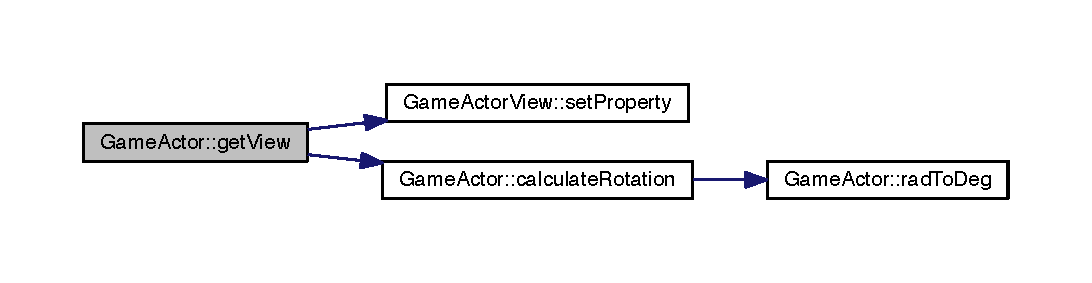
\includegraphics[width=350pt]{class_game_actor_ae63b522db0d88f56e3c7a8cfb60d31a6_cgraph}
\end{center}
\end{figure}


\hypertarget{class_game_actor_aba8cfb1004bf6fc17681cd595b706ada}{\index{Game\+Actor@{Game\+Actor}!handle\+Collision@{handle\+Collision}}
\index{handle\+Collision@{handle\+Collision}!Game\+Actor@{Game\+Actor}}
\subsubsection[{handle\+Collision}]{\setlength{\rightskip}{0pt plus 5cm}void Game\+Actor\+::handle\+Collision (
\begin{DoxyParamCaption}
\item[{{\bf Game\+Actor} \&}]{other}
\end{DoxyParamCaption}
)\hspace{0.3cm}{\ttfamily [virtual]}}}\label{class_game_actor_aba8cfb1004bf6fc17681cd595b706ada}
Determines what will happen if this \hyperlink{class_game_actor}{Game\+Actor} collides with another instance of \hyperlink{class_game_actor}{Game\+Actor}. 
\begin{DoxyParams}{Parameters}
{\em other} & the \hyperlink{class_game_actor}{Game\+Actor} colliding with this one \\
\hline
\end{DoxyParams}


Reimplemented in \hyperlink{class_spacecraft_a52608575fde91a502be1621b348884ec}{Spacecraft}, \hyperlink{class_laser_a6c26eb024fd0ae01920c299d1af2679d}{Laser}, \hyperlink{class_missile_a08f4b7e58d9382c46263677ac57c1efe}{Missile}, \hyperlink{class_aim_missile_aedbbc65c9b383913d3a401bfba40cd4e}{Aim\+Missile}, \hyperlink{class_asteroid_ada68cafcbb9e41c90f3e372de1a4b0ba}{Asteroid}, \hyperlink{class_planet_a9dd66b259905d35fa4233bd469662627}{Planet}, \hyperlink{class_power_up_adcd75e162366c12a062b915413ffff7a}{Power\+Up}, \hyperlink{class_scrap_a6db3dbd17f6d653c17d3f17dfcd448c5}{Scrap}, and \hyperlink{class_sun_a62d7b6c5a6089f29fc669240952a7362}{Sun}.

\hypertarget{class_game_actor_a00cdd692fae4de9fb4ce6b2748754744}{\index{Game\+Actor@{Game\+Actor}!handle\+Kill@{handle\+Kill}}
\index{handle\+Kill@{handle\+Kill}!Game\+Actor@{Game\+Actor}}
\subsubsection[{handle\+Kill}]{\setlength{\rightskip}{0pt plus 5cm}void Game\+Actor\+::handle\+Kill (
\begin{DoxyParamCaption}
{}
\end{DoxyParamCaption}
)\hspace{0.3cm}{\ttfamily [virtual]}}}\label{class_game_actor_a00cdd692fae4de9fb4ce6b2748754744}
Determines what will happen if this \hyperlink{class_game_actor}{Game\+Actor} is killed. 

Reimplemented in \hyperlink{class_spacecraft_a4609f3428987bc61e490519a8d1b9ccb}{Spacecraft}, and \hyperlink{class_planet_aa2932c76f46038b77b427c08167018cc}{Planet}.

\hypertarget{class_game_actor_a3ac80ca433821d22e545285c04cf38a1}{\index{Game\+Actor@{Game\+Actor}!is\+Killed@{is\+Killed}}
\index{is\+Killed@{is\+Killed}!Game\+Actor@{Game\+Actor}}
\subsubsection[{is\+Killed}]{\setlength{\rightskip}{0pt plus 5cm}bool Game\+Actor\+::is\+Killed (
\begin{DoxyParamCaption}
{}
\end{DoxyParamCaption}
)}}\label{class_game_actor_a3ac80ca433821d22e545285c04cf38a1}
Determines whether this \hyperlink{class_game_actor}{Game\+Actor} is killed or not. \begin{DoxyReturn}{Returns}
true if this \hyperlink{class_game_actor}{Game\+Actor} is killed, false otherwise 
\end{DoxyReturn}
\hypertarget{class_game_actor_a633b34eb69ad05477fd1d5b5de3c17b8}{\index{Game\+Actor@{Game\+Actor}!kill@{kill}}
\index{kill@{kill}!Game\+Actor@{Game\+Actor}}
\subsubsection[{kill}]{\setlength{\rightskip}{0pt plus 5cm}void Game\+Actor\+::kill (
\begin{DoxyParamCaption}
{}
\end{DoxyParamCaption}
)}}\label{class_game_actor_a633b34eb69ad05477fd1d5b5de3c17b8}
Marks this \hyperlink{class_game_actor}{Game\+Actor} as killed and triggers kill handling. 

Here is the call graph for this function\+:\nopagebreak
\begin{figure}[H]
\begin{center}
\leavevmode
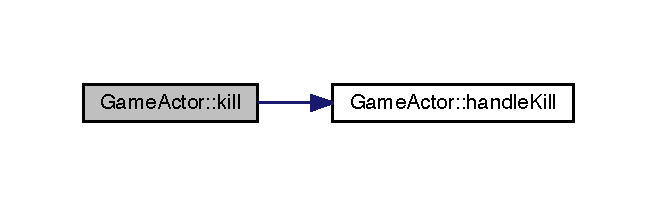
\includegraphics[width=315pt]{class_game_actor_a633b34eb69ad05477fd1d5b5de3c17b8_cgraph}
\end{center}
\end{figure}


\hypertarget{class_game_actor_a806e4306d891e32c4e06b961cbf11702}{\index{Game\+Actor@{Game\+Actor}!operator=@{operator=}}
\index{operator=@{operator=}!Game\+Actor@{Game\+Actor}}
\subsubsection[{operator=}]{\setlength{\rightskip}{0pt plus 5cm}{\bf Game\+Actor} \& Game\+Actor\+::operator= (
\begin{DoxyParamCaption}
\item[{const {\bf Game\+Actor} \&}]{right}
\end{DoxyParamCaption}
)}}\label{class_game_actor_a806e4306d891e32c4e06b961cbf11702}
Assigns a given \hyperlink{class_game_actor}{Game\+Actor} this one. \begin{DoxyReturn}{Returns}
this \hyperlink{class_game_actor}{Game\+Actor} after assignment 
\end{DoxyReturn}
\hypertarget{class_game_actor_a6052cc4a43b18dc72103a5a1abc521c2}{\index{Game\+Actor@{Game\+Actor}!operator==@{operator==}}
\index{operator==@{operator==}!Game\+Actor@{Game\+Actor}}
\subsubsection[{operator==}]{\setlength{\rightskip}{0pt plus 5cm}bool Game\+Actor\+::operator== (
\begin{DoxyParamCaption}
\item[{{\bf Game\+Actor} \&}]{right}
\end{DoxyParamCaption}
)}}\label{class_game_actor_a6052cc4a43b18dc72103a5a1abc521c2}
Determines whether to Game\+Actors are the same, in other words, whether they point to the same memory address. Other comparisons would be illogical since all vector based attributes of Game\+Actors could only be compared to a predestined degree of accuracy. \begin{DoxyReturn}{Returns}
true if both Game\+Actors are the same, false otherwise 
\end{DoxyReturn}
\hypertarget{class_game_actor_aee1a09ea167d0cb5d7c2e9c381611405}{\index{Game\+Actor@{Game\+Actor}!rad\+To\+Deg@{rad\+To\+Deg}}
\index{rad\+To\+Deg@{rad\+To\+Deg}!Game\+Actor@{Game\+Actor}}
\subsubsection[{rad\+To\+Deg}]{\setlength{\rightskip}{0pt plus 5cm}float Game\+Actor\+::rad\+To\+Deg (
\begin{DoxyParamCaption}
\item[{float}]{radians}
\end{DoxyParamCaption}
) const\hspace{0.3cm}{\ttfamily [protected]}}}\label{class_game_actor_aee1a09ea167d0cb5d7c2e9c381611405}
Converts a given value in radians to degrees. 
\begin{DoxyParams}{Parameters}
{\em radians} & the radians value to convert \\
\hline
\end{DoxyParams}
\begin{DoxyReturn}{Returns}
the converted vlue 
\end{DoxyReturn}
\hypertarget{class_game_actor_ab8d3dd08796d2459f7d377b143197bf0}{\index{Game\+Actor@{Game\+Actor}!set\+Actors@{set\+Actors}}
\index{set\+Actors@{set\+Actors}!Game\+Actor@{Game\+Actor}}
\subsubsection[{set\+Actors}]{\setlength{\rightskip}{0pt plus 5cm}void Game\+Actor\+::set\+Actors (
\begin{DoxyParamCaption}
\item[{vector$<$ {\bf Game\+Actor} $\ast$ $>$ $\ast$}]{actors}
\end{DoxyParamCaption}
)}}\label{class_game_actor_ab8d3dd08796d2459f7d377b143197bf0}
Replaces the \hyperlink{class_game_actor}{Game\+Actor} list of this instance with a given list. 
\begin{DoxyParams}{Parameters}
{\em actors} & a list (vector) with Game\+Actors which will interact with this instance of \hyperlink{class_game_actor}{Game\+Actor} \\
\hline
\end{DoxyParams}
\hypertarget{class_game_actor_af3fbd8b984fdd0df93cc4c6f342caa5e}{\index{Game\+Actor@{Game\+Actor}!set\+G@{set\+G}}
\index{set\+G@{set\+G}!Game\+Actor@{Game\+Actor}}
\subsubsection[{set\+G}]{\setlength{\rightskip}{0pt plus 5cm}void Game\+Actor\+::set\+G (
\begin{DoxyParamCaption}
\item[{float}]{g}
\end{DoxyParamCaption}
)}}\label{class_game_actor_af3fbd8b984fdd0df93cc4c6f342caa5e}
Sets the gravitational force to a given value. 
\begin{DoxyParams}{Parameters}
{\em g} & the value to set \\
\hline
\end{DoxyParams}
\hypertarget{class_game_actor_ace7f2c9f95ac3c39acbb88a3c31240b4}{\index{Game\+Actor@{Game\+Actor}!set\+Health@{set\+Health}}
\index{set\+Health@{set\+Health}!Game\+Actor@{Game\+Actor}}
\subsubsection[{set\+Health}]{\setlength{\rightskip}{0pt plus 5cm}void Game\+Actor\+::set\+Health (
\begin{DoxyParamCaption}
\item[{int}]{health}
\end{DoxyParamCaption}
)}}\label{class_game_actor_ace7f2c9f95ac3c39acbb88a3c31240b4}
Sets the to a given value. 
\begin{DoxyParams}{Parameters}
{\em g} & the value to set \\
\hline
\end{DoxyParams}
\hypertarget{class_game_actor_a33f79600c44e3372a23c3ca2ee880704}{\index{Game\+Actor@{Game\+Actor}!set\+Max\+Speed@{set\+Max\+Speed}}
\index{set\+Max\+Speed@{set\+Max\+Speed}!Game\+Actor@{Game\+Actor}}
\subsubsection[{set\+Max\+Speed}]{\setlength{\rightskip}{0pt plus 5cm}void Game\+Actor\+::set\+Max\+Speed (
\begin{DoxyParamCaption}
\item[{float}]{max\+Speed}
\end{DoxyParamCaption}
)}}\label{class_game_actor_a33f79600c44e3372a23c3ca2ee880704}
Sets the maximum speed to a given value. 
\begin{DoxyParams}{Parameters}
{\em g} & the value to set \\
\hline
\end{DoxyParams}
\hypertarget{class_game_actor_a10bb2f607937d5b376c4e0d9bc304d1c}{\index{Game\+Actor@{Game\+Actor}!to\+String@{to\+String}}
\index{to\+String@{to\+String}!Game\+Actor@{Game\+Actor}}
\subsubsection[{to\+String}]{\setlength{\rightskip}{0pt plus 5cm}std\+::string Game\+Actor\+::to\+String (
\begin{DoxyParamCaption}
{}
\end{DoxyParamCaption}
) const\hspace{0.3cm}{\ttfamily [virtual]}}}\label{class_game_actor_a10bb2f607937d5b376c4e0d9bc304d1c}
Creates and returns a string representation of this \hyperlink{class_game_actor}{Game\+Actor}. \begin{DoxyReturn}{Returns}
string representation of this \hyperlink{class_game_actor}{Game\+Actor} 
\end{DoxyReturn}


Here is the call graph for this function\+:\nopagebreak
\begin{figure}[H]
\begin{center}
\leavevmode
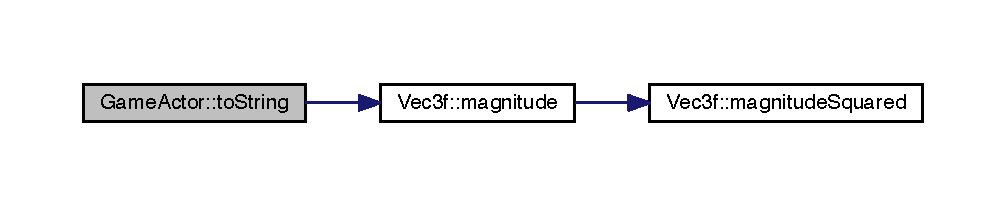
\includegraphics[width=350pt]{class_game_actor_a10bb2f607937d5b376c4e0d9bc304d1c_cgraph}
\end{center}
\end{figure}


\hypertarget{class_game_actor_ab70229c740251fb7c4222bf579c59393}{\index{Game\+Actor@{Game\+Actor}!update@{update}}
\index{update@{update}!Game\+Actor@{Game\+Actor}}
\subsubsection[{update}]{\setlength{\rightskip}{0pt plus 5cm}void Game\+Actor\+::update (
\begin{DoxyParamCaption}
{}
\end{DoxyParamCaption}
)\hspace{0.3cm}{\ttfamily [virtual]}}}\label{class_game_actor_ab70229c740251fb7c4222bf579c59393}
Updates the position and velocity of this \hyperlink{class_game_actor}{Game\+Actor}. With this implementation Game\+Actors will be bounced off the game field borders. 

Reimplemented in \hyperlink{class_projectile_ac41ad56034b53e739619fabbd5e49652}{Projectile}, \hyperlink{class_aim_missile_a2723e6b87d30aa722b795e955a04ddfd}{Aim\+Missile}, \hyperlink{class_planet_a56f440c725e00a3b27e4fbd8da87813d}{Planet}, and \hyperlink{class_sun_ae6c8bd44775ae0207c59908b4abdb7f5}{Sun}.



Here is the call graph for this function\+:\nopagebreak
\begin{figure}[H]
\begin{center}
\leavevmode
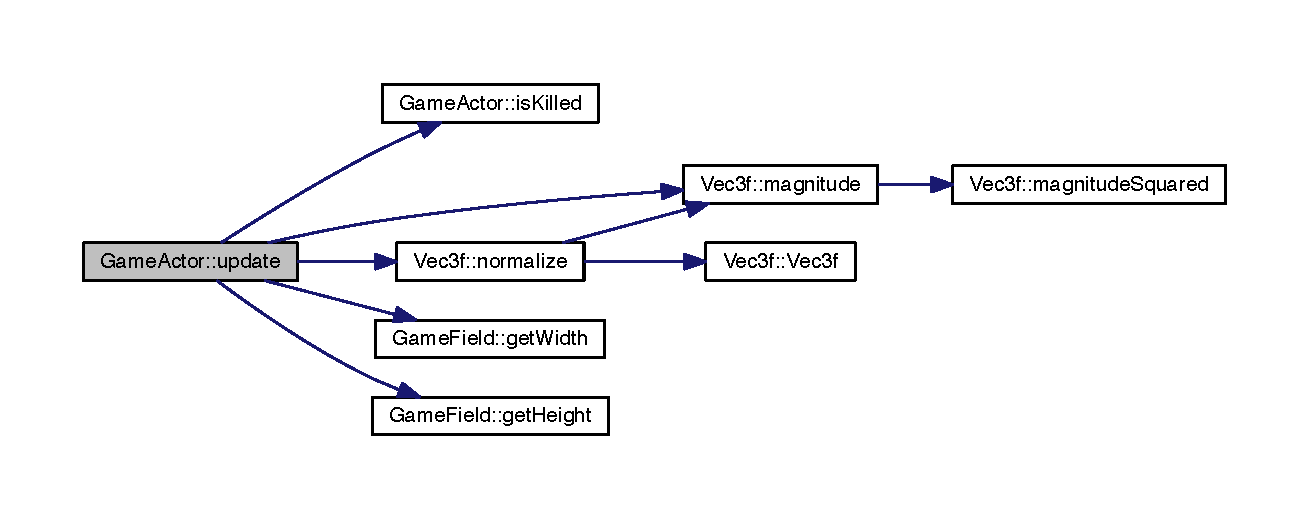
\includegraphics[width=350pt]{class_game_actor_ab70229c740251fb7c4222bf579c59393_cgraph}
\end{center}
\end{figure}


\hypertarget{class_game_actor_a2d3b93df5edf86dea7d65ab7dac0e3f7}{\index{Game\+Actor@{Game\+Actor}!update\+All@{update\+All}}
\index{update\+All@{update\+All}!Game\+Actor@{Game\+Actor}}
\subsubsection[{update\+All}]{\setlength{\rightskip}{0pt plus 5cm}void Game\+Actor\+::update\+All (
\begin{DoxyParamCaption}
{}
\end{DoxyParamCaption}
)\hspace{0.3cm}{\ttfamily [virtual]}}}\label{class_game_actor_a2d3b93df5edf86dea7d65ab7dac0e3f7}
Checks for collisions with other Game\+Actors, triggers collision handling as well as the calculation and application of the gravitational force towards all other Game\+Actors. 

Here is the call graph for this function\+:\nopagebreak
\begin{figure}[H]
\begin{center}
\leavevmode
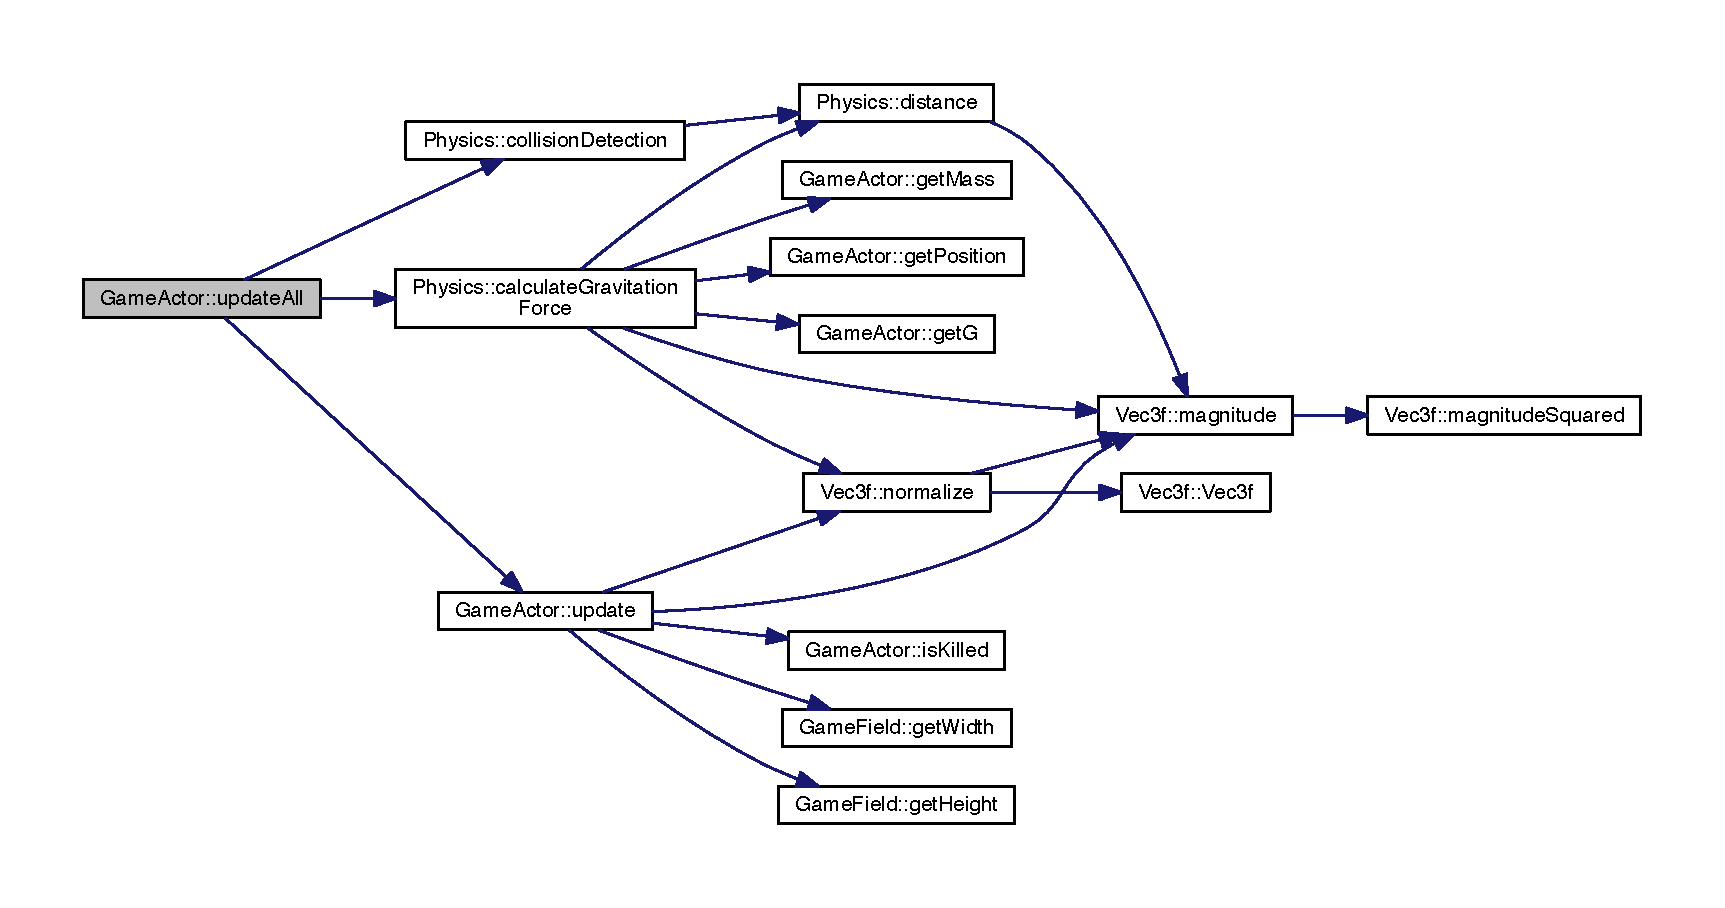
\includegraphics[width=350pt]{class_game_actor_a2d3b93df5edf86dea7d65ab7dac0e3f7_cgraph}
\end{center}
\end{figure}




\subsection{Member Data Documentation}
\hypertarget{class_game_actor_aa62fdbdad09045bcd6f3a150c3a0038b}{\index{Game\+Actor@{Game\+Actor}!acceleration@{acceleration}}
\index{acceleration@{acceleration}!Game\+Actor@{Game\+Actor}}
\subsubsection[{acceleration}]{\setlength{\rightskip}{0pt plus 5cm}{\bf Vec3f} Game\+Actor\+::acceleration\hspace{0.3cm}{\ttfamily [protected]}}}\label{class_game_actor_aa62fdbdad09045bcd6f3a150c3a0038b}
Acceleration is the force, that will be applied to the Game\+Actors velocity per frame. \hypertarget{class_game_actor_a2405618d895f5143b42ae9e94d20e693}{\index{Game\+Actor@{Game\+Actor}!actors@{actors}}
\index{actors@{actors}!Game\+Actor@{Game\+Actor}}
\subsubsection[{actors}]{\setlength{\rightskip}{0pt plus 5cm}vector$<${\bf Game\+Actor}$\ast$$>$$\ast$ Game\+Actor\+::actors\hspace{0.3cm}{\ttfamily [protected]}}}\label{class_game_actor_a2405618d895f5143b42ae9e94d20e693}
A list (vector) of all other Game\+Actors \hypertarget{class_game_actor_a0224fbc502abd6b7579787aa234332d5}{\index{Game\+Actor@{Game\+Actor}!field@{field}}
\index{field@{field}!Game\+Actor@{Game\+Actor}}
\subsubsection[{field}]{\setlength{\rightskip}{0pt plus 5cm}{\bf Game\+Field}$\ast$ Game\+Actor\+::field\hspace{0.3cm}{\ttfamily [protected]}}}\label{class_game_actor_a0224fbc502abd6b7579787aa234332d5}
The game area. \hypertarget{class_game_actor_a42ed4bef0d99cf053ff9a025c86d34d3}{\index{Game\+Actor@{Game\+Actor}!g@{g}}
\index{g@{g}!Game\+Actor@{Game\+Actor}}
\subsubsection[{g}]{\setlength{\rightskip}{0pt plus 5cm}float Game\+Actor\+::g\hspace{0.3cm}{\ttfamily [protected]}}}\label{class_game_actor_a42ed4bef0d99cf053ff9a025c86d34d3}
The gravitational force or pull of this \hyperlink{class_game_actor}{Game\+Actor}. \hypertarget{class_game_actor_a9c0ba51b08a3e617d9629c0ee8d309f2}{\index{Game\+Actor@{Game\+Actor}!gravitation\+Range@{gravitation\+Range}}
\index{gravitation\+Range@{gravitation\+Range}!Game\+Actor@{Game\+Actor}}
\subsubsection[{gravitation\+Range}]{\setlength{\rightskip}{0pt plus 5cm}float Game\+Actor\+::gravitation\+Range\hspace{0.3cm}{\ttfamily [protected]}}}\label{class_game_actor_a9c0ba51b08a3e617d9629c0ee8d309f2}
The range over which this \hyperlink{class_game_actor}{Game\+Actor} can apply its own gravitational pull to other Game\+Actors. \hypertarget{class_game_actor_a5d402a953140585fb7cc3f8a3a24a2a4}{\index{Game\+Actor@{Game\+Actor}!health@{health}}
\index{health@{health}!Game\+Actor@{Game\+Actor}}
\subsubsection[{health}]{\setlength{\rightskip}{0pt plus 5cm}int Game\+Actor\+::health\hspace{0.3cm}{\ttfamily [protected]}}}\label{class_game_actor_a5d402a953140585fb7cc3f8a3a24a2a4}
The health points of this \hyperlink{class_game_actor}{Game\+Actor}, 0 indicating a dead \hyperlink{class_game_actor}{Game\+Actor} and -\/1 indicating an immortal \hyperlink{class_game_actor}{Game\+Actor}. \hypertarget{class_game_actor_a07be525e1e463a4f437dba30f0173b6c}{\index{Game\+Actor@{Game\+Actor}!id@{id}}
\index{id@{id}!Game\+Actor@{Game\+Actor}}
\subsubsection[{id}]{\setlength{\rightskip}{0pt plus 5cm}int Game\+Actor\+::id = 0\hspace{0.3cm}{\ttfamily [static]}, {\ttfamily [protected]}}}\label{class_game_actor_a07be525e1e463a4f437dba30f0173b6c}
A global counter representing the number of all Game\+Actors. It will be increased, whenever a new \hyperlink{class_game_actor}{Game\+Actor} is instantiated. \hypertarget{class_game_actor_af0f1723601974c63c9df8a60a6ce7da7}{\index{Game\+Actor@{Game\+Actor}!identifier@{identifier}}
\index{identifier@{identifier}!Game\+Actor@{Game\+Actor}}
\subsubsection[{identifier}]{\setlength{\rightskip}{0pt plus 5cm}int Game\+Actor\+::identifier\hspace{0.3cm}{\ttfamily [protected]}}}\label{class_game_actor_af0f1723601974c63c9df8a60a6ce7da7}
The identifier of this \hyperlink{class_game_actor}{Game\+Actor}. Equals the id field at the time of instantiation of this very \hyperlink{class_game_actor}{Game\+Actor}. \hypertarget{class_game_actor_a7f8bd5ef8278fda5db77a372d8bb6bb9}{\index{Game\+Actor@{Game\+Actor}!killed@{killed}}
\index{killed@{killed}!Game\+Actor@{Game\+Actor}}
\subsubsection[{killed}]{\setlength{\rightskip}{0pt plus 5cm}bool Game\+Actor\+::killed\hspace{0.3cm}{\ttfamily [protected]}}}\label{class_game_actor_a7f8bd5ef8278fda5db77a372d8bb6bb9}
Defines whether this \hyperlink{class_game_actor}{Game\+Actor} counts as killed or not. This will have implications on both the effects of other Game\+Actors and the updating process. \hypertarget{class_game_actor_a2111233f4f0216db4d172d5088ebeed4}{\index{Game\+Actor@{Game\+Actor}!mass@{mass}}
\index{mass@{mass}!Game\+Actor@{Game\+Actor}}
\subsubsection[{mass}]{\setlength{\rightskip}{0pt plus 5cm}float Game\+Actor\+::mass\hspace{0.3cm}{\ttfamily [protected]}}}\label{class_game_actor_a2111233f4f0216db4d172d5088ebeed4}
The mass of the \hyperlink{class_game_actor}{Game\+Actor}, but actually a factor in relation to a preset normal mass. \hypertarget{class_game_actor_a15b6abd006c52b21c569932f8b484eb0}{\index{Game\+Actor@{Game\+Actor}!max\+Speed@{max\+Speed}}
\index{max\+Speed@{max\+Speed}!Game\+Actor@{Game\+Actor}}
\subsubsection[{max\+Speed}]{\setlength{\rightskip}{0pt plus 5cm}float Game\+Actor\+::max\+Speed\hspace{0.3cm}{\ttfamily [protected]}}}\label{class_game_actor_a15b6abd006c52b21c569932f8b484eb0}
The maximum speed this \hyperlink{class_game_actor}{Game\+Actor} can acquire. \hypertarget{class_game_actor_aefed3c91bf32ad388d86657b3bb9ddfa}{\index{Game\+Actor@{Game\+Actor}!position@{position}}
\index{position@{position}!Game\+Actor@{Game\+Actor}}
\subsubsection[{position}]{\setlength{\rightskip}{0pt plus 5cm}{\bf Vec3f} Game\+Actor\+::position\hspace{0.3cm}{\ttfamily [protected]}}}\label{class_game_actor_aefed3c91bf32ad388d86657b3bb9ddfa}
The current position of the \hyperlink{class_game_actor}{Game\+Actor} in a 3-\/dimensional Cartesian space. \hypertarget{class_game_actor_a95518bf01411eafe983df8815e8682d1}{\index{Game\+Actor@{Game\+Actor}!velocity@{velocity}}
\index{velocity@{velocity}!Game\+Actor@{Game\+Actor}}
\subsubsection[{velocity}]{\setlength{\rightskip}{0pt plus 5cm}{\bf Vec3f} Game\+Actor\+::velocity\hspace{0.3cm}{\ttfamily [protected]}}}\label{class_game_actor_a95518bf01411eafe983df8815e8682d1}
Velocity is the actual direction and speed for this \hyperlink{class_game_actor}{Game\+Actor}. 

The documentation for this class was generated from the following files\+:\begin{DoxyCompactItemize}
\item 
src/headers/\hyperlink{_game_actor_8h}{Game\+Actor.\+h}\item 
src/\hyperlink{_game_actor_8cpp}{Game\+Actor.\+cpp}\end{DoxyCompactItemize}

\hypertarget{class_game_actor_view}{\section{Game\+Actor\+View Class Reference}
\label{class_game_actor_view}\index{Game\+Actor\+View@{Game\+Actor\+View}}
}


{\ttfamily \#include $<$Game\+Actor\+View.\+h$>$}

\subsection*{Public Member Functions}
\begin{DoxyCompactItemize}
\item 
\hyperlink{class_game_actor_view_ac364ad4b8b84afeb3646afb2c9595315}{Game\+Actor\+View} ()
\item 
\hyperlink{class_game_actor_view_a701bf0bc7aa6ef90cd96afbcdca731da}{Game\+Actor\+View} (string the\+Qml\+Path)
\item 
string \hyperlink{class_game_actor_view_a5a796c75c6205f0f7874a3bce97cfba8}{get\+Qml\+Path} () const 
\item 
void \hyperlink{class_game_actor_view_a89d3c6c159128714e6780c4fda51fdcd}{set\+Property} (string key, string value)
\item 
void \hyperlink{class_game_actor_view_aa1911219122fef24d4953b9aebdfba21}{set\+Property} (string key, float value)
\item 
void \hyperlink{class_game_actor_view_ae7a1149056fffae502fa92b7a83ed026}{set\+Property} (string key, bool value)
\item 
void \hyperlink{class_game_actor_view_aa783426287a1ec0f3fd54aeffbcc9407}{set\+Property} (string key, int value)
\item 
string \hyperlink{class_game_actor_view_a36c37691a940aa339beb5aebec818933}{get\+Propterty} (string key)
\item 
map$<$ string, string $>$ \hyperlink{class_game_actor_view_a1c08b8b6229640a6312e088bf173c2a8}{get\+Properties} () const 
\item 
string \hyperlink{class_game_actor_view_a7aacc01fec85433fcefd43663b48a763}{to\+String} () const 
\item 
void \hyperlink{class_game_actor_view_a36cb82690cbaf53296a1b24d32a36140}{from\+String} (string serialized)
\end{DoxyCompactItemize}


\subsection{Constructor \& Destructor Documentation}
\hypertarget{class_game_actor_view_ac364ad4b8b84afeb3646afb2c9595315}{\index{Game\+Actor\+View@{Game\+Actor\+View}!Game\+Actor\+View@{Game\+Actor\+View}}
\index{Game\+Actor\+View@{Game\+Actor\+View}!Game\+Actor\+View@{Game\+Actor\+View}}
\subsubsection[{Game\+Actor\+View}]{\setlength{\rightskip}{0pt plus 5cm}Game\+Actor\+View\+::\+Game\+Actor\+View (
\begin{DoxyParamCaption}
{}
\end{DoxyParamCaption}
)}}\label{class_game_actor_view_ac364ad4b8b84afeb3646afb2c9595315}
\hypertarget{class_game_actor_view_a701bf0bc7aa6ef90cd96afbcdca731da}{\index{Game\+Actor\+View@{Game\+Actor\+View}!Game\+Actor\+View@{Game\+Actor\+View}}
\index{Game\+Actor\+View@{Game\+Actor\+View}!Game\+Actor\+View@{Game\+Actor\+View}}
\subsubsection[{Game\+Actor\+View}]{\setlength{\rightskip}{0pt plus 5cm}Game\+Actor\+View\+::\+Game\+Actor\+View (
\begin{DoxyParamCaption}
\item[{string}]{the\+Qml\+Path}
\end{DoxyParamCaption}
)}}\label{class_game_actor_view_a701bf0bc7aa6ef90cd96afbcdca731da}


\subsection{Member Function Documentation}
\hypertarget{class_game_actor_view_a36cb82690cbaf53296a1b24d32a36140}{\index{Game\+Actor\+View@{Game\+Actor\+View}!from\+String@{from\+String}}
\index{from\+String@{from\+String}!Game\+Actor\+View@{Game\+Actor\+View}}
\subsubsection[{from\+String}]{\setlength{\rightskip}{0pt plus 5cm}void Game\+Actor\+View\+::from\+String (
\begin{DoxyParamCaption}
\item[{string}]{serialized}
\end{DoxyParamCaption}
)}}\label{class_game_actor_view_a36cb82690cbaf53296a1b24d32a36140}


Here is the call graph for this function\+:\nopagebreak
\begin{figure}[H]
\begin{center}
\leavevmode
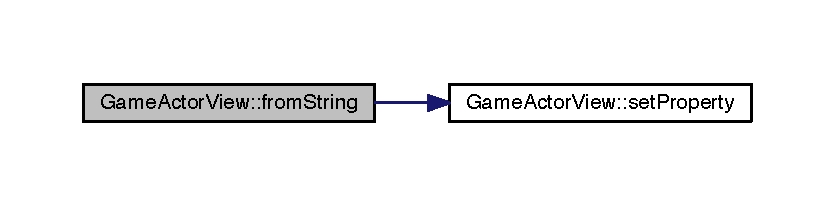
\includegraphics[width=350pt]{class_game_actor_view_a36cb82690cbaf53296a1b24d32a36140_cgraph}
\end{center}
\end{figure}


\hypertarget{class_game_actor_view_a1c08b8b6229640a6312e088bf173c2a8}{\index{Game\+Actor\+View@{Game\+Actor\+View}!get\+Properties@{get\+Properties}}
\index{get\+Properties@{get\+Properties}!Game\+Actor\+View@{Game\+Actor\+View}}
\subsubsection[{get\+Properties}]{\setlength{\rightskip}{0pt plus 5cm}map$<$ string, string $>$ Game\+Actor\+View\+::get\+Properties (
\begin{DoxyParamCaption}
{}
\end{DoxyParamCaption}
) const}}\label{class_game_actor_view_a1c08b8b6229640a6312e088bf173c2a8}
\hypertarget{class_game_actor_view_a36c37691a940aa339beb5aebec818933}{\index{Game\+Actor\+View@{Game\+Actor\+View}!get\+Propterty@{get\+Propterty}}
\index{get\+Propterty@{get\+Propterty}!Game\+Actor\+View@{Game\+Actor\+View}}
\subsubsection[{get\+Propterty}]{\setlength{\rightskip}{0pt plus 5cm}string Game\+Actor\+View\+::get\+Propterty (
\begin{DoxyParamCaption}
\item[{string}]{key}
\end{DoxyParamCaption}
)}}\label{class_game_actor_view_a36c37691a940aa339beb5aebec818933}
\hypertarget{class_game_actor_view_a5a796c75c6205f0f7874a3bce97cfba8}{\index{Game\+Actor\+View@{Game\+Actor\+View}!get\+Qml\+Path@{get\+Qml\+Path}}
\index{get\+Qml\+Path@{get\+Qml\+Path}!Game\+Actor\+View@{Game\+Actor\+View}}
\subsubsection[{get\+Qml\+Path}]{\setlength{\rightskip}{0pt plus 5cm}string Game\+Actor\+View\+::get\+Qml\+Path (
\begin{DoxyParamCaption}
{}
\end{DoxyParamCaption}
) const}}\label{class_game_actor_view_a5a796c75c6205f0f7874a3bce97cfba8}
\hypertarget{class_game_actor_view_a89d3c6c159128714e6780c4fda51fdcd}{\index{Game\+Actor\+View@{Game\+Actor\+View}!set\+Property@{set\+Property}}
\index{set\+Property@{set\+Property}!Game\+Actor\+View@{Game\+Actor\+View}}
\subsubsection[{set\+Property}]{\setlength{\rightskip}{0pt plus 5cm}void Game\+Actor\+View\+::set\+Property (
\begin{DoxyParamCaption}
\item[{string}]{key, }
\item[{string}]{value}
\end{DoxyParamCaption}
)}}\label{class_game_actor_view_a89d3c6c159128714e6780c4fda51fdcd}
\hypertarget{class_game_actor_view_aa1911219122fef24d4953b9aebdfba21}{\index{Game\+Actor\+View@{Game\+Actor\+View}!set\+Property@{set\+Property}}
\index{set\+Property@{set\+Property}!Game\+Actor\+View@{Game\+Actor\+View}}
\subsubsection[{set\+Property}]{\setlength{\rightskip}{0pt plus 5cm}void Game\+Actor\+View\+::set\+Property (
\begin{DoxyParamCaption}
\item[{string}]{key, }
\item[{float}]{value}
\end{DoxyParamCaption}
)}}\label{class_game_actor_view_aa1911219122fef24d4953b9aebdfba21}


Here is the call graph for this function\+:\nopagebreak
\begin{figure}[H]
\begin{center}
\leavevmode
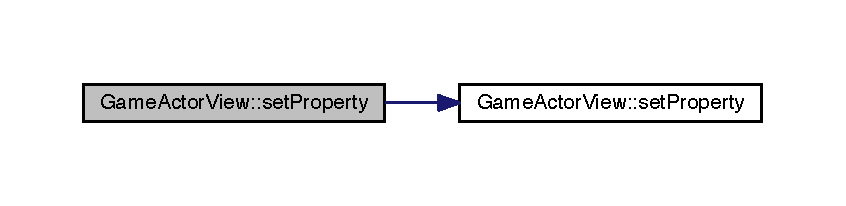
\includegraphics[width=350pt]{class_game_actor_view_aa1911219122fef24d4953b9aebdfba21_cgraph}
\end{center}
\end{figure}


\hypertarget{class_game_actor_view_ae7a1149056fffae502fa92b7a83ed026}{\index{Game\+Actor\+View@{Game\+Actor\+View}!set\+Property@{set\+Property}}
\index{set\+Property@{set\+Property}!Game\+Actor\+View@{Game\+Actor\+View}}
\subsubsection[{set\+Property}]{\setlength{\rightskip}{0pt plus 5cm}void Game\+Actor\+View\+::set\+Property (
\begin{DoxyParamCaption}
\item[{string}]{key, }
\item[{bool}]{value}
\end{DoxyParamCaption}
)}}\label{class_game_actor_view_ae7a1149056fffae502fa92b7a83ed026}


Here is the call graph for this function\+:\nopagebreak
\begin{figure}[H]
\begin{center}
\leavevmode
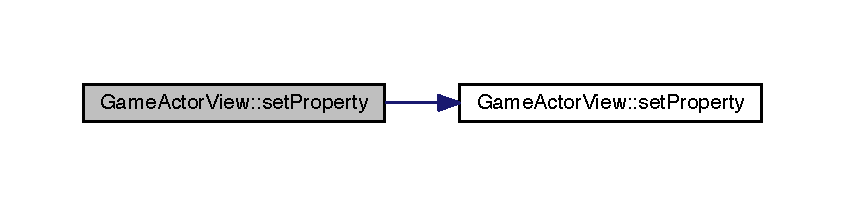
\includegraphics[width=350pt]{class_game_actor_view_ae7a1149056fffae502fa92b7a83ed026_cgraph}
\end{center}
\end{figure}


\hypertarget{class_game_actor_view_aa783426287a1ec0f3fd54aeffbcc9407}{\index{Game\+Actor\+View@{Game\+Actor\+View}!set\+Property@{set\+Property}}
\index{set\+Property@{set\+Property}!Game\+Actor\+View@{Game\+Actor\+View}}
\subsubsection[{set\+Property}]{\setlength{\rightskip}{0pt plus 5cm}void Game\+Actor\+View\+::set\+Property (
\begin{DoxyParamCaption}
\item[{string}]{key, }
\item[{int}]{value}
\end{DoxyParamCaption}
)}}\label{class_game_actor_view_aa783426287a1ec0f3fd54aeffbcc9407}


Here is the call graph for this function\+:\nopagebreak
\begin{figure}[H]
\begin{center}
\leavevmode
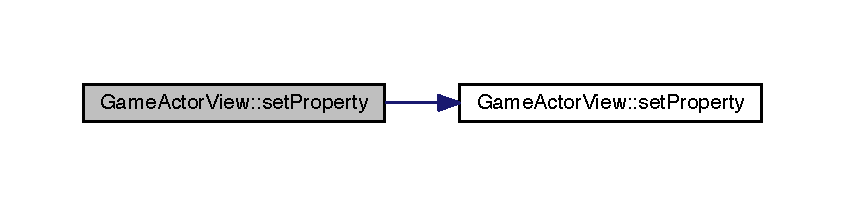
\includegraphics[width=350pt]{class_game_actor_view_aa783426287a1ec0f3fd54aeffbcc9407_cgraph}
\end{center}
\end{figure}


\hypertarget{class_game_actor_view_a7aacc01fec85433fcefd43663b48a763}{\index{Game\+Actor\+View@{Game\+Actor\+View}!to\+String@{to\+String}}
\index{to\+String@{to\+String}!Game\+Actor\+View@{Game\+Actor\+View}}
\subsubsection[{to\+String}]{\setlength{\rightskip}{0pt plus 5cm}string Game\+Actor\+View\+::to\+String (
\begin{DoxyParamCaption}
{}
\end{DoxyParamCaption}
) const}}\label{class_game_actor_view_a7aacc01fec85433fcefd43663b48a763}


Here is the call graph for this function\+:\nopagebreak
\begin{figure}[H]
\begin{center}
\leavevmode
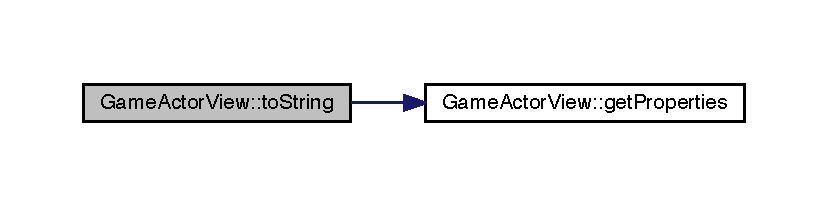
\includegraphics[width=350pt]{class_game_actor_view_a7aacc01fec85433fcefd43663b48a763_cgraph}
\end{center}
\end{figure}




The documentation for this class was generated from the following files\+:\begin{DoxyCompactItemize}
\item 
src/headers/\hyperlink{_game_actor_view_8h}{Game\+Actor\+View.\+h}\item 
src/\hyperlink{_game_actor_view_8cpp}{Game\+Actor\+View.\+cpp}\end{DoxyCompactItemize}

\hypertarget{class_game_field}{\section{Game\+Field Class Reference}
\label{class_game_field}\index{Game\+Field@{Game\+Field}}
}


{\ttfamily \#include $<$Game\+Field.\+h$>$}

\subsection*{Public Member Functions}
\begin{DoxyCompactItemize}
\item 
\hyperlink{class_game_field_ad86d2092617bbda4da40b8d6a14f892d}{Game\+Field} ()
\item 
\hyperlink{class_game_field_a76c70cb4fb981de20995e4486c727a47}{Game\+Field} (int, int)
\item 
void \hyperlink{class_game_field_a29d50e60f4728dc6945c95acf1086514}{set\+Width} (int)
\item 
void \hyperlink{class_game_field_a389c3c6dd873493066a725b673e3fc87}{set\+Height} (int)
\item 
int \hyperlink{class_game_field_a7a551f2b02f8446903c636aa41c16341}{get\+Height} () const 
\item 
int \hyperlink{class_game_field_a4e64e71ba15b89734e6bbed36b8936a2}{get\+Width} () const 
\end{DoxyCompactItemize}


\subsection{Constructor \& Destructor Documentation}
\hypertarget{class_game_field_ad86d2092617bbda4da40b8d6a14f892d}{\index{Game\+Field@{Game\+Field}!Game\+Field@{Game\+Field}}
\index{Game\+Field@{Game\+Field}!Game\+Field@{Game\+Field}}
\subsubsection[{Game\+Field}]{\setlength{\rightskip}{0pt plus 5cm}Game\+Field\+::\+Game\+Field (
\begin{DoxyParamCaption}
{}
\end{DoxyParamCaption}
)}}\label{class_game_field_ad86d2092617bbda4da40b8d6a14f892d}
\hypertarget{class_game_field_a76c70cb4fb981de20995e4486c727a47}{\index{Game\+Field@{Game\+Field}!Game\+Field@{Game\+Field}}
\index{Game\+Field@{Game\+Field}!Game\+Field@{Game\+Field}}
\subsubsection[{Game\+Field}]{\setlength{\rightskip}{0pt plus 5cm}Game\+Field\+::\+Game\+Field (
\begin{DoxyParamCaption}
\item[{int}]{width, }
\item[{int}]{height}
\end{DoxyParamCaption}
)}}\label{class_game_field_a76c70cb4fb981de20995e4486c727a47}


\subsection{Member Function Documentation}
\hypertarget{class_game_field_a7a551f2b02f8446903c636aa41c16341}{\index{Game\+Field@{Game\+Field}!get\+Height@{get\+Height}}
\index{get\+Height@{get\+Height}!Game\+Field@{Game\+Field}}
\subsubsection[{get\+Height}]{\setlength{\rightskip}{0pt plus 5cm}int Game\+Field\+::get\+Height (
\begin{DoxyParamCaption}
{}
\end{DoxyParamCaption}
) const}}\label{class_game_field_a7a551f2b02f8446903c636aa41c16341}
\hypertarget{class_game_field_a4e64e71ba15b89734e6bbed36b8936a2}{\index{Game\+Field@{Game\+Field}!get\+Width@{get\+Width}}
\index{get\+Width@{get\+Width}!Game\+Field@{Game\+Field}}
\subsubsection[{get\+Width}]{\setlength{\rightskip}{0pt plus 5cm}int Game\+Field\+::get\+Width (
\begin{DoxyParamCaption}
{}
\end{DoxyParamCaption}
) const}}\label{class_game_field_a4e64e71ba15b89734e6bbed36b8936a2}
\hypertarget{class_game_field_a389c3c6dd873493066a725b673e3fc87}{\index{Game\+Field@{Game\+Field}!set\+Height@{set\+Height}}
\index{set\+Height@{set\+Height}!Game\+Field@{Game\+Field}}
\subsubsection[{set\+Height}]{\setlength{\rightskip}{0pt plus 5cm}void Game\+Field\+::set\+Height (
\begin{DoxyParamCaption}
\item[{int}]{height}
\end{DoxyParamCaption}
)}}\label{class_game_field_a389c3c6dd873493066a725b673e3fc87}
\hypertarget{class_game_field_a29d50e60f4728dc6945c95acf1086514}{\index{Game\+Field@{Game\+Field}!set\+Width@{set\+Width}}
\index{set\+Width@{set\+Width}!Game\+Field@{Game\+Field}}
\subsubsection[{set\+Width}]{\setlength{\rightskip}{0pt plus 5cm}void Game\+Field\+::set\+Width (
\begin{DoxyParamCaption}
\item[{int}]{width}
\end{DoxyParamCaption}
)}}\label{class_game_field_a29d50e60f4728dc6945c95acf1086514}


The documentation for this class was generated from the following files\+:\begin{DoxyCompactItemize}
\item 
src/headers/\hyperlink{_game_field_8h}{Game\+Field.\+h}\item 
src/\hyperlink{_game_field_8cpp}{Game\+Field.\+cpp}\end{DoxyCompactItemize}

\hypertarget{class_game_generator}{\section{Game\+Generator Class Reference}
\label{class_game_generator}\index{Game\+Generator@{Game\+Generator}}
}


{\ttfamily \#include $<$Game\+Generator.\+h$>$}



Inheritance diagram for Game\+Generator\+:\nopagebreak
\begin{figure}[H]
\begin{center}
\leavevmode
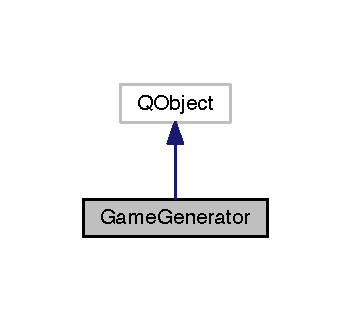
\includegraphics[width=168pt]{class_game_generator__inherit__graph}
\end{center}
\end{figure}


Collaboration diagram for Game\+Generator\+:\nopagebreak
\begin{figure}[H]
\begin{center}
\leavevmode
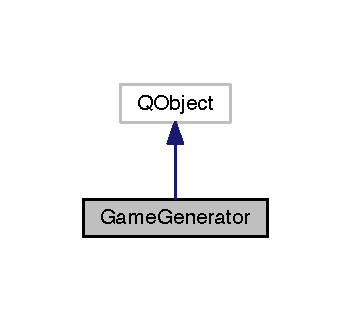
\includegraphics[width=168pt]{class_game_generator__coll__graph}
\end{center}
\end{figure}
\subsection*{Public Member Functions}
\begin{DoxyCompactItemize}
\item 
\hyperlink{class_game_generator_a6d2a4240e25126da4a6646835f7b1a28}{Game\+Generator} (Q\+Object $\ast$parent=0)
\item 
\hyperlink{class_game_generator_ae50a42e8512131b500b37db65d2bb4ce}{Game\+Generator} (\hyperlink{class_gravitron_settings}{Gravitron\+Settings} $\ast$settings, \hyperlink{class_game_field}{Game\+Field} $\ast$field)
\item 
\hyperlink{class_game_generator_a1912c6f1efadf83c48e5a73a95ab464e}{Game\+Generator} (\hyperlink{class_gravitron_settings}{Gravitron\+Settings} $\ast$settings, \hyperlink{class_game_field}{Game\+Field} $\ast$field, \hyperlink{class_tcp_server}{Tcp\+Server} $\ast$server)
\item 
\hyperlink{class_game_generator_afacbbddbe5e11a62ec6f59df93d384fe}{Game\+Generator} (const \hyperlink{class_game_generator}{Game\+Generator} \&original)
\item 
\hyperlink{class_game_generator_a2376a3b5b93faf7c1c592cb70297fd7c}{$\sim$\+Game\+Generator} ()
\item 
void \hyperlink{class_game_generator_a13f50521a481baafdae183e44d410977}{generate\+Game} (\hyperlink{class_game_loop}{Game\+Loop} $\ast$g)
\item 
\hyperlink{class_game_actor}{Game\+Actor} $\ast$ \hyperlink{class_game_generator_acd01e34ebb3653724b238c5e1fedc3ad}{generate\+New\+Power\+Up} (\hyperlink{class_vec3f}{Vec3f} position)
\item 
\hyperlink{class_game_actor}{Game\+Actor} $\ast$ \hyperlink{class_game_generator_a8b44d635c748aaf630afb41ad21a368e}{generate\+New\+Scrap} (\hyperlink{class_vec3f}{Vec3f} position)
\end{DoxyCompactItemize}


\subsection{Constructor \& Destructor Documentation}
\hypertarget{class_game_generator_a6d2a4240e25126da4a6646835f7b1a28}{\index{Game\+Generator@{Game\+Generator}!Game\+Generator@{Game\+Generator}}
\index{Game\+Generator@{Game\+Generator}!Game\+Generator@{Game\+Generator}}
\subsubsection[{Game\+Generator}]{\setlength{\rightskip}{0pt plus 5cm}Game\+Generator\+::\+Game\+Generator (
\begin{DoxyParamCaption}
\item[{Q\+Object $\ast$}]{parent = {\ttfamily 0}}
\end{DoxyParamCaption}
)\hspace{0.3cm}{\ttfamily [explicit]}}}\label{class_game_generator_a6d2a4240e25126da4a6646835f7b1a28}
\hypertarget{class_game_generator_ae50a42e8512131b500b37db65d2bb4ce}{\index{Game\+Generator@{Game\+Generator}!Game\+Generator@{Game\+Generator}}
\index{Game\+Generator@{Game\+Generator}!Game\+Generator@{Game\+Generator}}
\subsubsection[{Game\+Generator}]{\setlength{\rightskip}{0pt plus 5cm}Game\+Generator\+::\+Game\+Generator (
\begin{DoxyParamCaption}
\item[{{\bf Gravitron\+Settings} $\ast$}]{settings, }
\item[{{\bf Game\+Field} $\ast$}]{field}
\end{DoxyParamCaption}
)}}\label{class_game_generator_ae50a42e8512131b500b37db65d2bb4ce}
\hypertarget{class_game_generator_a1912c6f1efadf83c48e5a73a95ab464e}{\index{Game\+Generator@{Game\+Generator}!Game\+Generator@{Game\+Generator}}
\index{Game\+Generator@{Game\+Generator}!Game\+Generator@{Game\+Generator}}
\subsubsection[{Game\+Generator}]{\setlength{\rightskip}{0pt plus 5cm}Game\+Generator\+::\+Game\+Generator (
\begin{DoxyParamCaption}
\item[{{\bf Gravitron\+Settings} $\ast$}]{settings, }
\item[{{\bf Game\+Field} $\ast$}]{field, }
\item[{{\bf Tcp\+Server} $\ast$}]{server}
\end{DoxyParamCaption}
)}}\label{class_game_generator_a1912c6f1efadf83c48e5a73a95ab464e}
\hypertarget{class_game_generator_afacbbddbe5e11a62ec6f59df93d384fe}{\index{Game\+Generator@{Game\+Generator}!Game\+Generator@{Game\+Generator}}
\index{Game\+Generator@{Game\+Generator}!Game\+Generator@{Game\+Generator}}
\subsubsection[{Game\+Generator}]{\setlength{\rightskip}{0pt plus 5cm}Game\+Generator\+::\+Game\+Generator (
\begin{DoxyParamCaption}
\item[{const {\bf Game\+Generator} \&}]{original}
\end{DoxyParamCaption}
)}}\label{class_game_generator_afacbbddbe5e11a62ec6f59df93d384fe}
\hypertarget{class_game_generator_a2376a3b5b93faf7c1c592cb70297fd7c}{\index{Game\+Generator@{Game\+Generator}!````~Game\+Generator@{$\sim$\+Game\+Generator}}
\index{````~Game\+Generator@{$\sim$\+Game\+Generator}!Game\+Generator@{Game\+Generator}}
\subsubsection[{$\sim$\+Game\+Generator}]{\setlength{\rightskip}{0pt plus 5cm}Game\+Generator\+::$\sim$\+Game\+Generator (
\begin{DoxyParamCaption}
{}
\end{DoxyParamCaption}
)}}\label{class_game_generator_a2376a3b5b93faf7c1c592cb70297fd7c}


\subsection{Member Function Documentation}
\hypertarget{class_game_generator_a13f50521a481baafdae183e44d410977}{\index{Game\+Generator@{Game\+Generator}!generate\+Game@{generate\+Game}}
\index{generate\+Game@{generate\+Game}!Game\+Generator@{Game\+Generator}}
\subsubsection[{generate\+Game}]{\setlength{\rightskip}{0pt plus 5cm}void Game\+Generator\+::generate\+Game (
\begin{DoxyParamCaption}
\item[{{\bf Game\+Loop} $\ast$}]{g}
\end{DoxyParamCaption}
)}}\label{class_game_generator_a13f50521a481baafdae183e44d410977}


Here is the call graph for this function\+:\nopagebreak
\begin{figure}[H]
\begin{center}
\leavevmode
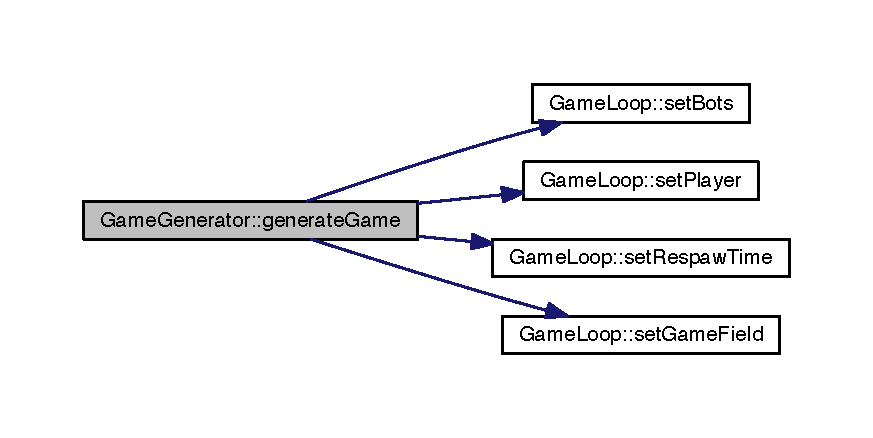
\includegraphics[width=350pt]{class_game_generator_a13f50521a481baafdae183e44d410977_cgraph}
\end{center}
\end{figure}


\hypertarget{class_game_generator_acd01e34ebb3653724b238c5e1fedc3ad}{\index{Game\+Generator@{Game\+Generator}!generate\+New\+Power\+Up@{generate\+New\+Power\+Up}}
\index{generate\+New\+Power\+Up@{generate\+New\+Power\+Up}!Game\+Generator@{Game\+Generator}}
\subsubsection[{generate\+New\+Power\+Up}]{\setlength{\rightskip}{0pt plus 5cm}{\bf Game\+Actor} $\ast$ Game\+Generator\+::generate\+New\+Power\+Up (
\begin{DoxyParamCaption}
\item[{{\bf Vec3f}}]{position}
\end{DoxyParamCaption}
)}}\label{class_game_generator_acd01e34ebb3653724b238c5e1fedc3ad}
\hypertarget{class_game_generator_a8b44d635c748aaf630afb41ad21a368e}{\index{Game\+Generator@{Game\+Generator}!generate\+New\+Scrap@{generate\+New\+Scrap}}
\index{generate\+New\+Scrap@{generate\+New\+Scrap}!Game\+Generator@{Game\+Generator}}
\subsubsection[{generate\+New\+Scrap}]{\setlength{\rightskip}{0pt plus 5cm}{\bf Game\+Actor} $\ast$ Game\+Generator\+::generate\+New\+Scrap (
\begin{DoxyParamCaption}
\item[{{\bf Vec3f}}]{position}
\end{DoxyParamCaption}
)}}\label{class_game_generator_a8b44d635c748aaf630afb41ad21a368e}


The documentation for this class was generated from the following files\+:\begin{DoxyCompactItemize}
\item 
src/headers/\hyperlink{_game_generator_8h}{Game\+Generator.\+h}\item 
src/\hyperlink{_game_generator_8cpp}{Game\+Generator.\+cpp}\end{DoxyCompactItemize}

\hypertarget{class_game_loop}{\section{Game\+Loop Class Reference}
\label{class_game_loop}\index{Game\+Loop@{Game\+Loop}}
}


{\ttfamily \#include $<$Game\+Loop.\+h$>$}



Inheritance diagram for Game\+Loop\+:\nopagebreak
\begin{figure}[H]
\begin{center}
\leavevmode
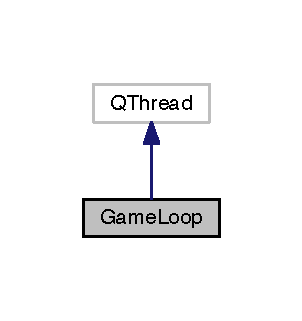
\includegraphics[width=145pt]{class_game_loop__inherit__graph}
\end{center}
\end{figure}


Collaboration diagram for Game\+Loop\+:\nopagebreak
\begin{figure}[H]
\begin{center}
\leavevmode
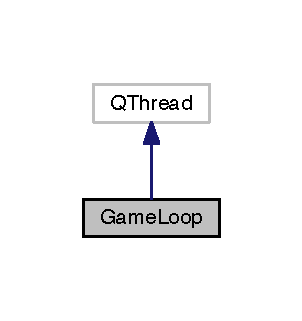
\includegraphics[width=145pt]{class_game_loop__coll__graph}
\end{center}
\end{figure}
\subsection*{Public Slots}
\begin{DoxyCompactItemize}
\item 
void \hyperlink{class_game_loop_a819f7585c0841dbad50444dc08312ae1}{run} ()
\end{DoxyCompactItemize}
\subsection*{Signals}
\begin{DoxyCompactItemize}
\item 
void \hyperlink{class_game_loop_ad5697eb532af7a8285f2a5b2173a1fb2}{render\+Object} (vector$<$ \hyperlink{class_game_actor_view}{Game\+Actor\+View} $\ast$ $>$ $\ast$views)
\item 
void \hyperlink{class_game_loop_a31966af3329677b02e4b9ac766835251}{send\+Viewlist} (Q\+String viewlist)
\item 
void \hyperlink{class_game_loop_a6e937ff7eddd17ee16157d757ec8d869}{active\+Weapon\+Game} (int weapon\+Number)
\item 
void \hyperlink{class_game_loop_a7b8774e746e18475abfd162b8c1ff1a8}{lifepoints} (int lifepoints)
\item 
void \hyperlink{class_game_loop_aadf44e47c371f83b0edda98ed5a4c96b}{background\+Pos} (float x, float y, float field\+Width, float field\+Height)
\item 
void \hyperlink{class_game_loop_a93c1aa53a02624ddd0078a67fe367fc7}{the\+Winner\+Is} (Q\+String winner\+Name)
\item 
void \hyperlink{class_game_loop_a357cac9658c9f6206d26c538fd7773ad}{frag\+Status} (int must, int have)
\end{DoxyCompactItemize}
\subsection*{Public Member Functions}
\begin{DoxyCompactItemize}
\item 
\hyperlink{class_game_loop_ae06492a249f44724b6781e414b282fbb}{Game\+Loop} (\hyperlink{class_game_generator}{Game\+Generator} g\+Generator)
\item 
virtual \hyperlink{class_game_loop_ae6c558d0d751a068dbafe2cae465ec1f}{$\sim$\+Game\+Loop} ()
\item 
void \hyperlink{class_game_loop_aef2bffc387feba32401fb222d2893213}{set\+Bots} (vector$<$ \hyperlink{class_a_i_player}{A\+I\+Player} $\ast$ $>$ bots)
\item 
void \hyperlink{class_game_loop_aa9cac681fffdcfde5df8b259409dd0ab}{set\+Player} (vector$<$ \hyperlink{class_player}{Player} $\ast$ $>$ player)
\item 
void \hyperlink{class_game_loop_a754c44ba0f01e81d411235d09e3296f5}{set\+Actors} (vector$<$ \hyperlink{class_game_actor}{Game\+Actor} $\ast$ $>$ \hyperlink{class_game_loop_a22d3c6823c5f67eccd389db6f5c2eb10}{actors})
\item 
void \hyperlink{class_game_loop_afa580dfac60d3a821ff1320c0da1cd56}{set\+Game\+Field} (\hyperlink{class_game_field}{Game\+Field} $\ast$new\+Field)
\item 
void \hyperlink{class_game_loop_ae32109f8170985968acce0525f71f015}{set\+Respaw\+Time} (int respawn\+Time)
\item 
void \hyperlink{class_game_loop_aee78756218e0fcf3ab73f4810c13dd0d}{stop} ()
\end{DoxyCompactItemize}
\subsection*{Public Attributes}
\begin{DoxyCompactItemize}
\item 
std\+::vector$<$ \hyperlink{class_game_actor}{Game\+Actor} $\ast$ $>$ \hyperlink{class_game_loop_a22d3c6823c5f67eccd389db6f5c2eb10}{actors}
\end{DoxyCompactItemize}


\subsection{Constructor \& Destructor Documentation}
\hypertarget{class_game_loop_ae06492a249f44724b6781e414b282fbb}{\index{Game\+Loop@{Game\+Loop}!Game\+Loop@{Game\+Loop}}
\index{Game\+Loop@{Game\+Loop}!Game\+Loop@{Game\+Loop}}
\subsubsection[{Game\+Loop}]{\setlength{\rightskip}{0pt plus 5cm}Game\+Loop\+::\+Game\+Loop (
\begin{DoxyParamCaption}
\item[{{\bf Game\+Generator}}]{g\+Generator}
\end{DoxyParamCaption}
)}}\label{class_game_loop_ae06492a249f44724b6781e414b282fbb}


Here is the call graph for this function\+:\nopagebreak
\begin{figure}[H]
\begin{center}
\leavevmode
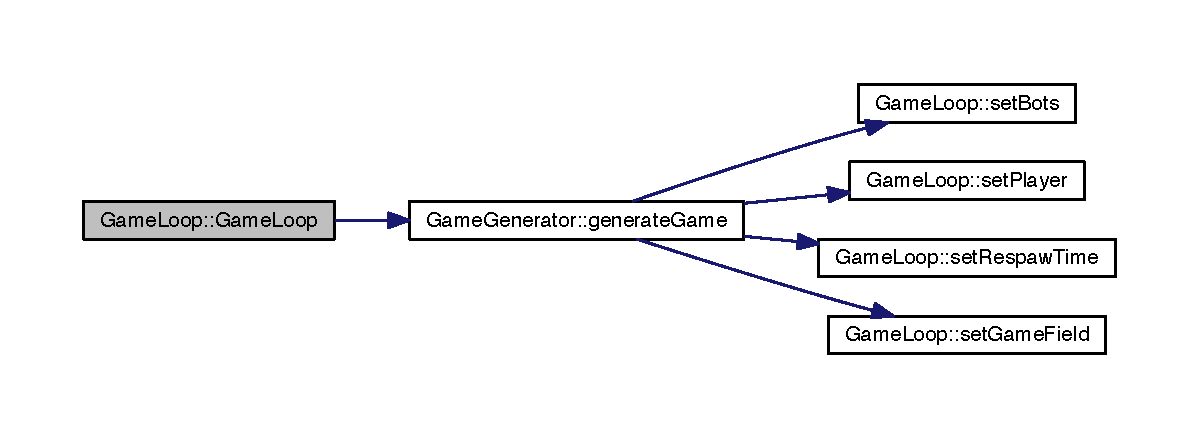
\includegraphics[width=350pt]{class_game_loop_ae06492a249f44724b6781e414b282fbb_cgraph}
\end{center}
\end{figure}


\hypertarget{class_game_loop_ae6c558d0d751a068dbafe2cae465ec1f}{\index{Game\+Loop@{Game\+Loop}!````~Game\+Loop@{$\sim$\+Game\+Loop}}
\index{````~Game\+Loop@{$\sim$\+Game\+Loop}!Game\+Loop@{Game\+Loop}}
\subsubsection[{$\sim$\+Game\+Loop}]{\setlength{\rightskip}{0pt plus 5cm}Game\+Loop\+::$\sim$\+Game\+Loop (
\begin{DoxyParamCaption}
{}
\end{DoxyParamCaption}
)\hspace{0.3cm}{\ttfamily [virtual]}}}\label{class_game_loop_ae6c558d0d751a068dbafe2cae465ec1f}


\subsection{Member Function Documentation}
\hypertarget{class_game_loop_a6e937ff7eddd17ee16157d757ec8d869}{\index{Game\+Loop@{Game\+Loop}!active\+Weapon\+Game@{active\+Weapon\+Game}}
\index{active\+Weapon\+Game@{active\+Weapon\+Game}!Game\+Loop@{Game\+Loop}}
\subsubsection[{active\+Weapon\+Game}]{\setlength{\rightskip}{0pt plus 5cm}void Game\+Loop\+::active\+Weapon\+Game (
\begin{DoxyParamCaption}
\item[{int}]{weapon\+Number}
\end{DoxyParamCaption}
)\hspace{0.3cm}{\ttfamily [signal]}}}\label{class_game_loop_a6e937ff7eddd17ee16157d757ec8d869}
\hypertarget{class_game_loop_aadf44e47c371f83b0edda98ed5a4c96b}{\index{Game\+Loop@{Game\+Loop}!background\+Pos@{background\+Pos}}
\index{background\+Pos@{background\+Pos}!Game\+Loop@{Game\+Loop}}
\subsubsection[{background\+Pos}]{\setlength{\rightskip}{0pt plus 5cm}void Game\+Loop\+::background\+Pos (
\begin{DoxyParamCaption}
\item[{float}]{x, }
\item[{float}]{y, }
\item[{float}]{field\+Width, }
\item[{float}]{field\+Height}
\end{DoxyParamCaption}
)\hspace{0.3cm}{\ttfamily [signal]}}}\label{class_game_loop_aadf44e47c371f83b0edda98ed5a4c96b}
\hypertarget{class_game_loop_a357cac9658c9f6206d26c538fd7773ad}{\index{Game\+Loop@{Game\+Loop}!frag\+Status@{frag\+Status}}
\index{frag\+Status@{frag\+Status}!Game\+Loop@{Game\+Loop}}
\subsubsection[{frag\+Status}]{\setlength{\rightskip}{0pt plus 5cm}void Game\+Loop\+::frag\+Status (
\begin{DoxyParamCaption}
\item[{int}]{must, }
\item[{int}]{have}
\end{DoxyParamCaption}
)\hspace{0.3cm}{\ttfamily [signal]}}}\label{class_game_loop_a357cac9658c9f6206d26c538fd7773ad}
\hypertarget{class_game_loop_a7b8774e746e18475abfd162b8c1ff1a8}{\index{Game\+Loop@{Game\+Loop}!lifepoints@{lifepoints}}
\index{lifepoints@{lifepoints}!Game\+Loop@{Game\+Loop}}
\subsubsection[{lifepoints}]{\setlength{\rightskip}{0pt plus 5cm}void Game\+Loop\+::lifepoints (
\begin{DoxyParamCaption}
\item[{int}]{lifepoints}
\end{DoxyParamCaption}
)\hspace{0.3cm}{\ttfamily [signal]}}}\label{class_game_loop_a7b8774e746e18475abfd162b8c1ff1a8}
\hypertarget{class_game_loop_ad5697eb532af7a8285f2a5b2173a1fb2}{\index{Game\+Loop@{Game\+Loop}!render\+Object@{render\+Object}}
\index{render\+Object@{render\+Object}!Game\+Loop@{Game\+Loop}}
\subsubsection[{render\+Object}]{\setlength{\rightskip}{0pt plus 5cm}void Game\+Loop\+::render\+Object (
\begin{DoxyParamCaption}
\item[{vector$<$ {\bf Game\+Actor\+View} $\ast$ $>$ $\ast$}]{views}
\end{DoxyParamCaption}
)\hspace{0.3cm}{\ttfamily [signal]}}}\label{class_game_loop_ad5697eb532af7a8285f2a5b2173a1fb2}
\hypertarget{class_game_loop_a819f7585c0841dbad50444dc08312ae1}{\index{Game\+Loop@{Game\+Loop}!run@{run}}
\index{run@{run}!Game\+Loop@{Game\+Loop}}
\subsubsection[{run}]{\setlength{\rightskip}{0pt plus 5cm}void Game\+Loop\+::run (
\begin{DoxyParamCaption}
{}
\end{DoxyParamCaption}
)\hspace{0.3cm}{\ttfamily [slot]}}}\label{class_game_loop_a819f7585c0841dbad50444dc08312ae1}
\hypertarget{class_game_loop_a31966af3329677b02e4b9ac766835251}{\index{Game\+Loop@{Game\+Loop}!send\+Viewlist@{send\+Viewlist}}
\index{send\+Viewlist@{send\+Viewlist}!Game\+Loop@{Game\+Loop}}
\subsubsection[{send\+Viewlist}]{\setlength{\rightskip}{0pt plus 5cm}void Game\+Loop\+::send\+Viewlist (
\begin{DoxyParamCaption}
\item[{Q\+String}]{viewlist}
\end{DoxyParamCaption}
)\hspace{0.3cm}{\ttfamily [signal]}}}\label{class_game_loop_a31966af3329677b02e4b9ac766835251}
\hypertarget{class_game_loop_a754c44ba0f01e81d411235d09e3296f5}{\index{Game\+Loop@{Game\+Loop}!set\+Actors@{set\+Actors}}
\index{set\+Actors@{set\+Actors}!Game\+Loop@{Game\+Loop}}
\subsubsection[{set\+Actors}]{\setlength{\rightskip}{0pt plus 5cm}void Game\+Loop\+::set\+Actors (
\begin{DoxyParamCaption}
\item[{vector$<$ {\bf Game\+Actor} $\ast$ $>$}]{actors}
\end{DoxyParamCaption}
)}}\label{class_game_loop_a754c44ba0f01e81d411235d09e3296f5}
\hypertarget{class_game_loop_aef2bffc387feba32401fb222d2893213}{\index{Game\+Loop@{Game\+Loop}!set\+Bots@{set\+Bots}}
\index{set\+Bots@{set\+Bots}!Game\+Loop@{Game\+Loop}}
\subsubsection[{set\+Bots}]{\setlength{\rightskip}{0pt plus 5cm}void Game\+Loop\+::set\+Bots (
\begin{DoxyParamCaption}
\item[{vector$<$ {\bf A\+I\+Player} $\ast$ $>$}]{bots}
\end{DoxyParamCaption}
)}}\label{class_game_loop_aef2bffc387feba32401fb222d2893213}
\hypertarget{class_game_loop_afa580dfac60d3a821ff1320c0da1cd56}{\index{Game\+Loop@{Game\+Loop}!set\+Game\+Field@{set\+Game\+Field}}
\index{set\+Game\+Field@{set\+Game\+Field}!Game\+Loop@{Game\+Loop}}
\subsubsection[{set\+Game\+Field}]{\setlength{\rightskip}{0pt plus 5cm}void Game\+Loop\+::set\+Game\+Field (
\begin{DoxyParamCaption}
\item[{{\bf Game\+Field} $\ast$}]{new\+Field}
\end{DoxyParamCaption}
)}}\label{class_game_loop_afa580dfac60d3a821ff1320c0da1cd56}
\hypertarget{class_game_loop_aa9cac681fffdcfde5df8b259409dd0ab}{\index{Game\+Loop@{Game\+Loop}!set\+Player@{set\+Player}}
\index{set\+Player@{set\+Player}!Game\+Loop@{Game\+Loop}}
\subsubsection[{set\+Player}]{\setlength{\rightskip}{0pt plus 5cm}void Game\+Loop\+::set\+Player (
\begin{DoxyParamCaption}
\item[{vector$<$ {\bf Player} $\ast$ $>$}]{player}
\end{DoxyParamCaption}
)}}\label{class_game_loop_aa9cac681fffdcfde5df8b259409dd0ab}
\hypertarget{class_game_loop_ae32109f8170985968acce0525f71f015}{\index{Game\+Loop@{Game\+Loop}!set\+Respaw\+Time@{set\+Respaw\+Time}}
\index{set\+Respaw\+Time@{set\+Respaw\+Time}!Game\+Loop@{Game\+Loop}}
\subsubsection[{set\+Respaw\+Time}]{\setlength{\rightskip}{0pt plus 5cm}void Game\+Loop\+::set\+Respaw\+Time (
\begin{DoxyParamCaption}
\item[{int}]{respawn\+Time}
\end{DoxyParamCaption}
)}}\label{class_game_loop_ae32109f8170985968acce0525f71f015}
\hypertarget{class_game_loop_aee78756218e0fcf3ab73f4810c13dd0d}{\index{Game\+Loop@{Game\+Loop}!stop@{stop}}
\index{stop@{stop}!Game\+Loop@{Game\+Loop}}
\subsubsection[{stop}]{\setlength{\rightskip}{0pt plus 5cm}void Game\+Loop\+::stop (
\begin{DoxyParamCaption}
{}
\end{DoxyParamCaption}
)}}\label{class_game_loop_aee78756218e0fcf3ab73f4810c13dd0d}
\hypertarget{class_game_loop_a93c1aa53a02624ddd0078a67fe367fc7}{\index{Game\+Loop@{Game\+Loop}!the\+Winner\+Is@{the\+Winner\+Is}}
\index{the\+Winner\+Is@{the\+Winner\+Is}!Game\+Loop@{Game\+Loop}}
\subsubsection[{the\+Winner\+Is}]{\setlength{\rightskip}{0pt plus 5cm}void Game\+Loop\+::the\+Winner\+Is (
\begin{DoxyParamCaption}
\item[{Q\+String}]{winner\+Name}
\end{DoxyParamCaption}
)\hspace{0.3cm}{\ttfamily [signal]}}}\label{class_game_loop_a93c1aa53a02624ddd0078a67fe367fc7}


\subsection{Member Data Documentation}
\hypertarget{class_game_loop_a22d3c6823c5f67eccd389db6f5c2eb10}{\index{Game\+Loop@{Game\+Loop}!actors@{actors}}
\index{actors@{actors}!Game\+Loop@{Game\+Loop}}
\subsubsection[{actors}]{\setlength{\rightskip}{0pt plus 5cm}std\+::vector$<${\bf Game\+Actor}$\ast$$>$ Game\+Loop\+::actors}}\label{class_game_loop_a22d3c6823c5f67eccd389db6f5c2eb10}


The documentation for this class was generated from the following files\+:\begin{DoxyCompactItemize}
\item 
src/headers/\hyperlink{_game_loop_8h}{Game\+Loop.\+h}\item 
src/\hyperlink{_game_loop_8cpp}{Game\+Loop.\+cpp}\end{DoxyCompactItemize}

\hypertarget{class_gravitron_difficulties}{\section{Gravitron\+Difficulties Class Reference}
\label{class_gravitron_difficulties}\index{Gravitron\+Difficulties@{Gravitron\+Difficulties}}
}


{\ttfamily \#include $<$Gravitron\+Difficulties.\+h$>$}



Inheritance diagram for Gravitron\+Difficulties\+:\nopagebreak
\begin{figure}[H]
\begin{center}
\leavevmode
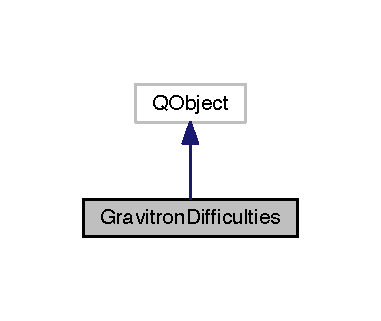
\includegraphics[width=183pt]{class_gravitron_difficulties__inherit__graph}
\end{center}
\end{figure}


Collaboration diagram for Gravitron\+Difficulties\+:\nopagebreak
\begin{figure}[H]
\begin{center}
\leavevmode
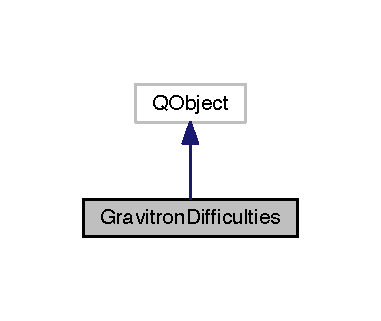
\includegraphics[width=183pt]{class_gravitron_difficulties__coll__graph}
\end{center}
\end{figure}
\subsection*{Public Types}
\begin{DoxyCompactItemize}
\item 
enum \hyperlink{class_gravitron_difficulties_a750335ce46507e59ed2920c727961a7c}{Enum\+Difficulies} \{ \hyperlink{class_gravitron_difficulties_a750335ce46507e59ed2920c727961a7ca5d10ab2ad81fb31656419749c3fe8d8e}{E\+A\+S\+Y}, 
\hyperlink{class_gravitron_difficulties_a750335ce46507e59ed2920c727961a7ca042903b48121b0977d01e2434590000b}{M\+I\+D\+D\+L\+E}, 
\hyperlink{class_gravitron_difficulties_a750335ce46507e59ed2920c727961a7ca6749d46a3ece9db0bd0f2b0888495617}{H\+A\+R\+D}
 \}
\end{DoxyCompactItemize}


\subsection{Member Enumeration Documentation}
\hypertarget{class_gravitron_difficulties_a750335ce46507e59ed2920c727961a7c}{\index{Gravitron\+Difficulties@{Gravitron\+Difficulties}!Enum\+Difficulies@{Enum\+Difficulies}}
\index{Enum\+Difficulies@{Enum\+Difficulies}!Gravitron\+Difficulties@{Gravitron\+Difficulties}}
\subsubsection[{Enum\+Difficulies}]{\setlength{\rightskip}{0pt plus 5cm}enum {\bf Gravitron\+Difficulties\+::\+Enum\+Difficulies}}}\label{class_gravitron_difficulties_a750335ce46507e59ed2920c727961a7c}
\begin{Desc}
\item[Enumerator]\par
\begin{description}
\index{E\+A\+S\+Y@{E\+A\+S\+Y}!Gravitron\+Difficulties@{Gravitron\+Difficulties}}\index{Gravitron\+Difficulties@{Gravitron\+Difficulties}!E\+A\+S\+Y@{E\+A\+S\+Y}}\item[{\em 
\hypertarget{class_gravitron_difficulties_a750335ce46507e59ed2920c727961a7ca5d10ab2ad81fb31656419749c3fe8d8e}{E\+A\+S\+Y}\label{class_gravitron_difficulties_a750335ce46507e59ed2920c727961a7ca5d10ab2ad81fb31656419749c3fe8d8e}
}]\index{M\+I\+D\+D\+L\+E@{M\+I\+D\+D\+L\+E}!Gravitron\+Difficulties@{Gravitron\+Difficulties}}\index{Gravitron\+Difficulties@{Gravitron\+Difficulties}!M\+I\+D\+D\+L\+E@{M\+I\+D\+D\+L\+E}}\item[{\em 
\hypertarget{class_gravitron_difficulties_a750335ce46507e59ed2920c727961a7ca042903b48121b0977d01e2434590000b}{M\+I\+D\+D\+L\+E}\label{class_gravitron_difficulties_a750335ce46507e59ed2920c727961a7ca042903b48121b0977d01e2434590000b}
}]\index{H\+A\+R\+D@{H\+A\+R\+D}!Gravitron\+Difficulties@{Gravitron\+Difficulties}}\index{Gravitron\+Difficulties@{Gravitron\+Difficulties}!H\+A\+R\+D@{H\+A\+R\+D}}\item[{\em 
\hypertarget{class_gravitron_difficulties_a750335ce46507e59ed2920c727961a7ca6749d46a3ece9db0bd0f2b0888495617}{H\+A\+R\+D}\label{class_gravitron_difficulties_a750335ce46507e59ed2920c727961a7ca6749d46a3ece9db0bd0f2b0888495617}
}]\end{description}
\end{Desc}


The documentation for this class was generated from the following file\+:\begin{DoxyCompactItemize}
\item 
src/headers/\hyperlink{_gravitron_difficulties_8h}{Gravitron\+Difficulties.\+h}\end{DoxyCompactItemize}

\hypertarget{class_gravitron_settings}{\section{Gravitron\+Settings Class Reference}
\label{class_gravitron_settings}\index{Gravitron\+Settings@{Gravitron\+Settings}}
}


{\ttfamily \#include $<$Gravitron\+Settings.\+h$>$}



Inheritance diagram for Gravitron\+Settings\+:\nopagebreak
\begin{figure}[H]
\begin{center}
\leavevmode
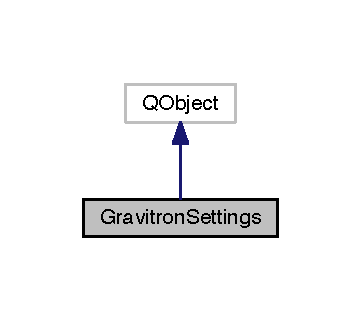
\includegraphics[width=173pt]{class_gravitron_settings__inherit__graph}
\end{center}
\end{figure}


Collaboration diagram for Gravitron\+Settings\+:\nopagebreak
\begin{figure}[H]
\begin{center}
\leavevmode
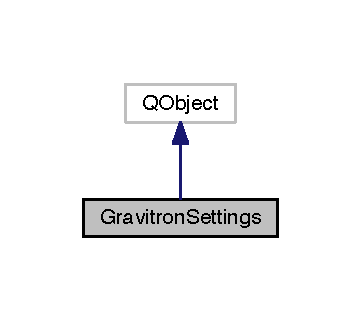
\includegraphics[width=173pt]{class_gravitron_settings__coll__graph}
\end{center}
\end{figure}
\subsection*{Signals}
\begin{DoxyCompactItemize}
\item 
void \hyperlink{class_gravitron_settings_a997bf69a2e778b7bbd6beefae8ee8578}{difficulty\+Changed} (const int \&source)
\item 
void \hyperlink{class_gravitron_settings_ac97163add79f61d978415fdc55beef2d}{full\+Screen\+Changed} (const bool \&source)
\item 
void \hyperlink{class_gravitron_settings_a481cf99de16e994c63c3dfeff94123fe}{music\+Sound\+Volume\+Changed} (const int \&source)
\item 
void \hyperlink{class_gravitron_settings_a101f009286632eb4f3c0f10274308200}{play\+Music\+Changed} (const bool \&source)
\item 
void \hyperlink{class_gravitron_settings_a87e9774036049c9593dc5779a94ba6a4}{play\+Sounds\+Changed} (const bool \&source)
\item 
void \hyperlink{class_gravitron_settings_ab12347fa7a95663bf557d703d82d980f}{player\+Name\+Changed} (const Q\+String \&source)
\item 
void \hyperlink{class_gravitron_settings_aaeb6b5aa718d90074b71a8da747d535e}{playing\+Field\+Size\+Changed} (const int \&source)
\item 
void \hyperlink{class_gravitron_settings_a28457660e35d741279ada2a98f6ebd4d}{bots\+Count\+Changed} (const int \&source)
\item 
void \hyperlink{class_gravitron_settings_ac4b5df1b082308bd710280080f1caee6}{planet\+Count\+Changed} (const int \&source)
\item 
void \hyperlink{class_gravitron_settings_a443c7369cc5836f6ea4f98de603ad9e5}{astroid\+Count\+Changed} (const int \&source)
\item 
void \hyperlink{class_gravitron_settings_a79ceaa5ff5b0e30a6b144a92a513c470}{frag\+Changed} (const int \&source)
\item 
void \hyperlink{class_gravitron_settings_aab8e8dddbae563d26becd6279d727788}{respaw\+Time\+Changed} (const int \&source)
\item 
void \hyperlink{class_gravitron_settings_a469a7cb1c07c6f9a9fb905ed535c4244}{languare\+Changed} (const Q\+String \&source)
\item 
void \hyperlink{class_gravitron_settings_a2a953f97e01ec9de394bd8b2d23c3bbc}{error} (const Q\+String \&msg)
\end{DoxyCompactItemize}
\subsection*{Public Member Functions}
\begin{DoxyCompactItemize}
\item 
\hyperlink{class_gravitron_settings_a6cb102251aabe6808b03882e891b7bbf}{Gravitron\+Settings} (Q\+Object $\ast$parent=0)
\item 
Q\+\_\+\+I\+N\+V\+O\+K\+A\+B\+L\+E int \hyperlink{class_gravitron_settings_afe99529e5133887abc2ec6cdf05ae319}{difficulty} () const 
\item 
Q\+\_\+\+I\+N\+V\+O\+K\+A\+B\+L\+E void \hyperlink{class_gravitron_settings_ae8240cfb314457bd03e7053c0fe69aa3}{set\+Difficulty} (const int \&source)
\item 
Q\+\_\+\+I\+N\+V\+O\+K\+A\+B\+L\+E int \hyperlink{class_gravitron_settings_afa85ead0e4713679fa5b7e33aa7a5eee}{full\+Screen} () const 
\item 
Q\+\_\+\+I\+N\+V\+O\+K\+A\+B\+L\+E void \hyperlink{class_gravitron_settings_a63094c938fb60cc79ca096dd2444745a}{set\+Full\+Screen} (const bool \&source)
\item 
Q\+\_\+\+I\+N\+V\+O\+K\+A\+B\+L\+E int \hyperlink{class_gravitron_settings_ace2f3ca4ca6680832e14b546097a7f59}{music\+Sound\+Volume} () const 
\item 
Q\+\_\+\+I\+N\+V\+O\+K\+A\+B\+L\+E void \hyperlink{class_gravitron_settings_a19127cb8ad9035391cef6607ebfcfbd8}{set\+Music\+Sound\+Volume} (const int \&source)
\item 
Q\+\_\+\+I\+N\+V\+O\+K\+A\+B\+L\+E bool \hyperlink{class_gravitron_settings_a609265806b2879e7210f2d3a12b88f45}{play\+Music} () const 
\item 
Q\+\_\+\+I\+N\+V\+O\+K\+A\+B\+L\+E void \hyperlink{class_gravitron_settings_afcaa509baf03618793cc7fcfb5ef2030}{set\+Play\+Music} (const bool \&source)
\item 
Q\+\_\+\+I\+N\+V\+O\+K\+A\+B\+L\+E bool \hyperlink{class_gravitron_settings_aa412b289968c89d9e6e2ebd8932260bf}{play\+Sounds} () const 
\item 
Q\+\_\+\+I\+N\+V\+O\+K\+A\+B\+L\+E void \hyperlink{class_gravitron_settings_a658374f96e4bb64f91e770a6df87cc69}{set\+Play\+Sounds} (const bool \&source)
\item 
Q\+\_\+\+I\+N\+V\+O\+K\+A\+B\+L\+E Q\+String \hyperlink{class_gravitron_settings_a8e707f83dc20e85cd0632a858787cf7d}{player\+Name} () const 
\item 
Q\+\_\+\+I\+N\+V\+O\+K\+A\+B\+L\+E void \hyperlink{class_gravitron_settings_ac6dc8d0025905248e80217198513a044}{set\+Player\+Name} (const Q\+String \&source)
\item 
Q\+\_\+\+I\+N\+V\+O\+K\+A\+B\+L\+E int \hyperlink{class_gravitron_settings_ac42974dae44eec47f9188ead3b950251}{playing\+Field\+Size} () const 
\item 
Q\+\_\+\+I\+N\+V\+O\+K\+A\+B\+L\+E void \hyperlink{class_gravitron_settings_aaceaf8068d09b9e22d8085c6ca3db2d8}{set\+Playing\+Field\+Size} (const int \&source)
\item 
Q\+\_\+\+I\+N\+V\+O\+K\+A\+B\+L\+E int \hyperlink{class_gravitron_settings_a0111fc2b9a795979bc59026ae6bf9193}{bots\+Count} () const 
\item 
Q\+\_\+\+I\+N\+V\+O\+K\+A\+B\+L\+E void \hyperlink{class_gravitron_settings_ac2ec7898b33cbd349497c59f69ee7c1d}{set\+Bots\+Count} (const int \&source)
\item 
Q\+\_\+\+I\+N\+V\+O\+K\+A\+B\+L\+E int \hyperlink{class_gravitron_settings_aeb6526e7912b3aa7a402de993bb81981}{planet\+Count} () const 
\item 
Q\+\_\+\+I\+N\+V\+O\+K\+A\+B\+L\+E void \hyperlink{class_gravitron_settings_a1bb8463107c3236fd2610c657b4ffe59}{set\+Planet\+Count} (const int \&source)
\item 
Q\+\_\+\+I\+N\+V\+O\+K\+A\+B\+L\+E int \hyperlink{class_gravitron_settings_a4e31985e206c8e62adeddcf90b86d3b4}{astroid\+Count} () const 
\item 
Q\+\_\+\+I\+N\+V\+O\+K\+A\+B\+L\+E void \hyperlink{class_gravitron_settings_a0f48fe8d1d9fc850ac5272fffdc66c45}{set\+Astroid\+Count} (const int \&source)
\item 
Q\+\_\+\+I\+N\+V\+O\+K\+A\+B\+L\+E int \hyperlink{class_gravitron_settings_aaa360d47801ac1c5a32085d899ec09fd}{frag} () const 
\item 
Q\+\_\+\+I\+N\+V\+O\+K\+A\+B\+L\+E void \hyperlink{class_gravitron_settings_a68c312fe2c90b7aa39951751ffdc0be6}{set\+Frag} (const int \&source)
\item 
Q\+\_\+\+I\+N\+V\+O\+K\+A\+B\+L\+E int \hyperlink{class_gravitron_settings_ac80d618a1e99de9bc697827e3b5c0749}{respaw\+Time} () const 
\item 
Q\+\_\+\+I\+N\+V\+O\+K\+A\+B\+L\+E void \hyperlink{class_gravitron_settings_a4263bace900a630e49d498114102b181}{set\+Respaw\+Time} (const int \&source)
\item 
Q\+\_\+\+I\+N\+V\+O\+K\+A\+B\+L\+E Q\+String \hyperlink{class_gravitron_settings_a334450cf29acbebb01262a5d945f7e24}{languare} () const 
\item 
Q\+\_\+\+I\+N\+V\+O\+K\+A\+B\+L\+E void \hyperlink{class_gravitron_settings_a1c457b47d88c01a5c3541f3c861fcda6}{set\+Languare} (const Q\+String \&source)
\item 
Q\+\_\+\+I\+N\+V\+O\+K\+A\+B\+L\+E bool \hyperlink{class_gravitron_settings_aab42e5f608b9e46d077a1418cd9d709d}{network} () const 
\item 
Q\+\_\+\+I\+N\+V\+O\+K\+A\+B\+L\+E void \hyperlink{class_gravitron_settings_a27abb8747f90faa675cf875962a4cb17}{set\+Network} (const bool \&source)
\item 
void \hyperlink{class_gravitron_settings_a058ae43b2b186753956a8f9e4c54234b}{save} ()
\item 
void \hyperlink{class_gravitron_settings_ad7226f0a103f0aea9786904a537ef1c1}{load} ()
\end{DoxyCompactItemize}
\subsection*{Friends}
\begin{DoxyCompactItemize}
\item 
Q\+Data\+Stream \& \hyperlink{class_gravitron_settings_a24a8274b8fa276e0da0ebf0e6fc3d176}{operator$<$$<$} (Q\+Data\+Stream \&stream, const \hyperlink{class_gravitron_settings}{Gravitron\+Settings} \&settings)
\item 
Q\+Data\+Stream \& \hyperlink{class_gravitron_settings_a652a2b630485f03a4a527ef3ef7a3367}{operator$>$$>$} (Q\+Data\+Stream \&stream, \hyperlink{class_gravitron_settings}{Gravitron\+Settings} \&settings)
\end{DoxyCompactItemize}


\subsection{Constructor \& Destructor Documentation}
\hypertarget{class_gravitron_settings_a6cb102251aabe6808b03882e891b7bbf}{\index{Gravitron\+Settings@{Gravitron\+Settings}!Gravitron\+Settings@{Gravitron\+Settings}}
\index{Gravitron\+Settings@{Gravitron\+Settings}!Gravitron\+Settings@{Gravitron\+Settings}}
\subsubsection[{Gravitron\+Settings}]{\setlength{\rightskip}{0pt plus 5cm}Gravitron\+Settings\+::\+Gravitron\+Settings (
\begin{DoxyParamCaption}
\item[{Q\+Object $\ast$}]{parent = {\ttfamily 0}}
\end{DoxyParamCaption}
)\hspace{0.3cm}{\ttfamily [explicit]}}}\label{class_gravitron_settings_a6cb102251aabe6808b03882e891b7bbf}


Here is the call graph for this function\+:\nopagebreak
\begin{figure}[H]
\begin{center}
\leavevmode
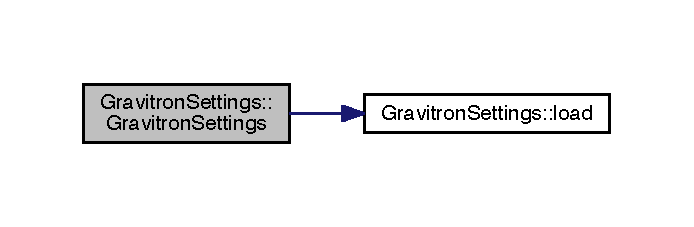
\includegraphics[width=333pt]{class_gravitron_settings_a6cb102251aabe6808b03882e891b7bbf_cgraph}
\end{center}
\end{figure}




\subsection{Member Function Documentation}
\hypertarget{class_gravitron_settings_a4e31985e206c8e62adeddcf90b86d3b4}{\index{Gravitron\+Settings@{Gravitron\+Settings}!astroid\+Count@{astroid\+Count}}
\index{astroid\+Count@{astroid\+Count}!Gravitron\+Settings@{Gravitron\+Settings}}
\subsubsection[{astroid\+Count}]{\setlength{\rightskip}{0pt plus 5cm}Q\+\_\+\+I\+N\+V\+O\+K\+A\+B\+L\+E int Gravitron\+Settings\+::astroid\+Count (
\begin{DoxyParamCaption}
{}
\end{DoxyParamCaption}
) const}}\label{class_gravitron_settings_a4e31985e206c8e62adeddcf90b86d3b4}
\hypertarget{class_gravitron_settings_a443c7369cc5836f6ea4f98de603ad9e5}{\index{Gravitron\+Settings@{Gravitron\+Settings}!astroid\+Count\+Changed@{astroid\+Count\+Changed}}
\index{astroid\+Count\+Changed@{astroid\+Count\+Changed}!Gravitron\+Settings@{Gravitron\+Settings}}
\subsubsection[{astroid\+Count\+Changed}]{\setlength{\rightskip}{0pt plus 5cm}void Gravitron\+Settings\+::astroid\+Count\+Changed (
\begin{DoxyParamCaption}
\item[{const int \&}]{source}
\end{DoxyParamCaption}
)\hspace{0.3cm}{\ttfamily [signal]}}}\label{class_gravitron_settings_a443c7369cc5836f6ea4f98de603ad9e5}
\hypertarget{class_gravitron_settings_a0111fc2b9a795979bc59026ae6bf9193}{\index{Gravitron\+Settings@{Gravitron\+Settings}!bots\+Count@{bots\+Count}}
\index{bots\+Count@{bots\+Count}!Gravitron\+Settings@{Gravitron\+Settings}}
\subsubsection[{bots\+Count}]{\setlength{\rightskip}{0pt plus 5cm}Q\+\_\+\+I\+N\+V\+O\+K\+A\+B\+L\+E int Gravitron\+Settings\+::bots\+Count (
\begin{DoxyParamCaption}
{}
\end{DoxyParamCaption}
) const}}\label{class_gravitron_settings_a0111fc2b9a795979bc59026ae6bf9193}
\hypertarget{class_gravitron_settings_a28457660e35d741279ada2a98f6ebd4d}{\index{Gravitron\+Settings@{Gravitron\+Settings}!bots\+Count\+Changed@{bots\+Count\+Changed}}
\index{bots\+Count\+Changed@{bots\+Count\+Changed}!Gravitron\+Settings@{Gravitron\+Settings}}
\subsubsection[{bots\+Count\+Changed}]{\setlength{\rightskip}{0pt plus 5cm}void Gravitron\+Settings\+::bots\+Count\+Changed (
\begin{DoxyParamCaption}
\item[{const int \&}]{source}
\end{DoxyParamCaption}
)\hspace{0.3cm}{\ttfamily [signal]}}}\label{class_gravitron_settings_a28457660e35d741279ada2a98f6ebd4d}
\hypertarget{class_gravitron_settings_afe99529e5133887abc2ec6cdf05ae319}{\index{Gravitron\+Settings@{Gravitron\+Settings}!difficulty@{difficulty}}
\index{difficulty@{difficulty}!Gravitron\+Settings@{Gravitron\+Settings}}
\subsubsection[{difficulty}]{\setlength{\rightskip}{0pt plus 5cm}Q\+\_\+\+I\+N\+V\+O\+K\+A\+B\+L\+E int Gravitron\+Settings\+::difficulty (
\begin{DoxyParamCaption}
{}
\end{DoxyParamCaption}
) const}}\label{class_gravitron_settings_afe99529e5133887abc2ec6cdf05ae319}
\hypertarget{class_gravitron_settings_a997bf69a2e778b7bbd6beefae8ee8578}{\index{Gravitron\+Settings@{Gravitron\+Settings}!difficulty\+Changed@{difficulty\+Changed}}
\index{difficulty\+Changed@{difficulty\+Changed}!Gravitron\+Settings@{Gravitron\+Settings}}
\subsubsection[{difficulty\+Changed}]{\setlength{\rightskip}{0pt plus 5cm}void Gravitron\+Settings\+::difficulty\+Changed (
\begin{DoxyParamCaption}
\item[{const int \&}]{source}
\end{DoxyParamCaption}
)\hspace{0.3cm}{\ttfamily [signal]}}}\label{class_gravitron_settings_a997bf69a2e778b7bbd6beefae8ee8578}
\hypertarget{class_gravitron_settings_a2a953f97e01ec9de394bd8b2d23c3bbc}{\index{Gravitron\+Settings@{Gravitron\+Settings}!error@{error}}
\index{error@{error}!Gravitron\+Settings@{Gravitron\+Settings}}
\subsubsection[{error}]{\setlength{\rightskip}{0pt plus 5cm}void Gravitron\+Settings\+::error (
\begin{DoxyParamCaption}
\item[{const Q\+String \&}]{msg}
\end{DoxyParamCaption}
)\hspace{0.3cm}{\ttfamily [signal]}}}\label{class_gravitron_settings_a2a953f97e01ec9de394bd8b2d23c3bbc}
\hypertarget{class_gravitron_settings_aaa360d47801ac1c5a32085d899ec09fd}{\index{Gravitron\+Settings@{Gravitron\+Settings}!frag@{frag}}
\index{frag@{frag}!Gravitron\+Settings@{Gravitron\+Settings}}
\subsubsection[{frag}]{\setlength{\rightskip}{0pt plus 5cm}Q\+\_\+\+I\+N\+V\+O\+K\+A\+B\+L\+E int Gravitron\+Settings\+::frag (
\begin{DoxyParamCaption}
{}
\end{DoxyParamCaption}
) const}}\label{class_gravitron_settings_aaa360d47801ac1c5a32085d899ec09fd}
\hypertarget{class_gravitron_settings_a79ceaa5ff5b0e30a6b144a92a513c470}{\index{Gravitron\+Settings@{Gravitron\+Settings}!frag\+Changed@{frag\+Changed}}
\index{frag\+Changed@{frag\+Changed}!Gravitron\+Settings@{Gravitron\+Settings}}
\subsubsection[{frag\+Changed}]{\setlength{\rightskip}{0pt plus 5cm}void Gravitron\+Settings\+::frag\+Changed (
\begin{DoxyParamCaption}
\item[{const int \&}]{source}
\end{DoxyParamCaption}
)\hspace{0.3cm}{\ttfamily [signal]}}}\label{class_gravitron_settings_a79ceaa5ff5b0e30a6b144a92a513c470}
\hypertarget{class_gravitron_settings_afa85ead0e4713679fa5b7e33aa7a5eee}{\index{Gravitron\+Settings@{Gravitron\+Settings}!full\+Screen@{full\+Screen}}
\index{full\+Screen@{full\+Screen}!Gravitron\+Settings@{Gravitron\+Settings}}
\subsubsection[{full\+Screen}]{\setlength{\rightskip}{0pt plus 5cm}Q\+\_\+\+I\+N\+V\+O\+K\+A\+B\+L\+E int Gravitron\+Settings\+::full\+Screen (
\begin{DoxyParamCaption}
{}
\end{DoxyParamCaption}
) const}}\label{class_gravitron_settings_afa85ead0e4713679fa5b7e33aa7a5eee}
\hypertarget{class_gravitron_settings_ac97163add79f61d978415fdc55beef2d}{\index{Gravitron\+Settings@{Gravitron\+Settings}!full\+Screen\+Changed@{full\+Screen\+Changed}}
\index{full\+Screen\+Changed@{full\+Screen\+Changed}!Gravitron\+Settings@{Gravitron\+Settings}}
\subsubsection[{full\+Screen\+Changed}]{\setlength{\rightskip}{0pt plus 5cm}void Gravitron\+Settings\+::full\+Screen\+Changed (
\begin{DoxyParamCaption}
\item[{const bool \&}]{source}
\end{DoxyParamCaption}
)\hspace{0.3cm}{\ttfamily [signal]}}}\label{class_gravitron_settings_ac97163add79f61d978415fdc55beef2d}
\hypertarget{class_gravitron_settings_a334450cf29acbebb01262a5d945f7e24}{\index{Gravitron\+Settings@{Gravitron\+Settings}!languare@{languare}}
\index{languare@{languare}!Gravitron\+Settings@{Gravitron\+Settings}}
\subsubsection[{languare}]{\setlength{\rightskip}{0pt plus 5cm}Q\+\_\+\+I\+N\+V\+O\+K\+A\+B\+L\+E Q\+String Gravitron\+Settings\+::languare (
\begin{DoxyParamCaption}
{}
\end{DoxyParamCaption}
) const}}\label{class_gravitron_settings_a334450cf29acbebb01262a5d945f7e24}
\hypertarget{class_gravitron_settings_a469a7cb1c07c6f9a9fb905ed535c4244}{\index{Gravitron\+Settings@{Gravitron\+Settings}!languare\+Changed@{languare\+Changed}}
\index{languare\+Changed@{languare\+Changed}!Gravitron\+Settings@{Gravitron\+Settings}}
\subsubsection[{languare\+Changed}]{\setlength{\rightskip}{0pt plus 5cm}void Gravitron\+Settings\+::languare\+Changed (
\begin{DoxyParamCaption}
\item[{const Q\+String \&}]{source}
\end{DoxyParamCaption}
)\hspace{0.3cm}{\ttfamily [signal]}}}\label{class_gravitron_settings_a469a7cb1c07c6f9a9fb905ed535c4244}
\hypertarget{class_gravitron_settings_ad7226f0a103f0aea9786904a537ef1c1}{\index{Gravitron\+Settings@{Gravitron\+Settings}!load@{load}}
\index{load@{load}!Gravitron\+Settings@{Gravitron\+Settings}}
\subsubsection[{load}]{\setlength{\rightskip}{0pt plus 5cm}void Gravitron\+Settings\+::load (
\begin{DoxyParamCaption}
{}
\end{DoxyParamCaption}
)}}\label{class_gravitron_settings_ad7226f0a103f0aea9786904a537ef1c1}
\hypertarget{class_gravitron_settings_ace2f3ca4ca6680832e14b546097a7f59}{\index{Gravitron\+Settings@{Gravitron\+Settings}!music\+Sound\+Volume@{music\+Sound\+Volume}}
\index{music\+Sound\+Volume@{music\+Sound\+Volume}!Gravitron\+Settings@{Gravitron\+Settings}}
\subsubsection[{music\+Sound\+Volume}]{\setlength{\rightskip}{0pt plus 5cm}Q\+\_\+\+I\+N\+V\+O\+K\+A\+B\+L\+E int Gravitron\+Settings\+::music\+Sound\+Volume (
\begin{DoxyParamCaption}
{}
\end{DoxyParamCaption}
) const}}\label{class_gravitron_settings_ace2f3ca4ca6680832e14b546097a7f59}
\hypertarget{class_gravitron_settings_a481cf99de16e994c63c3dfeff94123fe}{\index{Gravitron\+Settings@{Gravitron\+Settings}!music\+Sound\+Volume\+Changed@{music\+Sound\+Volume\+Changed}}
\index{music\+Sound\+Volume\+Changed@{music\+Sound\+Volume\+Changed}!Gravitron\+Settings@{Gravitron\+Settings}}
\subsubsection[{music\+Sound\+Volume\+Changed}]{\setlength{\rightskip}{0pt plus 5cm}void Gravitron\+Settings\+::music\+Sound\+Volume\+Changed (
\begin{DoxyParamCaption}
\item[{const int \&}]{source}
\end{DoxyParamCaption}
)\hspace{0.3cm}{\ttfamily [signal]}}}\label{class_gravitron_settings_a481cf99de16e994c63c3dfeff94123fe}
\hypertarget{class_gravitron_settings_aab42e5f608b9e46d077a1418cd9d709d}{\index{Gravitron\+Settings@{Gravitron\+Settings}!network@{network}}
\index{network@{network}!Gravitron\+Settings@{Gravitron\+Settings}}
\subsubsection[{network}]{\setlength{\rightskip}{0pt plus 5cm}Q\+\_\+\+I\+N\+V\+O\+K\+A\+B\+L\+E bool Gravitron\+Settings\+::network (
\begin{DoxyParamCaption}
{}
\end{DoxyParamCaption}
) const}}\label{class_gravitron_settings_aab42e5f608b9e46d077a1418cd9d709d}
\hypertarget{class_gravitron_settings_aeb6526e7912b3aa7a402de993bb81981}{\index{Gravitron\+Settings@{Gravitron\+Settings}!planet\+Count@{planet\+Count}}
\index{planet\+Count@{planet\+Count}!Gravitron\+Settings@{Gravitron\+Settings}}
\subsubsection[{planet\+Count}]{\setlength{\rightskip}{0pt plus 5cm}Q\+\_\+\+I\+N\+V\+O\+K\+A\+B\+L\+E int Gravitron\+Settings\+::planet\+Count (
\begin{DoxyParamCaption}
{}
\end{DoxyParamCaption}
) const}}\label{class_gravitron_settings_aeb6526e7912b3aa7a402de993bb81981}
\hypertarget{class_gravitron_settings_ac4b5df1b082308bd710280080f1caee6}{\index{Gravitron\+Settings@{Gravitron\+Settings}!planet\+Count\+Changed@{planet\+Count\+Changed}}
\index{planet\+Count\+Changed@{planet\+Count\+Changed}!Gravitron\+Settings@{Gravitron\+Settings}}
\subsubsection[{planet\+Count\+Changed}]{\setlength{\rightskip}{0pt plus 5cm}void Gravitron\+Settings\+::planet\+Count\+Changed (
\begin{DoxyParamCaption}
\item[{const int \&}]{source}
\end{DoxyParamCaption}
)\hspace{0.3cm}{\ttfamily [signal]}}}\label{class_gravitron_settings_ac4b5df1b082308bd710280080f1caee6}
\hypertarget{class_gravitron_settings_a8e707f83dc20e85cd0632a858787cf7d}{\index{Gravitron\+Settings@{Gravitron\+Settings}!player\+Name@{player\+Name}}
\index{player\+Name@{player\+Name}!Gravitron\+Settings@{Gravitron\+Settings}}
\subsubsection[{player\+Name}]{\setlength{\rightskip}{0pt plus 5cm}Q\+\_\+\+I\+N\+V\+O\+K\+A\+B\+L\+E Q\+String Gravitron\+Settings\+::player\+Name (
\begin{DoxyParamCaption}
{}
\end{DoxyParamCaption}
) const}}\label{class_gravitron_settings_a8e707f83dc20e85cd0632a858787cf7d}
\hypertarget{class_gravitron_settings_ab12347fa7a95663bf557d703d82d980f}{\index{Gravitron\+Settings@{Gravitron\+Settings}!player\+Name\+Changed@{player\+Name\+Changed}}
\index{player\+Name\+Changed@{player\+Name\+Changed}!Gravitron\+Settings@{Gravitron\+Settings}}
\subsubsection[{player\+Name\+Changed}]{\setlength{\rightskip}{0pt plus 5cm}void Gravitron\+Settings\+::player\+Name\+Changed (
\begin{DoxyParamCaption}
\item[{const Q\+String \&}]{source}
\end{DoxyParamCaption}
)\hspace{0.3cm}{\ttfamily [signal]}}}\label{class_gravitron_settings_ab12347fa7a95663bf557d703d82d980f}
\hypertarget{class_gravitron_settings_ac42974dae44eec47f9188ead3b950251}{\index{Gravitron\+Settings@{Gravitron\+Settings}!playing\+Field\+Size@{playing\+Field\+Size}}
\index{playing\+Field\+Size@{playing\+Field\+Size}!Gravitron\+Settings@{Gravitron\+Settings}}
\subsubsection[{playing\+Field\+Size}]{\setlength{\rightskip}{0pt plus 5cm}Q\+\_\+\+I\+N\+V\+O\+K\+A\+B\+L\+E int Gravitron\+Settings\+::playing\+Field\+Size (
\begin{DoxyParamCaption}
{}
\end{DoxyParamCaption}
) const}}\label{class_gravitron_settings_ac42974dae44eec47f9188ead3b950251}
\hypertarget{class_gravitron_settings_aaeb6b5aa718d90074b71a8da747d535e}{\index{Gravitron\+Settings@{Gravitron\+Settings}!playing\+Field\+Size\+Changed@{playing\+Field\+Size\+Changed}}
\index{playing\+Field\+Size\+Changed@{playing\+Field\+Size\+Changed}!Gravitron\+Settings@{Gravitron\+Settings}}
\subsubsection[{playing\+Field\+Size\+Changed}]{\setlength{\rightskip}{0pt plus 5cm}void Gravitron\+Settings\+::playing\+Field\+Size\+Changed (
\begin{DoxyParamCaption}
\item[{const int \&}]{source}
\end{DoxyParamCaption}
)\hspace{0.3cm}{\ttfamily [signal]}}}\label{class_gravitron_settings_aaeb6b5aa718d90074b71a8da747d535e}
\hypertarget{class_gravitron_settings_a609265806b2879e7210f2d3a12b88f45}{\index{Gravitron\+Settings@{Gravitron\+Settings}!play\+Music@{play\+Music}}
\index{play\+Music@{play\+Music}!Gravitron\+Settings@{Gravitron\+Settings}}
\subsubsection[{play\+Music}]{\setlength{\rightskip}{0pt plus 5cm}Q\+\_\+\+I\+N\+V\+O\+K\+A\+B\+L\+E bool Gravitron\+Settings\+::play\+Music (
\begin{DoxyParamCaption}
{}
\end{DoxyParamCaption}
) const}}\label{class_gravitron_settings_a609265806b2879e7210f2d3a12b88f45}
\hypertarget{class_gravitron_settings_a101f009286632eb4f3c0f10274308200}{\index{Gravitron\+Settings@{Gravitron\+Settings}!play\+Music\+Changed@{play\+Music\+Changed}}
\index{play\+Music\+Changed@{play\+Music\+Changed}!Gravitron\+Settings@{Gravitron\+Settings}}
\subsubsection[{play\+Music\+Changed}]{\setlength{\rightskip}{0pt plus 5cm}void Gravitron\+Settings\+::play\+Music\+Changed (
\begin{DoxyParamCaption}
\item[{const bool \&}]{source}
\end{DoxyParamCaption}
)\hspace{0.3cm}{\ttfamily [signal]}}}\label{class_gravitron_settings_a101f009286632eb4f3c0f10274308200}
\hypertarget{class_gravitron_settings_aa412b289968c89d9e6e2ebd8932260bf}{\index{Gravitron\+Settings@{Gravitron\+Settings}!play\+Sounds@{play\+Sounds}}
\index{play\+Sounds@{play\+Sounds}!Gravitron\+Settings@{Gravitron\+Settings}}
\subsubsection[{play\+Sounds}]{\setlength{\rightskip}{0pt plus 5cm}Q\+\_\+\+I\+N\+V\+O\+K\+A\+B\+L\+E bool Gravitron\+Settings\+::play\+Sounds (
\begin{DoxyParamCaption}
{}
\end{DoxyParamCaption}
) const}}\label{class_gravitron_settings_aa412b289968c89d9e6e2ebd8932260bf}
\hypertarget{class_gravitron_settings_a87e9774036049c9593dc5779a94ba6a4}{\index{Gravitron\+Settings@{Gravitron\+Settings}!play\+Sounds\+Changed@{play\+Sounds\+Changed}}
\index{play\+Sounds\+Changed@{play\+Sounds\+Changed}!Gravitron\+Settings@{Gravitron\+Settings}}
\subsubsection[{play\+Sounds\+Changed}]{\setlength{\rightskip}{0pt plus 5cm}void Gravitron\+Settings\+::play\+Sounds\+Changed (
\begin{DoxyParamCaption}
\item[{const bool \&}]{source}
\end{DoxyParamCaption}
)\hspace{0.3cm}{\ttfamily [signal]}}}\label{class_gravitron_settings_a87e9774036049c9593dc5779a94ba6a4}
\hypertarget{class_gravitron_settings_ac80d618a1e99de9bc697827e3b5c0749}{\index{Gravitron\+Settings@{Gravitron\+Settings}!respaw\+Time@{respaw\+Time}}
\index{respaw\+Time@{respaw\+Time}!Gravitron\+Settings@{Gravitron\+Settings}}
\subsubsection[{respaw\+Time}]{\setlength{\rightskip}{0pt plus 5cm}Q\+\_\+\+I\+N\+V\+O\+K\+A\+B\+L\+E int Gravitron\+Settings\+::respaw\+Time (
\begin{DoxyParamCaption}
{}
\end{DoxyParamCaption}
) const}}\label{class_gravitron_settings_ac80d618a1e99de9bc697827e3b5c0749}
\hypertarget{class_gravitron_settings_aab8e8dddbae563d26becd6279d727788}{\index{Gravitron\+Settings@{Gravitron\+Settings}!respaw\+Time\+Changed@{respaw\+Time\+Changed}}
\index{respaw\+Time\+Changed@{respaw\+Time\+Changed}!Gravitron\+Settings@{Gravitron\+Settings}}
\subsubsection[{respaw\+Time\+Changed}]{\setlength{\rightskip}{0pt plus 5cm}void Gravitron\+Settings\+::respaw\+Time\+Changed (
\begin{DoxyParamCaption}
\item[{const int \&}]{source}
\end{DoxyParamCaption}
)\hspace{0.3cm}{\ttfamily [signal]}}}\label{class_gravitron_settings_aab8e8dddbae563d26becd6279d727788}
\hypertarget{class_gravitron_settings_a058ae43b2b186753956a8f9e4c54234b}{\index{Gravitron\+Settings@{Gravitron\+Settings}!save@{save}}
\index{save@{save}!Gravitron\+Settings@{Gravitron\+Settings}}
\subsubsection[{save}]{\setlength{\rightskip}{0pt plus 5cm}void Gravitron\+Settings\+::save (
\begin{DoxyParamCaption}
{}
\end{DoxyParamCaption}
)}}\label{class_gravitron_settings_a058ae43b2b186753956a8f9e4c54234b}
\hypertarget{class_gravitron_settings_a0f48fe8d1d9fc850ac5272fffdc66c45}{\index{Gravitron\+Settings@{Gravitron\+Settings}!set\+Astroid\+Count@{set\+Astroid\+Count}}
\index{set\+Astroid\+Count@{set\+Astroid\+Count}!Gravitron\+Settings@{Gravitron\+Settings}}
\subsubsection[{set\+Astroid\+Count}]{\setlength{\rightskip}{0pt plus 5cm}void Gravitron\+Settings\+::set\+Astroid\+Count (
\begin{DoxyParamCaption}
\item[{const int \&}]{source}
\end{DoxyParamCaption}
)}}\label{class_gravitron_settings_a0f48fe8d1d9fc850ac5272fffdc66c45}


Here is the call graph for this function\+:\nopagebreak
\begin{figure}[H]
\begin{center}
\leavevmode
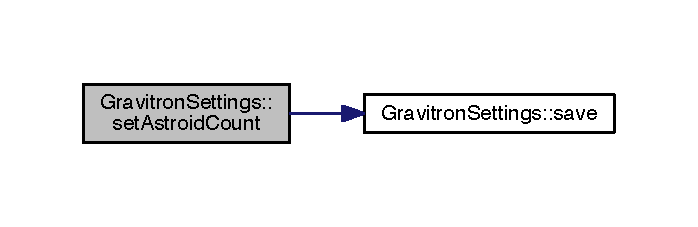
\includegraphics[width=335pt]{class_gravitron_settings_a0f48fe8d1d9fc850ac5272fffdc66c45_cgraph}
\end{center}
\end{figure}


\hypertarget{class_gravitron_settings_ac2ec7898b33cbd349497c59f69ee7c1d}{\index{Gravitron\+Settings@{Gravitron\+Settings}!set\+Bots\+Count@{set\+Bots\+Count}}
\index{set\+Bots\+Count@{set\+Bots\+Count}!Gravitron\+Settings@{Gravitron\+Settings}}
\subsubsection[{set\+Bots\+Count}]{\setlength{\rightskip}{0pt plus 5cm}void Gravitron\+Settings\+::set\+Bots\+Count (
\begin{DoxyParamCaption}
\item[{const int \&}]{source}
\end{DoxyParamCaption}
)}}\label{class_gravitron_settings_ac2ec7898b33cbd349497c59f69ee7c1d}


Here is the call graph for this function\+:\nopagebreak
\begin{figure}[H]
\begin{center}
\leavevmode
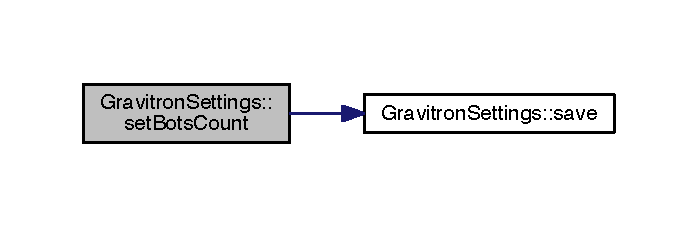
\includegraphics[width=335pt]{class_gravitron_settings_ac2ec7898b33cbd349497c59f69ee7c1d_cgraph}
\end{center}
\end{figure}


\hypertarget{class_gravitron_settings_ae8240cfb314457bd03e7053c0fe69aa3}{\index{Gravitron\+Settings@{Gravitron\+Settings}!set\+Difficulty@{set\+Difficulty}}
\index{set\+Difficulty@{set\+Difficulty}!Gravitron\+Settings@{Gravitron\+Settings}}
\subsubsection[{set\+Difficulty}]{\setlength{\rightskip}{0pt plus 5cm}void Gravitron\+Settings\+::set\+Difficulty (
\begin{DoxyParamCaption}
\item[{const int \&}]{source}
\end{DoxyParamCaption}
)}}\label{class_gravitron_settings_ae8240cfb314457bd03e7053c0fe69aa3}


Here is the call graph for this function\+:\nopagebreak
\begin{figure}[H]
\begin{center}
\leavevmode
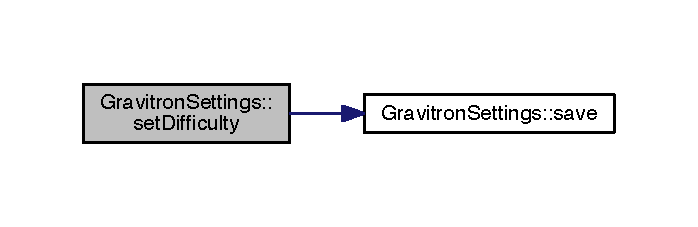
\includegraphics[width=335pt]{class_gravitron_settings_ae8240cfb314457bd03e7053c0fe69aa3_cgraph}
\end{center}
\end{figure}


\hypertarget{class_gravitron_settings_a68c312fe2c90b7aa39951751ffdc0be6}{\index{Gravitron\+Settings@{Gravitron\+Settings}!set\+Frag@{set\+Frag}}
\index{set\+Frag@{set\+Frag}!Gravitron\+Settings@{Gravitron\+Settings}}
\subsubsection[{set\+Frag}]{\setlength{\rightskip}{0pt plus 5cm}void Gravitron\+Settings\+::set\+Frag (
\begin{DoxyParamCaption}
\item[{const int \&}]{source}
\end{DoxyParamCaption}
)}}\label{class_gravitron_settings_a68c312fe2c90b7aa39951751ffdc0be6}


Here is the call graph for this function\+:\nopagebreak
\begin{figure}[H]
\begin{center}
\leavevmode
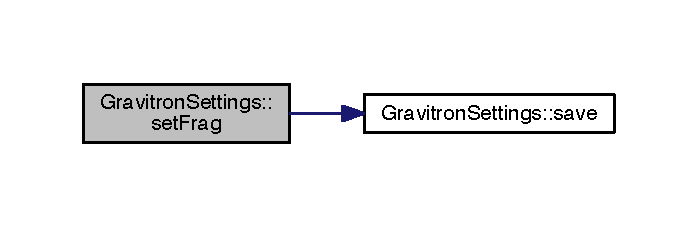
\includegraphics[width=335pt]{class_gravitron_settings_a68c312fe2c90b7aa39951751ffdc0be6_cgraph}
\end{center}
\end{figure}


\hypertarget{class_gravitron_settings_a63094c938fb60cc79ca096dd2444745a}{\index{Gravitron\+Settings@{Gravitron\+Settings}!set\+Full\+Screen@{set\+Full\+Screen}}
\index{set\+Full\+Screen@{set\+Full\+Screen}!Gravitron\+Settings@{Gravitron\+Settings}}
\subsubsection[{set\+Full\+Screen}]{\setlength{\rightskip}{0pt plus 5cm}void Gravitron\+Settings\+::set\+Full\+Screen (
\begin{DoxyParamCaption}
\item[{const bool \&}]{source}
\end{DoxyParamCaption}
)}}\label{class_gravitron_settings_a63094c938fb60cc79ca096dd2444745a}


Here is the call graph for this function\+:\nopagebreak
\begin{figure}[H]
\begin{center}
\leavevmode
\includegraphics[width=335pt]{class_gravitron_settings_a63094c938fb60cc79ca096dd2444745a_cgraph}
\end{center}
\end{figure}


\hypertarget{class_gravitron_settings_a1c457b47d88c01a5c3541f3c861fcda6}{\index{Gravitron\+Settings@{Gravitron\+Settings}!set\+Languare@{set\+Languare}}
\index{set\+Languare@{set\+Languare}!Gravitron\+Settings@{Gravitron\+Settings}}
\subsubsection[{set\+Languare}]{\setlength{\rightskip}{0pt plus 5cm}void Gravitron\+Settings\+::set\+Languare (
\begin{DoxyParamCaption}
\item[{const Q\+String \&}]{source}
\end{DoxyParamCaption}
)}}\label{class_gravitron_settings_a1c457b47d88c01a5c3541f3c861fcda6}


Here is the call graph for this function\+:\nopagebreak
\begin{figure}[H]
\begin{center}
\leavevmode
\includegraphics[width=335pt]{class_gravitron_settings_a1c457b47d88c01a5c3541f3c861fcda6_cgraph}
\end{center}
\end{figure}


\hypertarget{class_gravitron_settings_a19127cb8ad9035391cef6607ebfcfbd8}{\index{Gravitron\+Settings@{Gravitron\+Settings}!set\+Music\+Sound\+Volume@{set\+Music\+Sound\+Volume}}
\index{set\+Music\+Sound\+Volume@{set\+Music\+Sound\+Volume}!Gravitron\+Settings@{Gravitron\+Settings}}
\subsubsection[{set\+Music\+Sound\+Volume}]{\setlength{\rightskip}{0pt plus 5cm}void Gravitron\+Settings\+::set\+Music\+Sound\+Volume (
\begin{DoxyParamCaption}
\item[{const int \&}]{source}
\end{DoxyParamCaption}
)}}\label{class_gravitron_settings_a19127cb8ad9035391cef6607ebfcfbd8}


Here is the call graph for this function\+:\nopagebreak
\begin{figure}[H]
\begin{center}
\leavevmode
\includegraphics[width=350pt]{class_gravitron_settings_a19127cb8ad9035391cef6607ebfcfbd8_cgraph}
\end{center}
\end{figure}


\hypertarget{class_gravitron_settings_a27abb8747f90faa675cf875962a4cb17}{\index{Gravitron\+Settings@{Gravitron\+Settings}!set\+Network@{set\+Network}}
\index{set\+Network@{set\+Network}!Gravitron\+Settings@{Gravitron\+Settings}}
\subsubsection[{set\+Network}]{\setlength{\rightskip}{0pt plus 5cm}void Gravitron\+Settings\+::set\+Network (
\begin{DoxyParamCaption}
\item[{const bool \&}]{source}
\end{DoxyParamCaption}
)}}\label{class_gravitron_settings_a27abb8747f90faa675cf875962a4cb17}


Here is the call graph for this function\+:\nopagebreak
\begin{figure}[H]
\begin{center}
\leavevmode
\includegraphics[width=335pt]{class_gravitron_settings_a27abb8747f90faa675cf875962a4cb17_cgraph}
\end{center}
\end{figure}


\hypertarget{class_gravitron_settings_a1bb8463107c3236fd2610c657b4ffe59}{\index{Gravitron\+Settings@{Gravitron\+Settings}!set\+Planet\+Count@{set\+Planet\+Count}}
\index{set\+Planet\+Count@{set\+Planet\+Count}!Gravitron\+Settings@{Gravitron\+Settings}}
\subsubsection[{set\+Planet\+Count}]{\setlength{\rightskip}{0pt plus 5cm}void Gravitron\+Settings\+::set\+Planet\+Count (
\begin{DoxyParamCaption}
\item[{const int \&}]{source}
\end{DoxyParamCaption}
)}}\label{class_gravitron_settings_a1bb8463107c3236fd2610c657b4ffe59}


Here is the call graph for this function\+:\nopagebreak
\begin{figure}[H]
\begin{center}
\leavevmode
\includegraphics[width=335pt]{class_gravitron_settings_a1bb8463107c3236fd2610c657b4ffe59_cgraph}
\end{center}
\end{figure}


\hypertarget{class_gravitron_settings_ac6dc8d0025905248e80217198513a044}{\index{Gravitron\+Settings@{Gravitron\+Settings}!set\+Player\+Name@{set\+Player\+Name}}
\index{set\+Player\+Name@{set\+Player\+Name}!Gravitron\+Settings@{Gravitron\+Settings}}
\subsubsection[{set\+Player\+Name}]{\setlength{\rightskip}{0pt plus 5cm}void Gravitron\+Settings\+::set\+Player\+Name (
\begin{DoxyParamCaption}
\item[{const Q\+String \&}]{source}
\end{DoxyParamCaption}
)}}\label{class_gravitron_settings_ac6dc8d0025905248e80217198513a044}


Here is the call graph for this function\+:\nopagebreak
\begin{figure}[H]
\begin{center}
\leavevmode
\includegraphics[width=335pt]{class_gravitron_settings_ac6dc8d0025905248e80217198513a044_cgraph}
\end{center}
\end{figure}


\hypertarget{class_gravitron_settings_aaceaf8068d09b9e22d8085c6ca3db2d8}{\index{Gravitron\+Settings@{Gravitron\+Settings}!set\+Playing\+Field\+Size@{set\+Playing\+Field\+Size}}
\index{set\+Playing\+Field\+Size@{set\+Playing\+Field\+Size}!Gravitron\+Settings@{Gravitron\+Settings}}
\subsubsection[{set\+Playing\+Field\+Size}]{\setlength{\rightskip}{0pt plus 5cm}void Gravitron\+Settings\+::set\+Playing\+Field\+Size (
\begin{DoxyParamCaption}
\item[{const int \&}]{source}
\end{DoxyParamCaption}
)}}\label{class_gravitron_settings_aaceaf8068d09b9e22d8085c6ca3db2d8}


Here is the call graph for this function\+:\nopagebreak
\begin{figure}[H]
\begin{center}
\leavevmode
\includegraphics[width=339pt]{class_gravitron_settings_aaceaf8068d09b9e22d8085c6ca3db2d8_cgraph}
\end{center}
\end{figure}


\hypertarget{class_gravitron_settings_afcaa509baf03618793cc7fcfb5ef2030}{\index{Gravitron\+Settings@{Gravitron\+Settings}!set\+Play\+Music@{set\+Play\+Music}}
\index{set\+Play\+Music@{set\+Play\+Music}!Gravitron\+Settings@{Gravitron\+Settings}}
\subsubsection[{set\+Play\+Music}]{\setlength{\rightskip}{0pt plus 5cm}void Gravitron\+Settings\+::set\+Play\+Music (
\begin{DoxyParamCaption}
\item[{const bool \&}]{source}
\end{DoxyParamCaption}
)}}\label{class_gravitron_settings_afcaa509baf03618793cc7fcfb5ef2030}


Here is the call graph for this function\+:\nopagebreak
\begin{figure}[H]
\begin{center}
\leavevmode
\includegraphics[width=335pt]{class_gravitron_settings_afcaa509baf03618793cc7fcfb5ef2030_cgraph}
\end{center}
\end{figure}


\hypertarget{class_gravitron_settings_a658374f96e4bb64f91e770a6df87cc69}{\index{Gravitron\+Settings@{Gravitron\+Settings}!set\+Play\+Sounds@{set\+Play\+Sounds}}
\index{set\+Play\+Sounds@{set\+Play\+Sounds}!Gravitron\+Settings@{Gravitron\+Settings}}
\subsubsection[{set\+Play\+Sounds}]{\setlength{\rightskip}{0pt plus 5cm}void Gravitron\+Settings\+::set\+Play\+Sounds (
\begin{DoxyParamCaption}
\item[{const bool \&}]{source}
\end{DoxyParamCaption}
)}}\label{class_gravitron_settings_a658374f96e4bb64f91e770a6df87cc69}


Here is the call graph for this function\+:\nopagebreak
\begin{figure}[H]
\begin{center}
\leavevmode
\includegraphics[width=335pt]{class_gravitron_settings_a658374f96e4bb64f91e770a6df87cc69_cgraph}
\end{center}
\end{figure}


\hypertarget{class_gravitron_settings_a4263bace900a630e49d498114102b181}{\index{Gravitron\+Settings@{Gravitron\+Settings}!set\+Respaw\+Time@{set\+Respaw\+Time}}
\index{set\+Respaw\+Time@{set\+Respaw\+Time}!Gravitron\+Settings@{Gravitron\+Settings}}
\subsubsection[{set\+Respaw\+Time}]{\setlength{\rightskip}{0pt plus 5cm}void Gravitron\+Settings\+::set\+Respaw\+Time (
\begin{DoxyParamCaption}
\item[{const int \&}]{source}
\end{DoxyParamCaption}
)}}\label{class_gravitron_settings_a4263bace900a630e49d498114102b181}


Here is the call graph for this function\+:\nopagebreak
\begin{figure}[H]
\begin{center}
\leavevmode
\includegraphics[width=335pt]{class_gravitron_settings_a4263bace900a630e49d498114102b181_cgraph}
\end{center}
\end{figure}




\subsection{Friends And Related Function Documentation}
\hypertarget{class_gravitron_settings_a24a8274b8fa276e0da0ebf0e6fc3d176}{\index{Gravitron\+Settings@{Gravitron\+Settings}!operator$<$$<$@{operator$<$$<$}}
\index{operator$<$$<$@{operator$<$$<$}!Gravitron\+Settings@{Gravitron\+Settings}}
\subsubsection[{operator$<$$<$}]{\setlength{\rightskip}{0pt plus 5cm}Q\+Data\+Stream\& operator$<$$<$ (
\begin{DoxyParamCaption}
\item[{Q\+Data\+Stream \&}]{stream, }
\item[{const {\bf Gravitron\+Settings} \&}]{settings}
\end{DoxyParamCaption}
)\hspace{0.3cm}{\ttfamily [friend]}}}\label{class_gravitron_settings_a24a8274b8fa276e0da0ebf0e6fc3d176}
\hypertarget{class_gravitron_settings_a652a2b630485f03a4a527ef3ef7a3367}{\index{Gravitron\+Settings@{Gravitron\+Settings}!operator$>$$>$@{operator$>$$>$}}
\index{operator$>$$>$@{operator$>$$>$}!Gravitron\+Settings@{Gravitron\+Settings}}
\subsubsection[{operator$>$$>$}]{\setlength{\rightskip}{0pt plus 5cm}Q\+Data\+Stream\& operator$>$$>$ (
\begin{DoxyParamCaption}
\item[{Q\+Data\+Stream \&}]{stream, }
\item[{{\bf Gravitron\+Settings} \&}]{settings}
\end{DoxyParamCaption}
)\hspace{0.3cm}{\ttfamily [friend]}}}\label{class_gravitron_settings_a652a2b630485f03a4a527ef3ef7a3367}


The documentation for this class was generated from the following files\+:\begin{DoxyCompactItemize}
\item 
src/headers/\hyperlink{_gravitron_settings_8h}{Gravitron\+Settings.\+h}\item 
src/\hyperlink{_gravitron_settings_8cpp}{Gravitron\+Settings.\+cpp}\end{DoxyCompactItemize}

\hypertarget{class_human_network_player}{\section{Human\+Network\+Player Class Reference}
\label{class_human_network_player}\index{Human\+Network\+Player@{Human\+Network\+Player}}
}


{\ttfamily \#include $<$Human\+Network\+Player.\+h$>$}



Inheritance diagram for Human\+Network\+Player\+:\nopagebreak
\begin{figure}[H]
\begin{center}
\leavevmode
\includegraphics[width=193pt]{class_human_network_player__inherit__graph}
\end{center}
\end{figure}


Collaboration diagram for Human\+Network\+Player\+:\nopagebreak
\begin{figure}[H]
\begin{center}
\leavevmode
\includegraphics[width=267pt]{class_human_network_player__coll__graph}
\end{center}
\end{figure}
\subsection*{Public Member Functions}
\begin{DoxyCompactItemize}
\item 
\hyperlink{class_human_network_player_a2d77b83c604f55e401e32f5cb3c8023a}{Human\+Network\+Player} (\hyperlink{class_spacecraft}{Spacecraft} $\ast$\hyperlink{class_player_a7cc88a054d2329b1ca7472a86b2030ca}{spacecraft}, int \hyperlink{class_player_a9528a6db252f2fe947fd7d9189837aec}{frag}, \hyperlink{class_tcp_server}{Tcp\+Server} $\ast$server)
\item 
virtual \hyperlink{class_human_network_player_ab8d3f49f7ab1c7157efdd0b949a52045}{$\sim$\+Human\+Network\+Player} ()
\item 
void \hyperlink{class_human_network_player_a3914e46fec4bd007fff44ec984599d94}{process\+Input} ()
\end{DoxyCompactItemize}
\subsection*{Protected Member Functions}
\begin{DoxyCompactItemize}
\item 
virtual void \hyperlink{class_human_network_player_a6faa3112587ecc9b16caa28782682976}{exec\+Action} (int code)
\end{DoxyCompactItemize}
\subsection*{Additional Inherited Members}


\subsection{Constructor \& Destructor Documentation}
\hypertarget{class_human_network_player_a2d77b83c604f55e401e32f5cb3c8023a}{\index{Human\+Network\+Player@{Human\+Network\+Player}!Human\+Network\+Player@{Human\+Network\+Player}}
\index{Human\+Network\+Player@{Human\+Network\+Player}!Human\+Network\+Player@{Human\+Network\+Player}}
\subsubsection[{Human\+Network\+Player}]{\setlength{\rightskip}{0pt plus 5cm}Human\+Network\+Player\+::\+Human\+Network\+Player (
\begin{DoxyParamCaption}
\item[{{\bf Spacecraft} $\ast$}]{spacecraft, }
\item[{int}]{frag, }
\item[{{\bf Tcp\+Server} $\ast$}]{server}
\end{DoxyParamCaption}
)}}\label{class_human_network_player_a2d77b83c604f55e401e32f5cb3c8023a}
\hypertarget{class_human_network_player_ab8d3f49f7ab1c7157efdd0b949a52045}{\index{Human\+Network\+Player@{Human\+Network\+Player}!````~Human\+Network\+Player@{$\sim$\+Human\+Network\+Player}}
\index{````~Human\+Network\+Player@{$\sim$\+Human\+Network\+Player}!Human\+Network\+Player@{Human\+Network\+Player}}
\subsubsection[{$\sim$\+Human\+Network\+Player}]{\setlength{\rightskip}{0pt plus 5cm}Human\+Network\+Player\+::$\sim$\+Human\+Network\+Player (
\begin{DoxyParamCaption}
{}
\end{DoxyParamCaption}
)\hspace{0.3cm}{\ttfamily [virtual]}}}\label{class_human_network_player_ab8d3f49f7ab1c7157efdd0b949a52045}


\subsection{Member Function Documentation}
\hypertarget{class_human_network_player_a6faa3112587ecc9b16caa28782682976}{\index{Human\+Network\+Player@{Human\+Network\+Player}!exec\+Action@{exec\+Action}}
\index{exec\+Action@{exec\+Action}!Human\+Network\+Player@{Human\+Network\+Player}}
\subsubsection[{exec\+Action}]{\setlength{\rightskip}{0pt plus 5cm}void Human\+Network\+Player\+::exec\+Action (
\begin{DoxyParamCaption}
\item[{int}]{code}
\end{DoxyParamCaption}
)\hspace{0.3cm}{\ttfamily [protected]}, {\ttfamily [virtual]}}}\label{class_human_network_player_a6faa3112587ecc9b16caa28782682976}


Reimplemented from \hyperlink{class_human_player_a1fac561ab5995308892dd237b3b32645}{Human\+Player}.



Here is the call graph for this function\+:\nopagebreak
\begin{figure}[H]
\begin{center}
\leavevmode
\includegraphics[width=350pt]{class_human_network_player_a6faa3112587ecc9b16caa28782682976_cgraph}
\end{center}
\end{figure}


\hypertarget{class_human_network_player_a3914e46fec4bd007fff44ec984599d94}{\index{Human\+Network\+Player@{Human\+Network\+Player}!process\+Input@{process\+Input}}
\index{process\+Input@{process\+Input}!Human\+Network\+Player@{Human\+Network\+Player}}
\subsubsection[{process\+Input}]{\setlength{\rightskip}{0pt plus 5cm}void Human\+Network\+Player\+::process\+Input (
\begin{DoxyParamCaption}
{}
\end{DoxyParamCaption}
)\hspace{0.3cm}{\ttfamily [virtual]}}}\label{class_human_network_player_a3914e46fec4bd007fff44ec984599d94}


Reimplemented from \hyperlink{class_human_player_a4298cb4a77be8ef79cc289baec199602}{Human\+Player}.



Here is the call graph for this function\+:\nopagebreak
\begin{figure}[H]
\begin{center}
\leavevmode
\includegraphics[width=350pt]{class_human_network_player_a3914e46fec4bd007fff44ec984599d94_cgraph}
\end{center}
\end{figure}




The documentation for this class was generated from the following files\+:\begin{DoxyCompactItemize}
\item 
src/headers/\hyperlink{_human_network_player_8h}{Human\+Network\+Player.\+h}\item 
src/\hyperlink{_human_network_player_8cpp}{Human\+Network\+Player.\+cpp}\end{DoxyCompactItemize}

\hypertarget{class_human_player}{\section{Human\+Player Class Reference}
\label{class_human_player}\index{Human\+Player@{Human\+Player}}
}


{\ttfamily \#include $<$Human\+Player.\+h$>$}



Inheritance diagram for Human\+Player\+:\nopagebreak
\begin{figure}[H]
\begin{center}
\leavevmode
\includegraphics[width=193pt]{class_human_player__inherit__graph}
\end{center}
\end{figure}


Collaboration diagram for Human\+Player\+:\nopagebreak
\begin{figure}[H]
\begin{center}
\leavevmode
\includegraphics[width=264pt]{class_human_player__coll__graph}
\end{center}
\end{figure}
\subsection*{Public Member Functions}
\begin{DoxyCompactItemize}
\item 
\hyperlink{class_human_player_aed948852b858c81d6ce6dbc2c16fe4ca}{Human\+Player} (\hyperlink{class_spacecraft}{Spacecraft} $\ast$\hyperlink{class_player_a7cc88a054d2329b1ca7472a86b2030ca}{spacecraft}, int \hyperlink{class_player_a9528a6db252f2fe947fd7d9189837aec}{frag})
\item 
virtual \hyperlink{class_human_player_abdeb9d120fc74c8d82ec0c688883f16f}{$\sim$\+Human\+Player} ()
\item 
virtual void \hyperlink{class_human_player_a4298cb4a77be8ef79cc289baec199602}{process\+Input} ()
\end{DoxyCompactItemize}
\subsection*{Protected Member Functions}
\begin{DoxyCompactItemize}
\item 
virtual void \hyperlink{class_human_player_a1fac561ab5995308892dd237b3b32645}{exec\+Action} (int code)
\end{DoxyCompactItemize}
\subsection*{Protected Attributes}
\begin{DoxyCompactItemize}
\item 
Q\+Object $\ast$ \hyperlink{class_human_player_afac1bdc1194ebbd2236d0df12a1fb341}{input\+Handler}
\end{DoxyCompactItemize}


\subsection{Constructor \& Destructor Documentation}
\hypertarget{class_human_player_aed948852b858c81d6ce6dbc2c16fe4ca}{\index{Human\+Player@{Human\+Player}!Human\+Player@{Human\+Player}}
\index{Human\+Player@{Human\+Player}!Human\+Player@{Human\+Player}}
\subsubsection[{Human\+Player}]{\setlength{\rightskip}{0pt plus 5cm}Human\+Player\+::\+Human\+Player (
\begin{DoxyParamCaption}
\item[{{\bf Spacecraft} $\ast$}]{spacecraft, }
\item[{int}]{frag}
\end{DoxyParamCaption}
)}}\label{class_human_player_aed948852b858c81d6ce6dbc2c16fe4ca}
\hypertarget{class_human_player_abdeb9d120fc74c8d82ec0c688883f16f}{\index{Human\+Player@{Human\+Player}!````~Human\+Player@{$\sim$\+Human\+Player}}
\index{````~Human\+Player@{$\sim$\+Human\+Player}!Human\+Player@{Human\+Player}}
\subsubsection[{$\sim$\+Human\+Player}]{\setlength{\rightskip}{0pt plus 5cm}Human\+Player\+::$\sim$\+Human\+Player (
\begin{DoxyParamCaption}
{}
\end{DoxyParamCaption}
)\hspace{0.3cm}{\ttfamily [virtual]}}}\label{class_human_player_abdeb9d120fc74c8d82ec0c688883f16f}


\subsection{Member Function Documentation}
\hypertarget{class_human_player_a1fac561ab5995308892dd237b3b32645}{\index{Human\+Player@{Human\+Player}!exec\+Action@{exec\+Action}}
\index{exec\+Action@{exec\+Action}!Human\+Player@{Human\+Player}}
\subsubsection[{exec\+Action}]{\setlength{\rightskip}{0pt plus 5cm}void Human\+Player\+::exec\+Action (
\begin{DoxyParamCaption}
\item[{int}]{code}
\end{DoxyParamCaption}
)\hspace{0.3cm}{\ttfamily [protected]}, {\ttfamily [virtual]}}}\label{class_human_player_a1fac561ab5995308892dd237b3b32645}


Reimplemented in \hyperlink{class_human_network_player_a6faa3112587ecc9b16caa28782682976}{Human\+Network\+Player}.



Here is the call graph for this function\+:\nopagebreak
\begin{figure}[H]
\begin{center}
\leavevmode
\includegraphics[width=350pt]{class_human_player_a1fac561ab5995308892dd237b3b32645_cgraph}
\end{center}
\end{figure}


\hypertarget{class_human_player_a4298cb4a77be8ef79cc289baec199602}{\index{Human\+Player@{Human\+Player}!process\+Input@{process\+Input}}
\index{process\+Input@{process\+Input}!Human\+Player@{Human\+Player}}
\subsubsection[{process\+Input}]{\setlength{\rightskip}{0pt plus 5cm}void Human\+Player\+::process\+Input (
\begin{DoxyParamCaption}
{}
\end{DoxyParamCaption}
)\hspace{0.3cm}{\ttfamily [virtual]}}}\label{class_human_player_a4298cb4a77be8ef79cc289baec199602}


Reimplemented from \hyperlink{class_player_ab8afa8b779cc8b9defcb232e8365d556}{Player}.



Reimplemented in \hyperlink{class_human_network_player_a3914e46fec4bd007fff44ec984599d94}{Human\+Network\+Player}.



Here is the call graph for this function\+:\nopagebreak
\begin{figure}[H]
\begin{center}
\leavevmode
\includegraphics[width=350pt]{class_human_player_a4298cb4a77be8ef79cc289baec199602_cgraph}
\end{center}
\end{figure}




\subsection{Member Data Documentation}
\hypertarget{class_human_player_afac1bdc1194ebbd2236d0df12a1fb341}{\index{Human\+Player@{Human\+Player}!input\+Handler@{input\+Handler}}
\index{input\+Handler@{input\+Handler}!Human\+Player@{Human\+Player}}
\subsubsection[{input\+Handler}]{\setlength{\rightskip}{0pt plus 5cm}Q\+Object$\ast$ Human\+Player\+::input\+Handler\hspace{0.3cm}{\ttfamily [protected]}}}\label{class_human_player_afac1bdc1194ebbd2236d0df12a1fb341}


The documentation for this class was generated from the following files\+:\begin{DoxyCompactItemize}
\item 
src/headers/\hyperlink{_human_player_8h}{Human\+Player.\+h}\item 
src/\hyperlink{_human_player_8cpp}{Human\+Player.\+cpp}\end{DoxyCompactItemize}

\hypertarget{class_input_handler}{\section{Input\+Handler Class Reference}
\label{class_input_handler}\index{Input\+Handler@{Input\+Handler}}
}


{\ttfamily \#include $<$Input\+Handler.\+h$>$}



Inheritance diagram for Input\+Handler\+:\nopagebreak
\begin{figure}[H]
\begin{center}
\leavevmode
\includegraphics[width=153pt]{class_input_handler__inherit__graph}
\end{center}
\end{figure}


Collaboration diagram for Input\+Handler\+:\nopagebreak
\begin{figure}[H]
\begin{center}
\leavevmode
\includegraphics[width=153pt]{class_input_handler__coll__graph}
\end{center}
\end{figure}
\subsection*{Signals}
\begin{DoxyCompactItemize}
\item 
void \hyperlink{class_input_handler_a13835fb9eeeeafd790b37c0fff595047}{inputs\+Changed} (set$<$ int $>$ inputs)
\end{DoxyCompactItemize}
\subsection*{Public Member Functions}
\begin{DoxyCompactItemize}
\item 
\hyperlink{class_input_handler_a698aa4af4f326a9881835fda251ca996}{Input\+Handler} ()
\item 
set$<$ int $>$ \hyperlink{class_input_handler_a2c60f224394c42a36310cfdde57f09c3}{get\+Inputs} ()
\item 
void \hyperlink{class_input_handler_ac384ab20e654c7a850e79266d67bde2d}{remove\+Input\+Code} (int code)
\item 
void \hyperlink{class_input_handler_a81337e17ca813af525efcc257c644a09}{insert\+Input\+Code} (int code)
\end{DoxyCompactItemize}
\subsection*{Protected Member Functions}
\begin{DoxyCompactItemize}
\item 
bool \hyperlink{class_input_handler_a90dcf6f91f3441a8e99d082cb8696ddf}{event\+Filter} (Q\+Object $\ast$obj, Q\+Event $\ast$event)
\end{DoxyCompactItemize}


\subsection{Constructor \& Destructor Documentation}
\hypertarget{class_input_handler_a698aa4af4f326a9881835fda251ca996}{\index{Input\+Handler@{Input\+Handler}!Input\+Handler@{Input\+Handler}}
\index{Input\+Handler@{Input\+Handler}!Input\+Handler@{Input\+Handler}}
\subsubsection[{Input\+Handler}]{\setlength{\rightskip}{0pt plus 5cm}Input\+Handler\+::\+Input\+Handler (
\begin{DoxyParamCaption}
{}
\end{DoxyParamCaption}
)}}\label{class_input_handler_a698aa4af4f326a9881835fda251ca996}


\subsection{Member Function Documentation}
\hypertarget{class_input_handler_a90dcf6f91f3441a8e99d082cb8696ddf}{\index{Input\+Handler@{Input\+Handler}!event\+Filter@{event\+Filter}}
\index{event\+Filter@{event\+Filter}!Input\+Handler@{Input\+Handler}}
\subsubsection[{event\+Filter}]{\setlength{\rightskip}{0pt plus 5cm}bool Input\+Handler\+::event\+Filter (
\begin{DoxyParamCaption}
\item[{Q\+Object $\ast$}]{obj, }
\item[{Q\+Event $\ast$}]{event}
\end{DoxyParamCaption}
)\hspace{0.3cm}{\ttfamily [protected]}}}\label{class_input_handler_a90dcf6f91f3441a8e99d082cb8696ddf}
\hypertarget{class_input_handler_a2c60f224394c42a36310cfdde57f09c3}{\index{Input\+Handler@{Input\+Handler}!get\+Inputs@{get\+Inputs}}
\index{get\+Inputs@{get\+Inputs}!Input\+Handler@{Input\+Handler}}
\subsubsection[{get\+Inputs}]{\setlength{\rightskip}{0pt plus 5cm}set$<$ int $>$ Input\+Handler\+::get\+Inputs (
\begin{DoxyParamCaption}
{}
\end{DoxyParamCaption}
)}}\label{class_input_handler_a2c60f224394c42a36310cfdde57f09c3}
\hypertarget{class_input_handler_a13835fb9eeeeafd790b37c0fff595047}{\index{Input\+Handler@{Input\+Handler}!inputs\+Changed@{inputs\+Changed}}
\index{inputs\+Changed@{inputs\+Changed}!Input\+Handler@{Input\+Handler}}
\subsubsection[{inputs\+Changed}]{\setlength{\rightskip}{0pt plus 5cm}void Input\+Handler\+::inputs\+Changed (
\begin{DoxyParamCaption}
\item[{set$<$ int $>$}]{inputs}
\end{DoxyParamCaption}
)\hspace{0.3cm}{\ttfamily [signal]}}}\label{class_input_handler_a13835fb9eeeeafd790b37c0fff595047}
\hypertarget{class_input_handler_a81337e17ca813af525efcc257c644a09}{\index{Input\+Handler@{Input\+Handler}!insert\+Input\+Code@{insert\+Input\+Code}}
\index{insert\+Input\+Code@{insert\+Input\+Code}!Input\+Handler@{Input\+Handler}}
\subsubsection[{insert\+Input\+Code}]{\setlength{\rightskip}{0pt plus 5cm}void Input\+Handler\+::insert\+Input\+Code (
\begin{DoxyParamCaption}
\item[{int}]{code}
\end{DoxyParamCaption}
)}}\label{class_input_handler_a81337e17ca813af525efcc257c644a09}
\hypertarget{class_input_handler_ac384ab20e654c7a850e79266d67bde2d}{\index{Input\+Handler@{Input\+Handler}!remove\+Input\+Code@{remove\+Input\+Code}}
\index{remove\+Input\+Code@{remove\+Input\+Code}!Input\+Handler@{Input\+Handler}}
\subsubsection[{remove\+Input\+Code}]{\setlength{\rightskip}{0pt plus 5cm}void Input\+Handler\+::remove\+Input\+Code (
\begin{DoxyParamCaption}
\item[{int}]{code}
\end{DoxyParamCaption}
)}}\label{class_input_handler_ac384ab20e654c7a850e79266d67bde2d}


The documentation for this class was generated from the following files\+:\begin{DoxyCompactItemize}
\item 
src/headers/\hyperlink{_input_handler_8h}{Input\+Handler.\+h}\item 
src/\hyperlink{_input_handler_8cpp}{Input\+Handler.\+cpp}\end{DoxyCompactItemize}

\hypertarget{class_laser}{\section{Laser Class Reference}
\label{class_laser}\index{Laser@{Laser}}
}


{\ttfamily \#include $<$Laser.\+h$>$}



Inheritance diagram for Laser\+:\nopagebreak
\begin{figure}[H]
\begin{center}
\leavevmode
\includegraphics[width=147pt]{class_laser__inherit__graph}
\end{center}
\end{figure}


Collaboration diagram for Laser\+:\nopagebreak
\begin{figure}[H]
\begin{center}
\leavevmode
\includegraphics[width=231pt]{class_laser__coll__graph}
\end{center}
\end{figure}
\subsection*{Public Member Functions}
\begin{DoxyCompactItemize}
\item 
\hyperlink{class_laser_a68465e89283dffcc29a37e94693c6f87}{Laser} ()
\item 
\hyperlink{class_laser_a326b845c80bcf384cd91452364805d4d}{Laser} (\hyperlink{class_vec3f}{Vec3f} \hyperlink{class_game_actor_aefed3c91bf32ad388d86657b3bb9ddfa}{position}, \hyperlink{class_vec3f}{Vec3f} \hyperlink{class_game_actor_a95518bf01411eafe983df8815e8682d1}{velocity}, \hyperlink{class_game_field}{Game\+Field} \&\hyperlink{class_game_actor_a0224fbc502abd6b7579787aa234332d5}{field}, \hyperlink{class_game_actor}{Game\+Actor} \&\hyperlink{class_projectile_a54dec73f149e6619fac8f5cf8910edcc}{friendly}, vector$<$ \hyperlink{class_game_actor}{Game\+Actor} $\ast$ $>$ $\ast$\hyperlink{class_game_actor_a2405618d895f5143b42ae9e94d20e693}{actors})
\item 
\hyperlink{class_laser_abcdb5d7610f089ddee97c9d512892ce7}{Laser} (\hyperlink{class_game_actor}{Game\+Actor} \&actor, \hyperlink{class_vec3f}{Vec3f} \hyperlink{class_game_actor_a95518bf01411eafe983df8815e8682d1}{velocity}, \hyperlink{class_game_field}{Game\+Field} \&\hyperlink{class_game_actor_a0224fbc502abd6b7579787aa234332d5}{field}, \hyperlink{class_game_actor}{Game\+Actor} \&\hyperlink{class_projectile_a54dec73f149e6619fac8f5cf8910edcc}{friendly}, vector$<$ \hyperlink{class_game_actor}{Game\+Actor} $\ast$ $>$ $\ast$\hyperlink{class_game_actor_a2405618d895f5143b42ae9e94d20e693}{actors})
\item 
\hyperlink{class_laser_ac8b00c242912954900642b341d6e7337}{Laser} (\hyperlink{class_game_actor}{Game\+Actor} \&actor, \hyperlink{class_game_field}{Game\+Field} \&\hyperlink{class_game_actor_a0224fbc502abd6b7579787aa234332d5}{field}, \hyperlink{class_game_actor}{Game\+Actor} \&\hyperlink{class_projectile_a54dec73f149e6619fac8f5cf8910edcc}{friendly}, vector$<$ \hyperlink{class_game_actor}{Game\+Actor} $\ast$ $>$ $\ast$\hyperlink{class_game_actor_a2405618d895f5143b42ae9e94d20e693}{actors})
\item 
\hyperlink{class_laser_a46c640df78e3ee5c367216a5306cfc5c}{Laser} (const \hyperlink{class_laser}{Laser} \&laser)
\item 
\hyperlink{class_laser_aa9baee5ed9775426e0b1d563c4687711}{$\sim$\+Laser} ()
\item 
int \hyperlink{class_laser_ae1d4d2df6586402139d480a9c5324610}{get\+Time\+To\+Live} () const 
\item 
void \hyperlink{class_laser_a6c26eb024fd0ae01920c299d1af2679d}{handle\+Collision} (\hyperlink{class_game_actor}{Game\+Actor} \&other) override
\item 
\hyperlink{class_game_actor_view}{Game\+Actor\+View} $\ast$ \hyperlink{class_laser_af00728fe7cabd4f63cb5ce66f4c50e86}{get\+View} () const override
\end{DoxyCompactItemize}
\subsection*{Additional Inherited Members}


\subsection{Constructor \& Destructor Documentation}
\hypertarget{class_laser_a68465e89283dffcc29a37e94693c6f87}{\index{Laser@{Laser}!Laser@{Laser}}
\index{Laser@{Laser}!Laser@{Laser}}
\subsubsection[{Laser}]{\setlength{\rightskip}{0pt plus 5cm}Laser\+::\+Laser (
\begin{DoxyParamCaption}
{}
\end{DoxyParamCaption}
)}}\label{class_laser_a68465e89283dffcc29a37e94693c6f87}
\hypertarget{class_laser_a326b845c80bcf384cd91452364805d4d}{\index{Laser@{Laser}!Laser@{Laser}}
\index{Laser@{Laser}!Laser@{Laser}}
\subsubsection[{Laser}]{\setlength{\rightskip}{0pt plus 5cm}Laser\+::\+Laser (
\begin{DoxyParamCaption}
\item[{{\bf Vec3f}}]{position, }
\item[{{\bf Vec3f}}]{velocity, }
\item[{{\bf Game\+Field} \&}]{field, }
\item[{{\bf Game\+Actor} \&}]{friendly, }
\item[{vector$<$ {\bf Game\+Actor} $\ast$ $>$ $\ast$}]{actors}
\end{DoxyParamCaption}
)}}\label{class_laser_a326b845c80bcf384cd91452364805d4d}


Here is the call graph for this function\+:\nopagebreak
\begin{figure}[H]
\begin{center}
\leavevmode
\includegraphics[width=309pt]{class_laser_a326b845c80bcf384cd91452364805d4d_cgraph}
\end{center}
\end{figure}


\hypertarget{class_laser_abcdb5d7610f089ddee97c9d512892ce7}{\index{Laser@{Laser}!Laser@{Laser}}
\index{Laser@{Laser}!Laser@{Laser}}
\subsubsection[{Laser}]{\setlength{\rightskip}{0pt plus 5cm}Laser\+::\+Laser (
\begin{DoxyParamCaption}
\item[{{\bf Game\+Actor} \&}]{actor, }
\item[{{\bf Vec3f}}]{velocity, }
\item[{{\bf Game\+Field} \&}]{field, }
\item[{{\bf Game\+Actor} \&}]{friendly, }
\item[{vector$<$ {\bf Game\+Actor} $\ast$ $>$ $\ast$}]{actors}
\end{DoxyParamCaption}
)}}\label{class_laser_abcdb5d7610f089ddee97c9d512892ce7}


Here is the call graph for this function\+:\nopagebreak
\begin{figure}[H]
\begin{center}
\leavevmode
\includegraphics[width=309pt]{class_laser_abcdb5d7610f089ddee97c9d512892ce7_cgraph}
\end{center}
\end{figure}


\hypertarget{class_laser_ac8b00c242912954900642b341d6e7337}{\index{Laser@{Laser}!Laser@{Laser}}
\index{Laser@{Laser}!Laser@{Laser}}
\subsubsection[{Laser}]{\setlength{\rightskip}{0pt plus 5cm}Laser\+::\+Laser (
\begin{DoxyParamCaption}
\item[{{\bf Game\+Actor} \&}]{actor, }
\item[{{\bf Game\+Field} \&}]{field, }
\item[{{\bf Game\+Actor} \&}]{friendly, }
\item[{vector$<$ {\bf Game\+Actor} $\ast$ $>$ $\ast$}]{actors}
\end{DoxyParamCaption}
)}}\label{class_laser_ac8b00c242912954900642b341d6e7337}


Here is the call graph for this function\+:\nopagebreak
\begin{figure}[H]
\begin{center}
\leavevmode
\includegraphics[width=309pt]{class_laser_ac8b00c242912954900642b341d6e7337_cgraph}
\end{center}
\end{figure}


\hypertarget{class_laser_a46c640df78e3ee5c367216a5306cfc5c}{\index{Laser@{Laser}!Laser@{Laser}}
\index{Laser@{Laser}!Laser@{Laser}}
\subsubsection[{Laser}]{\setlength{\rightskip}{0pt plus 5cm}Laser\+::\+Laser (
\begin{DoxyParamCaption}
\item[{const {\bf Laser} \&}]{laser}
\end{DoxyParamCaption}
)}}\label{class_laser_a46c640df78e3ee5c367216a5306cfc5c}
\hypertarget{class_laser_aa9baee5ed9775426e0b1d563c4687711}{\index{Laser@{Laser}!````~Laser@{$\sim$\+Laser}}
\index{````~Laser@{$\sim$\+Laser}!Laser@{Laser}}
\subsubsection[{$\sim$\+Laser}]{\setlength{\rightskip}{0pt plus 5cm}Laser\+::$\sim$\+Laser (
\begin{DoxyParamCaption}
{}
\end{DoxyParamCaption}
)}}\label{class_laser_aa9baee5ed9775426e0b1d563c4687711}


\subsection{Member Function Documentation}
\hypertarget{class_laser_ae1d4d2df6586402139d480a9c5324610}{\index{Laser@{Laser}!get\+Time\+To\+Live@{get\+Time\+To\+Live}}
\index{get\+Time\+To\+Live@{get\+Time\+To\+Live}!Laser@{Laser}}
\subsubsection[{get\+Time\+To\+Live}]{\setlength{\rightskip}{0pt plus 5cm}int Laser\+::get\+Time\+To\+Live (
\begin{DoxyParamCaption}
{}
\end{DoxyParamCaption}
) const}}\label{class_laser_ae1d4d2df6586402139d480a9c5324610}
\hypertarget{class_laser_af00728fe7cabd4f63cb5ce66f4c50e86}{\index{Laser@{Laser}!get\+View@{get\+View}}
\index{get\+View@{get\+View}!Laser@{Laser}}
\subsubsection[{get\+View}]{\setlength{\rightskip}{0pt plus 5cm}{\bf Game\+Actor\+View} $\ast$ Laser\+::get\+View (
\begin{DoxyParamCaption}
{}
\end{DoxyParamCaption}
) const\hspace{0.3cm}{\ttfamily [override]}, {\ttfamily [virtual]}}}\label{class_laser_af00728fe7cabd4f63cb5ce66f4c50e86}
Creates and returns a \hyperlink{class_game_actor_view}{Game\+Actor\+View} of this instance of \hyperlink{class_game_actor}{Game\+Actor}. \begin{DoxyReturn}{Returns}
the \hyperlink{class_game_actor_view}{Game\+Actor\+View} for this \hyperlink{class_game_actor}{Game\+Actor} 
\end{DoxyReturn}


Reimplemented from \hyperlink{class_game_actor_ae63b522db0d88f56e3c7a8cfb60d31a6}{Game\+Actor}.



Here is the call graph for this function\+:\nopagebreak
\begin{figure}[H]
\begin{center}
\leavevmode
\includegraphics[width=350pt]{class_laser_af00728fe7cabd4f63cb5ce66f4c50e86_cgraph}
\end{center}
\end{figure}


\hypertarget{class_laser_a6c26eb024fd0ae01920c299d1af2679d}{\index{Laser@{Laser}!handle\+Collision@{handle\+Collision}}
\index{handle\+Collision@{handle\+Collision}!Laser@{Laser}}
\subsubsection[{handle\+Collision}]{\setlength{\rightskip}{0pt plus 5cm}void Laser\+::handle\+Collision (
\begin{DoxyParamCaption}
\item[{{\bf Game\+Actor} \&}]{other}
\end{DoxyParamCaption}
)\hspace{0.3cm}{\ttfamily [override]}, {\ttfamily [virtual]}}}\label{class_laser_a6c26eb024fd0ae01920c299d1af2679d}
Determines what will happen if this \hyperlink{class_game_actor}{Game\+Actor} collides with another instance of \hyperlink{class_game_actor}{Game\+Actor}. 
\begin{DoxyParams}{Parameters}
{\em other} & the \hyperlink{class_game_actor}{Game\+Actor} colliding with this one \\
\hline
\end{DoxyParams}


Reimplemented from \hyperlink{class_game_actor_aba8cfb1004bf6fc17681cd595b706ada}{Game\+Actor}.



Here is the call graph for this function\+:\nopagebreak
\begin{figure}[H]
\begin{center}
\leavevmode
\includegraphics[width=350pt]{class_laser_a6c26eb024fd0ae01920c299d1af2679d_cgraph}
\end{center}
\end{figure}




The documentation for this class was generated from the following files\+:\begin{DoxyCompactItemize}
\item 
src/headers/\hyperlink{_laser_8h}{Laser.\+h}\item 
src/\hyperlink{_laser_8cpp}{Laser.\+cpp}\end{DoxyCompactItemize}

\hypertarget{class_locater}{\section{Locater Class Reference}
\label{class_locater}\index{Locater@{Locater}}
}


{\ttfamily \#include $<$Locater.\+h$>$}



Inheritance diagram for Locater\+:\nopagebreak
\begin{figure}[H]
\begin{center}
\leavevmode
\includegraphics[width=133pt]{class_locater__inherit__graph}
\end{center}
\end{figure}


Collaboration diagram for Locater\+:\nopagebreak
\begin{figure}[H]
\begin{center}
\leavevmode
\includegraphics[width=133pt]{class_locater__coll__graph}
\end{center}
\end{figure}
\subsection*{Public Slots}
\begin{DoxyCompactItemize}
\item 
void \hyperlink{class_locater_afb3362fcbc55531364483e24bb72b794}{load\+Languare} (const Q\+String \&source)
\end{DoxyCompactItemize}
\subsection*{Public Member Functions}
\begin{DoxyCompactItemize}
\item 
\hyperlink{class_locater_a556629bf0a3c075882fdfa2c1300f16e}{Locater} (\hyperlink{class_gravitron_settings}{Gravitron\+Settings} \&settings, Q\+Gui\+Application \&app)
\item 
\hyperlink{class_locater_a53011545ad9a0d05c3ec5c615b4c8ad3}{$\sim$\+Locater} ()
\end{DoxyCompactItemize}


\subsection{Constructor \& Destructor Documentation}
\hypertarget{class_locater_a556629bf0a3c075882fdfa2c1300f16e}{\index{Locater@{Locater}!Locater@{Locater}}
\index{Locater@{Locater}!Locater@{Locater}}
\subsubsection[{Locater}]{\setlength{\rightskip}{0pt plus 5cm}Locater\+::\+Locater (
\begin{DoxyParamCaption}
\item[{{\bf Gravitron\+Settings} \&}]{settings, }
\item[{Q\+Gui\+Application \&}]{app}
\end{DoxyParamCaption}
)}}\label{class_locater_a556629bf0a3c075882fdfa2c1300f16e}


Here is the call graph for this function\+:\nopagebreak
\begin{figure}[H]
\begin{center}
\leavevmode
\includegraphics[width=320pt]{class_locater_a556629bf0a3c075882fdfa2c1300f16e_cgraph}
\end{center}
\end{figure}


\hypertarget{class_locater_a53011545ad9a0d05c3ec5c615b4c8ad3}{\index{Locater@{Locater}!````~Locater@{$\sim$\+Locater}}
\index{````~Locater@{$\sim$\+Locater}!Locater@{Locater}}
\subsubsection[{$\sim$\+Locater}]{\setlength{\rightskip}{0pt plus 5cm}Locater\+::$\sim$\+Locater (
\begin{DoxyParamCaption}
{}
\end{DoxyParamCaption}
)}}\label{class_locater_a53011545ad9a0d05c3ec5c615b4c8ad3}


\subsection{Member Function Documentation}
\hypertarget{class_locater_afb3362fcbc55531364483e24bb72b794}{\index{Locater@{Locater}!load\+Languare@{load\+Languare}}
\index{load\+Languare@{load\+Languare}!Locater@{Locater}}
\subsubsection[{load\+Languare}]{\setlength{\rightskip}{0pt plus 5cm}void Locater\+::load\+Languare (
\begin{DoxyParamCaption}
\item[{const Q\+String \&}]{source}
\end{DoxyParamCaption}
)\hspace{0.3cm}{\ttfamily [slot]}}}\label{class_locater_afb3362fcbc55531364483e24bb72b794}


The documentation for this class was generated from the following files\+:\begin{DoxyCompactItemize}
\item 
src/headers/\hyperlink{_locater_8h}{Locater.\+h}\item 
src/\hyperlink{_locator_8cpp}{Locator.\+cpp}\end{DoxyCompactItemize}

\hypertarget{class_menu_listener}{\section{Menu\+Listener Class Reference}
\label{class_menu_listener}\index{Menu\+Listener@{Menu\+Listener}}
}


{\ttfamily \#include $<$Menu\+Listener.\+h$>$}



Inheritance diagram for Menu\+Listener\+:\nopagebreak
\begin{figure}[H]
\begin{center}
\leavevmode
\includegraphics[width=157pt]{class_menu_listener__inherit__graph}
\end{center}
\end{figure}


Collaboration diagram for Menu\+Listener\+:\nopagebreak
\begin{figure}[H]
\begin{center}
\leavevmode
\includegraphics[width=157pt]{class_menu_listener__coll__graph}
\end{center}
\end{figure}
\subsection*{Public Slots}
\begin{DoxyCompactItemize}
\item 
void \hyperlink{class_menu_listener_a1d6f62c6f9d05b0e09c65effca0355f7}{start\+Single\+Player\+Game} ()
\end{DoxyCompactItemize}
\subsection*{Signals}
\begin{DoxyCompactItemize}
\item 
void \hyperlink{class_menu_listener_a3b1eec3ba8fa009c24ad930dc975623b}{error} (const Q\+String \&msg)
\end{DoxyCompactItemize}
\subsection*{Public Member Functions}
\begin{DoxyCompactItemize}
\item 
\hyperlink{class_menu_listener_aed375316ac2ee2e6683e8e842660c108}{Menu\+Listener} (Q\+Object $\ast$parent=0)
\item 
\hyperlink{class_menu_listener_ae069ecfd2a39d789cddaa6e8c3437818}{Menu\+Listener} (\hyperlink{class_gravitron_settings}{Gravitron\+Settings} $\ast$settings, Q\+Object $\ast$parent=0)
\end{DoxyCompactItemize}


\subsection{Constructor \& Destructor Documentation}
\hypertarget{class_menu_listener_aed375316ac2ee2e6683e8e842660c108}{\index{Menu\+Listener@{Menu\+Listener}!Menu\+Listener@{Menu\+Listener}}
\index{Menu\+Listener@{Menu\+Listener}!Menu\+Listener@{Menu\+Listener}}
\subsubsection[{Menu\+Listener}]{\setlength{\rightskip}{0pt plus 5cm}Menu\+Listener\+::\+Menu\+Listener (
\begin{DoxyParamCaption}
\item[{Q\+Object $\ast$}]{parent = {\ttfamily 0}}
\end{DoxyParamCaption}
)}}\label{class_menu_listener_aed375316ac2ee2e6683e8e842660c108}
\hypertarget{class_menu_listener_ae069ecfd2a39d789cddaa6e8c3437818}{\index{Menu\+Listener@{Menu\+Listener}!Menu\+Listener@{Menu\+Listener}}
\index{Menu\+Listener@{Menu\+Listener}!Menu\+Listener@{Menu\+Listener}}
\subsubsection[{Menu\+Listener}]{\setlength{\rightskip}{0pt plus 5cm}Menu\+Listener\+::\+Menu\+Listener (
\begin{DoxyParamCaption}
\item[{{\bf Gravitron\+Settings} $\ast$}]{settings, }
\item[{Q\+Object $\ast$}]{parent = {\ttfamily 0}}
\end{DoxyParamCaption}
)}}\label{class_menu_listener_ae069ecfd2a39d789cddaa6e8c3437818}


\subsection{Member Function Documentation}
\hypertarget{class_menu_listener_a3b1eec3ba8fa009c24ad930dc975623b}{\index{Menu\+Listener@{Menu\+Listener}!error@{error}}
\index{error@{error}!Menu\+Listener@{Menu\+Listener}}
\subsubsection[{error}]{\setlength{\rightskip}{0pt plus 5cm}void Menu\+Listener\+::error (
\begin{DoxyParamCaption}
\item[{const Q\+String \&}]{msg}
\end{DoxyParamCaption}
)\hspace{0.3cm}{\ttfamily [signal]}}}\label{class_menu_listener_a3b1eec3ba8fa009c24ad930dc975623b}
\hypertarget{class_menu_listener_a1d6f62c6f9d05b0e09c65effca0355f7}{\index{Menu\+Listener@{Menu\+Listener}!start\+Single\+Player\+Game@{start\+Single\+Player\+Game}}
\index{start\+Single\+Player\+Game@{start\+Single\+Player\+Game}!Menu\+Listener@{Menu\+Listener}}
\subsubsection[{start\+Single\+Player\+Game}]{\setlength{\rightskip}{0pt plus 5cm}void Menu\+Listener\+::start\+Single\+Player\+Game (
\begin{DoxyParamCaption}
{}
\end{DoxyParamCaption}
)\hspace{0.3cm}{\ttfamily [slot]}}}\label{class_menu_listener_a1d6f62c6f9d05b0e09c65effca0355f7}


The documentation for this class was generated from the following files\+:\begin{DoxyCompactItemize}
\item 
src/headers/\hyperlink{_menu_listener_8h}{Menu\+Listener.\+h}\item 
src/\hyperlink{_menu_listener_8cpp}{Menu\+Listener.\+cpp}\end{DoxyCompactItemize}

\hypertarget{class_missile}{\section{Missile Class Reference}
\label{class_missile}\index{Missile@{Missile}}
}


{\ttfamily \#include $<$Missile.\+h$>$}



Inheritance diagram for Missile\+:\nopagebreak
\begin{figure}[H]
\begin{center}
\leavevmode
\includegraphics[width=147pt]{class_missile__inherit__graph}
\end{center}
\end{figure}


Collaboration diagram for Missile\+:\nopagebreak
\begin{figure}[H]
\begin{center}
\leavevmode
\includegraphics[width=231pt]{class_missile__coll__graph}
\end{center}
\end{figure}
\subsection*{Public Member Functions}
\begin{DoxyCompactItemize}
\item 
\hyperlink{class_missile_aa5ce8791a8e7ebd4ea0afab390b73a1a}{Missile} ()
\item 
\hyperlink{class_missile_ab29ebbc2d02cc1a73305eae95ffbabdf}{Missile} (\hyperlink{class_vec3f}{Vec3f} \hyperlink{class_game_actor_aefed3c91bf32ad388d86657b3bb9ddfa}{position}, \hyperlink{class_vec3f}{Vec3f} \hyperlink{class_game_actor_a95518bf01411eafe983df8815e8682d1}{velocity}, \hyperlink{class_game_field}{Game\+Field} \&\hyperlink{class_game_actor_a0224fbc502abd6b7579787aa234332d5}{field}, \hyperlink{class_game_actor}{Game\+Actor} \&\hyperlink{class_projectile_a54dec73f149e6619fac8f5cf8910edcc}{friendly}, vector$<$ \hyperlink{class_game_actor}{Game\+Actor} $\ast$ $>$ $\ast$\hyperlink{class_game_actor_a2405618d895f5143b42ae9e94d20e693}{actors})
\item 
\hyperlink{class_missile_a5e9af87a462fda5d18952bd2ae15e687}{Missile} (\hyperlink{class_vec3f}{Vec3f} \hyperlink{class_game_actor_aefed3c91bf32ad388d86657b3bb9ddfa}{position}, \hyperlink{class_vec3f}{Vec3f} \hyperlink{class_game_actor_a95518bf01411eafe983df8815e8682d1}{velocity}, \hyperlink{class_game_field}{Game\+Field} \&\hyperlink{class_game_actor_a0224fbc502abd6b7579787aa234332d5}{field}, vector$<$ \hyperlink{class_game_actor}{Game\+Actor} $\ast$ $>$ $\ast$\hyperlink{class_game_actor_a2405618d895f5143b42ae9e94d20e693}{actors})
\item 
\hyperlink{class_missile_adf23c9c4725f3080d3419f721c68b0f9}{Missile} (\hyperlink{class_game_actor}{Game\+Actor} \&actor, \hyperlink{class_vec3f}{Vec3f} \hyperlink{class_game_actor_a95518bf01411eafe983df8815e8682d1}{velocity}, \hyperlink{class_game_field}{Game\+Field} \&\hyperlink{class_game_actor_a0224fbc502abd6b7579787aa234332d5}{field}, \hyperlink{class_game_actor}{Game\+Actor} \&\hyperlink{class_projectile_a54dec73f149e6619fac8f5cf8910edcc}{friendly}, vector$<$ \hyperlink{class_game_actor}{Game\+Actor} $\ast$ $>$ $\ast$\hyperlink{class_game_actor_a2405618d895f5143b42ae9e94d20e693}{actors})
\item 
\hyperlink{class_missile_a5c947ed3d527a4ceed534a8280d2be5d}{Missile} (\hyperlink{class_game_actor}{Game\+Actor} \&actor, \hyperlink{class_game_field}{Game\+Field} \&\hyperlink{class_game_actor_a0224fbc502abd6b7579787aa234332d5}{field}, \hyperlink{class_game_actor}{Game\+Actor} \&\hyperlink{class_projectile_a54dec73f149e6619fac8f5cf8910edcc}{friendly}, vector$<$ \hyperlink{class_game_actor}{Game\+Actor} $\ast$ $>$ $\ast$\hyperlink{class_game_actor_a2405618d895f5143b42ae9e94d20e693}{actors})
\item 
\hyperlink{class_missile_ab59d72471f1d3ef5c52772a5aa64d574}{Missile} (const \hyperlink{class_missile}{Missile} \&missile)
\item 
\hyperlink{class_missile_ad42379e48a46ec3556056f98ce8bd912}{$\sim$\+Missile} ()
\item 
int \hyperlink{class_missile_a3323a1cb314ef9188d665c89d9b59a7d}{get\+Time\+To\+Live} () const 
\item 
void \hyperlink{class_missile_a08f4b7e58d9382c46263677ac57c1efe}{handle\+Collision} (\hyperlink{class_game_actor}{Game\+Actor} \&other)
\item 
\hyperlink{class_game_actor_view}{Game\+Actor\+View} $\ast$ \hyperlink{class_missile_a4ff3f60f70f5b4f8cf8ab3f0f6f509b6}{get\+View} () const override
\end{DoxyCompactItemize}
\subsection*{Additional Inherited Members}


\subsection{Constructor \& Destructor Documentation}
\hypertarget{class_missile_aa5ce8791a8e7ebd4ea0afab390b73a1a}{\index{Missile@{Missile}!Missile@{Missile}}
\index{Missile@{Missile}!Missile@{Missile}}
\subsubsection[{Missile}]{\setlength{\rightskip}{0pt plus 5cm}Missile\+::\+Missile (
\begin{DoxyParamCaption}
{}
\end{DoxyParamCaption}
)}}\label{class_missile_aa5ce8791a8e7ebd4ea0afab390b73a1a}
\hypertarget{class_missile_ab29ebbc2d02cc1a73305eae95ffbabdf}{\index{Missile@{Missile}!Missile@{Missile}}
\index{Missile@{Missile}!Missile@{Missile}}
\subsubsection[{Missile}]{\setlength{\rightskip}{0pt plus 5cm}Missile\+::\+Missile (
\begin{DoxyParamCaption}
\item[{{\bf Vec3f}}]{position, }
\item[{{\bf Vec3f}}]{velocity, }
\item[{{\bf Game\+Field} \&}]{field, }
\item[{{\bf Game\+Actor} \&}]{friendly, }
\item[{vector$<$ {\bf Game\+Actor} $\ast$ $>$ $\ast$}]{actors}
\end{DoxyParamCaption}
)}}\label{class_missile_ab29ebbc2d02cc1a73305eae95ffbabdf}


Here is the call graph for this function\+:\nopagebreak
\begin{figure}[H]
\begin{center}
\leavevmode
\includegraphics[width=320pt]{class_missile_ab29ebbc2d02cc1a73305eae95ffbabdf_cgraph}
\end{center}
\end{figure}


\hypertarget{class_missile_a5e9af87a462fda5d18952bd2ae15e687}{\index{Missile@{Missile}!Missile@{Missile}}
\index{Missile@{Missile}!Missile@{Missile}}
\subsubsection[{Missile}]{\setlength{\rightskip}{0pt plus 5cm}Missile\+::\+Missile (
\begin{DoxyParamCaption}
\item[{{\bf Vec3f}}]{position, }
\item[{{\bf Vec3f}}]{velocity, }
\item[{{\bf Game\+Field} \&}]{field, }
\item[{vector$<$ {\bf Game\+Actor} $\ast$ $>$ $\ast$}]{actors}
\end{DoxyParamCaption}
)}}\label{class_missile_a5e9af87a462fda5d18952bd2ae15e687}
\hypertarget{class_missile_adf23c9c4725f3080d3419f721c68b0f9}{\index{Missile@{Missile}!Missile@{Missile}}
\index{Missile@{Missile}!Missile@{Missile}}
\subsubsection[{Missile}]{\setlength{\rightskip}{0pt plus 5cm}Missile\+::\+Missile (
\begin{DoxyParamCaption}
\item[{{\bf Game\+Actor} \&}]{actor, }
\item[{{\bf Vec3f}}]{velocity, }
\item[{{\bf Game\+Field} \&}]{field, }
\item[{{\bf Game\+Actor} \&}]{friendly, }
\item[{vector$<$ {\bf Game\+Actor} $\ast$ $>$ $\ast$}]{actors}
\end{DoxyParamCaption}
)}}\label{class_missile_adf23c9c4725f3080d3419f721c68b0f9}


Here is the call graph for this function\+:\nopagebreak
\begin{figure}[H]
\begin{center}
\leavevmode
\includegraphics[width=320pt]{class_missile_adf23c9c4725f3080d3419f721c68b0f9_cgraph}
\end{center}
\end{figure}


\hypertarget{class_missile_a5c947ed3d527a4ceed534a8280d2be5d}{\index{Missile@{Missile}!Missile@{Missile}}
\index{Missile@{Missile}!Missile@{Missile}}
\subsubsection[{Missile}]{\setlength{\rightskip}{0pt plus 5cm}Missile\+::\+Missile (
\begin{DoxyParamCaption}
\item[{{\bf Game\+Actor} \&}]{actor, }
\item[{{\bf Game\+Field} \&}]{field, }
\item[{{\bf Game\+Actor} \&}]{friendly, }
\item[{vector$<$ {\bf Game\+Actor} $\ast$ $>$ $\ast$}]{actors}
\end{DoxyParamCaption}
)}}\label{class_missile_a5c947ed3d527a4ceed534a8280d2be5d}


Here is the call graph for this function\+:\nopagebreak
\begin{figure}[H]
\begin{center}
\leavevmode
\includegraphics[width=320pt]{class_missile_a5c947ed3d527a4ceed534a8280d2be5d_cgraph}
\end{center}
\end{figure}


\hypertarget{class_missile_ab59d72471f1d3ef5c52772a5aa64d574}{\index{Missile@{Missile}!Missile@{Missile}}
\index{Missile@{Missile}!Missile@{Missile}}
\subsubsection[{Missile}]{\setlength{\rightskip}{0pt plus 5cm}Missile\+::\+Missile (
\begin{DoxyParamCaption}
\item[{const {\bf Missile} \&}]{missile}
\end{DoxyParamCaption}
)}}\label{class_missile_ab59d72471f1d3ef5c52772a5aa64d574}
\hypertarget{class_missile_ad42379e48a46ec3556056f98ce8bd912}{\index{Missile@{Missile}!````~Missile@{$\sim$\+Missile}}
\index{````~Missile@{$\sim$\+Missile}!Missile@{Missile}}
\subsubsection[{$\sim$\+Missile}]{\setlength{\rightskip}{0pt plus 5cm}Missile\+::$\sim$\+Missile (
\begin{DoxyParamCaption}
{}
\end{DoxyParamCaption}
)}}\label{class_missile_ad42379e48a46ec3556056f98ce8bd912}


\subsection{Member Function Documentation}
\hypertarget{class_missile_a3323a1cb314ef9188d665c89d9b59a7d}{\index{Missile@{Missile}!get\+Time\+To\+Live@{get\+Time\+To\+Live}}
\index{get\+Time\+To\+Live@{get\+Time\+To\+Live}!Missile@{Missile}}
\subsubsection[{get\+Time\+To\+Live}]{\setlength{\rightskip}{0pt plus 5cm}int Missile\+::get\+Time\+To\+Live (
\begin{DoxyParamCaption}
{}
\end{DoxyParamCaption}
) const}}\label{class_missile_a3323a1cb314ef9188d665c89d9b59a7d}
\hypertarget{class_missile_a4ff3f60f70f5b4f8cf8ab3f0f6f509b6}{\index{Missile@{Missile}!get\+View@{get\+View}}
\index{get\+View@{get\+View}!Missile@{Missile}}
\subsubsection[{get\+View}]{\setlength{\rightskip}{0pt plus 5cm}{\bf Game\+Actor\+View} $\ast$ Missile\+::get\+View (
\begin{DoxyParamCaption}
{}
\end{DoxyParamCaption}
) const\hspace{0.3cm}{\ttfamily [override]}, {\ttfamily [virtual]}}}\label{class_missile_a4ff3f60f70f5b4f8cf8ab3f0f6f509b6}
Creates and returns a \hyperlink{class_game_actor_view}{Game\+Actor\+View} of this instance of \hyperlink{class_game_actor}{Game\+Actor}. \begin{DoxyReturn}{Returns}
the \hyperlink{class_game_actor_view}{Game\+Actor\+View} for this \hyperlink{class_game_actor}{Game\+Actor} 
\end{DoxyReturn}


Reimplemented from \hyperlink{class_game_actor_ae63b522db0d88f56e3c7a8cfb60d31a6}{Game\+Actor}.



Here is the call graph for this function\+:\nopagebreak
\begin{figure}[H]
\begin{center}
\leavevmode
\includegraphics[width=350pt]{class_missile_a4ff3f60f70f5b4f8cf8ab3f0f6f509b6_cgraph}
\end{center}
\end{figure}


\hypertarget{class_missile_a08f4b7e58d9382c46263677ac57c1efe}{\index{Missile@{Missile}!handle\+Collision@{handle\+Collision}}
\index{handle\+Collision@{handle\+Collision}!Missile@{Missile}}
\subsubsection[{handle\+Collision}]{\setlength{\rightskip}{0pt plus 5cm}void Missile\+::handle\+Collision (
\begin{DoxyParamCaption}
\item[{{\bf Game\+Actor} \&}]{other}
\end{DoxyParamCaption}
)\hspace{0.3cm}{\ttfamily [virtual]}}}\label{class_missile_a08f4b7e58d9382c46263677ac57c1efe}
Determines what will happen if this \hyperlink{class_game_actor}{Game\+Actor} collides with another instance of \hyperlink{class_game_actor}{Game\+Actor}. 
\begin{DoxyParams}{Parameters}
{\em other} & the \hyperlink{class_game_actor}{Game\+Actor} colliding with this one \\
\hline
\end{DoxyParams}


Reimplemented from \hyperlink{class_game_actor_aba8cfb1004bf6fc17681cd595b706ada}{Game\+Actor}.



Here is the call graph for this function\+:\nopagebreak
\begin{figure}[H]
\begin{center}
\leavevmode
\includegraphics[width=350pt]{class_missile_a08f4b7e58d9382c46263677ac57c1efe_cgraph}
\end{center}
\end{figure}




The documentation for this class was generated from the following files\+:\begin{DoxyCompactItemize}
\item 
src/headers/\hyperlink{_missile_8h}{Missile.\+h}\item 
src/\hyperlink{_missile_8cpp}{Missile.\+cpp}\end{DoxyCompactItemize}

\hypertarget{class_network_input_handler}{\section{Network\+Input\+Handler Class Reference}
\label{class_network_input_handler}\index{Network\+Input\+Handler@{Network\+Input\+Handler}}
}


{\ttfamily \#include $<$Network\+Input\+Handler.\+h$>$}



Inheritance diagram for Network\+Input\+Handler\+:\nopagebreak
\begin{figure}[H]
\begin{center}
\leavevmode
\includegraphics[width=190pt]{class_network_input_handler__inherit__graph}
\end{center}
\end{figure}


Collaboration diagram for Network\+Input\+Handler\+:\nopagebreak
\begin{figure}[H]
\begin{center}
\leavevmode
\includegraphics[width=190pt]{class_network_input_handler__coll__graph}
\end{center}
\end{figure}
\subsection*{Public Slots}
\begin{DoxyCompactItemize}
\item 
void \hyperlink{class_network_input_handler_a0b53f9df078c3be3ba2bae1b324fa810}{receive} (Q\+String message)
\end{DoxyCompactItemize}
\subsection*{Public Member Functions}
\begin{DoxyCompactItemize}
\item 
\hyperlink{class_network_input_handler_a9b26c8fa6b0b3578a87c2610df2a44e4}{Network\+Input\+Handler} ()
\item 
set$<$ int $>$ \hyperlink{class_network_input_handler_a2de18f0128c5fc2515033455ecd0b68e}{get\+Inputs} ()
\item 
void \hyperlink{class_network_input_handler_aa4dc5b407f765d6e50556642b65fc0e4}{remove\+Input\+Code} (int code)
\item 
void \hyperlink{class_network_input_handler_a61a08f5ee0d86ff5a2905f84bc90a535}{set\+Inputs} (set$<$ int $>$ new\+Inputs)
\item 
void \hyperlink{class_network_input_handler_abd648e91977ace9206053d7d0189ec8a}{set\+Inputs\+From\+String} (Q\+String input\+Str)
\end{DoxyCompactItemize}


\subsection{Constructor \& Destructor Documentation}
\hypertarget{class_network_input_handler_a9b26c8fa6b0b3578a87c2610df2a44e4}{\index{Network\+Input\+Handler@{Network\+Input\+Handler}!Network\+Input\+Handler@{Network\+Input\+Handler}}
\index{Network\+Input\+Handler@{Network\+Input\+Handler}!Network\+Input\+Handler@{Network\+Input\+Handler}}
\subsubsection[{Network\+Input\+Handler}]{\setlength{\rightskip}{0pt plus 5cm}Network\+Input\+Handler\+::\+Network\+Input\+Handler (
\begin{DoxyParamCaption}
{}
\end{DoxyParamCaption}
)}}\label{class_network_input_handler_a9b26c8fa6b0b3578a87c2610df2a44e4}


\subsection{Member Function Documentation}
\hypertarget{class_network_input_handler_a2de18f0128c5fc2515033455ecd0b68e}{\index{Network\+Input\+Handler@{Network\+Input\+Handler}!get\+Inputs@{get\+Inputs}}
\index{get\+Inputs@{get\+Inputs}!Network\+Input\+Handler@{Network\+Input\+Handler}}
\subsubsection[{get\+Inputs}]{\setlength{\rightskip}{0pt plus 5cm}set$<$ int $>$ Network\+Input\+Handler\+::get\+Inputs (
\begin{DoxyParamCaption}
{}
\end{DoxyParamCaption}
)}}\label{class_network_input_handler_a2de18f0128c5fc2515033455ecd0b68e}
\hypertarget{class_network_input_handler_a0b53f9df078c3be3ba2bae1b324fa810}{\index{Network\+Input\+Handler@{Network\+Input\+Handler}!receive@{receive}}
\index{receive@{receive}!Network\+Input\+Handler@{Network\+Input\+Handler}}
\subsubsection[{receive}]{\setlength{\rightskip}{0pt plus 5cm}void Network\+Input\+Handler\+::receive (
\begin{DoxyParamCaption}
\item[{Q\+String}]{message}
\end{DoxyParamCaption}
)\hspace{0.3cm}{\ttfamily [slot]}}}\label{class_network_input_handler_a0b53f9df078c3be3ba2bae1b324fa810}
\hypertarget{class_network_input_handler_aa4dc5b407f765d6e50556642b65fc0e4}{\index{Network\+Input\+Handler@{Network\+Input\+Handler}!remove\+Input\+Code@{remove\+Input\+Code}}
\index{remove\+Input\+Code@{remove\+Input\+Code}!Network\+Input\+Handler@{Network\+Input\+Handler}}
\subsubsection[{remove\+Input\+Code}]{\setlength{\rightskip}{0pt plus 5cm}void Network\+Input\+Handler\+::remove\+Input\+Code (
\begin{DoxyParamCaption}
\item[{int}]{code}
\end{DoxyParamCaption}
)}}\label{class_network_input_handler_aa4dc5b407f765d6e50556642b65fc0e4}
\hypertarget{class_network_input_handler_a61a08f5ee0d86ff5a2905f84bc90a535}{\index{Network\+Input\+Handler@{Network\+Input\+Handler}!set\+Inputs@{set\+Inputs}}
\index{set\+Inputs@{set\+Inputs}!Network\+Input\+Handler@{Network\+Input\+Handler}}
\subsubsection[{set\+Inputs}]{\setlength{\rightskip}{0pt plus 5cm}void Network\+Input\+Handler\+::set\+Inputs (
\begin{DoxyParamCaption}
\item[{set$<$ int $>$}]{new\+Inputs}
\end{DoxyParamCaption}
)}}\label{class_network_input_handler_a61a08f5ee0d86ff5a2905f84bc90a535}
\hypertarget{class_network_input_handler_abd648e91977ace9206053d7d0189ec8a}{\index{Network\+Input\+Handler@{Network\+Input\+Handler}!set\+Inputs\+From\+String@{set\+Inputs\+From\+String}}
\index{set\+Inputs\+From\+String@{set\+Inputs\+From\+String}!Network\+Input\+Handler@{Network\+Input\+Handler}}
\subsubsection[{set\+Inputs\+From\+String}]{\setlength{\rightskip}{0pt plus 5cm}void Network\+Input\+Handler\+::set\+Inputs\+From\+String (
\begin{DoxyParamCaption}
\item[{Q\+String}]{input\+Str}
\end{DoxyParamCaption}
)}}\label{class_network_input_handler_abd648e91977ace9206053d7d0189ec8a}


The documentation for this class was generated from the following files\+:\begin{DoxyCompactItemize}
\item 
src/headers/\hyperlink{_network_input_handler_8h}{Network\+Input\+Handler.\+h}\item 
src/\hyperlink{_network_input_handler_8cpp}{Network\+Input\+Handler.\+cpp}\end{DoxyCompactItemize}

\hypertarget{class_physics}{\section{Physics Class Reference}
\label{class_physics}\index{Physics@{Physics}}
}


{\ttfamily \#include $<$Physics.\+h$>$}

\subsection*{Public Member Functions}
\begin{DoxyCompactItemize}
\item 
\hyperlink{class_physics_a4b2ebc0a344f04f48d227c72f0d0fbda}{Physics} ()
\end{DoxyCompactItemize}
\subsection*{Static Public Member Functions}
\begin{DoxyCompactItemize}
\item 
static \hyperlink{class_vec3f}{Vec3f} \hyperlink{class_physics_a30001777c807f6533981a747580e0571}{calculate\+Gravitation\+Force} (\hyperlink{class_game_actor}{Game\+Actor} $\ast$from, \hyperlink{class_game_actor}{Game\+Actor} $\ast$to)
\item 
static bool \hyperlink{class_physics_af54aa8e22ae3ee8b8a4201e71df6cd63}{collision\+Detection} (\hyperlink{class_vec3f}{Vec3f} vec1, float rad1, \hyperlink{class_vec3f}{Vec3f} vec2, float rad2)
\item 
static float \hyperlink{class_physics_a8ec16d945fc45ba929ffe4af0d36cdc2}{distance} (\hyperlink{class_vec3f}{Vec3f} vec1, \hyperlink{class_vec3f}{Vec3f} vec2)
\end{DoxyCompactItemize}


\subsection{Constructor \& Destructor Documentation}
\hypertarget{class_physics_a4b2ebc0a344f04f48d227c72f0d0fbda}{\index{Physics@{Physics}!Physics@{Physics}}
\index{Physics@{Physics}!Physics@{Physics}}
\subsubsection[{Physics}]{\setlength{\rightskip}{0pt plus 5cm}Physics\+::\+Physics (
\begin{DoxyParamCaption}
{}
\end{DoxyParamCaption}
)}}\label{class_physics_a4b2ebc0a344f04f48d227c72f0d0fbda}


\subsection{Member Function Documentation}
\hypertarget{class_physics_a30001777c807f6533981a747580e0571}{\index{Physics@{Physics}!calculate\+Gravitation\+Force@{calculate\+Gravitation\+Force}}
\index{calculate\+Gravitation\+Force@{calculate\+Gravitation\+Force}!Physics@{Physics}}
\subsubsection[{calculate\+Gravitation\+Force}]{\setlength{\rightskip}{0pt plus 5cm}{\bf Vec3f} Physics\+::calculate\+Gravitation\+Force (
\begin{DoxyParamCaption}
\item[{{\bf Game\+Actor} $\ast$}]{from, }
\item[{{\bf Game\+Actor} $\ast$}]{to}
\end{DoxyParamCaption}
)\hspace{0.3cm}{\ttfamily [static]}}}\label{class_physics_a30001777c807f6533981a747580e0571}


Here is the call graph for this function\+:\nopagebreak
\begin{figure}[H]
\begin{center}
\leavevmode
\includegraphics[width=350pt]{class_physics_a30001777c807f6533981a747580e0571_cgraph}
\end{center}
\end{figure}


\hypertarget{class_physics_af54aa8e22ae3ee8b8a4201e71df6cd63}{\index{Physics@{Physics}!collision\+Detection@{collision\+Detection}}
\index{collision\+Detection@{collision\+Detection}!Physics@{Physics}}
\subsubsection[{collision\+Detection}]{\setlength{\rightskip}{0pt plus 5cm}bool Physics\+::collision\+Detection (
\begin{DoxyParamCaption}
\item[{{\bf Vec3f}}]{vec1, }
\item[{float}]{rad1, }
\item[{{\bf Vec3f}}]{vec2, }
\item[{float}]{rad2}
\end{DoxyParamCaption}
)\hspace{0.3cm}{\ttfamily [static]}}}\label{class_physics_af54aa8e22ae3ee8b8a4201e71df6cd63}


Here is the call graph for this function\+:\nopagebreak
\begin{figure}[H]
\begin{center}
\leavevmode
\includegraphics[width=350pt]{class_physics_af54aa8e22ae3ee8b8a4201e71df6cd63_cgraph}
\end{center}
\end{figure}


\hypertarget{class_physics_a8ec16d945fc45ba929ffe4af0d36cdc2}{\index{Physics@{Physics}!distance@{distance}}
\index{distance@{distance}!Physics@{Physics}}
\subsubsection[{distance}]{\setlength{\rightskip}{0pt plus 5cm}float Physics\+::distance (
\begin{DoxyParamCaption}
\item[{{\bf Vec3f}}]{vec1, }
\item[{{\bf Vec3f}}]{vec2}
\end{DoxyParamCaption}
)\hspace{0.3cm}{\ttfamily [static]}}}\label{class_physics_a8ec16d945fc45ba929ffe4af0d36cdc2}


Here is the call graph for this function\+:\nopagebreak
\begin{figure}[H]
\begin{center}
\leavevmode
\includegraphics[width=350pt]{class_physics_a8ec16d945fc45ba929ffe4af0d36cdc2_cgraph}
\end{center}
\end{figure}




The documentation for this class was generated from the following files\+:\begin{DoxyCompactItemize}
\item 
src/headers/\hyperlink{_physics_8h}{Physics.\+h}\item 
src/\hyperlink{_physics_8cpp}{Physics.\+cpp}\end{DoxyCompactItemize}

\hypertarget{class_physics__tests}{\section{Physics\+\_\+tests Class Reference}
\label{class_physics__tests}\index{Physics\+\_\+tests@{Physics\+\_\+tests}}
}


{\ttfamily \#include $<$physics\+\_\+tests.\+h$>$}



Inheritance diagram for Physics\+\_\+tests\+:\nopagebreak
\begin{figure}[H]
\begin{center}
\leavevmode
\includegraphics[width=157pt]{class_physics__tests__inherit__graph}
\end{center}
\end{figure}


Collaboration diagram for Physics\+\_\+tests\+:\nopagebreak
\begin{figure}[H]
\begin{center}
\leavevmode
\includegraphics[width=157pt]{class_physics__tests__coll__graph}
\end{center}
\end{figure}


The documentation for this class was generated from the following files\+:\begin{DoxyCompactItemize}
\item 
src/headers/\hyperlink{physics__tests_8h}{physics\+\_\+tests.\+h}\item 
src/\hyperlink{physics__tests_8cpp}{physics\+\_\+tests.\+cpp}\end{DoxyCompactItemize}

\hypertarget{class_plane}{\section{Plane Class Reference}
\label{class_plane}\index{Plane@{Plane}}
}


{\ttfamily \#include $<$Plane.\+h$>$}

\subsection*{Public Member Functions}
\begin{DoxyCompactItemize}
\item 
\hyperlink{class_plane_acac0d9c003e0ab10d07b146c3566a0c7}{Plane} ()
\item 
\hyperlink{class_plane_a39db0b1cb9fe03a791426b6c2e0f8f31}{Plane} (const \hyperlink{class_plane}{Plane} \&plane)
\item 
\hyperlink{class_plane_a9a1420228e8baa632c7e8ba66f27772f}{Plane} (float a, float b, float c, float d)
\item 
\hyperlink{class_plane_a08ae6ac6d070c695458f4322e9565fc0}{Plane} (const \hyperlink{class_vec3f}{Vec3f} \&normalized\+Normal, float d)
\item 
float \hyperlink{class_plane_a7ee99f03ecafc04a9a0f1bd20388eae0}{get\+Unsigned\+Distance} (const \hyperlink{class_vec3f}{Vec3f} \&point) const 
\item 
float \hyperlink{class_plane_a09af6617261774d144becb6a783e3ace}{get\+Signed\+Distance} (const \hyperlink{class_vec3f}{Vec3f} \&point) const 
\item 
\hyperlink{class_vec3f}{Vec3f} \hyperlink{class_plane_aeebad7347cc6e51cc6f98a22070c45c9}{get\+Closest\+Point} (const \hyperlink{class_vec3f}{Vec3f} \&Point)
\item 
\hyperlink{class_vec3f}{Vec3f} \hyperlink{class_plane_a1a6667a975990d138177b28578ddaee5}{get\+Intersecting\+Line} (const \hyperlink{class_vec3f}{Vec3f} \&vec1, const \hyperlink{class_vec3f}{Vec3f} \&vec2) const 
\item 
\hyperlink{class_vec3f}{Vec3f} \hyperlink{class_plane_ab14973049815c46e1d795498dc8a8ece}{get\+Normal} () const 
\item 
\hyperlink{class_plane}{Plane} \hyperlink{class_plane_a30bc1a6f61d5b50fc156c920d96d4e8c}{normalize} ()
\end{DoxyCompactItemize}
\subsection*{Static Public Member Functions}
\begin{DoxyCompactItemize}
\item 
static \hyperlink{class_plane}{Plane} \hyperlink{class_plane_a383c0b4578ecc7776797553dbd615409}{from\+Point\+And\+Normal} (const \hyperlink{class_vec3f}{Vec3f} \&point, const \hyperlink{class_vec3f}{Vec3f} normal)
\item 
static \hyperlink{class_plane}{Plane} \hyperlink{class_plane_a65718dd8b39d7e06bcea656196e1d0f3}{from\+Point\+And\+Vectors} (const \hyperlink{class_vec3f}{Vec3f} \&point, const \hyperlink{class_vec3f}{Vec3f} \&vec1, const \hyperlink{class_vec3f}{Vec3f} \&vec2)
\item 
static \hyperlink{class_plane}{Plane} \hyperlink{class_plane_ab97792a6e6d912598945943c3d5468c4}{from\+Points} (const \hyperlink{class_vec3f}{Vec3f} \&point1, const \hyperlink{class_vec3f}{Vec3f} \&point2, const \hyperlink{class_vec3f}{Vec3f} \&point3)
\end{DoxyCompactItemize}


\subsection{Constructor \& Destructor Documentation}
\hypertarget{class_plane_acac0d9c003e0ab10d07b146c3566a0c7}{\index{Plane@{Plane}!Plane@{Plane}}
\index{Plane@{Plane}!Plane@{Plane}}
\subsubsection[{Plane}]{\setlength{\rightskip}{0pt plus 5cm}Plane\+::\+Plane (
\begin{DoxyParamCaption}
{}
\end{DoxyParamCaption}
)}}\label{class_plane_acac0d9c003e0ab10d07b146c3566a0c7}
\hypertarget{class_plane_a39db0b1cb9fe03a791426b6c2e0f8f31}{\index{Plane@{Plane}!Plane@{Plane}}
\index{Plane@{Plane}!Plane@{Plane}}
\subsubsection[{Plane}]{\setlength{\rightskip}{0pt plus 5cm}Plane\+::\+Plane (
\begin{DoxyParamCaption}
\item[{const {\bf Plane} \&}]{plane}
\end{DoxyParamCaption}
)}}\label{class_plane_a39db0b1cb9fe03a791426b6c2e0f8f31}
\hypertarget{class_plane_a9a1420228e8baa632c7e8ba66f27772f}{\index{Plane@{Plane}!Plane@{Plane}}
\index{Plane@{Plane}!Plane@{Plane}}
\subsubsection[{Plane}]{\setlength{\rightskip}{0pt plus 5cm}Plane\+::\+Plane (
\begin{DoxyParamCaption}
\item[{float}]{a, }
\item[{float}]{b, }
\item[{float}]{c, }
\item[{float}]{d}
\end{DoxyParamCaption}
)}}\label{class_plane_a9a1420228e8baa632c7e8ba66f27772f}
\hypertarget{class_plane_a08ae6ac6d070c695458f4322e9565fc0}{\index{Plane@{Plane}!Plane@{Plane}}
\index{Plane@{Plane}!Plane@{Plane}}
\subsubsection[{Plane}]{\setlength{\rightskip}{0pt plus 5cm}Plane\+::\+Plane (
\begin{DoxyParamCaption}
\item[{const {\bf Vec3f} \&}]{normalized\+Normal, }
\item[{float}]{d}
\end{DoxyParamCaption}
)}}\label{class_plane_a08ae6ac6d070c695458f4322e9565fc0}


\subsection{Member Function Documentation}
\hypertarget{class_plane_a383c0b4578ecc7776797553dbd615409}{\index{Plane@{Plane}!from\+Point\+And\+Normal@{from\+Point\+And\+Normal}}
\index{from\+Point\+And\+Normal@{from\+Point\+And\+Normal}!Plane@{Plane}}
\subsubsection[{from\+Point\+And\+Normal}]{\setlength{\rightskip}{0pt plus 5cm}{\bf Plane} Plane\+::from\+Point\+And\+Normal (
\begin{DoxyParamCaption}
\item[{const {\bf Vec3f} \&}]{point, }
\item[{const {\bf Vec3f}}]{normal}
\end{DoxyParamCaption}
)\hspace{0.3cm}{\ttfamily [static]}}}\label{class_plane_a383c0b4578ecc7776797553dbd615409}


Here is the call graph for this function\+:\nopagebreak
\begin{figure}[H]
\begin{center}
\leavevmode
\includegraphics[width=350pt]{class_plane_a383c0b4578ecc7776797553dbd615409_cgraph}
\end{center}
\end{figure}


\hypertarget{class_plane_a65718dd8b39d7e06bcea656196e1d0f3}{\index{Plane@{Plane}!from\+Point\+And\+Vectors@{from\+Point\+And\+Vectors}}
\index{from\+Point\+And\+Vectors@{from\+Point\+And\+Vectors}!Plane@{Plane}}
\subsubsection[{from\+Point\+And\+Vectors}]{\setlength{\rightskip}{0pt plus 5cm}{\bf Plane} Plane\+::from\+Point\+And\+Vectors (
\begin{DoxyParamCaption}
\item[{const {\bf Vec3f} \&}]{point, }
\item[{const {\bf Vec3f} \&}]{vec1, }
\item[{const {\bf Vec3f} \&}]{vec2}
\end{DoxyParamCaption}
)\hspace{0.3cm}{\ttfamily [static]}}}\label{class_plane_a65718dd8b39d7e06bcea656196e1d0f3}


Here is the call graph for this function\+:\nopagebreak
\begin{figure}[H]
\begin{center}
\leavevmode
\includegraphics[width=350pt]{class_plane_a65718dd8b39d7e06bcea656196e1d0f3_cgraph}
\end{center}
\end{figure}


\hypertarget{class_plane_ab97792a6e6d912598945943c3d5468c4}{\index{Plane@{Plane}!from\+Points@{from\+Points}}
\index{from\+Points@{from\+Points}!Plane@{Plane}}
\subsubsection[{from\+Points}]{\setlength{\rightskip}{0pt plus 5cm}{\bf Plane} Plane\+::from\+Points (
\begin{DoxyParamCaption}
\item[{const {\bf Vec3f} \&}]{point1, }
\item[{const {\bf Vec3f} \&}]{point2, }
\item[{const {\bf Vec3f} \&}]{point3}
\end{DoxyParamCaption}
)\hspace{0.3cm}{\ttfamily [static]}}}\label{class_plane_ab97792a6e6d912598945943c3d5468c4}


Here is the call graph for this function\+:\nopagebreak
\begin{figure}[H]
\begin{center}
\leavevmode
\includegraphics[width=350pt]{class_plane_ab97792a6e6d912598945943c3d5468c4_cgraph}
\end{center}
\end{figure}


\hypertarget{class_plane_aeebad7347cc6e51cc6f98a22070c45c9}{\index{Plane@{Plane}!get\+Closest\+Point@{get\+Closest\+Point}}
\index{get\+Closest\+Point@{get\+Closest\+Point}!Plane@{Plane}}
\subsubsection[{get\+Closest\+Point}]{\setlength{\rightskip}{0pt plus 5cm}{\bf Vec3f} Plane\+::get\+Closest\+Point (
\begin{DoxyParamCaption}
\item[{const {\bf Vec3f} \&}]{Point}
\end{DoxyParamCaption}
)}}\label{class_plane_aeebad7347cc6e51cc6f98a22070c45c9}


Here is the call graph for this function\+:\nopagebreak
\begin{figure}[H]
\begin{center}
\leavevmode
\includegraphics[width=326pt]{class_plane_aeebad7347cc6e51cc6f98a22070c45c9_cgraph}
\end{center}
\end{figure}


\hypertarget{class_plane_a1a6667a975990d138177b28578ddaee5}{\index{Plane@{Plane}!get\+Intersecting\+Line@{get\+Intersecting\+Line}}
\index{get\+Intersecting\+Line@{get\+Intersecting\+Line}!Plane@{Plane}}
\subsubsection[{get\+Intersecting\+Line}]{\setlength{\rightskip}{0pt plus 5cm}{\bf Vec3f} Plane\+::get\+Intersecting\+Line (
\begin{DoxyParamCaption}
\item[{const {\bf Vec3f} \&}]{vec1, }
\item[{const {\bf Vec3f} \&}]{vec2}
\end{DoxyParamCaption}
) const}}\label{class_plane_a1a6667a975990d138177b28578ddaee5}
\hypertarget{class_plane_ab14973049815c46e1d795498dc8a8ece}{\index{Plane@{Plane}!get\+Normal@{get\+Normal}}
\index{get\+Normal@{get\+Normal}!Plane@{Plane}}
\subsubsection[{get\+Normal}]{\setlength{\rightskip}{0pt plus 5cm}{\bf Vec3f} Plane\+::get\+Normal (
\begin{DoxyParamCaption}
{}
\end{DoxyParamCaption}
) const}}\label{class_plane_ab14973049815c46e1d795498dc8a8ece}
\hypertarget{class_plane_a09af6617261774d144becb6a783e3ace}{\index{Plane@{Plane}!get\+Signed\+Distance@{get\+Signed\+Distance}}
\index{get\+Signed\+Distance@{get\+Signed\+Distance}!Plane@{Plane}}
\subsubsection[{get\+Signed\+Distance}]{\setlength{\rightskip}{0pt plus 5cm}float Plane\+::get\+Signed\+Distance (
\begin{DoxyParamCaption}
\item[{const {\bf Vec3f} \&}]{point}
\end{DoxyParamCaption}
) const}}\label{class_plane_a09af6617261774d144becb6a783e3ace}
\hypertarget{class_plane_a7ee99f03ecafc04a9a0f1bd20388eae0}{\index{Plane@{Plane}!get\+Unsigned\+Distance@{get\+Unsigned\+Distance}}
\index{get\+Unsigned\+Distance@{get\+Unsigned\+Distance}!Plane@{Plane}}
\subsubsection[{get\+Unsigned\+Distance}]{\setlength{\rightskip}{0pt plus 5cm}float Plane\+::get\+Unsigned\+Distance (
\begin{DoxyParamCaption}
\item[{const {\bf Vec3f} \&}]{point}
\end{DoxyParamCaption}
) const}}\label{class_plane_a7ee99f03ecafc04a9a0f1bd20388eae0}


Here is the call graph for this function\+:\nopagebreak
\begin{figure}[H]
\begin{center}
\leavevmode
\includegraphics[width=350pt]{class_plane_a7ee99f03ecafc04a9a0f1bd20388eae0_cgraph}
\end{center}
\end{figure}


\hypertarget{class_plane_a30bc1a6f61d5b50fc156c920d96d4e8c}{\index{Plane@{Plane}!normalize@{normalize}}
\index{normalize@{normalize}!Plane@{Plane}}
\subsubsection[{normalize}]{\setlength{\rightskip}{0pt plus 5cm}{\bf Plane} Plane\+::normalize (
\begin{DoxyParamCaption}
{}
\end{DoxyParamCaption}
)}}\label{class_plane_a30bc1a6f61d5b50fc156c920d96d4e8c}


The documentation for this class was generated from the following files\+:\begin{DoxyCompactItemize}
\item 
src/headers/\hyperlink{_plane_8h}{Plane.\+h}\item 
src/\hyperlink{_plane_8cpp}{Plane.\+cpp}\end{DoxyCompactItemize}

\hypertarget{class_planet}{\section{Planet Class Reference}
\label{class_planet}\index{Planet@{Planet}}
}


{\ttfamily \#include $<$Planet.\+h$>$}



Inheritance diagram for Planet\+:\nopagebreak
\begin{figure}[H]
\begin{center}
\leavevmode
\includegraphics[width=147pt]{class_planet__inherit__graph}
\end{center}
\end{figure}


Collaboration diagram for Planet\+:\nopagebreak
\begin{figure}[H]
\begin{center}
\leavevmode
\includegraphics[width=231pt]{class_planet__coll__graph}
\end{center}
\end{figure}
\subsection*{Public Member Functions}
\begin{DoxyCompactItemize}
\item 
\hyperlink{class_planet_ac88200b337a62e1377858e3116f9412b}{Planet} ()
\item 
\hyperlink{class_planet_a87570708b07580b08d884b6a9731503f}{Planet} (\hyperlink{class_vec3f}{Vec3f} pos, float \hyperlink{class_game_actor_a2111233f4f0216db4d172d5088ebeed4}{mass}, float \hyperlink{class_game_actor_a9c0ba51b08a3e617d9629c0ee8d309f2}{gravitation\+Range}, float \hyperlink{class_game_actor_a42ed4bef0d99cf053ff9a025c86d34d3}{g}, \hyperlink{class_game_field}{Game\+Field} \&\hyperlink{class_game_actor_a0224fbc502abd6b7579787aa234332d5}{field}, vector$<$ \hyperlink{class_game_actor}{Game\+Actor} $\ast$ $>$ $\ast$\hyperlink{class_game_actor_a2405618d895f5143b42ae9e94d20e693}{actors})
\item 
void \hyperlink{class_planet_a9dd66b259905d35fa4233bd469662627}{handle\+Collision} (\hyperlink{class_game_actor}{Game\+Actor} \&other)
\item 
void \hyperlink{class_planet_aa2932c76f46038b77b427c08167018cc}{handle\+Kill} () override
\item 
\hyperlink{class_game_actor_view}{Game\+Actor\+View} $\ast$ \hyperlink{class_planet_a60f36a3e87d89c4467e3ee2854906a09}{get\+View} () const 
\item 
void \hyperlink{class_planet_a56f440c725e00a3b27e4fbd8da87813d}{update} ()
\end{DoxyCompactItemize}
\subsection*{Additional Inherited Members}


\subsection{Constructor \& Destructor Documentation}
\hypertarget{class_planet_ac88200b337a62e1377858e3116f9412b}{\index{Planet@{Planet}!Planet@{Planet}}
\index{Planet@{Planet}!Planet@{Planet}}
\subsubsection[{Planet}]{\setlength{\rightskip}{0pt plus 5cm}Planet\+::\+Planet (
\begin{DoxyParamCaption}
{}
\end{DoxyParamCaption}
)}}\label{class_planet_ac88200b337a62e1377858e3116f9412b}
\hypertarget{class_planet_a87570708b07580b08d884b6a9731503f}{\index{Planet@{Planet}!Planet@{Planet}}
\index{Planet@{Planet}!Planet@{Planet}}
\subsubsection[{Planet}]{\setlength{\rightskip}{0pt plus 5cm}Planet\+::\+Planet (
\begin{DoxyParamCaption}
\item[{{\bf Vec3f}}]{pos, }
\item[{float}]{mass, }
\item[{float}]{gravitation\+Range, }
\item[{float}]{g, }
\item[{{\bf Game\+Field} \&}]{field, }
\item[{vector$<$ {\bf Game\+Actor} $\ast$ $>$ $\ast$}]{actors}
\end{DoxyParamCaption}
)}}\label{class_planet_a87570708b07580b08d884b6a9731503f}


\subsection{Member Function Documentation}
\hypertarget{class_planet_a60f36a3e87d89c4467e3ee2854906a09}{\index{Planet@{Planet}!get\+View@{get\+View}}
\index{get\+View@{get\+View}!Planet@{Planet}}
\subsubsection[{get\+View}]{\setlength{\rightskip}{0pt plus 5cm}{\bf Game\+Actor\+View} $\ast$ Planet\+::get\+View (
\begin{DoxyParamCaption}
{}
\end{DoxyParamCaption}
) const\hspace{0.3cm}{\ttfamily [virtual]}}}\label{class_planet_a60f36a3e87d89c4467e3ee2854906a09}
Creates and returns a \hyperlink{class_game_actor_view}{Game\+Actor\+View} of this instance of \hyperlink{class_game_actor}{Game\+Actor}. \begin{DoxyReturn}{Returns}
the \hyperlink{class_game_actor_view}{Game\+Actor\+View} for this \hyperlink{class_game_actor}{Game\+Actor} 
\end{DoxyReturn}


Reimplemented from \hyperlink{class_game_actor_ae63b522db0d88f56e3c7a8cfb60d31a6}{Game\+Actor}.



Here is the call graph for this function\+:\nopagebreak
\begin{figure}[H]
\begin{center}
\leavevmode
\includegraphics[width=350pt]{class_planet_a60f36a3e87d89c4467e3ee2854906a09_cgraph}
\end{center}
\end{figure}


\hypertarget{class_planet_a9dd66b259905d35fa4233bd469662627}{\index{Planet@{Planet}!handle\+Collision@{handle\+Collision}}
\index{handle\+Collision@{handle\+Collision}!Planet@{Planet}}
\subsubsection[{handle\+Collision}]{\setlength{\rightskip}{0pt plus 5cm}void Planet\+::handle\+Collision (
\begin{DoxyParamCaption}
\item[{{\bf Game\+Actor} \&}]{other}
\end{DoxyParamCaption}
)\hspace{0.3cm}{\ttfamily [virtual]}}}\label{class_planet_a9dd66b259905d35fa4233bd469662627}
Determines what will happen if this \hyperlink{class_game_actor}{Game\+Actor} collides with another instance of \hyperlink{class_game_actor}{Game\+Actor}. 
\begin{DoxyParams}{Parameters}
{\em other} & the \hyperlink{class_game_actor}{Game\+Actor} colliding with this one \\
\hline
\end{DoxyParams}


Reimplemented from \hyperlink{class_game_actor_aba8cfb1004bf6fc17681cd595b706ada}{Game\+Actor}.



Here is the call graph for this function\+:\nopagebreak
\begin{figure}[H]
\begin{center}
\leavevmode
\includegraphics[width=350pt]{class_planet_a9dd66b259905d35fa4233bd469662627_cgraph}
\end{center}
\end{figure}


\hypertarget{class_planet_aa2932c76f46038b77b427c08167018cc}{\index{Planet@{Planet}!handle\+Kill@{handle\+Kill}}
\index{handle\+Kill@{handle\+Kill}!Planet@{Planet}}
\subsubsection[{handle\+Kill}]{\setlength{\rightskip}{0pt plus 5cm}void Planet\+::handle\+Kill (
\begin{DoxyParamCaption}
{}
\end{DoxyParamCaption}
)\hspace{0.3cm}{\ttfamily [override]}, {\ttfamily [virtual]}}}\label{class_planet_aa2932c76f46038b77b427c08167018cc}
Determines what will happen if this \hyperlink{class_game_actor}{Game\+Actor} is killed. 

Reimplemented from \hyperlink{class_game_actor_a00cdd692fae4de9fb4ce6b2748754744}{Game\+Actor}.

\hypertarget{class_planet_a56f440c725e00a3b27e4fbd8da87813d}{\index{Planet@{Planet}!update@{update}}
\index{update@{update}!Planet@{Planet}}
\subsubsection[{update}]{\setlength{\rightskip}{0pt plus 5cm}void Planet\+::update (
\begin{DoxyParamCaption}
{}
\end{DoxyParamCaption}
)\hspace{0.3cm}{\ttfamily [virtual]}}}\label{class_planet_a56f440c725e00a3b27e4fbd8da87813d}
Updates the position and velocity of this \hyperlink{class_game_actor}{Game\+Actor}. With this implementation Game\+Actors will be bounced off the game field borders. 

Reimplemented from \hyperlink{class_game_actor_ab70229c740251fb7c4222bf579c59393}{Game\+Actor}.



The documentation for this class was generated from the following files\+:\begin{DoxyCompactItemize}
\item 
src/headers/\hyperlink{_planet_8h}{Planet.\+h}\item 
src/\hyperlink{_planet_8cpp}{Planet.\+cpp}\end{DoxyCompactItemize}

\hypertarget{class_player}{\section{Player Class Reference}
\label{class_player}\index{Player@{Player}}
}


{\ttfamily \#include $<$Player.\+h$>$}



Inheritance diagram for Player\+:\nopagebreak
\begin{figure}[H]
\begin{center}
\leavevmode
\includegraphics[width=302pt]{class_player__inherit__graph}
\end{center}
\end{figure}


Collaboration diagram for Player\+:\nopagebreak
\begin{figure}[H]
\begin{center}
\leavevmode
\includegraphics[width=264pt]{class_player__coll__graph}
\end{center}
\end{figure}
\subsection*{Public Member Functions}
\begin{DoxyCompactItemize}
\item 
\hyperlink{class_player_a5c2a46dbacbc28b7cfbe352b6c0db644}{Player} (Q\+Object $\ast$parent=0)
\item 
\hyperlink{class_player_aee70fa970d83920997e0b67e29fc080d}{Player} (\hyperlink{class_spacecraft}{Spacecraft} $\ast$\hyperlink{class_player_a7cc88a054d2329b1ca7472a86b2030ca}{spacecraft}, int \hyperlink{class_player_a9528a6db252f2fe947fd7d9189837aec}{frag})
\item 
virtual \hyperlink{class_player_a749d2c00e1fe0f5c2746f7505a58c062}{$\sim$\+Player} ()
\item 
virtual void \hyperlink{class_player_ab8afa8b779cc8b9defcb232e8365d556}{process\+Input} ()
\item 
void \hyperlink{class_player_a038a74bd768b6eec8fbe57cb2bacf811}{respawn} ()
\item 
int \hyperlink{class_player_a3cef8ef0611782172327688ed90e384c}{get\+Weapon} () const 
\item 
int \hyperlink{class_player_a3042adb49808b2629137f4d85b6b5fd3}{get\+Health} () const 
\item 
int \hyperlink{class_player_a9f08c60ca4a4eae56edfc4bbadd63cef}{get\+Health\+Percentage} () const 
\item 
int \hyperlink{class_player_ae3fa0766b5a82c905b7c5e48fc5a9c8c}{get\+Respawn\+Counter} () const 
\item 
void \hyperlink{class_player_a083c1b12bc175c6226666be2c93b95ef}{set\+Rounds\+To\+Respawn} (int \hyperlink{class_player_a205c4499cffb2d684d5ff48dd1713d11}{rounds\+To\+Respawn})
\item 
void \hyperlink{class_player_a98fe6e2e7fa090a26a0afafb647e9710}{poll\+Respawn} ()
\item 
bool \hyperlink{class_player_a3827333b1bd0af0be428c6e1e03df24f}{is\+Winner} () const 
\item 
int \hyperlink{class_player_ae8e78a997352c717189cb5379fd9e70a}{get\+Kill\+Points} () const 
\item 
int \hyperlink{class_player_a706d0a53dbdf713727d67123d1b05df5}{get\+Frag} () const 
\item 
Q\+String \hyperlink{class_player_a978a40d6cca433896cc4ea63cb55b596}{get\+Player\+Name} () const 
\item 
\hyperlink{class_spacecraft}{Spacecraft} $\ast$ \hyperlink{class_player_a3e2f165ad67adec865a4a4a9bfb23463}{get\+Spacecraft} () const 
\end{DoxyCompactItemize}
\subsection*{Protected Attributes}
\begin{DoxyCompactItemize}
\item 
\hyperlink{class_spacecraft}{Spacecraft} $\ast$ \hyperlink{class_player_a7cc88a054d2329b1ca7472a86b2030ca}{spacecraft}
\item 
int \hyperlink{class_player_a9528a6db252f2fe947fd7d9189837aec}{frag}
\item 
int \hyperlink{class_player_a205c4499cffb2d684d5ff48dd1713d11}{rounds\+To\+Respawn} = 150
\item 
int \hyperlink{class_player_a942ba87d06e5be3a238229a0d152654c}{respawn\+Counter}
\end{DoxyCompactItemize}


\subsection{Constructor \& Destructor Documentation}
\hypertarget{class_player_a5c2a46dbacbc28b7cfbe352b6c0db644}{\index{Player@{Player}!Player@{Player}}
\index{Player@{Player}!Player@{Player}}
\subsubsection[{Player}]{\setlength{\rightskip}{0pt plus 5cm}Player\+::\+Player (
\begin{DoxyParamCaption}
\item[{Q\+Object $\ast$}]{parent = {\ttfamily 0}}
\end{DoxyParamCaption}
)}}\label{class_player_a5c2a46dbacbc28b7cfbe352b6c0db644}
\hypertarget{class_player_aee70fa970d83920997e0b67e29fc080d}{\index{Player@{Player}!Player@{Player}}
\index{Player@{Player}!Player@{Player}}
\subsubsection[{Player}]{\setlength{\rightskip}{0pt plus 5cm}Player\+::\+Player (
\begin{DoxyParamCaption}
\item[{{\bf Spacecraft} $\ast$}]{spacecraft, }
\item[{int}]{frag}
\end{DoxyParamCaption}
)}}\label{class_player_aee70fa970d83920997e0b67e29fc080d}
\hypertarget{class_player_a749d2c00e1fe0f5c2746f7505a58c062}{\index{Player@{Player}!````~Player@{$\sim$\+Player}}
\index{````~Player@{$\sim$\+Player}!Player@{Player}}
\subsubsection[{$\sim$\+Player}]{\setlength{\rightskip}{0pt plus 5cm}Player\+::$\sim$\+Player (
\begin{DoxyParamCaption}
{}
\end{DoxyParamCaption}
)\hspace{0.3cm}{\ttfamily [virtual]}}}\label{class_player_a749d2c00e1fe0f5c2746f7505a58c062}


\subsection{Member Function Documentation}
\hypertarget{class_player_a706d0a53dbdf713727d67123d1b05df5}{\index{Player@{Player}!get\+Frag@{get\+Frag}}
\index{get\+Frag@{get\+Frag}!Player@{Player}}
\subsubsection[{get\+Frag}]{\setlength{\rightskip}{0pt plus 5cm}int Player\+::get\+Frag (
\begin{DoxyParamCaption}
{}
\end{DoxyParamCaption}
) const}}\label{class_player_a706d0a53dbdf713727d67123d1b05df5}
\hypertarget{class_player_a3042adb49808b2629137f4d85b6b5fd3}{\index{Player@{Player}!get\+Health@{get\+Health}}
\index{get\+Health@{get\+Health}!Player@{Player}}
\subsubsection[{get\+Health}]{\setlength{\rightskip}{0pt plus 5cm}int Player\+::get\+Health (
\begin{DoxyParamCaption}
{}
\end{DoxyParamCaption}
) const}}\label{class_player_a3042adb49808b2629137f4d85b6b5fd3}


Here is the call graph for this function\+:\nopagebreak
\begin{figure}[H]
\begin{center}
\leavevmode
\includegraphics[width=324pt]{class_player_a3042adb49808b2629137f4d85b6b5fd3_cgraph}
\end{center}
\end{figure}


\hypertarget{class_player_a9f08c60ca4a4eae56edfc4bbadd63cef}{\index{Player@{Player}!get\+Health\+Percentage@{get\+Health\+Percentage}}
\index{get\+Health\+Percentage@{get\+Health\+Percentage}!Player@{Player}}
\subsubsection[{get\+Health\+Percentage}]{\setlength{\rightskip}{0pt plus 5cm}int Player\+::get\+Health\+Percentage (
\begin{DoxyParamCaption}
{}
\end{DoxyParamCaption}
) const}}\label{class_player_a9f08c60ca4a4eae56edfc4bbadd63cef}


Here is the call graph for this function\+:\nopagebreak
\begin{figure}[H]
\begin{center}
\leavevmode
\includegraphics[width=350pt]{class_player_a9f08c60ca4a4eae56edfc4bbadd63cef_cgraph}
\end{center}
\end{figure}


\hypertarget{class_player_ae8e78a997352c717189cb5379fd9e70a}{\index{Player@{Player}!get\+Kill\+Points@{get\+Kill\+Points}}
\index{get\+Kill\+Points@{get\+Kill\+Points}!Player@{Player}}
\subsubsection[{get\+Kill\+Points}]{\setlength{\rightskip}{0pt plus 5cm}int Player\+::get\+Kill\+Points (
\begin{DoxyParamCaption}
{}
\end{DoxyParamCaption}
) const}}\label{class_player_ae8e78a997352c717189cb5379fd9e70a}


Here is the call graph for this function\+:\nopagebreak
\begin{figure}[H]
\begin{center}
\leavevmode
\includegraphics[width=345pt]{class_player_ae8e78a997352c717189cb5379fd9e70a_cgraph}
\end{center}
\end{figure}


\hypertarget{class_player_a978a40d6cca433896cc4ea63cb55b596}{\index{Player@{Player}!get\+Player\+Name@{get\+Player\+Name}}
\index{get\+Player\+Name@{get\+Player\+Name}!Player@{Player}}
\subsubsection[{get\+Player\+Name}]{\setlength{\rightskip}{0pt plus 5cm}Q\+String Player\+::get\+Player\+Name (
\begin{DoxyParamCaption}
{}
\end{DoxyParamCaption}
) const}}\label{class_player_a978a40d6cca433896cc4ea63cb55b596}


Here is the call graph for this function\+:\nopagebreak
\begin{figure}[H]
\begin{center}
\leavevmode
\includegraphics[width=350pt]{class_player_a978a40d6cca433896cc4ea63cb55b596_cgraph}
\end{center}
\end{figure}


\hypertarget{class_player_ae3fa0766b5a82c905b7c5e48fc5a9c8c}{\index{Player@{Player}!get\+Respawn\+Counter@{get\+Respawn\+Counter}}
\index{get\+Respawn\+Counter@{get\+Respawn\+Counter}!Player@{Player}}
\subsubsection[{get\+Respawn\+Counter}]{\setlength{\rightskip}{0pt plus 5cm}int Player\+::get\+Respawn\+Counter (
\begin{DoxyParamCaption}
{}
\end{DoxyParamCaption}
) const}}\label{class_player_ae3fa0766b5a82c905b7c5e48fc5a9c8c}
\hypertarget{class_player_a3e2f165ad67adec865a4a4a9bfb23463}{\index{Player@{Player}!get\+Spacecraft@{get\+Spacecraft}}
\index{get\+Spacecraft@{get\+Spacecraft}!Player@{Player}}
\subsubsection[{get\+Spacecraft}]{\setlength{\rightskip}{0pt plus 5cm}{\bf Spacecraft} $\ast$ Player\+::get\+Spacecraft (
\begin{DoxyParamCaption}
{}
\end{DoxyParamCaption}
) const}}\label{class_player_a3e2f165ad67adec865a4a4a9bfb23463}
\hypertarget{class_player_a3cef8ef0611782172327688ed90e384c}{\index{Player@{Player}!get\+Weapon@{get\+Weapon}}
\index{get\+Weapon@{get\+Weapon}!Player@{Player}}
\subsubsection[{get\+Weapon}]{\setlength{\rightskip}{0pt plus 5cm}int Player\+::get\+Weapon (
\begin{DoxyParamCaption}
{}
\end{DoxyParamCaption}
) const}}\label{class_player_a3cef8ef0611782172327688ed90e384c}


Here is the call graph for this function\+:\nopagebreak
\begin{figure}[H]
\begin{center}
\leavevmode
\includegraphics[width=337pt]{class_player_a3cef8ef0611782172327688ed90e384c_cgraph}
\end{center}
\end{figure}


\hypertarget{class_player_a3827333b1bd0af0be428c6e1e03df24f}{\index{Player@{Player}!is\+Winner@{is\+Winner}}
\index{is\+Winner@{is\+Winner}!Player@{Player}}
\subsubsection[{is\+Winner}]{\setlength{\rightskip}{0pt plus 5cm}bool Player\+::is\+Winner (
\begin{DoxyParamCaption}
{}
\end{DoxyParamCaption}
) const}}\label{class_player_a3827333b1bd0af0be428c6e1e03df24f}


Here is the call graph for this function\+:\nopagebreak
\begin{figure}[H]
\begin{center}
\leavevmode
\includegraphics[width=329pt]{class_player_a3827333b1bd0af0be428c6e1e03df24f_cgraph}
\end{center}
\end{figure}


\hypertarget{class_player_a98fe6e2e7fa090a26a0afafb647e9710}{\index{Player@{Player}!poll\+Respawn@{poll\+Respawn}}
\index{poll\+Respawn@{poll\+Respawn}!Player@{Player}}
\subsubsection[{poll\+Respawn}]{\setlength{\rightskip}{0pt plus 5cm}void Player\+::poll\+Respawn (
\begin{DoxyParamCaption}
{}
\end{DoxyParamCaption}
)}}\label{class_player_a98fe6e2e7fa090a26a0afafb647e9710}


Here is the call graph for this function\+:\nopagebreak
\begin{figure}[H]
\begin{center}
\leavevmode
\includegraphics[width=350pt]{class_player_a98fe6e2e7fa090a26a0afafb647e9710_cgraph}
\end{center}
\end{figure}


\hypertarget{class_player_ab8afa8b779cc8b9defcb232e8365d556}{\index{Player@{Player}!process\+Input@{process\+Input}}
\index{process\+Input@{process\+Input}!Player@{Player}}
\subsubsection[{process\+Input}]{\setlength{\rightskip}{0pt plus 5cm}void Player\+::process\+Input (
\begin{DoxyParamCaption}
{}
\end{DoxyParamCaption}
)\hspace{0.3cm}{\ttfamily [virtual]}}}\label{class_player_ab8afa8b779cc8b9defcb232e8365d556}


Reimplemented in \hyperlink{class_human_player_a4298cb4a77be8ef79cc289baec199602}{Human\+Player}, and \hyperlink{class_human_network_player_a3914e46fec4bd007fff44ec984599d94}{Human\+Network\+Player}.

\hypertarget{class_player_a038a74bd768b6eec8fbe57cb2bacf811}{\index{Player@{Player}!respawn@{respawn}}
\index{respawn@{respawn}!Player@{Player}}
\subsubsection[{respawn}]{\setlength{\rightskip}{0pt plus 5cm}void Player\+::respawn (
\begin{DoxyParamCaption}
{}
\end{DoxyParamCaption}
)}}\label{class_player_a038a74bd768b6eec8fbe57cb2bacf811}


Here is the call graph for this function\+:\nopagebreak
\begin{figure}[H]
\begin{center}
\leavevmode
\includegraphics[width=350pt]{class_player_a038a74bd768b6eec8fbe57cb2bacf811_cgraph}
\end{center}
\end{figure}


\hypertarget{class_player_a083c1b12bc175c6226666be2c93b95ef}{\index{Player@{Player}!set\+Rounds\+To\+Respawn@{set\+Rounds\+To\+Respawn}}
\index{set\+Rounds\+To\+Respawn@{set\+Rounds\+To\+Respawn}!Player@{Player}}
\subsubsection[{set\+Rounds\+To\+Respawn}]{\setlength{\rightskip}{0pt plus 5cm}void Player\+::set\+Rounds\+To\+Respawn (
\begin{DoxyParamCaption}
\item[{int}]{rounds\+To\+Respawn}
\end{DoxyParamCaption}
)}}\label{class_player_a083c1b12bc175c6226666be2c93b95ef}


\subsection{Member Data Documentation}
\hypertarget{class_player_a9528a6db252f2fe947fd7d9189837aec}{\index{Player@{Player}!frag@{frag}}
\index{frag@{frag}!Player@{Player}}
\subsubsection[{frag}]{\setlength{\rightskip}{0pt plus 5cm}int Player\+::frag\hspace{0.3cm}{\ttfamily [protected]}}}\label{class_player_a9528a6db252f2fe947fd7d9189837aec}
\hypertarget{class_player_a942ba87d06e5be3a238229a0d152654c}{\index{Player@{Player}!respawn\+Counter@{respawn\+Counter}}
\index{respawn\+Counter@{respawn\+Counter}!Player@{Player}}
\subsubsection[{respawn\+Counter}]{\setlength{\rightskip}{0pt plus 5cm}int Player\+::respawn\+Counter\hspace{0.3cm}{\ttfamily [protected]}}}\label{class_player_a942ba87d06e5be3a238229a0d152654c}
\hypertarget{class_player_a205c4499cffb2d684d5ff48dd1713d11}{\index{Player@{Player}!rounds\+To\+Respawn@{rounds\+To\+Respawn}}
\index{rounds\+To\+Respawn@{rounds\+To\+Respawn}!Player@{Player}}
\subsubsection[{rounds\+To\+Respawn}]{\setlength{\rightskip}{0pt plus 5cm}int Player\+::rounds\+To\+Respawn = 150\hspace{0.3cm}{\ttfamily [protected]}}}\label{class_player_a205c4499cffb2d684d5ff48dd1713d11}
\hypertarget{class_player_a7cc88a054d2329b1ca7472a86b2030ca}{\index{Player@{Player}!spacecraft@{spacecraft}}
\index{spacecraft@{spacecraft}!Player@{Player}}
\subsubsection[{spacecraft}]{\setlength{\rightskip}{0pt plus 5cm}{\bf Spacecraft}$\ast$ Player\+::spacecraft\hspace{0.3cm}{\ttfamily [protected]}}}\label{class_player_a7cc88a054d2329b1ca7472a86b2030ca}


The documentation for this class was generated from the following files\+:\begin{DoxyCompactItemize}
\item 
src/headers/\hyperlink{_player_8h}{Player.\+h}\item 
src/\hyperlink{_player_8cpp}{Player.\+cpp}\end{DoxyCompactItemize}

\hypertarget{class_power_up}{\section{Power\+Up Class Reference}
\label{class_power_up}\index{Power\+Up@{Power\+Up}}
}


{\ttfamily \#include $<$Power\+Up.\+h$>$}



Inheritance diagram for Power\+Up\+:\nopagebreak
\begin{figure}[H]
\begin{center}
\leavevmode
\includegraphics[width=147pt]{class_power_up__inherit__graph}
\end{center}
\end{figure}


Collaboration diagram for Power\+Up\+:\nopagebreak
\begin{figure}[H]
\begin{center}
\leavevmode
\includegraphics[width=231pt]{class_power_up__coll__graph}
\end{center}
\end{figure}
\subsection*{Public Member Functions}
\begin{DoxyCompactItemize}
\item 
\hyperlink{class_power_up_a113e6be50a7fac87297672ff842cb724}{Power\+Up} (\hyperlink{class_vec3f}{Vec3f} \hyperlink{class_game_actor_aefed3c91bf32ad388d86657b3bb9ddfa}{position}, \hyperlink{class_game_field}{Game\+Field} \&\hyperlink{class_game_actor_a0224fbc502abd6b7579787aa234332d5}{field}, vector$<$ \hyperlink{class_game_actor}{Game\+Actor} $\ast$ $>$ $\ast$\hyperlink{class_game_actor_a2405618d895f5143b42ae9e94d20e693}{actors})
\item 
void \hyperlink{class_power_up_adcd75e162366c12a062b915413ffff7a}{handle\+Collision} (\hyperlink{class_game_actor}{Game\+Actor} \&other)
\item 
\hyperlink{class_game_actor_view}{Game\+Actor\+View} $\ast$ \hyperlink{class_power_up_a7e5b4f541e42f88c41d9f04faba4cc53}{get\+View} () const 
\end{DoxyCompactItemize}
\subsection*{Additional Inherited Members}


\subsection{Constructor \& Destructor Documentation}
\hypertarget{class_power_up_a113e6be50a7fac87297672ff842cb724}{\index{Power\+Up@{Power\+Up}!Power\+Up@{Power\+Up}}
\index{Power\+Up@{Power\+Up}!Power\+Up@{Power\+Up}}
\subsubsection[{Power\+Up}]{\setlength{\rightskip}{0pt plus 5cm}Power\+Up\+::\+Power\+Up (
\begin{DoxyParamCaption}
\item[{{\bf Vec3f}}]{position, }
\item[{{\bf Game\+Field} \&}]{field, }
\item[{vector$<$ {\bf Game\+Actor} $\ast$ $>$ $\ast$}]{actors}
\end{DoxyParamCaption}
)}}\label{class_power_up_a113e6be50a7fac87297672ff842cb724}


\subsection{Member Function Documentation}
\hypertarget{class_power_up_a7e5b4f541e42f88c41d9f04faba4cc53}{\index{Power\+Up@{Power\+Up}!get\+View@{get\+View}}
\index{get\+View@{get\+View}!Power\+Up@{Power\+Up}}
\subsubsection[{get\+View}]{\setlength{\rightskip}{0pt plus 5cm}{\bf Game\+Actor\+View} $\ast$ Power\+Up\+::get\+View (
\begin{DoxyParamCaption}
{}
\end{DoxyParamCaption}
) const\hspace{0.3cm}{\ttfamily [virtual]}}}\label{class_power_up_a7e5b4f541e42f88c41d9f04faba4cc53}
Creates and returns a \hyperlink{class_game_actor_view}{Game\+Actor\+View} of this instance of \hyperlink{class_game_actor}{Game\+Actor}. \begin{DoxyReturn}{Returns}
the \hyperlink{class_game_actor_view}{Game\+Actor\+View} for this \hyperlink{class_game_actor}{Game\+Actor} 
\end{DoxyReturn}


Reimplemented from \hyperlink{class_game_actor_ae63b522db0d88f56e3c7a8cfb60d31a6}{Game\+Actor}.



Here is the call graph for this function\+:\nopagebreak
\begin{figure}[H]
\begin{center}
\leavevmode
\includegraphics[width=350pt]{class_power_up_a7e5b4f541e42f88c41d9f04faba4cc53_cgraph}
\end{center}
\end{figure}


\hypertarget{class_power_up_adcd75e162366c12a062b915413ffff7a}{\index{Power\+Up@{Power\+Up}!handle\+Collision@{handle\+Collision}}
\index{handle\+Collision@{handle\+Collision}!Power\+Up@{Power\+Up}}
\subsubsection[{handle\+Collision}]{\setlength{\rightskip}{0pt plus 5cm}void Power\+Up\+::handle\+Collision (
\begin{DoxyParamCaption}
\item[{{\bf Game\+Actor} \&}]{other}
\end{DoxyParamCaption}
)\hspace{0.3cm}{\ttfamily [virtual]}}}\label{class_power_up_adcd75e162366c12a062b915413ffff7a}
Determines what will happen if this \hyperlink{class_game_actor}{Game\+Actor} collides with another instance of \hyperlink{class_game_actor}{Game\+Actor}. 
\begin{DoxyParams}{Parameters}
{\em other} & the \hyperlink{class_game_actor}{Game\+Actor} colliding with this one \\
\hline
\end{DoxyParams}


Reimplemented from \hyperlink{class_game_actor_aba8cfb1004bf6fc17681cd595b706ada}{Game\+Actor}.



Here is the call graph for this function\+:\nopagebreak
\begin{figure}[H]
\begin{center}
\leavevmode
\includegraphics[width=350pt]{class_power_up_adcd75e162366c12a062b915413ffff7a_cgraph}
\end{center}
\end{figure}




The documentation for this class was generated from the following files\+:\begin{DoxyCompactItemize}
\item 
src/headers/\hyperlink{_power_up_8h}{Power\+Up.\+h}\item 
src/\hyperlink{_power_up_8cpp}{Power\+Up.\+cpp}\end{DoxyCompactItemize}

\hypertarget{class_projectile}{\section{Projectile Class Reference}
\label{class_projectile}\index{Projectile@{Projectile}}
}


{\ttfamily \#include $<$Projectile.\+h$>$}



Inheritance diagram for Projectile\+:\nopagebreak
\begin{figure}[H]
\begin{center}
\leavevmode
\includegraphics[width=194pt]{class_projectile__inherit__graph}
\end{center}
\end{figure}


Collaboration diagram for Projectile\+:\nopagebreak
\begin{figure}[H]
\begin{center}
\leavevmode
\includegraphics[width=231pt]{class_projectile__coll__graph}
\end{center}
\end{figure}
\subsection*{Public Member Functions}
\begin{DoxyCompactItemize}
\item 
\hyperlink{class_projectile_ac536ed2aad56af866a2078b9a85aa16d}{Projectile} ()
\item 
\hyperlink{class_projectile_a608ed7a66fa509787307bedbdc0a7754}{Projectile} (\hyperlink{class_vec3f}{Vec3f} \hyperlink{class_game_actor_aefed3c91bf32ad388d86657b3bb9ddfa}{position}, double \hyperlink{class_game_actor_a2111233f4f0216db4d172d5088ebeed4}{mass}, float \hyperlink{class_game_actor_a9c0ba51b08a3e617d9629c0ee8d309f2}{gravitation\+Range}, float \hyperlink{class_game_actor_a42ed4bef0d99cf053ff9a025c86d34d3}{g}, int time\+To\+Live, int \hyperlink{class_game_actor_a5d402a953140585fb7cc3f8a3a24a2a4}{health}, \hyperlink{class_game_field}{Game\+Field} \&\hyperlink{class_game_actor_a0224fbc502abd6b7579787aa234332d5}{field}, \hyperlink{class_game_actor}{Game\+Actor} \&\hyperlink{class_projectile_a54dec73f149e6619fac8f5cf8910edcc}{friendly}, vector$<$ \hyperlink{class_game_actor}{Game\+Actor} $\ast$ $>$ $\ast$\hyperlink{class_game_actor_a2405618d895f5143b42ae9e94d20e693}{actors})
\item 
\hyperlink{class_projectile_ae701fc61b95ef80941fcffd2b31c6d6c}{Projectile} (\hyperlink{class_vec3f}{Vec3f} \hyperlink{class_game_actor_aefed3c91bf32ad388d86657b3bb9ddfa}{position}, double \hyperlink{class_game_actor_a2111233f4f0216db4d172d5088ebeed4}{mass}, float \hyperlink{class_game_actor_a9c0ba51b08a3e617d9629c0ee8d309f2}{gravitation\+Range}, float \hyperlink{class_game_actor_a42ed4bef0d99cf053ff9a025c86d34d3}{g}, int time\+To\+Live, int \hyperlink{class_game_actor_a5d402a953140585fb7cc3f8a3a24a2a4}{health}, \hyperlink{class_game_field}{Game\+Field} \&\hyperlink{class_game_actor_a0224fbc502abd6b7579787aa234332d5}{field}, vector$<$ \hyperlink{class_game_actor}{Game\+Actor} $\ast$ $>$ $\ast$\hyperlink{class_game_actor_a2405618d895f5143b42ae9e94d20e693}{actors})
\item 
\hyperlink{class_projectile_a7bdfb6d482c18c62594d431c14512148}{Projectile} (const \hyperlink{class_projectile}{Projectile} \&projectile)
\item 
\hyperlink{class_projectile_a94903e021fa2edab60ba3836ca0b937d}{$\sim$\+Projectile} ()
\item 
int \hyperlink{class_projectile_aa565568bc9ac03608c39092b653b082e}{get\+Time\+To\+Live} () const 
\item 
void \hyperlink{class_projectile_a387fe8b69d5de229b8f26d21856cf463}{inc\+Kill\+Points\+Of\+Friends} ()
\item 
void \hyperlink{class_projectile_ac41ad56034b53e739619fabbd5e49652}{update} () override
\end{DoxyCompactItemize}
\subsection*{Protected Attributes}
\begin{DoxyCompactItemize}
\item 
vector$<$ \hyperlink{class_game_actor}{Game\+Actor} $\ast$ $>$ \hyperlink{class_projectile_a54dec73f149e6619fac8f5cf8910edcc}{friendly}
\end{DoxyCompactItemize}
\subsection*{Additional Inherited Members}


\subsection{Detailed Description}
This (abstract) class represents any kind of projectile, laser beam, bomb or mine that can be produced by a weapon. Since projectiles generally damage things on impact, any effects that are triggered by such, should be implemented by implementing Game\+Actors virtual methods \hyperlink{class_game_actor_aba8cfb1004bf6fc17681cd595b706ada}{handle\+Collision()} and \hyperlink{class_game_actor_a00cdd692fae4de9fb4ce6b2748754744}{handle\+Kill()} in any inheriting objects. Also a rocket or a laser might not travel for eternity, so its time to live (in rendering cycles) may be defined and would be decreased with every call of \hyperlink{class_projectile_ac41ad56034b53e739619fabbd5e49652}{update()}. This also prevents a cluttering of the game area. 

\subsection{Constructor \& Destructor Documentation}
\hypertarget{class_projectile_ac536ed2aad56af866a2078b9a85aa16d}{\index{Projectile@{Projectile}!Projectile@{Projectile}}
\index{Projectile@{Projectile}!Projectile@{Projectile}}
\subsubsection[{Projectile}]{\setlength{\rightskip}{0pt plus 5cm}Projectile\+::\+Projectile (
\begin{DoxyParamCaption}
{}
\end{DoxyParamCaption}
)}}\label{class_projectile_ac536ed2aad56af866a2078b9a85aa16d}
Default constructor. \hypertarget{class_projectile_a608ed7a66fa509787307bedbdc0a7754}{\index{Projectile@{Projectile}!Projectile@{Projectile}}
\index{Projectile@{Projectile}!Projectile@{Projectile}}
\subsubsection[{Projectile}]{\setlength{\rightskip}{0pt plus 5cm}Projectile\+::\+Projectile (
\begin{DoxyParamCaption}
\item[{{\bf Vec3f}}]{position, }
\item[{double}]{mass, }
\item[{float}]{gravitation\+Range, }
\item[{float}]{g, }
\item[{int}]{time\+To\+Live, }
\item[{int}]{health, }
\item[{{\bf Game\+Field} \&}]{field, }
\item[{{\bf Game\+Actor} \&}]{friendly, }
\item[{vector$<$ {\bf Game\+Actor} $\ast$ $>$ $\ast$}]{actors}
\end{DoxyParamCaption}
)}}\label{class_projectile_a608ed7a66fa509787307bedbdc0a7754}
Creates a new \hyperlink{class_projectile}{Projectile} with a given postion, mass, gravitational range, gravitational pull, time to live health and a given set of friendly Game\+Actors whithin a given game field. 
\begin{DoxyParams}{Parameters}
{\em position} & the position \\
\hline
{\em mass} & the mass \\
\hline
{\em gravitation\+Range} & the gravitational range \\
\hline
{\em g} & the gravitational force \\
\hline
{\em time\+To\+Live} & the time to live \\
\hline
{\em health} & the total health points \\
\hline
{\em field} & the game field \\
\hline
{\em friendly} & a set of friendly actors \\
\hline
{\em actors} & a set of all actors \\
\hline
\end{DoxyParams}
\hypertarget{class_projectile_ae701fc61b95ef80941fcffd2b31c6d6c}{\index{Projectile@{Projectile}!Projectile@{Projectile}}
\index{Projectile@{Projectile}!Projectile@{Projectile}}
\subsubsection[{Projectile}]{\setlength{\rightskip}{0pt plus 5cm}Projectile\+::\+Projectile (
\begin{DoxyParamCaption}
\item[{{\bf Vec3f}}]{position, }
\item[{double}]{mass, }
\item[{float}]{gravitation\+Range, }
\item[{float}]{g, }
\item[{int}]{time\+To\+Live, }
\item[{int}]{health, }
\item[{{\bf Game\+Field} \&}]{field, }
\item[{vector$<$ {\bf Game\+Actor} $\ast$ $>$ $\ast$}]{actors}
\end{DoxyParamCaption}
)}}\label{class_projectile_ae701fc61b95ef80941fcffd2b31c6d6c}
Creates a new \hyperlink{class_projectile}{Projectile} with a given postion, mass, gravitational range, gravitational pull, time to live health whithin a given game field. 
\begin{DoxyParams}{Parameters}
{\em position} & the position \\
\hline
{\em mass} & the mass \\
\hline
{\em gravitation\+Range} & the gravitational range \\
\hline
{\em g} & the gravitational force \\
\hline
{\em time\+To\+Live} & the time to live \\
\hline
{\em health} & the total health points \\
\hline
{\em field} & the game field \\
\hline
{\em actors} & a set of all actors \\
\hline
\end{DoxyParams}
\hypertarget{class_projectile_a7bdfb6d482c18c62594d431c14512148}{\index{Projectile@{Projectile}!Projectile@{Projectile}}
\index{Projectile@{Projectile}!Projectile@{Projectile}}
\subsubsection[{Projectile}]{\setlength{\rightskip}{0pt plus 5cm}Projectile\+::\+Projectile (
\begin{DoxyParamCaption}
\item[{const {\bf Projectile} \&}]{projectile}
\end{DoxyParamCaption}
)}}\label{class_projectile_a7bdfb6d482c18c62594d431c14512148}
The copy constructor. 
\begin{DoxyParams}{Parameters}
{\em projectile} & the original \\
\hline
\end{DoxyParams}


Here is the call graph for this function\+:\nopagebreak
\begin{figure}[H]
\begin{center}
\leavevmode
\includegraphics[width=347pt]{class_projectile_a7bdfb6d482c18c62594d431c14512148_cgraph}
\end{center}
\end{figure}


\hypertarget{class_projectile_a94903e021fa2edab60ba3836ca0b937d}{\index{Projectile@{Projectile}!````~Projectile@{$\sim$\+Projectile}}
\index{````~Projectile@{$\sim$\+Projectile}!Projectile@{Projectile}}
\subsubsection[{$\sim$\+Projectile}]{\setlength{\rightskip}{0pt plus 5cm}Projectile\+::$\sim$\+Projectile (
\begin{DoxyParamCaption}
{}
\end{DoxyParamCaption}
)}}\label{class_projectile_a94903e021fa2edab60ba3836ca0b937d}
The destructor. 

\subsection{Member Function Documentation}
\hypertarget{class_projectile_aa565568bc9ac03608c39092b653b082e}{\index{Projectile@{Projectile}!get\+Time\+To\+Live@{get\+Time\+To\+Live}}
\index{get\+Time\+To\+Live@{get\+Time\+To\+Live}!Projectile@{Projectile}}
\subsubsection[{get\+Time\+To\+Live}]{\setlength{\rightskip}{0pt plus 5cm}int Projectile\+::get\+Time\+To\+Live (
\begin{DoxyParamCaption}
{}
\end{DoxyParamCaption}
) const}}\label{class_projectile_aa565568bc9ac03608c39092b653b082e}
Determines the current time to live (in rendering cycles). \begin{DoxyReturn}{Returns}
current time to live 
\end{DoxyReturn}
\hypertarget{class_projectile_a387fe8b69d5de229b8f26d21856cf463}{\index{Projectile@{Projectile}!inc\+Kill\+Points\+Of\+Friends@{inc\+Kill\+Points\+Of\+Friends}}
\index{inc\+Kill\+Points\+Of\+Friends@{inc\+Kill\+Points\+Of\+Friends}!Projectile@{Projectile}}
\subsubsection[{inc\+Kill\+Points\+Of\+Friends}]{\setlength{\rightskip}{0pt plus 5cm}void Projectile\+::inc\+Kill\+Points\+Of\+Friends (
\begin{DoxyParamCaption}
{}
\end{DoxyParamCaption}
)}}\label{class_projectile_a387fe8b69d5de229b8f26d21856cf463}
This increases the score (kill points, frags) of all Spacecrafts that are included in the set of friendly Game\+Actors of this \hyperlink{class_projectile}{Projectile}. 

Here is the call graph for this function\+:\nopagebreak
\begin{figure}[H]
\begin{center}
\leavevmode
\includegraphics[width=350pt]{class_projectile_a387fe8b69d5de229b8f26d21856cf463_cgraph}
\end{center}
\end{figure}


\hypertarget{class_projectile_ac41ad56034b53e739619fabbd5e49652}{\index{Projectile@{Projectile}!update@{update}}
\index{update@{update}!Projectile@{Projectile}}
\subsubsection[{update}]{\setlength{\rightskip}{0pt plus 5cm}void Projectile\+::update (
\begin{DoxyParamCaption}
{}
\end{DoxyParamCaption}
)\hspace{0.3cm}{\ttfamily [override]}, {\ttfamily [virtual]}}}\label{class_projectile_ac41ad56034b53e739619fabbd5e49652}
This will calculate the condition of this \hyperlink{class_projectile}{Projectile} for the next cycle, meaning the position and acceleration will be updated and the time to live will be decreased by 1. Additionally the \hyperlink{class_projectile}{Projectile} will be killed, if it touches the borders of the game area. 

Reimplemented from \hyperlink{class_game_actor_ab70229c740251fb7c4222bf579c59393}{Game\+Actor}.



Here is the call graph for this function\+:\nopagebreak
\begin{figure}[H]
\begin{center}
\leavevmode
\includegraphics[width=350pt]{class_projectile_ac41ad56034b53e739619fabbd5e49652_cgraph}
\end{center}
\end{figure}




\subsection{Member Data Documentation}
\hypertarget{class_projectile_a54dec73f149e6619fac8f5cf8910edcc}{\index{Projectile@{Projectile}!friendly@{friendly}}
\index{friendly@{friendly}!Projectile@{Projectile}}
\subsubsection[{friendly}]{\setlength{\rightskip}{0pt plus 5cm}vector$<${\bf Game\+Actor}$\ast$$>$ Projectile\+::friendly\hspace{0.3cm}{\ttfamily [protected]}}}\label{class_projectile_a54dec73f149e6619fac8f5cf8910edcc}
All Game\+Actors which shall not be affected by this projectile. 

The documentation for this class was generated from the following files\+:\begin{DoxyCompactItemize}
\item 
src/headers/\hyperlink{_projectile_8h}{Projectile.\+h}\item 
src/\hyperlink{_projectile_8cpp}{Projectile.\+cpp}\end{DoxyCompactItemize}

\hypertarget{class_q_m_l_file_reader}{\section{Q\+M\+L\+File\+Reader Class Reference}
\label{class_q_m_l_file_reader}\index{Q\+M\+L\+File\+Reader@{Q\+M\+L\+File\+Reader}}
}


{\ttfamily \#include $<$Qml\+File\+Reader.\+h$>$}



Inheritance diagram for Q\+M\+L\+File\+Reader\+:\nopagebreak
\begin{figure}[H]
\begin{center}
\leavevmode
\includegraphics[width=167pt]{class_q_m_l_file_reader__inherit__graph}
\end{center}
\end{figure}


Collaboration diagram for Q\+M\+L\+File\+Reader\+:\nopagebreak
\begin{figure}[H]
\begin{center}
\leavevmode
\includegraphics[width=167pt]{class_q_m_l_file_reader__coll__graph}
\end{center}
\end{figure}
\subsection*{Public Slots}
\begin{DoxyCompactItemize}
\item 
void \hyperlink{class_q_m_l_file_reader_a37c57f9669cbece5191fe83e67d400cf}{set\+Source} (const Q\+String \&\hyperlink{class_q_m_l_file_reader_aa4d8a2f6a537545a12aebb8e5ce72318}{source})
\end{DoxyCompactItemize}
\subsection*{Signals}
\begin{DoxyCompactItemize}
\item 
void \hyperlink{class_q_m_l_file_reader_a6280d14ff38e0bdd5e191189dbf5c91f}{source\+Changed} (const Q\+String \&\hyperlink{class_q_m_l_file_reader_aa4d8a2f6a537545a12aebb8e5ce72318}{source})
\item 
void \hyperlink{class_q_m_l_file_reader_ab5f4fda13837a30dce59334056d08158}{error} (const Q\+String \&msg)
\end{DoxyCompactItemize}
\subsection*{Public Member Functions}
\begin{DoxyCompactItemize}
\item 
\hyperlink{class_q_m_l_file_reader_a6ac2dd32f827e26b1ab32c05b684c2d6}{Q\+M\+L\+File\+Reader} (Q\+Object $\ast$parent=0)
\item 
Q\+\_\+\+I\+N\+V\+O\+K\+A\+B\+L\+E Q\+String \hyperlink{class_q_m_l_file_reader_a700cc705894a65bd3ad1856948944cb6}{read} ()
\item 
Q\+String \hyperlink{class_q_m_l_file_reader_a24b3d189fbeee56f0c604bb46a500c94}{source} ()
\end{DoxyCompactItemize}
\subsection*{Properties}
\begin{DoxyCompactItemize}
\item 
Q\+String \hyperlink{class_q_m_l_file_reader_aa4d8a2f6a537545a12aebb8e5ce72318}{source}
\end{DoxyCompactItemize}


\subsection{Constructor \& Destructor Documentation}
\hypertarget{class_q_m_l_file_reader_a6ac2dd32f827e26b1ab32c05b684c2d6}{\index{Q\+M\+L\+File\+Reader@{Q\+M\+L\+File\+Reader}!Q\+M\+L\+File\+Reader@{Q\+M\+L\+File\+Reader}}
\index{Q\+M\+L\+File\+Reader@{Q\+M\+L\+File\+Reader}!Q\+M\+L\+File\+Reader@{Q\+M\+L\+File\+Reader}}
\subsubsection[{Q\+M\+L\+File\+Reader}]{\setlength{\rightskip}{0pt plus 5cm}Q\+M\+L\+File\+Reader\+::\+Q\+M\+L\+File\+Reader (
\begin{DoxyParamCaption}
\item[{Q\+Object $\ast$}]{parent = {\ttfamily 0}}
\end{DoxyParamCaption}
)\hspace{0.3cm}{\ttfamily [explicit]}}}\label{class_q_m_l_file_reader_a6ac2dd32f827e26b1ab32c05b684c2d6}


\subsection{Member Function Documentation}
\hypertarget{class_q_m_l_file_reader_ab5f4fda13837a30dce59334056d08158}{\index{Q\+M\+L\+File\+Reader@{Q\+M\+L\+File\+Reader}!error@{error}}
\index{error@{error}!Q\+M\+L\+File\+Reader@{Q\+M\+L\+File\+Reader}}
\subsubsection[{error}]{\setlength{\rightskip}{0pt plus 5cm}void Q\+M\+L\+File\+Reader\+::error (
\begin{DoxyParamCaption}
\item[{const Q\+String \&}]{msg}
\end{DoxyParamCaption}
)\hspace{0.3cm}{\ttfamily [signal]}}}\label{class_q_m_l_file_reader_ab5f4fda13837a30dce59334056d08158}
\hypertarget{class_q_m_l_file_reader_a700cc705894a65bd3ad1856948944cb6}{\index{Q\+M\+L\+File\+Reader@{Q\+M\+L\+File\+Reader}!read@{read}}
\index{read@{read}!Q\+M\+L\+File\+Reader@{Q\+M\+L\+File\+Reader}}
\subsubsection[{read}]{\setlength{\rightskip}{0pt plus 5cm}Q\+String Q\+M\+L\+File\+Reader\+::read (
\begin{DoxyParamCaption}
{}
\end{DoxyParamCaption}
)}}\label{class_q_m_l_file_reader_a700cc705894a65bd3ad1856948944cb6}
\hypertarget{class_q_m_l_file_reader_a37c57f9669cbece5191fe83e67d400cf}{\index{Q\+M\+L\+File\+Reader@{Q\+M\+L\+File\+Reader}!set\+Source@{set\+Source}}
\index{set\+Source@{set\+Source}!Q\+M\+L\+File\+Reader@{Q\+M\+L\+File\+Reader}}
\subsubsection[{set\+Source}]{\setlength{\rightskip}{0pt plus 5cm}void Q\+M\+L\+File\+Reader\+::set\+Source (
\begin{DoxyParamCaption}
\item[{const Q\+String \&}]{source}
\end{DoxyParamCaption}
)\hspace{0.3cm}{\ttfamily [inline]}, {\ttfamily [slot]}}}\label{class_q_m_l_file_reader_a37c57f9669cbece5191fe83e67d400cf}


Here is the call graph for this function\+:\nopagebreak
\begin{figure}[H]
\begin{center}
\leavevmode
\includegraphics[width=350pt]{class_q_m_l_file_reader_a37c57f9669cbece5191fe83e67d400cf_cgraph}
\end{center}
\end{figure}


\hypertarget{class_q_m_l_file_reader_a24b3d189fbeee56f0c604bb46a500c94}{\index{Q\+M\+L\+File\+Reader@{Q\+M\+L\+File\+Reader}!source@{source}}
\index{source@{source}!Q\+M\+L\+File\+Reader@{Q\+M\+L\+File\+Reader}}
\subsubsection[{source}]{\setlength{\rightskip}{0pt plus 5cm}Q\+String Q\+M\+L\+File\+Reader\+::source (
\begin{DoxyParamCaption}
{}
\end{DoxyParamCaption}
)\hspace{0.3cm}{\ttfamily [inline]}}}\label{class_q_m_l_file_reader_a24b3d189fbeee56f0c604bb46a500c94}
\hypertarget{class_q_m_l_file_reader_a6280d14ff38e0bdd5e191189dbf5c91f}{\index{Q\+M\+L\+File\+Reader@{Q\+M\+L\+File\+Reader}!source\+Changed@{source\+Changed}}
\index{source\+Changed@{source\+Changed}!Q\+M\+L\+File\+Reader@{Q\+M\+L\+File\+Reader}}
\subsubsection[{source\+Changed}]{\setlength{\rightskip}{0pt plus 5cm}void Q\+M\+L\+File\+Reader\+::source\+Changed (
\begin{DoxyParamCaption}
\item[{const Q\+String \&}]{source}
\end{DoxyParamCaption}
)\hspace{0.3cm}{\ttfamily [signal]}}}\label{class_q_m_l_file_reader_a6280d14ff38e0bdd5e191189dbf5c91f}


\subsection{Property Documentation}
\hypertarget{class_q_m_l_file_reader_aa4d8a2f6a537545a12aebb8e5ce72318}{\index{Q\+M\+L\+File\+Reader@{Q\+M\+L\+File\+Reader}!source@{source}}
\index{source@{source}!Q\+M\+L\+File\+Reader@{Q\+M\+L\+File\+Reader}}
\subsubsection[{source}]{\setlength{\rightskip}{0pt plus 5cm}Q\+String Q\+M\+L\+File\+Reader\+::source\hspace{0.3cm}{\ttfamily [read]}, {\ttfamily [write]}}}\label{class_q_m_l_file_reader_aa4d8a2f6a537545a12aebb8e5ce72318}


The documentation for this class was generated from the following files\+:\begin{DoxyCompactItemize}
\item 
src/headers/\hyperlink{_qml_file_reader_8h}{Qml\+File\+Reader.\+h}\item 
src/\hyperlink{_qml_file_reader_8cpp}{Qml\+File\+Reader.\+cpp}\end{DoxyCompactItemize}

\hypertarget{class_scrap}{\section{Scrap Class Reference}
\label{class_scrap}\index{Scrap@{Scrap}}
}


{\ttfamily \#include $<$Scrap.\+h$>$}



Inheritance diagram for Scrap\+:\nopagebreak
\begin{figure}[H]
\begin{center}
\leavevmode
\includegraphics[width=147pt]{class_scrap__inherit__graph}
\end{center}
\end{figure}


Collaboration diagram for Scrap\+:\nopagebreak
\begin{figure}[H]
\begin{center}
\leavevmode
\includegraphics[width=231pt]{class_scrap__coll__graph}
\end{center}
\end{figure}
\subsection*{Public Member Functions}
\begin{DoxyCompactItemize}
\item 
\hyperlink{class_scrap_a609123d83fd69423a4012a48e0b9ab81}{Scrap} (\hyperlink{class_vec3f}{Vec3f} \hyperlink{class_game_actor_aefed3c91bf32ad388d86657b3bb9ddfa}{position}, float \hyperlink{class_game_actor_a2111233f4f0216db4d172d5088ebeed4}{mass}, float \hyperlink{class_game_actor_a9c0ba51b08a3e617d9629c0ee8d309f2}{gravitation\+Range}, float \hyperlink{class_game_actor_a42ed4bef0d99cf053ff9a025c86d34d3}{g}, \hyperlink{class_game_field}{Game\+Field} \&\hyperlink{class_game_actor_a0224fbc502abd6b7579787aa234332d5}{field}, vector$<$ \hyperlink{class_game_actor}{Game\+Actor} $\ast$ $>$ $\ast$\hyperlink{class_game_actor_a2405618d895f5143b42ae9e94d20e693}{actors})
\item 
void \hyperlink{class_scrap_a6db3dbd17f6d653c17d3f17dfcd448c5}{handle\+Collision} (\hyperlink{class_game_actor}{Game\+Actor} \&other)
\item 
\hyperlink{class_game_actor_view}{Game\+Actor\+View} $\ast$ \hyperlink{class_scrap_a68649c3864eb5b426df61a57114b10ff}{get\+View} () const 
\end{DoxyCompactItemize}
\subsection*{Additional Inherited Members}


\subsection{Constructor \& Destructor Documentation}
\hypertarget{class_scrap_a609123d83fd69423a4012a48e0b9ab81}{\index{Scrap@{Scrap}!Scrap@{Scrap}}
\index{Scrap@{Scrap}!Scrap@{Scrap}}
\subsubsection[{Scrap}]{\setlength{\rightskip}{0pt plus 5cm}Scrap\+::\+Scrap (
\begin{DoxyParamCaption}
\item[{{\bf Vec3f}}]{position, }
\item[{float}]{mass, }
\item[{float}]{gravitation\+Range, }
\item[{float}]{g, }
\item[{{\bf Game\+Field} \&}]{field, }
\item[{vector$<$ {\bf Game\+Actor} $\ast$ $>$ $\ast$}]{actors}
\end{DoxyParamCaption}
)}}\label{class_scrap_a609123d83fd69423a4012a48e0b9ab81}


\subsection{Member Function Documentation}
\hypertarget{class_scrap_a68649c3864eb5b426df61a57114b10ff}{\index{Scrap@{Scrap}!get\+View@{get\+View}}
\index{get\+View@{get\+View}!Scrap@{Scrap}}
\subsubsection[{get\+View}]{\setlength{\rightskip}{0pt plus 5cm}{\bf Game\+Actor\+View} $\ast$ Scrap\+::get\+View (
\begin{DoxyParamCaption}
{}
\end{DoxyParamCaption}
) const\hspace{0.3cm}{\ttfamily [virtual]}}}\label{class_scrap_a68649c3864eb5b426df61a57114b10ff}
Creates and returns a \hyperlink{class_game_actor_view}{Game\+Actor\+View} of this instance of \hyperlink{class_game_actor}{Game\+Actor}. \begin{DoxyReturn}{Returns}
the \hyperlink{class_game_actor_view}{Game\+Actor\+View} for this \hyperlink{class_game_actor}{Game\+Actor} 
\end{DoxyReturn}


Reimplemented from \hyperlink{class_game_actor_ae63b522db0d88f56e3c7a8cfb60d31a6}{Game\+Actor}.



Here is the call graph for this function\+:\nopagebreak
\begin{figure}[H]
\begin{center}
\leavevmode
\includegraphics[width=350pt]{class_scrap_a68649c3864eb5b426df61a57114b10ff_cgraph}
\end{center}
\end{figure}


\hypertarget{class_scrap_a6db3dbd17f6d653c17d3f17dfcd448c5}{\index{Scrap@{Scrap}!handle\+Collision@{handle\+Collision}}
\index{handle\+Collision@{handle\+Collision}!Scrap@{Scrap}}
\subsubsection[{handle\+Collision}]{\setlength{\rightskip}{0pt plus 5cm}void Scrap\+::handle\+Collision (
\begin{DoxyParamCaption}
\item[{{\bf Game\+Actor} \&}]{other}
\end{DoxyParamCaption}
)\hspace{0.3cm}{\ttfamily [virtual]}}}\label{class_scrap_a6db3dbd17f6d653c17d3f17dfcd448c5}
Determines what will happen if this \hyperlink{class_game_actor}{Game\+Actor} collides with another instance of \hyperlink{class_game_actor}{Game\+Actor}. 
\begin{DoxyParams}{Parameters}
{\em other} & the \hyperlink{class_game_actor}{Game\+Actor} colliding with this one \\
\hline
\end{DoxyParams}


Reimplemented from \hyperlink{class_game_actor_aba8cfb1004bf6fc17681cd595b706ada}{Game\+Actor}.



Here is the call graph for this function\+:\nopagebreak
\begin{figure}[H]
\begin{center}
\leavevmode
\includegraphics[width=350pt]{class_scrap_a6db3dbd17f6d653c17d3f17dfcd448c5_cgraph}
\end{center}
\end{figure}




The documentation for this class was generated from the following files\+:\begin{DoxyCompactItemize}
\item 
src/headers/\hyperlink{_scrap_8h}{Scrap.\+h}\item 
src/\hyperlink{_scrap_8cpp}{Scrap.\+cpp}\end{DoxyCompactItemize}

\hypertarget{class_spacecraft}{\section{Spacecraft Class Reference}
\label{class_spacecraft}\index{Spacecraft@{Spacecraft}}
}


{\ttfamily \#include $<$Spacecraft.\+h$>$}



Inheritance diagram for Spacecraft\+:\nopagebreak
\begin{figure}[H]
\begin{center}
\leavevmode
\includegraphics[width=147pt]{class_spacecraft__inherit__graph}
\end{center}
\end{figure}


Collaboration diagram for Spacecraft\+:\nopagebreak
\begin{figure}[H]
\begin{center}
\leavevmode
\includegraphics[width=231pt]{class_spacecraft__coll__graph}
\end{center}
\end{figure}
\subsection*{Public Member Functions}
\begin{DoxyCompactItemize}
\item 
\hyperlink{class_spacecraft_a93c3e7d6d270c6efd9bec0f9229e688a}{Spacecraft} ()
\item 
\hyperlink{class_spacecraft_a1e1fbdad5696627f57c3b9bcfd078a2e}{Spacecraft} (\hyperlink{class_vec3f}{Vec3f} \hyperlink{class_game_actor_aefed3c91bf32ad388d86657b3bb9ddfa}{position}, double \hyperlink{class_game_actor_a2111233f4f0216db4d172d5088ebeed4}{mass}, float \hyperlink{class_game_actor_a9c0ba51b08a3e617d9629c0ee8d309f2}{gravitation\+Range}, float \hyperlink{class_game_actor_a42ed4bef0d99cf053ff9a025c86d34d3}{g}, \hyperlink{class_game_field}{Game\+Field} \&\hyperlink{class_game_actor_a0224fbc502abd6b7579787aa234332d5}{field}, vector$<$ \hyperlink{class_game_actor}{Game\+Actor} $\ast$ $>$ $\ast$\hyperlink{class_game_actor_a2405618d895f5143b42ae9e94d20e693}{actors})
\item 
\hyperlink{class_spacecraft_ad3d183c88aac7dc81ccde4fe1c11c607}{Spacecraft} (\hyperlink{class_vec3f}{Vec3f} \hyperlink{class_game_actor_aefed3c91bf32ad388d86657b3bb9ddfa}{position}, double \hyperlink{class_game_actor_a2111233f4f0216db4d172d5088ebeed4}{mass}, float \hyperlink{class_game_actor_a9c0ba51b08a3e617d9629c0ee8d309f2}{gravitation\+Range}, float \hyperlink{class_game_actor_a42ed4bef0d99cf053ff9a025c86d34d3}{g}, \hyperlink{class_game_field}{Game\+Field} \&\hyperlink{class_game_actor_a0224fbc502abd6b7579787aa234332d5}{field}, float \hyperlink{class_game_actor_a15b6abd006c52b21c569932f8b484eb0}{max\+Speed}, vector$<$ \hyperlink{class_game_actor}{Game\+Actor} $\ast$ $>$ $\ast$\hyperlink{class_game_actor_a2405618d895f5143b42ae9e94d20e693}{actors})
\item 
\hyperlink{class_spacecraft_aeb5ea1964f119583c0bccca819405ea1}{Spacecraft} (const \hyperlink{class_spacecraft}{Spacecraft} \&spacecraft)
\item 
virtual \hyperlink{class_spacecraft_ac0e87c9c8fae261371f401895e428f96}{$\sim$\+Spacecraft} ()
\item 
void \hyperlink{class_spacecraft_a52608575fde91a502be1621b348884ec}{handle\+Collision} (\hyperlink{class_game_actor}{Game\+Actor} \&other)
\item 
int \hyperlink{class_spacecraft_a9c5a89e4cf64d6fca1cfbd3f2fe6be2e}{get\+Controlling\+Player} () const 
\item 
string \hyperlink{class_spacecraft_aa20e2bdf2564ac896e0889cf621321ae}{get\+Name} () const 
\item 
\hyperlink{class_game_actor_view}{Game\+Actor\+View} $\ast$ \hyperlink{class_spacecraft_ada8aff4825d826f3b8ab6ef3b4430529}{get\+View} () const override
\item 
int \hyperlink{class_spacecraft_ac24eafbec6b3b2a57b9f0ab359d38e56}{get\+Weapon} () const 
\item 
int \hyperlink{class_spacecraft_a3e86b132718ae9644846005f0368d65e}{get\+Kill\+Points} () const 
\item 
void \hyperlink{class_spacecraft_a47aa7a1409fbd782a9cc8fe172f9514b}{inc\+Kill\+Points} ()
\item 
void \hyperlink{class_spacecraft_a4609f3428987bc61e490519a8d1b9ccb}{handle\+Kill} ()
\item 
void \hyperlink{class_spacecraft_a138a3946f5c1453613c681e990b73feb}{set\+Name} (string name)
\item 
void \hyperlink{class_spacecraft_aba6f42e402bf71b69e1b750a20fc567f}{set\+Controlling\+Player} (int controlling\+Player\+I\+D)
\item 
void \hyperlink{class_spacecraft_a9f5f90ddf116970b2e0c194a5504aa76}{force\+Ahead} ()
\item 
void \hyperlink{class_spacecraft_ac425b3e98e397f522bed99559c88eac2}{force\+Back} ()
\item 
void \hyperlink{class_spacecraft_a43ae565de6dbc6cc337f42e408ad363d}{force\+Left} ()
\item 
void \hyperlink{class_spacecraft_a6146562c8ee95b71070108f30afdfc1d}{force\+Right} ()
\item 
\hyperlink{class_projectile}{Projectile} \& \hyperlink{class_spacecraft_a89125988749b1ee29bf1d3f186bc7dd6}{shoot\+Up} ()
\item 
\hyperlink{class_projectile}{Projectile} \& \hyperlink{class_spacecraft_a611409c0d69415ada78ed98d187f0e34}{shoot\+Down} ()
\item 
\hyperlink{class_projectile}{Projectile} \& \hyperlink{class_spacecraft_a904607a42543375dd596aadeef7a5ce4}{shoot\+Left} ()
\item 
\hyperlink{class_projectile}{Projectile} \& \hyperlink{class_spacecraft_a7c626770ca1f4aa24229e72756150f2d}{shoot\+Right} ()
\item 
void \hyperlink{class_spacecraft_a42787ac2585d1826a3471fe38fdce9ae}{repair} ()
\item 
void \hyperlink{class_spacecraft_a41213c1017029fb0ff4c5d9b62b1591f}{upgrade\+Weapon} ()
\end{DoxyCompactItemize}
\subsection*{Additional Inherited Members}


\subsection{Detailed Description}
The spacecraft is a player controlled entity. It may be controlled by either a human player or by the A\+I. 

\subsection{Constructor \& Destructor Documentation}
\hypertarget{class_spacecraft_a93c3e7d6d270c6efd9bec0f9229e688a}{\index{Spacecraft@{Spacecraft}!Spacecraft@{Spacecraft}}
\index{Spacecraft@{Spacecraft}!Spacecraft@{Spacecraft}}
\subsubsection[{Spacecraft}]{\setlength{\rightskip}{0pt plus 5cm}Spacecraft\+::\+Spacecraft (
\begin{DoxyParamCaption}
{}
\end{DoxyParamCaption}
)}}\label{class_spacecraft_a93c3e7d6d270c6efd9bec0f9229e688a}
\hypertarget{class_spacecraft_a1e1fbdad5696627f57c3b9bcfd078a2e}{\index{Spacecraft@{Spacecraft}!Spacecraft@{Spacecraft}}
\index{Spacecraft@{Spacecraft}!Spacecraft@{Spacecraft}}
\subsubsection[{Spacecraft}]{\setlength{\rightskip}{0pt plus 5cm}Spacecraft\+::\+Spacecraft (
\begin{DoxyParamCaption}
\item[{{\bf Vec3f}}]{position, }
\item[{double}]{mass, }
\item[{float}]{gravitation\+Range, }
\item[{float}]{g, }
\item[{{\bf Game\+Field} \&}]{field, }
\item[{vector$<$ {\bf Game\+Actor} $\ast$ $>$ $\ast$}]{actors}
\end{DoxyParamCaption}
)}}\label{class_spacecraft_a1e1fbdad5696627f57c3b9bcfd078a2e}
\hypertarget{class_spacecraft_ad3d183c88aac7dc81ccde4fe1c11c607}{\index{Spacecraft@{Spacecraft}!Spacecraft@{Spacecraft}}
\index{Spacecraft@{Spacecraft}!Spacecraft@{Spacecraft}}
\subsubsection[{Spacecraft}]{\setlength{\rightskip}{0pt plus 5cm}Spacecraft\+::\+Spacecraft (
\begin{DoxyParamCaption}
\item[{{\bf Vec3f}}]{position, }
\item[{double}]{mass, }
\item[{float}]{gravitation\+Range, }
\item[{float}]{g, }
\item[{{\bf Game\+Field} \&}]{field, }
\item[{float}]{max\+Speed, }
\item[{vector$<$ {\bf Game\+Actor} $\ast$ $>$ $\ast$}]{actors}
\end{DoxyParamCaption}
)}}\label{class_spacecraft_ad3d183c88aac7dc81ccde4fe1c11c607}
\hypertarget{class_spacecraft_aeb5ea1964f119583c0bccca819405ea1}{\index{Spacecraft@{Spacecraft}!Spacecraft@{Spacecraft}}
\index{Spacecraft@{Spacecraft}!Spacecraft@{Spacecraft}}
\subsubsection[{Spacecraft}]{\setlength{\rightskip}{0pt plus 5cm}Spacecraft\+::\+Spacecraft (
\begin{DoxyParamCaption}
\item[{const {\bf Spacecraft} \&}]{spacecraft}
\end{DoxyParamCaption}
)}}\label{class_spacecraft_aeb5ea1964f119583c0bccca819405ea1}
\hypertarget{class_spacecraft_ac0e87c9c8fae261371f401895e428f96}{\index{Spacecraft@{Spacecraft}!````~Spacecraft@{$\sim$\+Spacecraft}}
\index{````~Spacecraft@{$\sim$\+Spacecraft}!Spacecraft@{Spacecraft}}
\subsubsection[{$\sim$\+Spacecraft}]{\setlength{\rightskip}{0pt plus 5cm}Spacecraft\+::$\sim$\+Spacecraft (
\begin{DoxyParamCaption}
{}
\end{DoxyParamCaption}
)\hspace{0.3cm}{\ttfamily [virtual]}}}\label{class_spacecraft_ac0e87c9c8fae261371f401895e428f96}


\subsection{Member Function Documentation}
\hypertarget{class_spacecraft_a9f5f90ddf116970b2e0c194a5504aa76}{\index{Spacecraft@{Spacecraft}!force\+Ahead@{force\+Ahead}}
\index{force\+Ahead@{force\+Ahead}!Spacecraft@{Spacecraft}}
\subsubsection[{force\+Ahead}]{\setlength{\rightskip}{0pt plus 5cm}void Spacecraft\+::force\+Ahead (
\begin{DoxyParamCaption}
{}
\end{DoxyParamCaption}
)}}\label{class_spacecraft_a9f5f90ddf116970b2e0c194a5504aa76}


Here is the call graph for this function\+:\nopagebreak
\begin{figure}[H]
\begin{center}
\leavevmode
\includegraphics[width=350pt]{class_spacecraft_a9f5f90ddf116970b2e0c194a5504aa76_cgraph}
\end{center}
\end{figure}


\hypertarget{class_spacecraft_ac425b3e98e397f522bed99559c88eac2}{\index{Spacecraft@{Spacecraft}!force\+Back@{force\+Back}}
\index{force\+Back@{force\+Back}!Spacecraft@{Spacecraft}}
\subsubsection[{force\+Back}]{\setlength{\rightskip}{0pt plus 5cm}void Spacecraft\+::force\+Back (
\begin{DoxyParamCaption}
{}
\end{DoxyParamCaption}
)}}\label{class_spacecraft_ac425b3e98e397f522bed99559c88eac2}


Here is the call graph for this function\+:\nopagebreak
\begin{figure}[H]
\begin{center}
\leavevmode
\includegraphics[width=350pt]{class_spacecraft_ac425b3e98e397f522bed99559c88eac2_cgraph}
\end{center}
\end{figure}


\hypertarget{class_spacecraft_a43ae565de6dbc6cc337f42e408ad363d}{\index{Spacecraft@{Spacecraft}!force\+Left@{force\+Left}}
\index{force\+Left@{force\+Left}!Spacecraft@{Spacecraft}}
\subsubsection[{force\+Left}]{\setlength{\rightskip}{0pt plus 5cm}void Spacecraft\+::force\+Left (
\begin{DoxyParamCaption}
{}
\end{DoxyParamCaption}
)}}\label{class_spacecraft_a43ae565de6dbc6cc337f42e408ad363d}


Here is the call graph for this function\+:\nopagebreak
\begin{figure}[H]
\begin{center}
\leavevmode
\includegraphics[width=346pt]{class_spacecraft_a43ae565de6dbc6cc337f42e408ad363d_cgraph}
\end{center}
\end{figure}


\hypertarget{class_spacecraft_a6146562c8ee95b71070108f30afdfc1d}{\index{Spacecraft@{Spacecraft}!force\+Right@{force\+Right}}
\index{force\+Right@{force\+Right}!Spacecraft@{Spacecraft}}
\subsubsection[{force\+Right}]{\setlength{\rightskip}{0pt plus 5cm}void Spacecraft\+::force\+Right (
\begin{DoxyParamCaption}
{}
\end{DoxyParamCaption}
)}}\label{class_spacecraft_a6146562c8ee95b71070108f30afdfc1d}


Here is the call graph for this function\+:\nopagebreak
\begin{figure}[H]
\begin{center}
\leavevmode
\includegraphics[width=350pt]{class_spacecraft_a6146562c8ee95b71070108f30afdfc1d_cgraph}
\end{center}
\end{figure}


\hypertarget{class_spacecraft_a9c5a89e4cf64d6fca1cfbd3f2fe6be2e}{\index{Spacecraft@{Spacecraft}!get\+Controlling\+Player@{get\+Controlling\+Player}}
\index{get\+Controlling\+Player@{get\+Controlling\+Player}!Spacecraft@{Spacecraft}}
\subsubsection[{get\+Controlling\+Player}]{\setlength{\rightskip}{0pt plus 5cm}int Spacecraft\+::get\+Controlling\+Player (
\begin{DoxyParamCaption}
{}
\end{DoxyParamCaption}
) const}}\label{class_spacecraft_a9c5a89e4cf64d6fca1cfbd3f2fe6be2e}
\hypertarget{class_spacecraft_a3e86b132718ae9644846005f0368d65e}{\index{Spacecraft@{Spacecraft}!get\+Kill\+Points@{get\+Kill\+Points}}
\index{get\+Kill\+Points@{get\+Kill\+Points}!Spacecraft@{Spacecraft}}
\subsubsection[{get\+Kill\+Points}]{\setlength{\rightskip}{0pt plus 5cm}int Spacecraft\+::get\+Kill\+Points (
\begin{DoxyParamCaption}
{}
\end{DoxyParamCaption}
) const}}\label{class_spacecraft_a3e86b132718ae9644846005f0368d65e}
\hypertarget{class_spacecraft_aa20e2bdf2564ac896e0889cf621321ae}{\index{Spacecraft@{Spacecraft}!get\+Name@{get\+Name}}
\index{get\+Name@{get\+Name}!Spacecraft@{Spacecraft}}
\subsubsection[{get\+Name}]{\setlength{\rightskip}{0pt plus 5cm}string Spacecraft\+::get\+Name (
\begin{DoxyParamCaption}
{}
\end{DoxyParamCaption}
) const}}\label{class_spacecraft_aa20e2bdf2564ac896e0889cf621321ae}
\hypertarget{class_spacecraft_ada8aff4825d826f3b8ab6ef3b4430529}{\index{Spacecraft@{Spacecraft}!get\+View@{get\+View}}
\index{get\+View@{get\+View}!Spacecraft@{Spacecraft}}
\subsubsection[{get\+View}]{\setlength{\rightskip}{0pt plus 5cm}{\bf Game\+Actor\+View} $\ast$ Spacecraft\+::get\+View (
\begin{DoxyParamCaption}
{}
\end{DoxyParamCaption}
) const\hspace{0.3cm}{\ttfamily [override]}, {\ttfamily [virtual]}}}\label{class_spacecraft_ada8aff4825d826f3b8ab6ef3b4430529}
Creates and returns a \hyperlink{class_game_actor_view}{Game\+Actor\+View} of this instance of \hyperlink{class_game_actor}{Game\+Actor}. \begin{DoxyReturn}{Returns}
the \hyperlink{class_game_actor_view}{Game\+Actor\+View} for this \hyperlink{class_game_actor}{Game\+Actor} 
\end{DoxyReturn}


Reimplemented from \hyperlink{class_game_actor_ae63b522db0d88f56e3c7a8cfb60d31a6}{Game\+Actor}.



Here is the call graph for this function\+:\nopagebreak
\begin{figure}[H]
\begin{center}
\leavevmode
\includegraphics[width=350pt]{class_spacecraft_ada8aff4825d826f3b8ab6ef3b4430529_cgraph}
\end{center}
\end{figure}


\hypertarget{class_spacecraft_ac24eafbec6b3b2a57b9f0ab359d38e56}{\index{Spacecraft@{Spacecraft}!get\+Weapon@{get\+Weapon}}
\index{get\+Weapon@{get\+Weapon}!Spacecraft@{Spacecraft}}
\subsubsection[{get\+Weapon}]{\setlength{\rightskip}{0pt plus 5cm}int Spacecraft\+::get\+Weapon (
\begin{DoxyParamCaption}
{}
\end{DoxyParamCaption}
) const}}\label{class_spacecraft_ac24eafbec6b3b2a57b9f0ab359d38e56}
\hypertarget{class_spacecraft_a52608575fde91a502be1621b348884ec}{\index{Spacecraft@{Spacecraft}!handle\+Collision@{handle\+Collision}}
\index{handle\+Collision@{handle\+Collision}!Spacecraft@{Spacecraft}}
\subsubsection[{handle\+Collision}]{\setlength{\rightskip}{0pt plus 5cm}void Spacecraft\+::handle\+Collision (
\begin{DoxyParamCaption}
\item[{{\bf Game\+Actor} \&}]{other}
\end{DoxyParamCaption}
)\hspace{0.3cm}{\ttfamily [virtual]}}}\label{class_spacecraft_a52608575fde91a502be1621b348884ec}
Determines what will happen if this \hyperlink{class_game_actor}{Game\+Actor} collides with another instance of \hyperlink{class_game_actor}{Game\+Actor}. 
\begin{DoxyParams}{Parameters}
{\em other} & the \hyperlink{class_game_actor}{Game\+Actor} colliding with this one \\
\hline
\end{DoxyParams}


Reimplemented from \hyperlink{class_game_actor_aba8cfb1004bf6fc17681cd595b706ada}{Game\+Actor}.



Here is the call graph for this function\+:\nopagebreak
\begin{figure}[H]
\begin{center}
\leavevmode
\includegraphics[width=350pt]{class_spacecraft_a52608575fde91a502be1621b348884ec_cgraph}
\end{center}
\end{figure}


\hypertarget{class_spacecraft_a4609f3428987bc61e490519a8d1b9ccb}{\index{Spacecraft@{Spacecraft}!handle\+Kill@{handle\+Kill}}
\index{handle\+Kill@{handle\+Kill}!Spacecraft@{Spacecraft}}
\subsubsection[{handle\+Kill}]{\setlength{\rightskip}{0pt plus 5cm}void Spacecraft\+::handle\+Kill (
\begin{DoxyParamCaption}
{}
\end{DoxyParamCaption}
)\hspace{0.3cm}{\ttfamily [virtual]}}}\label{class_spacecraft_a4609f3428987bc61e490519a8d1b9ccb}
Determines what will happen if this \hyperlink{class_game_actor}{Game\+Actor} is killed. 

Reimplemented from \hyperlink{class_game_actor_a00cdd692fae4de9fb4ce6b2748754744}{Game\+Actor}.

\hypertarget{class_spacecraft_a47aa7a1409fbd782a9cc8fe172f9514b}{\index{Spacecraft@{Spacecraft}!inc\+Kill\+Points@{inc\+Kill\+Points}}
\index{inc\+Kill\+Points@{inc\+Kill\+Points}!Spacecraft@{Spacecraft}}
\subsubsection[{inc\+Kill\+Points}]{\setlength{\rightskip}{0pt plus 5cm}void Spacecraft\+::inc\+Kill\+Points (
\begin{DoxyParamCaption}
{}
\end{DoxyParamCaption}
)}}\label{class_spacecraft_a47aa7a1409fbd782a9cc8fe172f9514b}
\hypertarget{class_spacecraft_a42787ac2585d1826a3471fe38fdce9ae}{\index{Spacecraft@{Spacecraft}!repair@{repair}}
\index{repair@{repair}!Spacecraft@{Spacecraft}}
\subsubsection[{repair}]{\setlength{\rightskip}{0pt plus 5cm}void Spacecraft\+::repair (
\begin{DoxyParamCaption}
{}
\end{DoxyParamCaption}
)}}\label{class_spacecraft_a42787ac2585d1826a3471fe38fdce9ae}


Here is the call graph for this function\+:\nopagebreak
\begin{figure}[H]
\begin{center}
\leavevmode
\includegraphics[width=324pt]{class_spacecraft_a42787ac2585d1826a3471fe38fdce9ae_cgraph}
\end{center}
\end{figure}


\hypertarget{class_spacecraft_aba6f42e402bf71b69e1b750a20fc567f}{\index{Spacecraft@{Spacecraft}!set\+Controlling\+Player@{set\+Controlling\+Player}}
\index{set\+Controlling\+Player@{set\+Controlling\+Player}!Spacecraft@{Spacecraft}}
\subsubsection[{set\+Controlling\+Player}]{\setlength{\rightskip}{0pt plus 5cm}void Spacecraft\+::set\+Controlling\+Player (
\begin{DoxyParamCaption}
\item[{int}]{controlling\+Player\+I\+D}
\end{DoxyParamCaption}
)}}\label{class_spacecraft_aba6f42e402bf71b69e1b750a20fc567f}
\hypertarget{class_spacecraft_a138a3946f5c1453613c681e990b73feb}{\index{Spacecraft@{Spacecraft}!set\+Name@{set\+Name}}
\index{set\+Name@{set\+Name}!Spacecraft@{Spacecraft}}
\subsubsection[{set\+Name}]{\setlength{\rightskip}{0pt plus 5cm}void Spacecraft\+::set\+Name (
\begin{DoxyParamCaption}
\item[{string}]{name}
\end{DoxyParamCaption}
)}}\label{class_spacecraft_a138a3946f5c1453613c681e990b73feb}
\hypertarget{class_spacecraft_a611409c0d69415ada78ed98d187f0e34}{\index{Spacecraft@{Spacecraft}!shoot\+Down@{shoot\+Down}}
\index{shoot\+Down@{shoot\+Down}!Spacecraft@{Spacecraft}}
\subsubsection[{shoot\+Down}]{\setlength{\rightskip}{0pt plus 5cm}{\bf Projectile} \& Spacecraft\+::shoot\+Down (
\begin{DoxyParamCaption}
{}
\end{DoxyParamCaption}
)}}\label{class_spacecraft_a611409c0d69415ada78ed98d187f0e34}


Here is the call graph for this function\+:\nopagebreak
\begin{figure}[H]
\begin{center}
\leavevmode
\includegraphics[width=350pt]{class_spacecraft_a611409c0d69415ada78ed98d187f0e34_cgraph}
\end{center}
\end{figure}


\hypertarget{class_spacecraft_a904607a42543375dd596aadeef7a5ce4}{\index{Spacecraft@{Spacecraft}!shoot\+Left@{shoot\+Left}}
\index{shoot\+Left@{shoot\+Left}!Spacecraft@{Spacecraft}}
\subsubsection[{shoot\+Left}]{\setlength{\rightskip}{0pt plus 5cm}{\bf Projectile} \& Spacecraft\+::shoot\+Left (
\begin{DoxyParamCaption}
{}
\end{DoxyParamCaption}
)}}\label{class_spacecraft_a904607a42543375dd596aadeef7a5ce4}


Here is the call graph for this function\+:\nopagebreak
\begin{figure}[H]
\begin{center}
\leavevmode
\includegraphics[width=348pt]{class_spacecraft_a904607a42543375dd596aadeef7a5ce4_cgraph}
\end{center}
\end{figure}


\hypertarget{class_spacecraft_a7c626770ca1f4aa24229e72756150f2d}{\index{Spacecraft@{Spacecraft}!shoot\+Right@{shoot\+Right}}
\index{shoot\+Right@{shoot\+Right}!Spacecraft@{Spacecraft}}
\subsubsection[{shoot\+Right}]{\setlength{\rightskip}{0pt plus 5cm}{\bf Projectile} \& Spacecraft\+::shoot\+Right (
\begin{DoxyParamCaption}
{}
\end{DoxyParamCaption}
)}}\label{class_spacecraft_a7c626770ca1f4aa24229e72756150f2d}


Here is the call graph for this function\+:\nopagebreak
\begin{figure}[H]
\begin{center}
\leavevmode
\includegraphics[width=350pt]{class_spacecraft_a7c626770ca1f4aa24229e72756150f2d_cgraph}
\end{center}
\end{figure}


\hypertarget{class_spacecraft_a89125988749b1ee29bf1d3f186bc7dd6}{\index{Spacecraft@{Spacecraft}!shoot\+Up@{shoot\+Up}}
\index{shoot\+Up@{shoot\+Up}!Spacecraft@{Spacecraft}}
\subsubsection[{shoot\+Up}]{\setlength{\rightskip}{0pt plus 5cm}{\bf Projectile} \& Spacecraft\+::shoot\+Up (
\begin{DoxyParamCaption}
{}
\end{DoxyParamCaption}
)}}\label{class_spacecraft_a89125988749b1ee29bf1d3f186bc7dd6}


Here is the call graph for this function\+:\nopagebreak
\begin{figure}[H]
\begin{center}
\leavevmode
\includegraphics[width=344pt]{class_spacecraft_a89125988749b1ee29bf1d3f186bc7dd6_cgraph}
\end{center}
\end{figure}


\hypertarget{class_spacecraft_a41213c1017029fb0ff4c5d9b62b1591f}{\index{Spacecraft@{Spacecraft}!upgrade\+Weapon@{upgrade\+Weapon}}
\index{upgrade\+Weapon@{upgrade\+Weapon}!Spacecraft@{Spacecraft}}
\subsubsection[{upgrade\+Weapon}]{\setlength{\rightskip}{0pt plus 5cm}void Spacecraft\+::upgrade\+Weapon (
\begin{DoxyParamCaption}
{}
\end{DoxyParamCaption}
)}}\label{class_spacecraft_a41213c1017029fb0ff4c5d9b62b1591f}


The documentation for this class was generated from the following files\+:\begin{DoxyCompactItemize}
\item 
src/headers/\hyperlink{_spacecraft_8h}{Spacecraft.\+h}\item 
src/\hyperlink{_spacecraft_8cpp}{Spacecraft.\+cpp}\end{DoxyCompactItemize}

\hypertarget{class_sun}{\section{Sun Class Reference}
\label{class_sun}\index{Sun@{Sun}}
}


{\ttfamily \#include $<$Sun.\+h$>$}



Inheritance diagram for Sun\+:\nopagebreak
\begin{figure}[H]
\begin{center}
\leavevmode
\includegraphics[width=147pt]{class_sun__inherit__graph}
\end{center}
\end{figure}


Collaboration diagram for Sun\+:\nopagebreak
\begin{figure}[H]
\begin{center}
\leavevmode
\includegraphics[width=231pt]{class_sun__coll__graph}
\end{center}
\end{figure}
\subsection*{Public Member Functions}
\begin{DoxyCompactItemize}
\item 
\hyperlink{class_sun_ae5e6dd564a3a81baacdaa402503e2ac4}{Sun} (\hyperlink{class_vec3f}{Vec3f} \hyperlink{class_game_actor_aefed3c91bf32ad388d86657b3bb9ddfa}{position}, float \hyperlink{class_game_actor_a2111233f4f0216db4d172d5088ebeed4}{mass}, float \hyperlink{class_game_actor_a9c0ba51b08a3e617d9629c0ee8d309f2}{gravitation\+Range}, float \hyperlink{class_game_actor_a42ed4bef0d99cf053ff9a025c86d34d3}{g}, \hyperlink{class_game_field}{Game\+Field} \&\hyperlink{class_game_actor_a0224fbc502abd6b7579787aa234332d5}{field}, vector$<$ \hyperlink{class_game_actor}{Game\+Actor} $\ast$ $>$ $\ast$\hyperlink{class_game_actor_a2405618d895f5143b42ae9e94d20e693}{actors})
\item 
void \hyperlink{class_sun_a62d7b6c5a6089f29fc669240952a7362}{handle\+Collision} (\hyperlink{class_game_actor}{Game\+Actor} \&other)
\item 
\hyperlink{class_game_actor_view}{Game\+Actor\+View} $\ast$ \hyperlink{class_sun_ae5833ea5166cf6bcd48958d05d37670e}{get\+View} () const 
\item 
void \hyperlink{class_sun_ae6c8bd44775ae0207c59908b4abdb7f5}{update} ()
\end{DoxyCompactItemize}
\subsection*{Additional Inherited Members}


\subsection{Constructor \& Destructor Documentation}
\hypertarget{class_sun_ae5e6dd564a3a81baacdaa402503e2ac4}{\index{Sun@{Sun}!Sun@{Sun}}
\index{Sun@{Sun}!Sun@{Sun}}
\subsubsection[{Sun}]{\setlength{\rightskip}{0pt plus 5cm}Sun\+::\+Sun (
\begin{DoxyParamCaption}
\item[{{\bf Vec3f}}]{position, }
\item[{float}]{mass, }
\item[{float}]{gravitation\+Range, }
\item[{float}]{g, }
\item[{{\bf Game\+Field} \&}]{field, }
\item[{vector$<$ {\bf Game\+Actor} $\ast$ $>$ $\ast$}]{actors}
\end{DoxyParamCaption}
)}}\label{class_sun_ae5e6dd564a3a81baacdaa402503e2ac4}


\subsection{Member Function Documentation}
\hypertarget{class_sun_ae5833ea5166cf6bcd48958d05d37670e}{\index{Sun@{Sun}!get\+View@{get\+View}}
\index{get\+View@{get\+View}!Sun@{Sun}}
\subsubsection[{get\+View}]{\setlength{\rightskip}{0pt plus 5cm}{\bf Game\+Actor\+View} $\ast$ Sun\+::get\+View (
\begin{DoxyParamCaption}
{}
\end{DoxyParamCaption}
) const\hspace{0.3cm}{\ttfamily [virtual]}}}\label{class_sun_ae5833ea5166cf6bcd48958d05d37670e}
Creates and returns a \hyperlink{class_game_actor_view}{Game\+Actor\+View} of this instance of \hyperlink{class_game_actor}{Game\+Actor}. \begin{DoxyReturn}{Returns}
the \hyperlink{class_game_actor_view}{Game\+Actor\+View} for this \hyperlink{class_game_actor}{Game\+Actor} 
\end{DoxyReturn}


Reimplemented from \hyperlink{class_game_actor_ae63b522db0d88f56e3c7a8cfb60d31a6}{Game\+Actor}.



Here is the call graph for this function\+:\nopagebreak
\begin{figure}[H]
\begin{center}
\leavevmode
\includegraphics[width=350pt]{class_sun_ae5833ea5166cf6bcd48958d05d37670e_cgraph}
\end{center}
\end{figure}


\hypertarget{class_sun_a62d7b6c5a6089f29fc669240952a7362}{\index{Sun@{Sun}!handle\+Collision@{handle\+Collision}}
\index{handle\+Collision@{handle\+Collision}!Sun@{Sun}}
\subsubsection[{handle\+Collision}]{\setlength{\rightskip}{0pt plus 5cm}void Sun\+::handle\+Collision (
\begin{DoxyParamCaption}
\item[{{\bf Game\+Actor} \&}]{other}
\end{DoxyParamCaption}
)\hspace{0.3cm}{\ttfamily [virtual]}}}\label{class_sun_a62d7b6c5a6089f29fc669240952a7362}
Determines what will happen if this \hyperlink{class_game_actor}{Game\+Actor} collides with another instance of \hyperlink{class_game_actor}{Game\+Actor}. 
\begin{DoxyParams}{Parameters}
{\em other} & the \hyperlink{class_game_actor}{Game\+Actor} colliding with this one \\
\hline
\end{DoxyParams}


Reimplemented from \hyperlink{class_game_actor_aba8cfb1004bf6fc17681cd595b706ada}{Game\+Actor}.



Here is the call graph for this function\+:\nopagebreak
\begin{figure}[H]
\begin{center}
\leavevmode
\includegraphics[width=350pt]{class_sun_a62d7b6c5a6089f29fc669240952a7362_cgraph}
\end{center}
\end{figure}


\hypertarget{class_sun_ae6c8bd44775ae0207c59908b4abdb7f5}{\index{Sun@{Sun}!update@{update}}
\index{update@{update}!Sun@{Sun}}
\subsubsection[{update}]{\setlength{\rightskip}{0pt plus 5cm}void Sun\+::update (
\begin{DoxyParamCaption}
{}
\end{DoxyParamCaption}
)\hspace{0.3cm}{\ttfamily [virtual]}}}\label{class_sun_ae6c8bd44775ae0207c59908b4abdb7f5}
Updates the position and velocity of this \hyperlink{class_game_actor}{Game\+Actor}. With this implementation Game\+Actors will be bounced off the game field borders. 

Reimplemented from \hyperlink{class_game_actor_ab70229c740251fb7c4222bf579c59393}{Game\+Actor}.



The documentation for this class was generated from the following files\+:\begin{DoxyCompactItemize}
\item 
src/headers/\hyperlink{_sun_8h}{Sun.\+h}\item 
src/\hyperlink{_sun_8cpp}{Sun.\+cpp}\end{DoxyCompactItemize}

\hypertarget{class_tcp_client}{\section{Tcp\+Client Class Reference}
\label{class_tcp_client}\index{Tcp\+Client@{Tcp\+Client}}
}


{\ttfamily \#include $<$Tcp\+Client.\+h$>$}



Inheritance diagram for Tcp\+Client\+:\nopagebreak
\begin{figure}[H]
\begin{center}
\leavevmode
\includegraphics[width=137pt]{class_tcp_client__inherit__graph}
\end{center}
\end{figure}


Collaboration diagram for Tcp\+Client\+:\nopagebreak
\begin{figure}[H]
\begin{center}
\leavevmode
\includegraphics[width=137pt]{class_tcp_client__coll__graph}
\end{center}
\end{figure}
\subsection*{Public Slots}
\begin{DoxyCompactItemize}
\item 
void \hyperlink{class_tcp_client_a5a0dbf82b5eefc272f049718b160bfc1}{start\+Transfer} ()
\item 
void \hyperlink{class_tcp_client_a723aa34c6881907e19e0361dcea2e7e8}{start\+Read} ()
\item 
Q\+\_\+\+I\+N\+V\+O\+K\+A\+B\+L\+E void \hyperlink{class_tcp_client_acfb86166367f64f015abb8f625559e78}{transfer} (Q\+String message)
\item 
Q\+\_\+\+I\+N\+V\+O\+K\+A\+B\+L\+E void \hyperlink{class_tcp_client_ac893e0e784ed793d6d86447a8d63a193}{transfer} (set$<$ int $>$ inputs)
\end{DoxyCompactItemize}
\subsection*{Signals}
\begin{DoxyCompactItemize}
\item 
void \hyperlink{class_tcp_client_ac611ff5d15189507e72283dc34fe3f27}{received} (Q\+String message)
\item 
void \hyperlink{class_tcp_client_aabd13467a245e42958a878ad76eedc37}{connected} ()
\end{DoxyCompactItemize}
\subsection*{Public Member Functions}
\begin{DoxyCompactItemize}
\item 
\hyperlink{class_tcp_client_a4277813d59b83b9e2b0bfac368bae397}{Tcp\+Client} (Q\+Object $\ast$parent=0)
\item 
\hyperlink{class_tcp_client_a125d2277f401cbdebadb9689a5933e18}{$\sim$\+Tcp\+Client} ()
\item 
Q\+\_\+\+I\+N\+V\+O\+K\+A\+B\+L\+E void \hyperlink{class_tcp_client_a2bd5304f25c0d96c24b3393b492fd8bc}{start} (Q\+String address, quint16 port)
\end{DoxyCompactItemize}


\subsection{Constructor \& Destructor Documentation}
\hypertarget{class_tcp_client_a4277813d59b83b9e2b0bfac368bae397}{\index{Tcp\+Client@{Tcp\+Client}!Tcp\+Client@{Tcp\+Client}}
\index{Tcp\+Client@{Tcp\+Client}!Tcp\+Client@{Tcp\+Client}}
\subsubsection[{Tcp\+Client}]{\setlength{\rightskip}{0pt plus 5cm}Tcp\+Client\+::\+Tcp\+Client (
\begin{DoxyParamCaption}
\item[{Q\+Object $\ast$}]{parent = {\ttfamily 0}}
\end{DoxyParamCaption}
)}}\label{class_tcp_client_a4277813d59b83b9e2b0bfac368bae397}


Here is the call graph for this function\+:\nopagebreak
\begin{figure}[H]
\begin{center}
\leavevmode
\includegraphics[width=339pt]{class_tcp_client_a4277813d59b83b9e2b0bfac368bae397_cgraph}
\end{center}
\end{figure}


\hypertarget{class_tcp_client_a125d2277f401cbdebadb9689a5933e18}{\index{Tcp\+Client@{Tcp\+Client}!````~Tcp\+Client@{$\sim$\+Tcp\+Client}}
\index{````~Tcp\+Client@{$\sim$\+Tcp\+Client}!Tcp\+Client@{Tcp\+Client}}
\subsubsection[{$\sim$\+Tcp\+Client}]{\setlength{\rightskip}{0pt plus 5cm}Tcp\+Client\+::$\sim$\+Tcp\+Client (
\begin{DoxyParamCaption}
{}
\end{DoxyParamCaption}
)}}\label{class_tcp_client_a125d2277f401cbdebadb9689a5933e18}


\subsection{Member Function Documentation}
\hypertarget{class_tcp_client_aabd13467a245e42958a878ad76eedc37}{\index{Tcp\+Client@{Tcp\+Client}!connected@{connected}}
\index{connected@{connected}!Tcp\+Client@{Tcp\+Client}}
\subsubsection[{connected}]{\setlength{\rightskip}{0pt plus 5cm}void Tcp\+Client\+::connected (
\begin{DoxyParamCaption}
{}
\end{DoxyParamCaption}
)\hspace{0.3cm}{\ttfamily [signal]}}}\label{class_tcp_client_aabd13467a245e42958a878ad76eedc37}
\hypertarget{class_tcp_client_ac611ff5d15189507e72283dc34fe3f27}{\index{Tcp\+Client@{Tcp\+Client}!received@{received}}
\index{received@{received}!Tcp\+Client@{Tcp\+Client}}
\subsubsection[{received}]{\setlength{\rightskip}{0pt plus 5cm}void Tcp\+Client\+::received (
\begin{DoxyParamCaption}
\item[{Q\+String}]{message}
\end{DoxyParamCaption}
)\hspace{0.3cm}{\ttfamily [signal]}}}\label{class_tcp_client_ac611ff5d15189507e72283dc34fe3f27}
\hypertarget{class_tcp_client_a2bd5304f25c0d96c24b3393b492fd8bc}{\index{Tcp\+Client@{Tcp\+Client}!start@{start}}
\index{start@{start}!Tcp\+Client@{Tcp\+Client}}
\subsubsection[{start}]{\setlength{\rightskip}{0pt plus 5cm}void Tcp\+Client\+::start (
\begin{DoxyParamCaption}
\item[{Q\+String}]{address, }
\item[{quint16}]{port}
\end{DoxyParamCaption}
)}}\label{class_tcp_client_a2bd5304f25c0d96c24b3393b492fd8bc}
\hypertarget{class_tcp_client_a723aa34c6881907e19e0361dcea2e7e8}{\index{Tcp\+Client@{Tcp\+Client}!start\+Read@{start\+Read}}
\index{start\+Read@{start\+Read}!Tcp\+Client@{Tcp\+Client}}
\subsubsection[{start\+Read}]{\setlength{\rightskip}{0pt plus 5cm}void Tcp\+Client\+::start\+Read (
\begin{DoxyParamCaption}
{}
\end{DoxyParamCaption}
)\hspace{0.3cm}{\ttfamily [slot]}}}\label{class_tcp_client_a723aa34c6881907e19e0361dcea2e7e8}
\hypertarget{class_tcp_client_a5a0dbf82b5eefc272f049718b160bfc1}{\index{Tcp\+Client@{Tcp\+Client}!start\+Transfer@{start\+Transfer}}
\index{start\+Transfer@{start\+Transfer}!Tcp\+Client@{Tcp\+Client}}
\subsubsection[{start\+Transfer}]{\setlength{\rightskip}{0pt plus 5cm}void Tcp\+Client\+::start\+Transfer (
\begin{DoxyParamCaption}
{}
\end{DoxyParamCaption}
)\hspace{0.3cm}{\ttfamily [slot]}}}\label{class_tcp_client_a5a0dbf82b5eefc272f049718b160bfc1}
\hypertarget{class_tcp_client_acfb86166367f64f015abb8f625559e78}{\index{Tcp\+Client@{Tcp\+Client}!transfer@{transfer}}
\index{transfer@{transfer}!Tcp\+Client@{Tcp\+Client}}
\subsubsection[{transfer}]{\setlength{\rightskip}{0pt plus 5cm}void Tcp\+Client\+::transfer (
\begin{DoxyParamCaption}
\item[{Q\+String}]{message}
\end{DoxyParamCaption}
)\hspace{0.3cm}{\ttfamily [slot]}}}\label{class_tcp_client_acfb86166367f64f015abb8f625559e78}
\hypertarget{class_tcp_client_ac893e0e784ed793d6d86447a8d63a193}{\index{Tcp\+Client@{Tcp\+Client}!transfer@{transfer}}
\index{transfer@{transfer}!Tcp\+Client@{Tcp\+Client}}
\subsubsection[{transfer}]{\setlength{\rightskip}{0pt plus 5cm}void Tcp\+Client\+::transfer (
\begin{DoxyParamCaption}
\item[{set$<$ int $>$}]{inputs}
\end{DoxyParamCaption}
)\hspace{0.3cm}{\ttfamily [slot]}}}\label{class_tcp_client_ac893e0e784ed793d6d86447a8d63a193}


Here is the call graph for this function\+:\nopagebreak
\begin{figure}[H]
\begin{center}
\leavevmode
\includegraphics[width=309pt]{class_tcp_client_ac893e0e784ed793d6d86447a8d63a193_cgraph}
\end{center}
\end{figure}




The documentation for this class was generated from the following files\+:\begin{DoxyCompactItemize}
\item 
src/headers/\hyperlink{_tcp_client_8h}{Tcp\+Client.\+h}\item 
src/\hyperlink{_tcp_client_8cpp}{Tcp\+Client.\+cpp}\end{DoxyCompactItemize}

\hypertarget{class_tcp_server}{\section{Tcp\+Server Class Reference}
\label{class_tcp_server}\index{Tcp\+Server@{Tcp\+Server}}
}


{\ttfamily \#include $<$Tcp\+Server.\+h$>$}



Inheritance diagram for Tcp\+Server\+:\nopagebreak
\begin{figure}[H]
\begin{center}
\leavevmode
\includegraphics[width=141pt]{class_tcp_server__inherit__graph}
\end{center}
\end{figure}


Collaboration diagram for Tcp\+Server\+:\nopagebreak
\begin{figure}[H]
\begin{center}
\leavevmode
\includegraphics[width=141pt]{class_tcp_server__coll__graph}
\end{center}
\end{figure}
\subsection*{Public Slots}
\begin{DoxyCompactItemize}
\item 
void \hyperlink{class_tcp_server_a28472f8ff11060cf40b49ad95f0af775}{accept\+Connection} ()
\item 
void \hyperlink{class_tcp_server_aa265098a4a7e9bdcf624068f6640e0a5}{start\+Read} ()
\item 
void \hyperlink{class_tcp_server_acd34450fe8cd7174163d7b670a71f2ef}{start\+Listen} (int port)
\item 
Q\+\_\+\+I\+N\+V\+O\+K\+A\+B\+L\+E void \hyperlink{class_tcp_server_a3980ff848a8434857de6afac4971ada7}{transfer} (Q\+String message)
\end{DoxyCompactItemize}
\subsection*{Signals}
\begin{DoxyCompactItemize}
\item 
void \hyperlink{class_tcp_server_a04f43036a0a3087d8dcf95f95d01afb7}{received} (Q\+String message)
\item 
void \hyperlink{class_tcp_server_a5cf93c0fef802da07db1e741d9a9bb58}{client\+Connected} ()
\end{DoxyCompactItemize}
\subsection*{Public Member Functions}
\begin{DoxyCompactItemize}
\item 
\hyperlink{class_tcp_server_af26696dc8d8de2d69d6411be6ea7d954}{Tcp\+Server} (Q\+Object $\ast$parent=0)
\item 
\hyperlink{class_tcp_server_a728a9e31c53cf86887f1f6149b1c46dd}{$\sim$\+Tcp\+Server} ()
\end{DoxyCompactItemize}


\subsection{Constructor \& Destructor Documentation}
\hypertarget{class_tcp_server_af26696dc8d8de2d69d6411be6ea7d954}{\index{Tcp\+Server@{Tcp\+Server}!Tcp\+Server@{Tcp\+Server}}
\index{Tcp\+Server@{Tcp\+Server}!Tcp\+Server@{Tcp\+Server}}
\subsubsection[{Tcp\+Server}]{\setlength{\rightskip}{0pt plus 5cm}Tcp\+Server\+::\+Tcp\+Server (
\begin{DoxyParamCaption}
\item[{Q\+Object $\ast$}]{parent = {\ttfamily 0}}
\end{DoxyParamCaption}
)}}\label{class_tcp_server_af26696dc8d8de2d69d6411be6ea7d954}
\hypertarget{class_tcp_server_a728a9e31c53cf86887f1f6149b1c46dd}{\index{Tcp\+Server@{Tcp\+Server}!````~Tcp\+Server@{$\sim$\+Tcp\+Server}}
\index{````~Tcp\+Server@{$\sim$\+Tcp\+Server}!Tcp\+Server@{Tcp\+Server}}
\subsubsection[{$\sim$\+Tcp\+Server}]{\setlength{\rightskip}{0pt plus 5cm}Tcp\+Server\+::$\sim$\+Tcp\+Server (
\begin{DoxyParamCaption}
{}
\end{DoxyParamCaption}
)}}\label{class_tcp_server_a728a9e31c53cf86887f1f6149b1c46dd}


\subsection{Member Function Documentation}
\hypertarget{class_tcp_server_a28472f8ff11060cf40b49ad95f0af775}{\index{Tcp\+Server@{Tcp\+Server}!accept\+Connection@{accept\+Connection}}
\index{accept\+Connection@{accept\+Connection}!Tcp\+Server@{Tcp\+Server}}
\subsubsection[{accept\+Connection}]{\setlength{\rightskip}{0pt plus 5cm}void Tcp\+Server\+::accept\+Connection (
\begin{DoxyParamCaption}
{}
\end{DoxyParamCaption}
)\hspace{0.3cm}{\ttfamily [slot]}}}\label{class_tcp_server_a28472f8ff11060cf40b49ad95f0af775}


Here is the call graph for this function\+:\nopagebreak
\begin{figure}[H]
\begin{center}
\leavevmode
\includegraphics[width=350pt]{class_tcp_server_a28472f8ff11060cf40b49ad95f0af775_cgraph}
\end{center}
\end{figure}


\hypertarget{class_tcp_server_a5cf93c0fef802da07db1e741d9a9bb58}{\index{Tcp\+Server@{Tcp\+Server}!client\+Connected@{client\+Connected}}
\index{client\+Connected@{client\+Connected}!Tcp\+Server@{Tcp\+Server}}
\subsubsection[{client\+Connected}]{\setlength{\rightskip}{0pt plus 5cm}void Tcp\+Server\+::client\+Connected (
\begin{DoxyParamCaption}
{}
\end{DoxyParamCaption}
)\hspace{0.3cm}{\ttfamily [signal]}}}\label{class_tcp_server_a5cf93c0fef802da07db1e741d9a9bb58}
\hypertarget{class_tcp_server_a04f43036a0a3087d8dcf95f95d01afb7}{\index{Tcp\+Server@{Tcp\+Server}!received@{received}}
\index{received@{received}!Tcp\+Server@{Tcp\+Server}}
\subsubsection[{received}]{\setlength{\rightskip}{0pt plus 5cm}void Tcp\+Server\+::received (
\begin{DoxyParamCaption}
\item[{Q\+String}]{message}
\end{DoxyParamCaption}
)\hspace{0.3cm}{\ttfamily [signal]}}}\label{class_tcp_server_a04f43036a0a3087d8dcf95f95d01afb7}
\hypertarget{class_tcp_server_acd34450fe8cd7174163d7b670a71f2ef}{\index{Tcp\+Server@{Tcp\+Server}!start\+Listen@{start\+Listen}}
\index{start\+Listen@{start\+Listen}!Tcp\+Server@{Tcp\+Server}}
\subsubsection[{start\+Listen}]{\setlength{\rightskip}{0pt plus 5cm}void Tcp\+Server\+::start\+Listen (
\begin{DoxyParamCaption}
\item[{int}]{port}
\end{DoxyParamCaption}
)\hspace{0.3cm}{\ttfamily [slot]}}}\label{class_tcp_server_acd34450fe8cd7174163d7b670a71f2ef}


Here is the call graph for this function\+:\nopagebreak
\begin{figure}[H]
\begin{center}
\leavevmode
\includegraphics[width=350pt]{class_tcp_server_acd34450fe8cd7174163d7b670a71f2ef_cgraph}
\end{center}
\end{figure}


\hypertarget{class_tcp_server_aa265098a4a7e9bdcf624068f6640e0a5}{\index{Tcp\+Server@{Tcp\+Server}!start\+Read@{start\+Read}}
\index{start\+Read@{start\+Read}!Tcp\+Server@{Tcp\+Server}}
\subsubsection[{start\+Read}]{\setlength{\rightskip}{0pt plus 5cm}void Tcp\+Server\+::start\+Read (
\begin{DoxyParamCaption}
{}
\end{DoxyParamCaption}
)\hspace{0.3cm}{\ttfamily [slot]}}}\label{class_tcp_server_aa265098a4a7e9bdcf624068f6640e0a5}
\hypertarget{class_tcp_server_a3980ff848a8434857de6afac4971ada7}{\index{Tcp\+Server@{Tcp\+Server}!transfer@{transfer}}
\index{transfer@{transfer}!Tcp\+Server@{Tcp\+Server}}
\subsubsection[{transfer}]{\setlength{\rightskip}{0pt plus 5cm}void Tcp\+Server\+::transfer (
\begin{DoxyParamCaption}
\item[{Q\+String}]{message}
\end{DoxyParamCaption}
)\hspace{0.3cm}{\ttfamily [slot]}}}\label{class_tcp_server_a3980ff848a8434857de6afac4971ada7}


The documentation for this class was generated from the following files\+:\begin{DoxyCompactItemize}
\item 
src/headers/\hyperlink{_tcp_server_8h}{Tcp\+Server.\+h}\item 
src/\hyperlink{_tcp_server_8cpp}{Tcp\+Server.\+cpp}\end{DoxyCompactItemize}

\hypertarget{class_vec3f}{\section{Vec3f Class Reference}
\label{class_vec3f}\index{Vec3f@{Vec3f}}
}


{\ttfamily \#include $<$Vec3f.\+h$>$}

\subsection*{Public Member Functions}
\begin{DoxyCompactItemize}
\item 
\hyperlink{class_vec3f_af874d7517d0a628834c6d753aa516325}{Vec3f} ()
\item 
\hyperlink{class_vec3f_ae5a91a93e91ea3310aab46fa477e5269}{Vec3f} (float x, float y, float z)
\item 
float \& \hyperlink{class_vec3f_aa0c04f4b27776d3e5127e97a3e249fc9}{operator\mbox{[}$\,$\mbox{]}} (int index)
\item 
float \hyperlink{class_vec3f_a30e3c40ceada4f98aa5563a785cf2adf}{operator\mbox{[}$\,$\mbox{]}} (int index) const 
\item 
\hyperlink{class_vec3f}{Vec3f} \hyperlink{class_vec3f_a694b7bcc90b2bf2cf2ec676eeac6cb09}{operator$\ast$} (float scale) const 
\item 
\hyperlink{class_vec3f}{Vec3f} \hyperlink{class_vec3f_a759b6e65c71b9d1b664d862cac3a252c}{operator/} (float scale) const 
\item 
\hyperlink{class_vec3f}{Vec3f} \hyperlink{class_vec3f_a30acce964c8e0e55bae302ede47cb011}{operator+} (const \hyperlink{class_vec3f}{Vec3f} \&other) const 
\item 
\hyperlink{class_vec3f}{Vec3f} \hyperlink{class_vec3f_aa8e6138ebde4aaa3d273ea59a9515c89}{operator-\/} (const \hyperlink{class_vec3f}{Vec3f} \&other) const 
\item 
\hyperlink{class_vec3f}{Vec3f} \hyperlink{class_vec3f_afd50eb766e7e4b6c133b9161228221bf}{operator-\/} () const 
\item 
const \hyperlink{class_vec3f}{Vec3f} \& \hyperlink{class_vec3f_a6c115f8281eb38d174361016f16fbc34}{operator$\ast$=} (float scale)
\item 
const \hyperlink{class_vec3f}{Vec3f} \& \hyperlink{class_vec3f_a0e754b5fb48f8f9365728205f806a6b7}{operator/=} (float scale)
\item 
const \hyperlink{class_vec3f}{Vec3f} \& \hyperlink{class_vec3f_a141380cc69cc14deb7dfc7219627bad2}{operator+=} (const \hyperlink{class_vec3f}{Vec3f} \&other)
\item 
const \hyperlink{class_vec3f}{Vec3f} \& \hyperlink{class_vec3f_a22376a2e23c90ba8119b7c475d2a0583}{operator-\/=} (const \hyperlink{class_vec3f}{Vec3f} \&other)
\item 
float \hyperlink{class_vec3f_af736ea593ed963c40c8776d4014d4e79}{magnitude} () const 
\item 
float \hyperlink{class_vec3f_aa4cc7ae415806c6b831218fde0624598}{magnitude\+Squared} () const 
\item 
\hyperlink{class_vec3f}{Vec3f} \hyperlink{class_vec3f_a7532bd9c039aee160a7347e63ef07217}{normalize} () const 
\item 
float \hyperlink{class_vec3f_a4be996396b524f4f55c50a2cb2a80809}{dot} (const \hyperlink{class_vec3f}{Vec3f} \&other) const 
\item 
\hyperlink{class_vec3f}{Vec3f} \hyperlink{class_vec3f_adf78d471e54893a6ef8031f1dfb83dff}{cross} (const \hyperlink{class_vec3f}{Vec3f} \&other) const 
\item 
\hyperlink{class_vec3f}{Vec3f} \& \hyperlink{class_vec3f_acdfbaa6eb50d32130ec43572cecd6ca9}{operator=} (const \hyperlink{class_vec3f}{Vec3f} \&original)
\item 
bool \hyperlink{class_vec3f_a8b2a161264d6ce9882e216636454fe6e}{operator==} (const \hyperlink{class_vec3f}{Vec3f} \&other) const 
\item 
bool \hyperlink{class_vec3f_a3953560eda8c5513247e59e00dc96fd8}{operator!=} (const \hyperlink{class_vec3f}{Vec3f} \&other) const 
\end{DoxyCompactItemize}
\subsection*{Public Attributes}
\begin{DoxyCompactItemize}
\item 
float \hyperlink{class_vec3f_afa0e0436144050846e8b8ab3e769f08c}{v} \mbox{[}3\mbox{]}
\item 
const float \hyperlink{class_vec3f_a1b5b4e544cc80cab1649a3b6f5cb4cd1}{precision} = 0.\+0000001
\end{DoxyCompactItemize}


\subsection{Detailed Description}
This class represents 3-\/dimensional vectors in euclidian vector space. It implements all common operations, such as determining the magnitudes of vetors, normalizing them, determining the cross of any two vectors or the dot product. Also vectors may be compared, but this comparison is only reliable to a certain degree, determined by the public precision constant. 

\subsection{Constructor \& Destructor Documentation}
\hypertarget{class_vec3f_af874d7517d0a628834c6d753aa516325}{\index{Vec3f@{Vec3f}!Vec3f@{Vec3f}}
\index{Vec3f@{Vec3f}!Vec3f@{Vec3f}}
\subsubsection[{Vec3f}]{\setlength{\rightskip}{0pt plus 5cm}Vec3f\+::\+Vec3f (
\begin{DoxyParamCaption}
{}
\end{DoxyParamCaption}
)}}\label{class_vec3f_af874d7517d0a628834c6d753aa516325}
\hypertarget{class_vec3f_ae5a91a93e91ea3310aab46fa477e5269}{\index{Vec3f@{Vec3f}!Vec3f@{Vec3f}}
\index{Vec3f@{Vec3f}!Vec3f@{Vec3f}}
\subsubsection[{Vec3f}]{\setlength{\rightskip}{0pt plus 5cm}Vec3f\+::\+Vec3f (
\begin{DoxyParamCaption}
\item[{float}]{x, }
\item[{float}]{y, }
\item[{float}]{z}
\end{DoxyParamCaption}
)}}\label{class_vec3f_ae5a91a93e91ea3310aab46fa477e5269}


\subsection{Member Function Documentation}
\hypertarget{class_vec3f_adf78d471e54893a6ef8031f1dfb83dff}{\index{Vec3f@{Vec3f}!cross@{cross}}
\index{cross@{cross}!Vec3f@{Vec3f}}
\subsubsection[{cross}]{\setlength{\rightskip}{0pt plus 5cm}{\bf Vec3f} Vec3f\+::cross (
\begin{DoxyParamCaption}
\item[{const {\bf Vec3f} \&}]{other}
\end{DoxyParamCaption}
) const}}\label{class_vec3f_adf78d471e54893a6ef8031f1dfb83dff}


Here is the call graph for this function\+:\nopagebreak
\begin{figure}[H]
\begin{center}
\leavevmode
\includegraphics[width=258pt]{class_vec3f_adf78d471e54893a6ef8031f1dfb83dff_cgraph}
\end{center}
\end{figure}


\hypertarget{class_vec3f_a4be996396b524f4f55c50a2cb2a80809}{\index{Vec3f@{Vec3f}!dot@{dot}}
\index{dot@{dot}!Vec3f@{Vec3f}}
\subsubsection[{dot}]{\setlength{\rightskip}{0pt plus 5cm}float Vec3f\+::dot (
\begin{DoxyParamCaption}
\item[{const {\bf Vec3f} \&}]{other}
\end{DoxyParamCaption}
) const}}\label{class_vec3f_a4be996396b524f4f55c50a2cb2a80809}
\hypertarget{class_vec3f_af736ea593ed963c40c8776d4014d4e79}{\index{Vec3f@{Vec3f}!magnitude@{magnitude}}
\index{magnitude@{magnitude}!Vec3f@{Vec3f}}
\subsubsection[{magnitude}]{\setlength{\rightskip}{0pt plus 5cm}float Vec3f\+::magnitude (
\begin{DoxyParamCaption}
{}
\end{DoxyParamCaption}
) const}}\label{class_vec3f_af736ea593ed963c40c8776d4014d4e79}


Here is the call graph for this function\+:\nopagebreak
\begin{figure}[H]
\begin{center}
\leavevmode
\includegraphics[width=340pt]{class_vec3f_af736ea593ed963c40c8776d4014d4e79_cgraph}
\end{center}
\end{figure}


\hypertarget{class_vec3f_aa4cc7ae415806c6b831218fde0624598}{\index{Vec3f@{Vec3f}!magnitude\+Squared@{magnitude\+Squared}}
\index{magnitude\+Squared@{magnitude\+Squared}!Vec3f@{Vec3f}}
\subsubsection[{magnitude\+Squared}]{\setlength{\rightskip}{0pt plus 5cm}float Vec3f\+::magnitude\+Squared (
\begin{DoxyParamCaption}
{}
\end{DoxyParamCaption}
) const}}\label{class_vec3f_aa4cc7ae415806c6b831218fde0624598}
\hypertarget{class_vec3f_a7532bd9c039aee160a7347e63ef07217}{\index{Vec3f@{Vec3f}!normalize@{normalize}}
\index{normalize@{normalize}!Vec3f@{Vec3f}}
\subsubsection[{normalize}]{\setlength{\rightskip}{0pt plus 5cm}{\bf Vec3f} Vec3f\+::normalize (
\begin{DoxyParamCaption}
{}
\end{DoxyParamCaption}
) const}}\label{class_vec3f_a7532bd9c039aee160a7347e63ef07217}


Here is the call graph for this function\+:\nopagebreak
\begin{figure}[H]
\begin{center}
\leavevmode
\includegraphics[width=350pt]{class_vec3f_a7532bd9c039aee160a7347e63ef07217_cgraph}
\end{center}
\end{figure}


\hypertarget{class_vec3f_a3953560eda8c5513247e59e00dc96fd8}{\index{Vec3f@{Vec3f}!operator"!=@{operator"!=}}
\index{operator"!=@{operator"!=}!Vec3f@{Vec3f}}
\subsubsection[{operator"!=}]{\setlength{\rightskip}{0pt plus 5cm}bool Vec3f\+::operator!= (
\begin{DoxyParamCaption}
\item[{const {\bf Vec3f} \&}]{other}
\end{DoxyParamCaption}
) const}}\label{class_vec3f_a3953560eda8c5513247e59e00dc96fd8}
\hypertarget{class_vec3f_a694b7bcc90b2bf2cf2ec676eeac6cb09}{\index{Vec3f@{Vec3f}!operator$\ast$@{operator$\ast$}}
\index{operator$\ast$@{operator$\ast$}!Vec3f@{Vec3f}}
\subsubsection[{operator$\ast$}]{\setlength{\rightskip}{0pt plus 5cm}{\bf Vec3f} Vec3f\+::operator$\ast$ (
\begin{DoxyParamCaption}
\item[{float}]{scale}
\end{DoxyParamCaption}
) const}}\label{class_vec3f_a694b7bcc90b2bf2cf2ec676eeac6cb09}


Here is the call graph for this function\+:\nopagebreak
\begin{figure}[H]
\begin{center}
\leavevmode
\includegraphics[width=275pt]{class_vec3f_a694b7bcc90b2bf2cf2ec676eeac6cb09_cgraph}
\end{center}
\end{figure}


\hypertarget{class_vec3f_a6c115f8281eb38d174361016f16fbc34}{\index{Vec3f@{Vec3f}!operator$\ast$=@{operator$\ast$=}}
\index{operator$\ast$=@{operator$\ast$=}!Vec3f@{Vec3f}}
\subsubsection[{operator$\ast$=}]{\setlength{\rightskip}{0pt plus 5cm}const {\bf Vec3f} \& Vec3f\+::operator$\ast$= (
\begin{DoxyParamCaption}
\item[{float}]{scale}
\end{DoxyParamCaption}
)}}\label{class_vec3f_a6c115f8281eb38d174361016f16fbc34}
\hypertarget{class_vec3f_a30acce964c8e0e55bae302ede47cb011}{\index{Vec3f@{Vec3f}!operator+@{operator+}}
\index{operator+@{operator+}!Vec3f@{Vec3f}}
\subsubsection[{operator+}]{\setlength{\rightskip}{0pt plus 5cm}{\bf Vec3f} Vec3f\+::operator+ (
\begin{DoxyParamCaption}
\item[{const {\bf Vec3f} \&}]{other}
\end{DoxyParamCaption}
) const}}\label{class_vec3f_a30acce964c8e0e55bae302ede47cb011}


Here is the call graph for this function\+:\nopagebreak
\begin{figure}[H]
\begin{center}
\leavevmode
\includegraphics[width=277pt]{class_vec3f_a30acce964c8e0e55bae302ede47cb011_cgraph}
\end{center}
\end{figure}


\hypertarget{class_vec3f_a141380cc69cc14deb7dfc7219627bad2}{\index{Vec3f@{Vec3f}!operator+=@{operator+=}}
\index{operator+=@{operator+=}!Vec3f@{Vec3f}}
\subsubsection[{operator+=}]{\setlength{\rightskip}{0pt plus 5cm}const {\bf Vec3f} \& Vec3f\+::operator+= (
\begin{DoxyParamCaption}
\item[{const {\bf Vec3f} \&}]{other}
\end{DoxyParamCaption}
)}}\label{class_vec3f_a141380cc69cc14deb7dfc7219627bad2}
\hypertarget{class_vec3f_aa8e6138ebde4aaa3d273ea59a9515c89}{\index{Vec3f@{Vec3f}!operator-\/@{operator-\/}}
\index{operator-\/@{operator-\/}!Vec3f@{Vec3f}}
\subsubsection[{operator-\/}]{\setlength{\rightskip}{0pt plus 5cm}{\bf Vec3f} Vec3f\+::operator-\/ (
\begin{DoxyParamCaption}
\item[{const {\bf Vec3f} \&}]{other}
\end{DoxyParamCaption}
) const}}\label{class_vec3f_aa8e6138ebde4aaa3d273ea59a9515c89}


Here is the call graph for this function\+:\nopagebreak
\begin{figure}[H]
\begin{center}
\leavevmode
\includegraphics[width=275pt]{class_vec3f_aa8e6138ebde4aaa3d273ea59a9515c89_cgraph}
\end{center}
\end{figure}


\hypertarget{class_vec3f_afd50eb766e7e4b6c133b9161228221bf}{\index{Vec3f@{Vec3f}!operator-\/@{operator-\/}}
\index{operator-\/@{operator-\/}!Vec3f@{Vec3f}}
\subsubsection[{operator-\/}]{\setlength{\rightskip}{0pt plus 5cm}{\bf Vec3f} Vec3f\+::operator-\/ (
\begin{DoxyParamCaption}
{}
\end{DoxyParamCaption}
) const}}\label{class_vec3f_afd50eb766e7e4b6c133b9161228221bf}


Here is the call graph for this function\+:\nopagebreak
\begin{figure}[H]
\begin{center}
\leavevmode
\includegraphics[width=275pt]{class_vec3f_afd50eb766e7e4b6c133b9161228221bf_cgraph}
\end{center}
\end{figure}


\hypertarget{class_vec3f_a22376a2e23c90ba8119b7c475d2a0583}{\index{Vec3f@{Vec3f}!operator-\/=@{operator-\/=}}
\index{operator-\/=@{operator-\/=}!Vec3f@{Vec3f}}
\subsubsection[{operator-\/=}]{\setlength{\rightskip}{0pt plus 5cm}const {\bf Vec3f} \& Vec3f\+::operator-\/= (
\begin{DoxyParamCaption}
\item[{const {\bf Vec3f} \&}]{other}
\end{DoxyParamCaption}
)}}\label{class_vec3f_a22376a2e23c90ba8119b7c475d2a0583}
\hypertarget{class_vec3f_a759b6e65c71b9d1b664d862cac3a252c}{\index{Vec3f@{Vec3f}!operator/@{operator/}}
\index{operator/@{operator/}!Vec3f@{Vec3f}}
\subsubsection[{operator/}]{\setlength{\rightskip}{0pt plus 5cm}{\bf Vec3f} Vec3f\+::operator/ (
\begin{DoxyParamCaption}
\item[{float}]{scale}
\end{DoxyParamCaption}
) const}}\label{class_vec3f_a759b6e65c71b9d1b664d862cac3a252c}


Here is the call graph for this function\+:\nopagebreak
\begin{figure}[H]
\begin{center}
\leavevmode
\includegraphics[width=274pt]{class_vec3f_a759b6e65c71b9d1b664d862cac3a252c_cgraph}
\end{center}
\end{figure}


\hypertarget{class_vec3f_a0e754b5fb48f8f9365728205f806a6b7}{\index{Vec3f@{Vec3f}!operator/=@{operator/=}}
\index{operator/=@{operator/=}!Vec3f@{Vec3f}}
\subsubsection[{operator/=}]{\setlength{\rightskip}{0pt plus 5cm}const {\bf Vec3f} \& Vec3f\+::operator/= (
\begin{DoxyParamCaption}
\item[{float}]{scale}
\end{DoxyParamCaption}
)}}\label{class_vec3f_a0e754b5fb48f8f9365728205f806a6b7}
\hypertarget{class_vec3f_acdfbaa6eb50d32130ec43572cecd6ca9}{\index{Vec3f@{Vec3f}!operator=@{operator=}}
\index{operator=@{operator=}!Vec3f@{Vec3f}}
\subsubsection[{operator=}]{\setlength{\rightskip}{0pt plus 5cm}{\bf Vec3f} \& Vec3f\+::operator= (
\begin{DoxyParamCaption}
\item[{const {\bf Vec3f} \&}]{original}
\end{DoxyParamCaption}
)}}\label{class_vec3f_acdfbaa6eb50d32130ec43572cecd6ca9}
\hypertarget{class_vec3f_a8b2a161264d6ce9882e216636454fe6e}{\index{Vec3f@{Vec3f}!operator==@{operator==}}
\index{operator==@{operator==}!Vec3f@{Vec3f}}
\subsubsection[{operator==}]{\setlength{\rightskip}{0pt plus 5cm}bool Vec3f\+::operator== (
\begin{DoxyParamCaption}
\item[{const {\bf Vec3f} \&}]{other}
\end{DoxyParamCaption}
) const}}\label{class_vec3f_a8b2a161264d6ce9882e216636454fe6e}
\hypertarget{class_vec3f_aa0c04f4b27776d3e5127e97a3e249fc9}{\index{Vec3f@{Vec3f}!operator\mbox{[}$\,$\mbox{]}@{operator[]}}
\index{operator\mbox{[}$\,$\mbox{]}@{operator[]}!Vec3f@{Vec3f}}
\subsubsection[{operator[]}]{\setlength{\rightskip}{0pt plus 5cm}float \& Vec3f\+::operator\mbox{[}$\,$\mbox{]} (
\begin{DoxyParamCaption}
\item[{int}]{index}
\end{DoxyParamCaption}
)}}\label{class_vec3f_aa0c04f4b27776d3e5127e97a3e249fc9}
\hypertarget{class_vec3f_a30e3c40ceada4f98aa5563a785cf2adf}{\index{Vec3f@{Vec3f}!operator\mbox{[}$\,$\mbox{]}@{operator[]}}
\index{operator\mbox{[}$\,$\mbox{]}@{operator[]}!Vec3f@{Vec3f}}
\subsubsection[{operator[]}]{\setlength{\rightskip}{0pt plus 5cm}float Vec3f\+::operator\mbox{[}$\,$\mbox{]} (
\begin{DoxyParamCaption}
\item[{int}]{index}
\end{DoxyParamCaption}
) const}}\label{class_vec3f_a30e3c40ceada4f98aa5563a785cf2adf}


\subsection{Member Data Documentation}
\hypertarget{class_vec3f_a1b5b4e544cc80cab1649a3b6f5cb4cd1}{\index{Vec3f@{Vec3f}!precision@{precision}}
\index{precision@{precision}!Vec3f@{Vec3f}}
\subsubsection[{precision}]{\setlength{\rightskip}{0pt plus 5cm}const float Vec3f\+::precision = 0.\+0000001}}\label{class_vec3f_a1b5b4e544cc80cab1649a3b6f5cb4cd1}
\hypertarget{class_vec3f_afa0e0436144050846e8b8ab3e769f08c}{\index{Vec3f@{Vec3f}!v@{v}}
\index{v@{v}!Vec3f@{Vec3f}}
\subsubsection[{v}]{\setlength{\rightskip}{0pt plus 5cm}float Vec3f\+::v\mbox{[}3\mbox{]}}}\label{class_vec3f_afa0e0436144050846e8b8ab3e769f08c}


The documentation for this class was generated from the following files\+:\begin{DoxyCompactItemize}
\item 
src/headers/\hyperlink{_vec3f_8h}{Vec3f.\+h}\item 
src/\hyperlink{_vec3f_8cpp}{Vec3f.\+cpp}\end{DoxyCompactItemize}

\hypertarget{class_vec3_f___tests}{\section{Vec3\+F\+\_\+\+Tests Class Reference}
\label{class_vec3_f___tests}\index{Vec3\+F\+\_\+\+Tests@{Vec3\+F\+\_\+\+Tests}}
}


{\ttfamily \#include $<$vec3f\+\_\+tests.\+h$>$}



Inheritance diagram for Vec3\+F\+\_\+\+Tests\+:\nopagebreak
\begin{figure}[H]
\begin{center}
\leavevmode
\includegraphics[width=153pt]{class_vec3_f___tests__inherit__graph}
\end{center}
\end{figure}


Collaboration diagram for Vec3\+F\+\_\+\+Tests\+:\nopagebreak
\begin{figure}[H]
\begin{center}
\leavevmode
\includegraphics[width=153pt]{class_vec3_f___tests__coll__graph}
\end{center}
\end{figure}


The documentation for this class was generated from the following files\+:\begin{DoxyCompactItemize}
\item 
src/headers/\hyperlink{vec3f__tests_8h}{vec3f\+\_\+tests.\+h}\item 
src/\hyperlink{vec3f__tests_8cpp}{vec3f\+\_\+tests.\+cpp}\end{DoxyCompactItemize}

\chapter{File Documentation}
\hypertarget{_aim_missile_8cpp}{\section{src/\+Aim\+Missile.cpp File Reference}
\label{_aim_missile_8cpp}\index{src/\+Aim\+Missile.\+cpp@{src/\+Aim\+Missile.\+cpp}}
}
{\ttfamily \#include \char`\"{}headers/\+Aim\+Missile.\+h\char`\"{}}\\*
{\ttfamily \#include \char`\"{}headers/\+Actors\+Adjustments.\+h\char`\"{}}\\*
{\ttfamily \#include \char`\"{}headers/\+Spacecraft.\+h\char`\"{}}\\*
{\ttfamily \#include \char`\"{}headers/\+Physics.\+h\char`\"{}}\\*
Include dependency graph for Aim\+Missile.\+cpp\+:\nopagebreak
\begin{figure}[H]
\begin{center}
\leavevmode
\includegraphics[width=350pt]{_aim_missile_8cpp__incl}
\end{center}
\end{figure}

\hypertarget{_a_i_player_8cpp}{\section{src/\+A\+I\+Player.cpp File Reference}
\label{_a_i_player_8cpp}\index{src/\+A\+I\+Player.\+cpp@{src/\+A\+I\+Player.\+cpp}}
}
{\ttfamily \#include \char`\"{}headers/\+A\+I\+Player.\+h\char`\"{}}\\*
{\ttfamily \#include \char`\"{}headers/\+Power\+Up.\+h\char`\"{}}\\*
{\ttfamily \#include $<$iostream$>$}\\*
{\ttfamily \#include $<$Q\+Debug$>$}\\*
Include dependency graph for A\+I\+Player.\+cpp\+:\nopagebreak
\begin{figure}[H]
\begin{center}
\leavevmode
\includegraphics[width=350pt]{_a_i_player_8cpp__incl}
\end{center}
\end{figure}

\hypertarget{_asteroid_8cpp}{\section{src/\+Asteroid.cpp File Reference}
\label{_asteroid_8cpp}\index{src/\+Asteroid.\+cpp@{src/\+Asteroid.\+cpp}}
}
{\ttfamily \#include \char`\"{}headers/\+Asteroid.\+h\char`\"{}}\\*
{\ttfamily \#include \char`\"{}headers/\+Actors\+Adjustments.\+h\char`\"{}}\\*
{\ttfamily \#include $<$sstream$>$}\\*
{\ttfamily \#include $<$iostream$>$}\\*
Include dependency graph for Asteroid.\+cpp\+:\nopagebreak
\begin{figure}[H]
\begin{center}
\leavevmode
\includegraphics[width=350pt]{_asteroid_8cpp__incl}
\end{center}
\end{figure}

\hypertarget{_game_8cpp}{\section{src/\+Game.cpp File Reference}
\label{_game_8cpp}\index{src/\+Game.\+cpp@{src/\+Game.\+cpp}}
}
{\ttfamily \#include \char`\"{}headers/\+Game.\+h\char`\"{}}\\*
{\ttfamily \#include \char`\"{}headers/\+Game\+Actor\+View.\+h\char`\"{}}\\*
{\ttfamily \#include \char`\"{}headers/\+Input\+Handler.\+h\char`\"{}}\\*
{\ttfamily \#include \char`\"{}headers/\+Network\+Input\+Handler.\+h\char`\"{}}\\*
{\ttfamily \#include $<$sstream$>$}\\*
{\ttfamily \#include $<$Q\+Debug$>$}\\*
{\ttfamily \#include $<$iostream$>$}\\*
Include dependency graph for Game.\+cpp\+:\nopagebreak
\begin{figure}[H]
\begin{center}
\leavevmode
\includegraphics[width=350pt]{_game_8cpp__incl}
\end{center}
\end{figure}

\hypertarget{_game_actor_8cpp}{\section{src/\+Game\+Actor.cpp File Reference}
\label{_game_actor_8cpp}\index{src/\+Game\+Actor.\+cpp@{src/\+Game\+Actor.\+cpp}}
}
{\ttfamily \#include \char`\"{}headers/\+Game\+Actor.\+h\char`\"{}}\\*
{\ttfamily \#include $<$sstream$>$}\\*
{\ttfamily \#include $<$Q\+Debug$>$}\\*
{\ttfamily \#include $<$iostream$>$}\\*
{\ttfamily \#include \char`\"{}headers/\+Physics.\+h\char`\"{}}\\*
{\ttfamily \#include $<$math.\+h$>$}\\*
Include dependency graph for Game\+Actor.\+cpp\+:\nopagebreak
\begin{figure}[H]
\begin{center}
\leavevmode
\includegraphics[width=350pt]{_game_actor_8cpp__incl}
\end{center}
\end{figure}

\hypertarget{_game_actor_view_8cpp}{\section{src/\+Game\+Actor\+View.cpp File Reference}
\label{_game_actor_view_8cpp}\index{src/\+Game\+Actor\+View.\+cpp@{src/\+Game\+Actor\+View.\+cpp}}
}
{\ttfamily \#include \char`\"{}headers/\+Game\+Actor\+View.\+h\char`\"{}}\\*
{\ttfamily \#include $<$iostream$>$}\\*
{\ttfamily \#include $<$sstream$>$}\\*
Include dependency graph for Game\+Actor\+View.\+cpp\+:\nopagebreak
\begin{figure}[H]
\begin{center}
\leavevmode
\includegraphics[width=350pt]{_game_actor_view_8cpp__incl}
\end{center}
\end{figure}

\hypertarget{_game_field_8cpp}{\section{src/\+Game\+Field.cpp File Reference}
\label{_game_field_8cpp}\index{src/\+Game\+Field.\+cpp@{src/\+Game\+Field.\+cpp}}
}
{\ttfamily \#include \char`\"{}headers/\+Game\+Field.\+h\char`\"{}}\\*
Include dependency graph for Game\+Field.\+cpp\+:\nopagebreak
\begin{figure}[H]
\begin{center}
\leavevmode
\includegraphics[width=192pt]{_game_field_8cpp__incl}
\end{center}
\end{figure}

\hypertarget{_game_generator_8cpp}{\section{src/\+Game\+Generator.cpp File Reference}
\label{_game_generator_8cpp}\index{src/\+Game\+Generator.\+cpp@{src/\+Game\+Generator.\+cpp}}
}
{\ttfamily \#include \char`\"{}headers/\+Game\+Generator.\+h\char`\"{}}\\*
{\ttfamily \#include \char`\"{}headers/\+Actors\+Adjustments.\+h\char`\"{}}\\*
{\ttfamily \#include \char`\"{}headers/\+Planet.\+h\char`\"{}}\\*
{\ttfamily \#include \char`\"{}headers/\+Asteroid.\+h\char`\"{}}\\*
{\ttfamily \#include \char`\"{}headers/\+Spacecraft.\+h\char`\"{}}\\*
{\ttfamily \#include \char`\"{}headers/\+A\+I\+Player.\+h\char`\"{}}\\*
{\ttfamily \#include \char`\"{}headers/\+Human\+Player.\+h\char`\"{}}\\*
{\ttfamily \#include \char`\"{}headers/\+Human\+Network\+Player.\+h\char`\"{}}\\*
{\ttfamily \#include \char`\"{}headers/\+Game\+Field.\+h\char`\"{}}\\*
{\ttfamily \#include \char`\"{}headers/\+Power\+Up.\+h\char`\"{}}\\*
{\ttfamily \#include \char`\"{}headers/\+Scrap.\+h\char`\"{}}\\*
{\ttfamily \#include \char`\"{}headers/\+Sun.\+h\char`\"{}}\\*
{\ttfamily \#include $<$Q\+Debug$>$}\\*
Include dependency graph for Game\+Generator.\+cpp\+:\nopagebreak
\begin{figure}[H]
\begin{center}
\leavevmode
\includegraphics[width=350pt]{_game_generator_8cpp__incl}
\end{center}
\end{figure}

\hypertarget{_game_loop_8cpp}{\section{src/\+Game\+Loop.cpp File Reference}
\label{_game_loop_8cpp}\index{src/\+Game\+Loop.\+cpp@{src/\+Game\+Loop.\+cpp}}
}
{\ttfamily \#include \char`\"{}headers/\+Game\+Loop.\+h\char`\"{}}\\*
{\ttfamily \#include \char`\"{}headers/\+Spacecraft.\+h\char`\"{}}\\*
{\ttfamily \#include \char`\"{}headers/\+Projectile.\+h\char`\"{}}\\*
{\ttfamily \#include \char`\"{}headers/\+Input\+Handler.\+h\char`\"{}}\\*
{\ttfamily \#include \char`\"{}headers/\+Laser.\+h\char`\"{}}\\*
{\ttfamily \#include \char`\"{}headers/\+Human\+Player.\+h\char`\"{}}\\*
{\ttfamily \#include \char`\"{}headers/\+Human\+Network\+Player.\+h\char`\"{}}\\*
{\ttfamily \#include $<$Q\+Time$>$}\\*
{\ttfamily \#include $<$Q\+Debug$>$}\\*
{\ttfamily \#include $<$math.\+h$>$}\\*
{\ttfamily \#include $<$string$>$}\\*
{\ttfamily \#include $<$iostream$>$}\\*
{\ttfamily \#include $<$Q\+Abstract\+Event\+Dispatcher$>$}\\*
{\ttfamily \#include $<$cstdlib$>$}\\*
{\ttfamily \#include $<$sstream$>$}\\*
Include dependency graph for Game\+Loop.\+cpp\+:\nopagebreak
\begin{figure}[H]
\begin{center}
\leavevmode
\includegraphics[width=350pt]{_game_loop_8cpp__incl}
\end{center}
\end{figure}

\hypertarget{_gravitron_settings_8cpp}{\section{src/\+Gravitron\+Settings.cpp File Reference}
\label{_gravitron_settings_8cpp}\index{src/\+Gravitron\+Settings.\+cpp@{src/\+Gravitron\+Settings.\+cpp}}
}
{\ttfamily \#include \char`\"{}headers/\+Gravitron\+Settings.\+h\char`\"{}}\\*
{\ttfamily \#include $<$Q\+File$>$}\\*
{\ttfamily \#include $<$Q\+Data\+Stream$>$}\\*
{\ttfamily \#include $<$Q\+Text\+Stream$>$}\\*
{\ttfamily \#include $<$iostream$>$}\\*
Include dependency graph for Gravitron\+Settings.\+cpp\+:\nopagebreak
\begin{figure}[H]
\begin{center}
\leavevmode
\includegraphics[width=350pt]{_gravitron_settings_8cpp__incl}
\end{center}
\end{figure}
\subsection*{Functions}
\begin{DoxyCompactItemize}
\item 
Q\+Data\+Stream \& \hyperlink{_gravitron_settings_8cpp_a24a8274b8fa276e0da0ebf0e6fc3d176}{operator$<$$<$} (Q\+Data\+Stream \&stream, const \hyperlink{class_gravitron_settings}{Gravitron\+Settings} \&settings)
\item 
Q\+Data\+Stream \& \hyperlink{_gravitron_settings_8cpp_a652a2b630485f03a4a527ef3ef7a3367}{operator$>$$>$} (Q\+Data\+Stream \&stream, \hyperlink{class_gravitron_settings}{Gravitron\+Settings} \&settings)
\end{DoxyCompactItemize}


\subsection{Function Documentation}
\hypertarget{_gravitron_settings_8cpp_a24a8274b8fa276e0da0ebf0e6fc3d176}{\index{Gravitron\+Settings.\+cpp@{Gravitron\+Settings.\+cpp}!operator$<$$<$@{operator$<$$<$}}
\index{operator$<$$<$@{operator$<$$<$}!Gravitron\+Settings.\+cpp@{Gravitron\+Settings.\+cpp}}
\subsubsection[{operator$<$$<$}]{\setlength{\rightskip}{0pt plus 5cm}Q\+Data\+Stream\& operator$<$$<$ (
\begin{DoxyParamCaption}
\item[{Q\+Data\+Stream \&}]{stream, }
\item[{const {\bf Gravitron\+Settings} \&}]{settings}
\end{DoxyParamCaption}
)}}\label{_gravitron_settings_8cpp_a24a8274b8fa276e0da0ebf0e6fc3d176}
\hypertarget{_gravitron_settings_8cpp_a652a2b630485f03a4a527ef3ef7a3367}{\index{Gravitron\+Settings.\+cpp@{Gravitron\+Settings.\+cpp}!operator$>$$>$@{operator$>$$>$}}
\index{operator$>$$>$@{operator$>$$>$}!Gravitron\+Settings.\+cpp@{Gravitron\+Settings.\+cpp}}
\subsubsection[{operator$>$$>$}]{\setlength{\rightskip}{0pt plus 5cm}Q\+Data\+Stream\& operator$>$$>$ (
\begin{DoxyParamCaption}
\item[{Q\+Data\+Stream \&}]{stream, }
\item[{{\bf Gravitron\+Settings} \&}]{settings}
\end{DoxyParamCaption}
)}}\label{_gravitron_settings_8cpp_a652a2b630485f03a4a527ef3ef7a3367}

\hypertarget{_actors_adjustments_8h}{\section{src/headers/\+Actors\+Adjustments.h File Reference}
\label{_actors_adjustments_8h}\index{src/headers/\+Actors\+Adjustments.\+h@{src/headers/\+Actors\+Adjustments.\+h}}
}
This graph shows which files directly or indirectly include this file\+:\nopagebreak
\begin{figure}[H]
\begin{center}
\leavevmode
\includegraphics[width=350pt]{_actors_adjustments_8h__dep__incl}
\end{center}
\end{figure}
\subsection*{Classes}
\begin{DoxyCompactItemize}
\item 
class \hyperlink{class_act_conf}{Act\+Conf}
\end{DoxyCompactItemize}

\hypertarget{_aim_missile_8h}{\section{src/headers/\+Aim\+Missile.h File Reference}
\label{_aim_missile_8h}\index{src/headers/\+Aim\+Missile.\+h@{src/headers/\+Aim\+Missile.\+h}}
}
{\ttfamily \#include \char`\"{}Missile.\+h\char`\"{}}\\*
Include dependency graph for Aim\+Missile.\+h\+:\nopagebreak
\begin{figure}[H]
\begin{center}
\leavevmode
\includegraphics[width=350pt]{_aim_missile_8h__incl}
\end{center}
\end{figure}
This graph shows which files directly or indirectly include this file\+:\nopagebreak
\begin{figure}[H]
\begin{center}
\leavevmode
\includegraphics[width=296pt]{_aim_missile_8h__dep__incl}
\end{center}
\end{figure}
\subsection*{Classes}
\begin{DoxyCompactItemize}
\item 
class \hyperlink{class_aim_missile}{Aim\+Missile}
\end{DoxyCompactItemize}

\hypertarget{_a_i_player_8h}{\section{src/headers/\+A\+I\+Player.h File Reference}
\label{_a_i_player_8h}\index{src/headers/\+A\+I\+Player.\+h@{src/headers/\+A\+I\+Player.\+h}}
}
{\ttfamily \#include \char`\"{}Player.\+h\char`\"{}}\\*
{\ttfamily \#include \char`\"{}Spacecraft.\+h\char`\"{}}\\*
Include dependency graph for A\+I\+Player.\+h\+:\nopagebreak
\begin{figure}[H]
\begin{center}
\leavevmode
\includegraphics[width=350pt]{_a_i_player_8h__incl}
\end{center}
\end{figure}
This graph shows which files directly or indirectly include this file\+:\nopagebreak
\begin{figure}[H]
\begin{center}
\leavevmode
\includegraphics[width=350pt]{_a_i_player_8h__dep__incl}
\end{center}
\end{figure}
\subsection*{Classes}
\begin{DoxyCompactItemize}
\item 
class \hyperlink{class_a_i_player}{A\+I\+Player}
\end{DoxyCompactItemize}

\hypertarget{_asteroid_8h}{\section{src/headers/\+Asteroid.h File Reference}
\label{_asteroid_8h}\index{src/headers/\+Asteroid.\+h@{src/headers/\+Asteroid.\+h}}
}
{\ttfamily \#include \char`\"{}Game\+Actor.\+h\char`\"{}}\\*
Include dependency graph for Asteroid.\+h\+:\nopagebreak
\begin{figure}[H]
\begin{center}
\leavevmode
\includegraphics[width=350pt]{_asteroid_8h__incl}
\end{center}
\end{figure}
This graph shows which files directly or indirectly include this file\+:\nopagebreak
\begin{figure}[H]
\begin{center}
\leavevmode
\includegraphics[width=350pt]{_asteroid_8h__dep__incl}
\end{center}
\end{figure}
\subsection*{Classes}
\begin{DoxyCompactItemize}
\item 
class \hyperlink{class_asteroid}{Asteroid}
\end{DoxyCompactItemize}

\hypertarget{_game_8h}{\section{src/headers/\+Game.h File Reference}
\label{_game_8h}\index{src/headers/\+Game.\+h@{src/headers/\+Game.\+h}}
}
{\ttfamily \#include $<$Q\+Object$>$}\\*
{\ttfamily \#include $<$string$>$}\\*
{\ttfamily \#include $<$Q\+String$>$}\\*
{\ttfamily \#include \char`\"{}Game\+Loop.\+h\char`\"{}}\\*
{\ttfamily \#include $<$Qt\+Qml$>$}\\*
{\ttfamily \#include $<$Q\+Quick\+Item$>$}\\*
{\ttfamily \#include \char`\"{}Game\+Actor\+View.\+h\char`\"{}}\\*
{\ttfamily \#include \char`\"{}Gravitron\+Settings.\+h\char`\"{}}\\*
{\ttfamily \#include \char`\"{}Game\+Generator.\+h\char`\"{}}\\*
{\ttfamily \#include \char`\"{}Tcp\+Client.\+h\char`\"{}}\\*
{\ttfamily \#include \char`\"{}Tcp\+Server.\+h\char`\"{}}\\*
Include dependency graph for Game.\+h\+:\nopagebreak
\begin{figure}[H]
\begin{center}
\leavevmode
\includegraphics[width=350pt]{_game_8h__incl}
\end{center}
\end{figure}
This graph shows which files directly or indirectly include this file\+:\nopagebreak
\begin{figure}[H]
\begin{center}
\leavevmode
\includegraphics[width=248pt]{_game_8h__dep__incl}
\end{center}
\end{figure}
\subsection*{Classes}
\begin{DoxyCompactItemize}
\item 
class \hyperlink{class_game}{Game}
\end{DoxyCompactItemize}

\hypertarget{_game_actor_8h}{\section{src/headers/\+Game\+Actor.h File Reference}
\label{_game_actor_8h}\index{src/headers/\+Game\+Actor.\+h@{src/headers/\+Game\+Actor.\+h}}
}
{\ttfamily \#include \char`\"{}Vec3f.\+h\char`\"{}}\\*
{\ttfamily \#include \char`\"{}Game\+Actor\+View.\+h\char`\"{}}\\*
{\ttfamily \#include $<$vector$>$}\\*
{\ttfamily \#include \char`\"{}Game\+Field.\+h\char`\"{}}\\*
Include dependency graph for Game\+Actor.\+h\+:\nopagebreak
\begin{figure}[H]
\begin{center}
\leavevmode
\includegraphics[width=350pt]{_game_actor_8h__incl}
\end{center}
\end{figure}
This graph shows which files directly or indirectly include this file\+:\nopagebreak
\begin{figure}[H]
\begin{center}
\leavevmode
\includegraphics[width=350pt]{_game_actor_8h__dep__incl}
\end{center}
\end{figure}
\subsection*{Classes}
\begin{DoxyCompactItemize}
\item 
class \hyperlink{class_game_actor}{Game\+Actor}
\end{DoxyCompactItemize}

\hypertarget{_game_actor_view_8h}{\section{src/headers/\+Game\+Actor\+View.h File Reference}
\label{_game_actor_view_8h}\index{src/headers/\+Game\+Actor\+View.\+h@{src/headers/\+Game\+Actor\+View.\+h}}
}
{\ttfamily \#include $<$string$>$}\\*
{\ttfamily \#include $<$map$>$}\\*
{\ttfamily \#include $<$vector$>$}\\*
Include dependency graph for Game\+Actor\+View.\+h\+:\nopagebreak
\begin{figure}[H]
\begin{center}
\leavevmode
\includegraphics[width=235pt]{_game_actor_view_8h__incl}
\end{center}
\end{figure}
This graph shows which files directly or indirectly include this file\+:\nopagebreak
\begin{figure}[H]
\begin{center}
\leavevmode
\includegraphics[width=350pt]{_game_actor_view_8h__dep__incl}
\end{center}
\end{figure}
\subsection*{Classes}
\begin{DoxyCompactItemize}
\item 
class \hyperlink{class_game_actor_view}{Game\+Actor\+View}
\end{DoxyCompactItemize}

\hypertarget{_game_field_8h}{\section{src/headers/\+Game\+Field.h File Reference}
\label{_game_field_8h}\index{src/headers/\+Game\+Field.\+h@{src/headers/\+Game\+Field.\+h}}
}
This graph shows which files directly or indirectly include this file\+:\nopagebreak
\begin{figure}[H]
\begin{center}
\leavevmode
\includegraphics[width=350pt]{_game_field_8h__dep__incl}
\end{center}
\end{figure}
\subsection*{Classes}
\begin{DoxyCompactItemize}
\item 
class \hyperlink{class_game_field}{Game\+Field}
\end{DoxyCompactItemize}

\hypertarget{_game_generator_8h}{\section{src/headers/\+Game\+Generator.h File Reference}
\label{_game_generator_8h}\index{src/headers/\+Game\+Generator.\+h@{src/headers/\+Game\+Generator.\+h}}
}
{\ttfamily \#include $<$Q\+Object$>$}\\*
{\ttfamily \#include \char`\"{}Gravitron\+Settings.\+h\char`\"{}}\\*
{\ttfamily \#include \char`\"{}Game\+Loop.\+h\char`\"{}}\\*
{\ttfamily \#include \char`\"{}Player.\+h\char`\"{}}\\*
{\ttfamily \#include \char`\"{}A\+I\+Player.\+h\char`\"{}}\\*
{\ttfamily \#include \char`\"{}Tcp\+Server.\+h\char`\"{}}\\*
{\ttfamily \#include $<$vector$>$}\\*
Include dependency graph for Game\+Generator.\+h\+:\nopagebreak
\begin{figure}[H]
\begin{center}
\leavevmode
\includegraphics[width=350pt]{_game_generator_8h__incl}
\end{center}
\end{figure}
This graph shows which files directly or indirectly include this file\+:\nopagebreak
\begin{figure}[H]
\begin{center}
\leavevmode
\includegraphics[width=350pt]{_game_generator_8h__dep__incl}
\end{center}
\end{figure}
\subsection*{Classes}
\begin{DoxyCompactItemize}
\item 
class \hyperlink{class_game_generator}{Game\+Generator}
\end{DoxyCompactItemize}

\hypertarget{_game_loop_8h}{\section{src/headers/\+Game\+Loop.h File Reference}
\label{_game_loop_8h}\index{src/headers/\+Game\+Loop.\+h@{src/headers/\+Game\+Loop.\+h}}
}
{\ttfamily \#include $<$Q\+Thread$>$}\\*
{\ttfamily \#include $<$string$>$}\\*
{\ttfamily \#include $<$Q\+String$>$}\\*
{\ttfamily \#include $<$Q\+Qml\+Application\+Engine$>$}\\*
{\ttfamily \#include \char`\"{}Game\+Actor.\+h\char`\"{}}\\*
{\ttfamily \#include \char`\"{}Game\+Actor\+View.\+h\char`\"{}}\\*
{\ttfamily \#include $<$Q\+Key\+Event$>$}\\*
{\ttfamily \#include \char`\"{}Game\+Field.\+h\char`\"{}}\\*
{\ttfamily \#include \char`\"{}Input\+Handler.\+h\char`\"{}}\\*
{\ttfamily \#include \char`\"{}Game\+Generator.\+h\char`\"{}}\\*
{\ttfamily \#include \char`\"{}Player.\+h\char`\"{}}\\*
{\ttfamily \#include \char`\"{}Ki\+Player.\+h\char`\"{}}\\*
{\ttfamily \#include \char`\"{}Network\+Input\+Handler.\+h\char`\"{}}\\*
Include dependency graph for Game\+Loop.\+h\+:\nopagebreak
\begin{figure}[H]
\begin{center}
\leavevmode
\includegraphics[width=350pt]{_game_loop_8h__incl}
\end{center}
\end{figure}
This graph shows which files directly or indirectly include this file\+:\nopagebreak
\begin{figure}[H]
\begin{center}
\leavevmode
\includegraphics[width=350pt]{_game_loop_8h__dep__incl}
\end{center}
\end{figure}
\subsection*{Classes}
\begin{DoxyCompactItemize}
\item 
class \hyperlink{class_game_loop}{Game\+Loop}
\end{DoxyCompactItemize}

\hypertarget{_gravitron_difficulties_8h}{\section{src/headers/\+Gravitron\+Difficulties.h File Reference}
\label{_gravitron_difficulties_8h}\index{src/headers/\+Gravitron\+Difficulties.\+h@{src/headers/\+Gravitron\+Difficulties.\+h}}
}
{\ttfamily \#include $<$Q\+Object$>$}\\*
Include dependency graph for Gravitron\+Difficulties.\+h\+:\nopagebreak
\begin{figure}[H]
\begin{center}
\leavevmode
\includegraphics[width=246pt]{_gravitron_difficulties_8h__incl}
\end{center}
\end{figure}
\subsection*{Classes}
\begin{DoxyCompactItemize}
\item 
class \hyperlink{class_gravitron_difficulties}{Gravitron\+Difficulties}
\end{DoxyCompactItemize}

\hypertarget{_gravitron_settings_8h}{\section{src/headers/\+Gravitron\+Settings.h File Reference}
\label{_gravitron_settings_8h}\index{src/headers/\+Gravitron\+Settings.\+h@{src/headers/\+Gravitron\+Settings.\+h}}
}
{\ttfamily \#include $<$Q\+Object$>$}\\*
{\ttfamily \#include $<$Q\+String$>$}\\*
{\ttfamily \#include $<$iostream$>$}\\*
{\ttfamily \#include $<$Q\+Text\+Stream$>$}\\*
Include dependency graph for Gravitron\+Settings.\+h\+:\nopagebreak
\begin{figure}[H]
\begin{center}
\leavevmode
\includegraphics[width=350pt]{_gravitron_settings_8h__incl}
\end{center}
\end{figure}
This graph shows which files directly or indirectly include this file\+:\nopagebreak
\begin{figure}[H]
\begin{center}
\leavevmode
\includegraphics[width=350pt]{_gravitron_settings_8h__dep__incl}
\end{center}
\end{figure}
\subsection*{Classes}
\begin{DoxyCompactItemize}
\item 
class \hyperlink{class_gravitron_settings}{Gravitron\+Settings}
\end{DoxyCompactItemize}

\hypertarget{_human_network_player_8h}{\section{src/headers/\+Human\+Network\+Player.h File Reference}
\label{_human_network_player_8h}\index{src/headers/\+Human\+Network\+Player.\+h@{src/headers/\+Human\+Network\+Player.\+h}}
}
{\ttfamily \#include \char`\"{}Human\+Player.\+h\char`\"{}}\\*
{\ttfamily \#include \char`\"{}Spacecraft.\+h\char`\"{}}\\*
{\ttfamily \#include \char`\"{}Tcp\+Server.\+h\char`\"{}}\\*
Include dependency graph for Human\+Network\+Player.\+h\+:\nopagebreak
\begin{figure}[H]
\begin{center}
\leavevmode
\includegraphics[width=350pt]{_human_network_player_8h__incl}
\end{center}
\end{figure}
This graph shows which files directly or indirectly include this file\+:\nopagebreak
\begin{figure}[H]
\begin{center}
\leavevmode
\includegraphics[width=350pt]{_human_network_player_8h__dep__incl}
\end{center}
\end{figure}
\subsection*{Classes}
\begin{DoxyCompactItemize}
\item 
class \hyperlink{class_human_network_player}{Human\+Network\+Player}
\end{DoxyCompactItemize}

\hypertarget{_human_player_8h}{\section{src/headers/\+Human\+Player.h File Reference}
\label{_human_player_8h}\index{src/headers/\+Human\+Player.\+h@{src/headers/\+Human\+Player.\+h}}
}
{\ttfamily \#include \char`\"{}Player.\+h\char`\"{}}\\*
{\ttfamily \#include \char`\"{}Spacecraft.\+h\char`\"{}}\\*
{\ttfamily \#include \char`\"{}Game\+Loop.\+h\char`\"{}}\\*
{\ttfamily \#include \char`\"{}Input\+Handler.\+h\char`\"{}}\\*
Include dependency graph for Human\+Player.\+h\+:\nopagebreak
\begin{figure}[H]
\begin{center}
\leavevmode
\includegraphics[width=350pt]{_human_player_8h__incl}
\end{center}
\end{figure}
This graph shows which files directly or indirectly include this file\+:\nopagebreak
\begin{figure}[H]
\begin{center}
\leavevmode
\includegraphics[width=350pt]{_human_player_8h__dep__incl}
\end{center}
\end{figure}
\subsection*{Classes}
\begin{DoxyCompactItemize}
\item 
class \hyperlink{class_human_player}{Human\+Player}
\end{DoxyCompactItemize}

\hypertarget{_input_handler_8h}{\section{src/headers/\+Input\+Handler.h File Reference}
\label{_input_handler_8h}\index{src/headers/\+Input\+Handler.\+h@{src/headers/\+Input\+Handler.\+h}}
}
{\ttfamily \#include $<$Q\+Object$>$}\\*
{\ttfamily \#include $<$Q\+Mutex$>$}\\*
{\ttfamily \#include $<$set$>$}\\*
{\ttfamily \#include \char`\"{}Spacecraft.\+h\char`\"{}}\\*
Include dependency graph for Input\+Handler.\+h\+:\nopagebreak
\begin{figure}[H]
\begin{center}
\leavevmode
\includegraphics[width=350pt]{_input_handler_8h__incl}
\end{center}
\end{figure}
This graph shows which files directly or indirectly include this file\+:\nopagebreak
\begin{figure}[H]
\begin{center}
\leavevmode
\includegraphics[width=350pt]{_input_handler_8h__dep__incl}
\end{center}
\end{figure}
\subsection*{Classes}
\begin{DoxyCompactItemize}
\item 
class \hyperlink{class_input_handler}{Input\+Handler}
\end{DoxyCompactItemize}

\hypertarget{_laser_8h}{\section{src/headers/\+Laser.h File Reference}
\label{_laser_8h}\index{src/headers/\+Laser.\+h@{src/headers/\+Laser.\+h}}
}
{\ttfamily \#include \char`\"{}Projectile.\+h\char`\"{}}\\*
{\ttfamily \#include \char`\"{}Game\+Actor\+View.\+h\char`\"{}}\\*
Include dependency graph for Laser.\+h\+:\nopagebreak
\begin{figure}[H]
\begin{center}
\leavevmode
\includegraphics[width=350pt]{_laser_8h__incl}
\end{center}
\end{figure}
This graph shows which files directly or indirectly include this file\+:\nopagebreak
\begin{figure}[H]
\begin{center}
\leavevmode
\includegraphics[width=350pt]{_laser_8h__dep__incl}
\end{center}
\end{figure}
\subsection*{Classes}
\begin{DoxyCompactItemize}
\item 
class \hyperlink{class_laser}{Laser}
\end{DoxyCompactItemize}

\hypertarget{_locater_8h}{\section{src/headers/\+Locater.h File Reference}
\label{_locater_8h}\index{src/headers/\+Locater.\+h@{src/headers/\+Locater.\+h}}
}
{\ttfamily \#include \char`\"{}Gravitron\+Settings.\+h\char`\"{}}\\*
{\ttfamily \#include $<$Q\+Object$>$}\\*
{\ttfamily \#include $<$Q\+Gui\+Application$>$}\\*
Include dependency graph for Locater.\+h\+:\nopagebreak
\begin{figure}[H]
\begin{center}
\leavevmode
\includegraphics[width=350pt]{_locater_8h__incl}
\end{center}
\end{figure}
This graph shows which files directly or indirectly include this file\+:\nopagebreak
\begin{figure}[H]
\begin{center}
\leavevmode
\includegraphics[width=254pt]{_locater_8h__dep__incl}
\end{center}
\end{figure}
\subsection*{Classes}
\begin{DoxyCompactItemize}
\item 
class \hyperlink{class_locater}{Locater}
\end{DoxyCompactItemize}

\hypertarget{_menu_listener_8h}{\section{src/headers/\+Menu\+Listener.h File Reference}
\label{_menu_listener_8h}\index{src/headers/\+Menu\+Listener.\+h@{src/headers/\+Menu\+Listener.\+h}}
}
{\ttfamily \#include $<$Q\+Object$>$}\\*
{\ttfamily \#include $<$Q\+String$>$}\\*
{\ttfamily \#include \char`\"{}Gravitron\+Settings.\+h\char`\"{}}\\*
Include dependency graph for Menu\+Listener.\+h\+:\nopagebreak
\begin{figure}[H]
\begin{center}
\leavevmode
\includegraphics[width=350pt]{_menu_listener_8h__incl}
\end{center}
\end{figure}
This graph shows which files directly or indirectly include this file\+:\nopagebreak
\begin{figure}[H]
\begin{center}
\leavevmode
\includegraphics[width=282pt]{_menu_listener_8h__dep__incl}
\end{center}
\end{figure}
\subsection*{Classes}
\begin{DoxyCompactItemize}
\item 
class \hyperlink{class_menu_listener}{Menu\+Listener}
\end{DoxyCompactItemize}

\hypertarget{_missile_8h}{\section{src/headers/\+Missile.h File Reference}
\label{_missile_8h}\index{src/headers/\+Missile.\+h@{src/headers/\+Missile.\+h}}
}
{\ttfamily \#include \char`\"{}Projectile.\+h\char`\"{}}\\*
Include dependency graph for Missile.\+h\+:\nopagebreak
\begin{figure}[H]
\begin{center}
\leavevmode
\includegraphics[width=350pt]{_missile_8h__incl}
\end{center}
\end{figure}
This graph shows which files directly or indirectly include this file\+:\nopagebreak
\begin{figure}[H]
\begin{center}
\leavevmode
\includegraphics[width=350pt]{_missile_8h__dep__incl}
\end{center}
\end{figure}
\subsection*{Classes}
\begin{DoxyCompactItemize}
\item 
class \hyperlink{class_missile}{Missile}
\end{DoxyCompactItemize}

\hypertarget{_network_input_handler_8h}{\section{src/headers/\+Network\+Input\+Handler.h File Reference}
\label{_network_input_handler_8h}\index{src/headers/\+Network\+Input\+Handler.\+h@{src/headers/\+Network\+Input\+Handler.\+h}}
}
{\ttfamily \#include $<$Q\+Object$>$}\\*
{\ttfamily \#include $<$Q\+Mutex$>$}\\*
{\ttfamily \#include $<$set$>$}\\*
{\ttfamily \#include \char`\"{}Tcp\+Server.\+h\char`\"{}}\\*
{\ttfamily \#include \char`\"{}Tcp\+Client.\+h\char`\"{}}\\*
{\ttfamily \#include $<$Q\+String$>$}\\*
Include dependency graph for Network\+Input\+Handler.\+h\+:\nopagebreak
\begin{figure}[H]
\begin{center}
\leavevmode
\includegraphics[width=350pt]{_network_input_handler_8h__incl}
\end{center}
\end{figure}
This graph shows which files directly or indirectly include this file\+:\nopagebreak
\begin{figure}[H]
\begin{center}
\leavevmode
\includegraphics[width=350pt]{_network_input_handler_8h__dep__incl}
\end{center}
\end{figure}
\subsection*{Classes}
\begin{DoxyCompactItemize}
\item 
class \hyperlink{class_network_input_handler}{Network\+Input\+Handler}
\end{DoxyCompactItemize}

\hypertarget{_physics_8h}{\section{src/headers/\+Physics.h File Reference}
\label{_physics_8h}\index{src/headers/\+Physics.\+h@{src/headers/\+Physics.\+h}}
}
{\ttfamily \#include \char`\"{}Vec3f.\+h\char`\"{}}\\*
{\ttfamily \#include \char`\"{}Game\+Actor.\+h\char`\"{}}\\*
Include dependency graph for Physics.\+h\+:\nopagebreak
\begin{figure}[H]
\begin{center}
\leavevmode
\includegraphics[width=350pt]{_physics_8h__incl}
\end{center}
\end{figure}
This graph shows which files directly or indirectly include this file\+:\nopagebreak
\begin{figure}[H]
\begin{center}
\leavevmode
\includegraphics[width=350pt]{_physics_8h__dep__incl}
\end{center}
\end{figure}
\subsection*{Classes}
\begin{DoxyCompactItemize}
\item 
class \hyperlink{class_physics}{Physics}
\end{DoxyCompactItemize}

\hypertarget{physics__tests_8h}{\section{src/headers/physics\+\_\+tests.h File Reference}
\label{physics__tests_8h}\index{src/headers/physics\+\_\+tests.\+h@{src/headers/physics\+\_\+tests.\+h}}
}
{\ttfamily \#include $<$Q\+Object$>$}\\*
{\ttfamily \#include $<$Qt\+Test/\+Q\+Test$>$}\\*
{\ttfamily \#include \char`\"{}Game\+Actor.\+h\char`\"{}}\\*
Include dependency graph for physics\+\_\+tests.\+h\+:\nopagebreak
\begin{figure}[H]
\begin{center}
\leavevmode
\includegraphics[width=350pt]{physics__tests_8h__incl}
\end{center}
\end{figure}
This graph shows which files directly or indirectly include this file\+:\nopagebreak
\begin{figure}[H]
\begin{center}
\leavevmode
\includegraphics[width=282pt]{physics__tests_8h__dep__incl}
\end{center}
\end{figure}
\subsection*{Classes}
\begin{DoxyCompactItemize}
\item 
class \hyperlink{class_physics__tests}{Physics\+\_\+tests}
\end{DoxyCompactItemize}

\hypertarget{_plane_8h}{\section{src/headers/\+Plane.h File Reference}
\label{_plane_8h}\index{src/headers/\+Plane.\+h@{src/headers/\+Plane.\+h}}
}
{\ttfamily \#include \char`\"{}Vec3f.\+h\char`\"{}}\\*
Include dependency graph for Plane.\+h\+:\nopagebreak
\begin{figure}[H]
\begin{center}
\leavevmode
\includegraphics[width=196pt]{_plane_8h__incl}
\end{center}
\end{figure}
This graph shows which files directly or indirectly include this file\+:\nopagebreak
\begin{figure}[H]
\begin{center}
\leavevmode
\includegraphics[width=185pt]{_plane_8h__dep__incl}
\end{center}
\end{figure}
\subsection*{Classes}
\begin{DoxyCompactItemize}
\item 
class \hyperlink{class_plane}{Plane}
\end{DoxyCompactItemize}

\hypertarget{_planet_8h}{\section{src/headers/\+Planet.h File Reference}
\label{_planet_8h}\index{src/headers/\+Planet.\+h@{src/headers/\+Planet.\+h}}
}
{\ttfamily \#include \char`\"{}Game\+Actor.\+h\char`\"{}}\\*
Include dependency graph for Planet.\+h\+:\nopagebreak
\begin{figure}[H]
\begin{center}
\leavevmode
\includegraphics[width=350pt]{_planet_8h__incl}
\end{center}
\end{figure}
This graph shows which files directly or indirectly include this file\+:\nopagebreak
\begin{figure}[H]
\begin{center}
\leavevmode
\includegraphics[width=300pt]{_planet_8h__dep__incl}
\end{center}
\end{figure}
\subsection*{Classes}
\begin{DoxyCompactItemize}
\item 
class \hyperlink{class_planet}{Planet}
\end{DoxyCompactItemize}

\hypertarget{_player_8h}{\section{src/headers/\+Player.h File Reference}
\label{_player_8h}\index{src/headers/\+Player.\+h@{src/headers/\+Player.\+h}}
}
{\ttfamily \#include \char`\"{}Spacecraft.\+h\char`\"{}}\\*
{\ttfamily \#include $<$Q\+Object$>$}\\*
{\ttfamily \#include $<$Q\+String$>$}\\*
Include dependency graph for Player.\+h\+:\nopagebreak
\begin{figure}[H]
\begin{center}
\leavevmode
\includegraphics[width=350pt]{_player_8h__incl}
\end{center}
\end{figure}
This graph shows which files directly or indirectly include this file\+:\nopagebreak
\begin{figure}[H]
\begin{center}
\leavevmode
\includegraphics[width=350pt]{_player_8h__dep__incl}
\end{center}
\end{figure}
\subsection*{Classes}
\begin{DoxyCompactItemize}
\item 
class \hyperlink{class_player}{Player}
\end{DoxyCompactItemize}

\hypertarget{_power_up_8h}{\section{src/headers/\+Power\+Up.h File Reference}
\label{_power_up_8h}\index{src/headers/\+Power\+Up.\+h@{src/headers/\+Power\+Up.\+h}}
}
{\ttfamily \#include \char`\"{}Game\+Actor.\+h\char`\"{}}\\*
Include dependency graph for Power\+Up.\+h\+:\nopagebreak
\begin{figure}[H]
\begin{center}
\leavevmode
\includegraphics[width=350pt]{_power_up_8h__incl}
\end{center}
\end{figure}
This graph shows which files directly or indirectly include this file\+:\nopagebreak
\begin{figure}[H]
\begin{center}
\leavevmode
\includegraphics[width=350pt]{_power_up_8h__dep__incl}
\end{center}
\end{figure}
\subsection*{Classes}
\begin{DoxyCompactItemize}
\item 
class \hyperlink{class_power_up}{Power\+Up}
\end{DoxyCompactItemize}

\hypertarget{_projectile_8h}{\section{src/headers/\+Projectile.h File Reference}
\label{_projectile_8h}\index{src/headers/\+Projectile.\+h@{src/headers/\+Projectile.\+h}}
}
{\ttfamily \#include \char`\"{}Game\+Actor.\+h\char`\"{}}\\*
{\ttfamily \#include $<$vector$>$}\\*
Include dependency graph for Projectile.\+h\+:\nopagebreak
\begin{figure}[H]
\begin{center}
\leavevmode
\includegraphics[width=350pt]{_projectile_8h__incl}
\end{center}
\end{figure}
This graph shows which files directly or indirectly include this file\+:\nopagebreak
\begin{figure}[H]
\begin{center}
\leavevmode
\includegraphics[width=350pt]{_projectile_8h__dep__incl}
\end{center}
\end{figure}
\subsection*{Classes}
\begin{DoxyCompactItemize}
\item 
class \hyperlink{class_projectile}{Projectile}
\end{DoxyCompactItemize}

\hypertarget{_qml_file_reader_8h}{\section{src/headers/\+Qml\+File\+Reader.h File Reference}
\label{_qml_file_reader_8h}\index{src/headers/\+Qml\+File\+Reader.\+h@{src/headers/\+Qml\+File\+Reader.\+h}}
}
{\ttfamily \#include $<$Q\+Object$>$}\\*
Include dependency graph for Qml\+File\+Reader.\+h\+:\nopagebreak
\begin{figure}[H]
\begin{center}
\leavevmode
\includegraphics[width=226pt]{_qml_file_reader_8h__incl}
\end{center}
\end{figure}
This graph shows which files directly or indirectly include this file\+:\nopagebreak
\begin{figure}[H]
\begin{center}
\leavevmode
\includegraphics[width=288pt]{_qml_file_reader_8h__dep__incl}
\end{center}
\end{figure}
\subsection*{Classes}
\begin{DoxyCompactItemize}
\item 
class \hyperlink{class_q_m_l_file_reader}{Q\+M\+L\+File\+Reader}
\end{DoxyCompactItemize}

\hypertarget{_scrap_8h}{\section{src/headers/\+Scrap.h File Reference}
\label{_scrap_8h}\index{src/headers/\+Scrap.\+h@{src/headers/\+Scrap.\+h}}
}
{\ttfamily \#include \char`\"{}Game\+Actor.\+h\char`\"{}}\\*
Include dependency graph for Scrap.\+h\+:\nopagebreak
\begin{figure}[H]
\begin{center}
\leavevmode
\includegraphics[width=350pt]{_scrap_8h__incl}
\end{center}
\end{figure}
This graph shows which files directly or indirectly include this file\+:\nopagebreak
\begin{figure}[H]
\begin{center}
\leavevmode
\includegraphics[width=350pt]{_scrap_8h__dep__incl}
\end{center}
\end{figure}
\subsection*{Classes}
\begin{DoxyCompactItemize}
\item 
class \hyperlink{class_scrap}{Scrap}
\end{DoxyCompactItemize}

\hypertarget{_spacecraft_8h}{\section{src/headers/\+Spacecraft.h File Reference}
\label{_spacecraft_8h}\index{src/headers/\+Spacecraft.\+h@{src/headers/\+Spacecraft.\+h}}
}
{\ttfamily \#include \char`\"{}Game\+Actor.\+h\char`\"{}}\\*
{\ttfamily \#include \char`\"{}Game\+Field.\+h\char`\"{}}\\*
{\ttfamily \#include \char`\"{}Projectile.\+h\char`\"{}}\\*
Include dependency graph for Spacecraft.\+h\+:\nopagebreak
\begin{figure}[H]
\begin{center}
\leavevmode
\includegraphics[width=350pt]{_spacecraft_8h__incl}
\end{center}
\end{figure}
This graph shows which files directly or indirectly include this file\+:\nopagebreak
\begin{figure}[H]
\begin{center}
\leavevmode
\includegraphics[width=350pt]{_spacecraft_8h__dep__incl}
\end{center}
\end{figure}
\subsection*{Classes}
\begin{DoxyCompactItemize}
\item 
class \hyperlink{class_spacecraft}{Spacecraft}
\end{DoxyCompactItemize}

\hypertarget{_sun_8h}{\section{src/headers/\+Sun.h File Reference}
\label{_sun_8h}\index{src/headers/\+Sun.\+h@{src/headers/\+Sun.\+h}}
}
{\ttfamily \#include \char`\"{}Game\+Actor.\+h\char`\"{}}\\*
Include dependency graph for Sun.\+h\+:\nopagebreak
\begin{figure}[H]
\begin{center}
\leavevmode
\includegraphics[width=350pt]{_sun_8h__incl}
\end{center}
\end{figure}
This graph shows which files directly or indirectly include this file\+:\nopagebreak
\begin{figure}[H]
\begin{center}
\leavevmode
\includegraphics[width=290pt]{_sun_8h__dep__incl}
\end{center}
\end{figure}
\subsection*{Classes}
\begin{DoxyCompactItemize}
\item 
class \hyperlink{class_sun}{Sun}
\end{DoxyCompactItemize}

\hypertarget{_tcp_client_8h}{\section{src/headers/\+Tcp\+Client.h File Reference}
\label{_tcp_client_8h}\index{src/headers/\+Tcp\+Client.\+h@{src/headers/\+Tcp\+Client.\+h}}
}
{\ttfamily \#include $<$Qt\+Network$>$}\\*
{\ttfamily \#include $<$Q\+Object$>$}\\*
{\ttfamily \#include $<$Q\+String$>$}\\*
{\ttfamily \#include $<$Q\+Tcp\+Socket$>$}\\*
{\ttfamily \#include $<$set$>$}\\*
Include dependency graph for Tcp\+Client.\+h\+:\nopagebreak
\begin{figure}[H]
\begin{center}
\leavevmode
\includegraphics[width=350pt]{_tcp_client_8h__incl}
\end{center}
\end{figure}
This graph shows which files directly or indirectly include this file\+:\nopagebreak
\begin{figure}[H]
\begin{center}
\leavevmode
\includegraphics[width=350pt]{_tcp_client_8h__dep__incl}
\end{center}
\end{figure}
\subsection*{Classes}
\begin{DoxyCompactItemize}
\item 
class \hyperlink{class_tcp_client}{Tcp\+Client}
\end{DoxyCompactItemize}

\hypertarget{_tcp_server_8h}{\section{src/headers/\+Tcp\+Server.h File Reference}
\label{_tcp_server_8h}\index{src/headers/\+Tcp\+Server.\+h@{src/headers/\+Tcp\+Server.\+h}}
}
{\ttfamily \#include $<$Qt\+Network$>$}\\*
{\ttfamily \#include $<$Q\+Object$>$}\\*
{\ttfamily \#include $<$Q\+Tcp\+Server$>$}\\*
{\ttfamily \#include $<$Q\+Tcp\+Socket$>$}\\*
{\ttfamily \#include $<$Q\+String$>$}\\*
{\ttfamily \#include $<$vector$>$}\\*
{\ttfamily \#include \char`\"{}Game\+Actor\+View.\+h\char`\"{}}\\*
Include dependency graph for Tcp\+Server.\+h\+:\nopagebreak
\begin{figure}[H]
\begin{center}
\leavevmode
\includegraphics[width=350pt]{_tcp_server_8h__incl}
\end{center}
\end{figure}
This graph shows which files directly or indirectly include this file\+:\nopagebreak
\begin{figure}[H]
\begin{center}
\leavevmode
\includegraphics[width=350pt]{_tcp_server_8h__dep__incl}
\end{center}
\end{figure}
\subsection*{Classes}
\begin{DoxyCompactItemize}
\item 
class \hyperlink{class_tcp_server}{Tcp\+Server}
\end{DoxyCompactItemize}

\hypertarget{_vec3f_8h}{\section{src/headers/\+Vec3f.h File Reference}
\label{_vec3f_8h}\index{src/headers/\+Vec3f.\+h@{src/headers/\+Vec3f.\+h}}
}
{\ttfamily \#include $<$iostream$>$}\\*
{\ttfamily \#include $<$cmath$>$}\\*
Include dependency graph for Vec3f.\+h\+:\nopagebreak
\begin{figure}[H]
\begin{center}
\leavevmode
\includegraphics[width=196pt]{_vec3f_8h__incl}
\end{center}
\end{figure}
This graph shows which files directly or indirectly include this file\+:\nopagebreak
\begin{figure}[H]
\begin{center}
\leavevmode
\includegraphics[width=350pt]{_vec3f_8h__dep__incl}
\end{center}
\end{figure}
\subsection*{Classes}
\begin{DoxyCompactItemize}
\item 
class \hyperlink{class_vec3f}{Vec3f}
\end{DoxyCompactItemize}

\hypertarget{vec3f__tests_8h}{\section{src/headers/vec3f\+\_\+tests.h File Reference}
\label{vec3f__tests_8h}\index{src/headers/vec3f\+\_\+tests.\+h@{src/headers/vec3f\+\_\+tests.\+h}}
}
{\ttfamily \#include $<$Q\+Object$>$}\\*
{\ttfamily \#include $<$Qt\+Test/\+Q\+Test$>$}\\*
{\ttfamily \#include \char`\"{}Vec3f.\+h\char`\"{}}\\*
Include dependency graph for vec3f\+\_\+tests.\+h\+:\nopagebreak
\begin{figure}[H]
\begin{center}
\leavevmode
\includegraphics[width=322pt]{vec3f__tests_8h__incl}
\end{center}
\end{figure}
This graph shows which files directly or indirectly include this file\+:\nopagebreak
\begin{figure}[H]
\begin{center}
\leavevmode
\includegraphics[width=272pt]{vec3f__tests_8h__dep__incl}
\end{center}
\end{figure}
\subsection*{Classes}
\begin{DoxyCompactItemize}
\item 
class \hyperlink{class_vec3_f___tests}{Vec3\+F\+\_\+\+Tests}
\end{DoxyCompactItemize}

\hypertarget{_human_network_player_8cpp}{\section{src/\+Human\+Network\+Player.cpp File Reference}
\label{_human_network_player_8cpp}\index{src/\+Human\+Network\+Player.\+cpp@{src/\+Human\+Network\+Player.\+cpp}}
}
{\ttfamily \#include \char`\"{}headers/\+Human\+Network\+Player.\+h\char`\"{}}\\*
{\ttfamily \#include \char`\"{}headers/\+Game\+Loop.\+h\char`\"{}}\\*
Include dependency graph for Human\+Network\+Player.\+cpp\+:\nopagebreak
\begin{figure}[H]
\begin{center}
\leavevmode
\includegraphics[width=350pt]{_human_network_player_8cpp__incl}
\end{center}
\end{figure}

\hypertarget{_human_player_8cpp}{\section{src/\+Human\+Player.cpp File Reference}
\label{_human_player_8cpp}\index{src/\+Human\+Player.\+cpp@{src/\+Human\+Player.\+cpp}}
}
{\ttfamily \#include \char`\"{}headers/\+Human\+Player.\+h\char`\"{}}\\*
{\ttfamily \#include \char`\"{}headers/\+Game\+Loop.\+h\char`\"{}}\\*
{\ttfamily \#include $<$Q\+Debug$>$}\\*
Include dependency graph for Human\+Player.\+cpp\+:\nopagebreak
\begin{figure}[H]
\begin{center}
\leavevmode
\includegraphics[width=350pt]{_human_player_8cpp__incl}
\end{center}
\end{figure}

\hypertarget{_input_handler_8cpp}{\section{src/\+Input\+Handler.cpp File Reference}
\label{_input_handler_8cpp}\index{src/\+Input\+Handler.\+cpp@{src/\+Input\+Handler.\+cpp}}
}
{\ttfamily \#include \char`\"{}headers/\+Input\+Handler.\+h\char`\"{}}\\*
{\ttfamily \#include $<$Q\+Debug$>$}\\*
{\ttfamily \#include $<$Q\+Event$>$}\\*
{\ttfamily \#include $<$Q\+Key\+Event$>$}\\*
Include dependency graph for Input\+Handler.\+cpp\+:\nopagebreak
\begin{figure}[H]
\begin{center}
\leavevmode
\includegraphics[width=350pt]{_input_handler_8cpp__incl}
\end{center}
\end{figure}

\hypertarget{_laser_8cpp}{\section{src/\+Laser.cpp File Reference}
\label{_laser_8cpp}\index{src/\+Laser.\+cpp@{src/\+Laser.\+cpp}}
}
{\ttfamily \#include \char`\"{}headers/\+Laser.\+h\char`\"{}}\\*
{\ttfamily \#include \char`\"{}headers/\+Actors\+Adjustments.\+h\char`\"{}}\\*
{\ttfamily \#include \char`\"{}headers/\+Spacecraft.\+h\char`\"{}}\\*
{\ttfamily \#include $<$sstream$>$}\\*
{\ttfamily \#include $<$iostream$>$}\\*
{\ttfamily \#include $<$Q\+Debug$>$}\\*
Include dependency graph for Laser.\+cpp\+:\nopagebreak
\begin{figure}[H]
\begin{center}
\leavevmode
\includegraphics[width=350pt]{_laser_8cpp__incl}
\end{center}
\end{figure}

\hypertarget{_locator_8cpp}{\section{src/\+Locator.cpp File Reference}
\label{_locator_8cpp}\index{src/\+Locator.\+cpp@{src/\+Locator.\+cpp}}
}
{\ttfamily \#include \char`\"{}headers/\+Locater.\+h\char`\"{}}\\*
{\ttfamily \#include $<$Q\+Translator$>$}\\*
{\ttfamily \#include $<$Q\+Locale$>$}\\*
{\ttfamily \#include $<$Q\+String$>$}\\*
Include dependency graph for Locator.\+cpp\+:\nopagebreak
\begin{figure}[H]
\begin{center}
\leavevmode
\includegraphics[width=350pt]{_locator_8cpp__incl}
\end{center}
\end{figure}

\hypertarget{main_8cpp}{\section{src/main.cpp File Reference}
\label{main_8cpp}\index{src/main.\+cpp@{src/main.\+cpp}}
}
{\ttfamily \#include $<$Q\+Gui\+Application$>$}\\*
{\ttfamily \#include $<$Q\+Qml\+Application\+Engine$>$}\\*
{\ttfamily \#include $<$Qt\+Qml$>$}\\*
{\ttfamily \#include $<$Q\+Translator$>$}\\*
{\ttfamily \#include $<$Q\+Locale$>$}\\*
{\ttfamily \#include \char`\"{}headers/\+Qml\+File\+Reader.\+h\char`\"{}}\\*
{\ttfamily \#include \char`\"{}headers/\+Gravitron\+Settings.\+h\char`\"{}}\\*
{\ttfamily \#include \char`\"{}headers/\+Game.\+h\char`\"{}}\\*
{\ttfamily \#include \char`\"{}headers/\+Menu\+Listener.\+h\char`\"{}}\\*
{\ttfamily \#include \char`\"{}headers/\+Locater.\+h\char`\"{}}\\*
{\ttfamily \#include \char`\"{}headers/\+Tcp\+Client.\+h\char`\"{}}\\*
{\ttfamily \#include \char`\"{}headers/\+Tcp\+Server.\+h\char`\"{}}\\*
{\ttfamily \#include \char`\"{}headers/\+Game\+Generator.\+h\char`\"{}}\\*
{\ttfamily \#include \char`\"{}headers/\+Network\+Input\+Handler.\+h\char`\"{}}\\*
{\ttfamily \#include \char`\"{}headers/vec3f\+\_\+tests.\+h\char`\"{}}\\*
{\ttfamily \#include \char`\"{}headers/physics\+\_\+tests.\+h\char`\"{}}\\*
{\ttfamily \#include $<$string$>$}\\*
{\ttfamily \#include $<$Q\+Debug$>$}\\*
Include dependency graph for main.\+cpp\+:\nopagebreak
\begin{figure}[H]
\begin{center}
\leavevmode
\includegraphics[width=350pt]{main_8cpp__incl}
\end{center}
\end{figure}
\subsection*{Functions}
\begin{DoxyCompactItemize}
\item 
int \hyperlink{main_8cpp_a0ddf1224851353fc92bfbff6f499fa97}{main} (int argc, char $\ast$argv\mbox{[}$\,$\mbox{]})
\end{DoxyCompactItemize}


\subsection{Function Documentation}
\hypertarget{main_8cpp_a0ddf1224851353fc92bfbff6f499fa97}{\index{main.\+cpp@{main.\+cpp}!main@{main}}
\index{main@{main}!main.\+cpp@{main.\+cpp}}
\subsubsection[{main}]{\setlength{\rightskip}{0pt plus 5cm}int main (
\begin{DoxyParamCaption}
\item[{int}]{argc, }
\item[{char $\ast$}]{argv\mbox{[}$\,$\mbox{]}}
\end{DoxyParamCaption}
)}}\label{main_8cpp_a0ddf1224851353fc92bfbff6f499fa97}


Here is the call graph for this function\+:\nopagebreak
\begin{figure}[H]
\begin{center}
\leavevmode
\includegraphics[width=270pt]{main_8cpp_a0ddf1224851353fc92bfbff6f499fa97_cgraph}
\end{center}
\end{figure}



\hypertarget{_menu_listener_8cpp}{\section{src/\+Menu\+Listener.cpp File Reference}
\label{_menu_listener_8cpp}\index{src/\+Menu\+Listener.\+cpp@{src/\+Menu\+Listener.\+cpp}}
}
{\ttfamily \#include \char`\"{}headers/\+Menu\+Listener.\+h\char`\"{}}\\*
Include dependency graph for Menu\+Listener.\+cpp\+:\nopagebreak
\begin{figure}[H]
\begin{center}
\leavevmode
\includegraphics[width=350pt]{_menu_listener_8cpp__incl}
\end{center}
\end{figure}

\hypertarget{_missile_8cpp}{\section{src/\+Missile.cpp File Reference}
\label{_missile_8cpp}\index{src/\+Missile.\+cpp@{src/\+Missile.\+cpp}}
}
{\ttfamily \#include \char`\"{}headers/\+Missile.\+h\char`\"{}}\\*
{\ttfamily \#include \char`\"{}headers/\+Actors\+Adjustments.\+h\char`\"{}}\\*
{\ttfamily \#include \char`\"{}headers/\+Spacecraft.\+h\char`\"{}}\\*
{\ttfamily \#include $<$sstream$>$}\\*
{\ttfamily \#include $<$iostream$>$}\\*
{\ttfamily \#include $<$Q\+Debug$>$}\\*
Include dependency graph for Missile.\+cpp\+:\nopagebreak
\begin{figure}[H]
\begin{center}
\leavevmode
\includegraphics[width=350pt]{_missile_8cpp__incl}
\end{center}
\end{figure}

\hypertarget{_network_input_handler_8cpp}{\section{src/\+Network\+Input\+Handler.cpp File Reference}
\label{_network_input_handler_8cpp}\index{src/\+Network\+Input\+Handler.\+cpp@{src/\+Network\+Input\+Handler.\+cpp}}
}
{\ttfamily \#include \char`\"{}headers/\+Network\+Input\+Handler.\+h\char`\"{}}\\*
{\ttfamily \#include $<$Q\+Debug$>$}\\*
{\ttfamily \#include $<$Q\+Event$>$}\\*
{\ttfamily \#include $<$Q\+Key\+Event$>$}\\*
{\ttfamily \#include $<$iostream$>$}\\*
Include dependency graph for Network\+Input\+Handler.\+cpp\+:\nopagebreak
\begin{figure}[H]
\begin{center}
\leavevmode
\includegraphics[width=350pt]{_network_input_handler_8cpp__incl}
\end{center}
\end{figure}

\hypertarget{_physics_8cpp}{\section{src/\+Physics.cpp File Reference}
\label{_physics_8cpp}\index{src/\+Physics.\+cpp@{src/\+Physics.\+cpp}}
}
{\ttfamily \#include \char`\"{}headers/\+Physics.\+h\char`\"{}}\\*
Include dependency graph for Physics.\+cpp\+:\nopagebreak
\begin{figure}[H]
\begin{center}
\leavevmode
\includegraphics[width=350pt]{_physics_8cpp__incl}
\end{center}
\end{figure}

\hypertarget{physics__tests_8cpp}{\section{src/physics\+\_\+tests.cpp File Reference}
\label{physics__tests_8cpp}\index{src/physics\+\_\+tests.\+cpp@{src/physics\+\_\+tests.\+cpp}}
}
{\ttfamily \#include \char`\"{}headers/physics\+\_\+tests.\+h\char`\"{}}\\*
{\ttfamily \#include \char`\"{}headers/\+Physics.\+h\char`\"{}}\\*
{\ttfamily \#include \char`\"{}headers/\+Vec3f.\+h\char`\"{}}\\*
Include dependency graph for physics\+\_\+tests.\+cpp\+:\nopagebreak
\begin{figure}[H]
\begin{center}
\leavevmode
\includegraphics[width=350pt]{physics__tests_8cpp__incl}
\end{center}
\end{figure}

\hypertarget{_plane_8cpp}{\section{src/\+Plane.cpp File Reference}
\label{_plane_8cpp}\index{src/\+Plane.\+cpp@{src/\+Plane.\+cpp}}
}
{\ttfamily \#include \char`\"{}headers/\+Plane.\+h\char`\"{}}\\*
Include dependency graph for Plane.\+cpp\+:\nopagebreak
\begin{figure}[H]
\begin{center}
\leavevmode
\includegraphics[width=196pt]{_plane_8cpp__incl}
\end{center}
\end{figure}

\hypertarget{_planet_8cpp}{\section{src/\+Planet.cpp File Reference}
\label{_planet_8cpp}\index{src/\+Planet.\+cpp@{src/\+Planet.\+cpp}}
}
{\ttfamily \#include \char`\"{}headers/\+Planet.\+h\char`\"{}}\\*
{\ttfamily \#include \char`\"{}headers/\+Actors\+Adjustments.\+h\char`\"{}}\\*
{\ttfamily \#include \char`\"{}headers/\+Asteroid.\+h\char`\"{}}\\*
{\ttfamily \#include $<$string$>$}\\*
{\ttfamily \#include $<$Q\+Debug$>$}\\*
{\ttfamily \#include $<$sstream$>$}\\*
{\ttfamily \#include $<$iostream$>$}\\*
Include dependency graph for Planet.\+cpp\+:\nopagebreak
\begin{figure}[H]
\begin{center}
\leavevmode
\includegraphics[width=350pt]{_planet_8cpp__incl}
\end{center}
\end{figure}

\hypertarget{_player_8cpp}{\section{src/\+Player.cpp File Reference}
\label{_player_8cpp}\index{src/\+Player.\+cpp@{src/\+Player.\+cpp}}
}
{\ttfamily \#include \char`\"{}headers/\+Player.\+h\char`\"{}}\\*
{\ttfamily \#include \char`\"{}headers/\+Actors\+Adjustments.\+h\char`\"{}}\\*
{\ttfamily \#include $<$Q\+String$>$}\\*
Include dependency graph for Player.\+cpp\+:\nopagebreak
\begin{figure}[H]
\begin{center}
\leavevmode
\includegraphics[width=350pt]{_player_8cpp__incl}
\end{center}
\end{figure}

\hypertarget{_power_up_8cpp}{\section{src/\+Power\+Up.cpp File Reference}
\label{_power_up_8cpp}\index{src/\+Power\+Up.\+cpp@{src/\+Power\+Up.\+cpp}}
}
{\ttfamily \#include \char`\"{}headers/\+Power\+Up.\+h\char`\"{}}\\*
{\ttfamily \#include \char`\"{}headers/\+Spacecraft.\+h\char`\"{}}\\*
{\ttfamily \#include \char`\"{}headers/\+Actors\+Adjustments.\+h\char`\"{}}\\*
{\ttfamily \#include $<$iostream$>$}\\*
{\ttfamily \#include $<$sstream$>$}\\*
Include dependency graph for Power\+Up.\+cpp\+:\nopagebreak
\begin{figure}[H]
\begin{center}
\leavevmode
\includegraphics[width=350pt]{_power_up_8cpp__incl}
\end{center}
\end{figure}

\hypertarget{_projectile_8cpp}{\section{src/\+Projectile.cpp File Reference}
\label{_projectile_8cpp}\index{src/\+Projectile.\+cpp@{src/\+Projectile.\+cpp}}
}
{\ttfamily \#include \char`\"{}headers/\+Projectile.\+h\char`\"{}}\\*
{\ttfamily \#include \char`\"{}headers/\+Spacecraft.\+h\char`\"{}}\\*
{\ttfamily \#include $<$sstream$>$}\\*
{\ttfamily \#include $<$iostream$>$}\\*
{\ttfamily \#include $<$Q\+Debug$>$}\\*
Include dependency graph for Projectile.\+cpp\+:\nopagebreak
\begin{figure}[H]
\begin{center}
\leavevmode
\includegraphics[width=350pt]{_projectile_8cpp__incl}
\end{center}
\end{figure}

\hypertarget{_qml_file_reader_8cpp}{\section{src/\+Qml\+File\+Reader.cpp File Reference}
\label{_qml_file_reader_8cpp}\index{src/\+Qml\+File\+Reader.\+cpp@{src/\+Qml\+File\+Reader.\+cpp}}
}
{\ttfamily \#include \char`\"{}headers/\+Qml\+File\+Reader.\+h\char`\"{}}\\*
{\ttfamily \#include $<$Q\+File$>$}\\*
{\ttfamily \#include $<$Q\+Text\+Stream$>$}\\*
Include dependency graph for Qml\+File\+Reader.\+cpp\+:\nopagebreak
\begin{figure}[H]
\begin{center}
\leavevmode
\includegraphics[width=350pt]{_qml_file_reader_8cpp__incl}
\end{center}
\end{figure}

\hypertarget{_scrap_8cpp}{\section{src/\+Scrap.cpp File Reference}
\label{_scrap_8cpp}\index{src/\+Scrap.\+cpp@{src/\+Scrap.\+cpp}}
}
{\ttfamily \#include \char`\"{}headers/\+Scrap.\+h\char`\"{}}\\*
{\ttfamily \#include \char`\"{}headers/\+Actors\+Adjustments.\+h\char`\"{}}\\*
{\ttfamily \#include $<$iostream$>$}\\*
{\ttfamily \#include $<$sstream$>$}\\*
Include dependency graph for Scrap.\+cpp\+:\nopagebreak
\begin{figure}[H]
\begin{center}
\leavevmode
\includegraphics[width=350pt]{_scrap_8cpp__incl}
\end{center}
\end{figure}

\hypertarget{_spacecraft_8cpp}{\section{src/\+Spacecraft.cpp File Reference}
\label{_spacecraft_8cpp}\index{src/\+Spacecraft.\+cpp@{src/\+Spacecraft.\+cpp}}
}
{\ttfamily \#include \char`\"{}headers/\+Spacecraft.\+h\char`\"{}}\\*
{\ttfamily \#include \char`\"{}headers/\+Laser.\+h\char`\"{}}\\*
{\ttfamily \#include \char`\"{}headers/\+Aim\+Missile.\+h\char`\"{}}\\*
{\ttfamily \#include \char`\"{}headers/\+Missile.\+h\char`\"{}}\\*
{\ttfamily \#include \char`\"{}headers/\+Power\+Up.\+h\char`\"{}}\\*
{\ttfamily \#include \char`\"{}headers/\+Scrap.\+h\char`\"{}}\\*
{\ttfamily \#include \char`\"{}headers/\+Actors\+Adjustments.\+h\char`\"{}}\\*
{\ttfamily \#include $<$sstream$>$}\\*
{\ttfamily \#include $<$iostream$>$}\\*
Include dependency graph for Spacecraft.\+cpp\+:\nopagebreak
\begin{figure}[H]
\begin{center}
\leavevmode
\includegraphics[width=350pt]{_spacecraft_8cpp__incl}
\end{center}
\end{figure}

\hypertarget{_sun_8cpp}{\section{src/\+Sun.cpp File Reference}
\label{_sun_8cpp}\index{src/\+Sun.\+cpp@{src/\+Sun.\+cpp}}
}
{\ttfamily \#include \char`\"{}headers/\+Sun.\+h\char`\"{}}\\*
{\ttfamily \#include \char`\"{}headers/\+Actors\+Adjustments.\+h\char`\"{}}\\*
{\ttfamily \#include $<$iostream$>$}\\*
{\ttfamily \#include $<$sstream$>$}\\*
Include dependency graph for Sun.\+cpp\+:\nopagebreak
\begin{figure}[H]
\begin{center}
\leavevmode
\includegraphics[width=350pt]{_sun_8cpp__incl}
\end{center}
\end{figure}

\hypertarget{_tcp_client_8cpp}{\section{src/\+Tcp\+Client.cpp File Reference}
\label{_tcp_client_8cpp}\index{src/\+Tcp\+Client.\+cpp@{src/\+Tcp\+Client.\+cpp}}
}
{\ttfamily \#include \char`\"{}headers/\+Tcp\+Client.\+h\char`\"{}}\\*
{\ttfamily \#include $<$iostream$>$}\\*
{\ttfamily \#include $<$Q\+Host\+Address$>$}\\*
{\ttfamily \#include $<$Q\+Debug$>$}\\*
{\ttfamily \#include $<$sstream$>$}\\*
Include dependency graph for Tcp\+Client.\+cpp\+:\nopagebreak
\begin{figure}[H]
\begin{center}
\leavevmode
\includegraphics[width=350pt]{_tcp_client_8cpp__incl}
\end{center}
\end{figure}

\hypertarget{_tcp_server_8cpp}{\section{src/\+Tcp\+Server.cpp File Reference}
\label{_tcp_server_8cpp}\index{src/\+Tcp\+Server.\+cpp@{src/\+Tcp\+Server.\+cpp}}
}
{\ttfamily \#include \char`\"{}headers/\+Tcp\+Server.\+h\char`\"{}}\\*
{\ttfamily \#include $<$iostream$>$}\\*
{\ttfamily \#include $<$Q\+Debug$>$}\\*
Include dependency graph for Tcp\+Server.\+cpp\+:\nopagebreak
\begin{figure}[H]
\begin{center}
\leavevmode
\includegraphics[width=350pt]{_tcp_server_8cpp__incl}
\end{center}
\end{figure}

\hypertarget{_vec3f_8cpp}{\section{src/\+Vec3f.cpp File Reference}
\label{_vec3f_8cpp}\index{src/\+Vec3f.\+cpp@{src/\+Vec3f.\+cpp}}
}
{\ttfamily \#include \char`\"{}headers/\+Vec3f.\+h\char`\"{}}\\*
Include dependency graph for Vec3f.\+cpp\+:\nopagebreak
\begin{figure}[H]
\begin{center}
\leavevmode
\includegraphics[width=196pt]{_vec3f_8cpp__incl}
\end{center}
\end{figure}
\subsection*{Functions}
\begin{DoxyCompactItemize}
\item 
ostream \& \hyperlink{_vec3f_8cpp_a2cb78f39c6a39fe7eef098bd234e8a8a}{operator$<$$<$} (ostream \&output, const \hyperlink{class_vec3f}{Vec3f} \&v)
\end{DoxyCompactItemize}


\subsection{Function Documentation}
\hypertarget{_vec3f_8cpp_a2cb78f39c6a39fe7eef098bd234e8a8a}{\index{Vec3f.\+cpp@{Vec3f.\+cpp}!operator$<$$<$@{operator$<$$<$}}
\index{operator$<$$<$@{operator$<$$<$}!Vec3f.\+cpp@{Vec3f.\+cpp}}
\subsubsection[{operator$<$$<$}]{\setlength{\rightskip}{0pt plus 5cm}ostream\& operator$<$$<$ (
\begin{DoxyParamCaption}
\item[{ostream \&}]{output, }
\item[{const {\bf Vec3f} \&}]{v}
\end{DoxyParamCaption}
)}}\label{_vec3f_8cpp_a2cb78f39c6a39fe7eef098bd234e8a8a}

\hypertarget{vec3f__tests_8cpp}{\section{src/vec3f\+\_\+tests.cpp File Reference}
\label{vec3f__tests_8cpp}\index{src/vec3f\+\_\+tests.\+cpp@{src/vec3f\+\_\+tests.\+cpp}}
}
{\ttfamily \#include \char`\"{}headers/vec3f\+\_\+tests.\+h\char`\"{}}\\*
{\ttfamily \#include $<$math.\+h$>$}\\*
Include dependency graph for vec3f\+\_\+tests.\+cpp\+:\nopagebreak
\begin{figure}[H]
\begin{center}
\leavevmode
\includegraphics[width=322pt]{vec3f__tests_8cpp__incl}
\end{center}
\end{figure}

%--- End generated contents ---

% Index
\newpage
\phantomsection
\addcontentsline{toc}{chapter}{Index}
\printindex

\end{document}
